\documentclass[11pt]{article}

\usepackage[margin=0.82in]{geometry}
\usepackage{amsmath,amssymb}
\usepackage{booktabs}
\usepackage{enumitem}
\usepackage{graphicx}
\usepackage{float}
\usepackage[section]{placeins}
\usepackage[table]{xcolor}
\usepackage[hidelinks]{hyperref}
\usepackage{microtype}
\usepackage{caption}
\usepackage{fancyhdr}

\graphicspath{{./}}
\definecolor{accepted}{RGB}{35,115,70}
\definecolor{preliminary}{RGB}{180,105,20}
\definecolor{planned}{RGB}{100,100,110}
\definecolor{questionblue}{RGB}{35,80,135}
\definecolor{lightblue}{RGB}{236,244,252}
\definecolor{lightgray}{RGB}{245,245,245}
\newcommand{\accepted}{\textcolor{accepted}{\textbf{Accepted}}}
\newcommand{\preliminary}{\textcolor{preliminary}{\textbf{Preliminary}}}
\newcommand{\planned}{\textcolor{planned}{\textbf{Planned}}}
\newcommand{\code}[1]{\texttt{#1}}
\newcommand{\figquestion}[1]{\par\medskip\noindent\colorbox{lightblue}{\parbox{0.95\linewidth}{\textcolor{questionblue}{\textbf{Question answered by this figure.}} #1}}\par\medskip}
\newcommand{\takeaway}[1]{\par\smallskip\noindent\colorbox{lightgray}{\parbox{0.95\linewidth}{\textbf{Current takeaway.} #1}}\par\medskip}

\captionsetup{font=small,labelfont=bf,justification=justified,singlelinecheck=false}
\pagestyle{fancy}
\setlength{\headheight}{14pt}
\fancyhf{}
\lhead{SAFOD June 2026 AWD--DAS}
\rhead{Analysis summary}
\cfoot{\thepage}

\title{SAFOD June 2026 AWD--DAS: Analysis Summary and Figure Notes}
\author{SAFOD AWD--DAS working analysis}
\date{5 August 2026}

\begin{document}
\maketitle

\begin{abstract}
This document explains the logic of the current accelerated weight-drop (AWD)
analysis before presenting its figures.  It is written for a reader who knows
the SAFOD experiment generally but has not followed every processing decision.
For each analysis it states the scientific question, why that question matters,
what was calculated, how to read the figure, what the result presently supports,
and what it does not yet prove.  The central result is a statistically
significant, repeatable, positive-slowness mode with approximately
$3~\mathrm{km\,s^{-1}}$ apparent velocity on the cemented Nano fiber.  A distinct
$1.4$--$1.56~\mathrm{km\,s^{-1}}$ low-frequency mode is validated on the
wireline Deep array.  The former is not yet securely identified as direct P;
the latter is consistent with, but not yet proven to be, a borehole tube wave.
The document follows the current results notebook,
\path{AWD_results_dashboard.ipynb}, version v41.  The hierarchical
individual-drop/burst repeatability analysis and the split-sample Deep
time-gated branch search are now promoted into the authoritative results
record.  A six-figure core presentation set plus an advisor-facing figure
review sit above the full diagnostic record.  A targeted Deep scan now tests
the provisional SDZ/CDZ interval while retaining the registration assumption
as an explicit condition.  The all-shot PGSI timing and moveout calibration
remains explicitly preliminary, and the Deep tube-wave label remains a
physical interpretation rather than a demonstrated phase identification.
\end{abstract}

\tableofcontents
\clearpage

\section{Study overview}

The experiment used a fixed surface AWD source, located approximately 15~m to
the side of the Nano wellhead, and recorded repeated impacts on two contrasting
DAS installations.  Nano is a cemented fiber and should couple comparatively
directly to deformation of the surrounding solid.  Deep is a wireline fiber in
a fluid-filled borehole with outbound and return legs; its observations can be
dominated by fluid--casing--formation coupled modes.  The repeated source makes
the experiment useful not only for identifying wave modes, but also for asking
how precisely a later change in the medium could be detected.

The intended argument is a sequence, not a collection of unrelated plots:

\begin{enumerate}[leftmargin=*,label=\arabic*.]
  \item \textbf{Reconstruct the experiment.} Establish which AWD drops belong
  to which bursts and require complete, same-drop Nano and Deep windows.
  \item \textbf{Establish a real Nano mode.} Show the ridge in the record
  section, estimate its moveout, establish its sign with signed
  frequency--slowness analysis, and reject spatial-order and pre-source nulls.
  \item \textbf{Identify the mode cautiously.} Test frequency dependence and
  arrival ordering.  Only then ask whether the apparent velocity can constrain
  formation $V_P$ or instead describes a guided/coupled mode.
  \item \textbf{Measure repeatability and aperture.} Determine whether the mode
  survives at the individual-drop and burst scales, which frequencies carry it,
  and how far along the fiber it remains observable.
  \item \textbf{Compare installations.} Use exactly the same physical drops to
  show that Nano and Deep emphasize different modes, without comparing raw
  amplitude before instrument and coupling calibration.
  \item \textbf{Bound change sensitivity.} Inject known apparent-velocity
  changes into real observations, recover them blindly, and report the smallest
  change that the current method detects reliably.  Literature-scale natural
  changes are a comparison target, not a claimed capability of this experiment.
\end{enumerate}

The current headline is therefore:
\begin{quote}
Repeated AWD excitation at SAFOD produces a statistically significant,
approximately $3~\mathrm{km\,s^{-1}}$ coherent mode on the cemented Nano fiber.
Signed frequency--slowness analysis, dispersion, and arrival ordering are used
to identify the mode and determine whether it can constrain formation $V_P$.
Drop- and burst-level analyses quantify repeatability and frequency-dependent
monitoring aperture.  Comparison with the wireline Deep array shows how
installation affects mode visibility.  Injection--recovery experiments then
establish the sensitivity of the accepted apparent-moveout observable and
  delimit what a future monitoring deployment could resolve.
\end{quote}

\section{Data and processing}

\subsection{The hierarchy of repeated observations}

The timing table contains 989 rows in the acquisition interval.  Applying the
burst definition yields 49 qualifying bursts and 988 qualifying AWD drops.
All 988 have nominal Nano file coverage; 926 have nominal Deep coverage.  A
stricter complete-window test produces 859 same-drop Nano--Deep observations in
46 paired bursts.  The canonical stack product contains one Nano stack and one
Deep stack per burst, plus the exact number of common drops contributing to
each stack.  Full-experiment means are count-weighted so that each physical drop,
not each burst, has equal weight.

\begin{center}
\begin{tabular}{p{0.38\linewidth}rp{0.40\linewidth}}
\toprule
Level & Number & Meaning \\
\midrule
Timing-table row & 989 & Cross-correlation arrival timestamp on a reference node \\
Qualifying AWD drop & 988 & Member of a burst passing the burst rule \\
Qualifying burst & 49 & Repeated-source group, usually about 20 drops \\
Complete paired drop & 859 & Full waveform window exists on both Nano and Deep \\
Complete paired burst & 46 & At least one complete same-drop observation \\
\bottomrule
\end{tabular}
\end{center}

The central numerical input is
\path{canonical_epoch_stacks_paired_deep_all.npz}.  It is not meant to be opened
as a figure.  It stores the corrected per-burst Nano and Deep arrays, sampling
and channel-spacing metadata, burst times, and common-drop counts.  Most figures
load this product and perform a particular measurement on it.  Analyses that
need single-drop behavior return to the raw protobuf/HDF5 files using the
manifest, rather than pretending that a burst stack contains individual drops.

\subsection{What is the time origin?}

The code{UTC\_Date} field in path{p26.cc9.txt} is a cross-correlation arrival
pick on nearby PEG500 node 453009664.  It is useful for aligning repeated
records.  It is \emph{not} a hardware trigger, impact time, catalog origin time,
or DAS phase pick.  Consequently, a constant time offset does not invalidate
relative moveout or interval slowness, but absolute source-to-receiver travel
times require the node coordinates and a calibration to the physical impact.

Whenever a figure says ``time relative to code{p26.cc9.txt UTC\_Date},'' it
means exactly that.  The symbol $t_0$ in a coherence scan is the start or center
of a tested window at the first analysis channel; it is not automatically an
arrival pick.

\subsection{What is the spatial coordinate?}

The figures use distance along fiber.  For Nano, the analysis aperture is often
80--440~m along fiber.  For Deep, the outbound leg begins at Deep channel 0 and
the return leg is sometimes reversed to give both legs the same provisional
surface-to-turnaround plotting direction.  These axes are not yet independently
registered true vertical depth.  A feature at a stated Deep fiber coordinate is
therefore not yet a fracture depth.

\section{Analysis methods}

\subsection{Record sections}

A record section places time on the horizontal axis and channel position on the
vertical axis.  A propagating wave appears as a sloping ridge.  The slope gives
apparent slowness,
\begin{equation}
p=\frac{\Delta t}{\Delta x}, \qquad v_{\rm app}=\frac{1}{p}.
\end{equation}
``Apparent'' is essential: source offset, borehole trajectory, channel geometry,
guided propagation, and phase interference can make $v_{\rm app}$ differ from a
formation velocity.

\subsection{Semblance and moveout scans}

For each trial line $t(x)=t_0+p(x-x_0)$, a short waveform window is shifted so
that energy following that line should align across channels.  Semblance is a
normalized measure of that alignment.  High semblance says that a coherent
spatial trajectory exists; it does not by itself name the seismic phase.
Searching many speeds and intercepts can find an accidental maximum, so the
observed maximum must be compared with null data subjected to the same search.

\subsection{\texorpdfstring{Signed frequency--slowness ($f$--$p$ or signed $f$--$k$)}{Signed frequency--slowness (f--p or signed f--k)}}

A conventional $f$--$k$ spectrum asks which temporal frequency $f$ and spatial
wavenumber $k$ carry energy.  This analysis displays the equivalent signed
slowness $p=k/(2\pi f)$ because $1/p$ is directly interpretable as apparent
velocity.  Positive and negative $p$ are opposite propagation directions along
the plotted coordinate.  A ridge $p(f)$ can reveal dispersion.  Calling the
plot ``signed $f$--$k$'' is reasonable shorthand, but the horizontal axis here
is slowness rather than raw wavenumber.

\subsection{Permutation tests}

A channel-order permutation preserves each channel waveform and spectrum but
randomizes its spatial position.  It therefore tests whether the observed
spatial ordering is special.  If none of 499 permutations equals the observed
statistic, the finite-sample permutation value is
$(0+1)/(499+1)=0.002$.  This rejects the specified null; it does not prove a
particular physical phase label.

\subsection{Repeatability}

Three scales answer different questions.  A single drop shows whether a source
event is visible without stacking.  A burst stack tests repeatability over
approximately 20 closely spaced drops.  The full stack gives maximum visibility
but can hide variability.  Across-burst statistics test stability through the
experiment; within-burst statistics test source consistency on shorter time
scales and are the foundation for time-lapse uncertainty.

\subsection{Injection--recovery}

Known fractional changes are imposed on real waveforms, the analysis is run
without using the injected answer, and recovered changes are compared with the
truth.  Zero-injection trials estimate false alarms.  This is more informative
than reporting formal precision from a grid because it includes real noise and
inter-burst variability.  The current test concerns the accepted Nano
\emph{apparent-moveout observable}; it is not yet a formation-$V_P$ detection
limit.

\section{External context for velocity-change sensitivity}

The apparent-moveout injection result should be interpreted against published
velocity-change measurements, while keeping the observables distinct.  Parkfield
coseismic and postseismic changes measured with ambient-noise coda methods are
reported at approximately $0.04$--$0.08\%$ in Brenguier et al.~\href{https://doi.org/10.1126/science.1160943}{(2008)},
and depth-resolved estimates span roughly $0.05$--$0.2\%$ in Wu et al.~\href{https://agupubs.onlinelibrary.wiley.com/doi/abs/10.1002/2016GL069145}{(2016)}.
The SAFOD-specific active-source precedent is Niu et al.~\href{https://doi.org/10.1038/nature07111}{(2008)},
which monitored a pilot--main-hole baseline near $1~\mathrm{km}$ depth and
resolved stress-related velocity changes driven by barometric loading.  Its
geometry and sensitivity are not identical to the present surface AWD experiment,
but it is the most relevant benchmark for deciding what a SAFOD monitoring claim
should require.

Li and Ben-Zion~\href{https://agupubs.onlinelibrary.wiley.com/doi/full/10.1029/2022JB025682}{(2023)}
reported strong, site-dependent daily and seasonal variations in the uppermost
tens of metres from joint H/V and autocorrelation analysis, including average
daily amplitudes of approximately $1\%$ in their San Andreas Fault zone group.
That result motivates a shallow environmental-sensitivity test, but it is not a
direct prediction for the 20--50~Hz DAS direct-P observable.  Conversely, the
20-year Parkfield analysis of Okubo et al.~\href{https://agupubs.onlinelibrary.wiley.com/doi/full/10.1029/2023JB028084}{(2024)}
found no simple universal seasonal signal in its band and emphasized frequency
and depth dependence.

\begin{center}
\small
\begin{tabular}{p{0.28\linewidth}p{0.25\linewidth}p{0.38\linewidth}}
\toprule
Context & Observable and scale & Consequence for this experiment \\
\midrule
Parkfield earthquake response & Ambient-noise/coda $dv/v\sim0.04$--$0.2\%$ & A one-percent high-confidence AWD threshold should be reported as a limitation on natural Parkfield-scale monitoring, not as a positive capability. \\
SAFOD active-source precedent & Pilot--main-hole baseline near $1~\mathrm{km}$ depth & Supports using check-shot geometry and timing to separate phase identification from repeatability. \\
Shallow daily variability & Site-dependent uppermost-layer changes, order $1\%$ in the SAF-zone group & Worth testing as an environmental-sensitivity stress test; do not label the present burst sequence a natural daily cycle. \\
Present shallow AWD product & 48 bursts from 0--23.5~h; leave-one-out $dv/v$ estimates at 126.6--373.5~m & Provides one-cycle sampling for a cautious sinusoidal fit and injection--recovery test, not an independent 24-hour natural record. \\
\bottomrule
\end{tabular}
\end{center}

\subsection{Completed branch updates and current analysis sequence}

The previously outstanding repeatability and Deep validation branches have been run and audited.  Version v10 added a bounded Deep coordinate-registration and tube-wave consistency test; v11 added a source-history regression and phase-free tidal-timescale stress test; v12 added exploratory CCA with serial-dependence-aware nulls and blocked validation; v13 adds the physically phased astronomical tide-potential control; v14 adds
the targeted Deep strand-depth observability scan; v15 adds the held-out
burst-repeatability test at the provisional strand depths.  These results are deliberately separated from the remaining physical interpretation:
\begin{enumerate}[leftmargin=*]
  \item \textbf{Hierarchical Nano repeatability (completed).}  The analysis
  processes all 988 drops in 49 bursts, compares signal and equal-duration
  noise at the individual-drop level, computes leave-one-burst-out template
  stability, and measures independent substack convergence.  The result is
  accepted as repeatability of a fixed, phase-neutral moveout observable.
  \item \textbf{Deep time-gated branch search (completed negative result).}
  Odd bursts select signed positive/negative trajectories in 400-m apertures;
  even bursts validate them.  Five geometric branch intersections occur among
  120 tested rows, but none survives the joint spatial-order permutation test
  ($p\leq0.05$).  The data therefore do not support a fixed conversion or
  reflection coordinate.  The fiber coordinates remain provisional and are
  not fracture depths.
  \item \textbf{Next: phase and geometry discrimination.}  Use the conditional
  PGSI shot-1040 comparison, the faster-shot separation, Nano arrival ordering,
  and forward models to test direct-P versus guided/coupled explanations.
  \item \textbf{Deep registration/forward test (completed conditionally).}  The
  HDF5 start-locus and hairpin coordinates are now audited, and all 24 validated
  slow-mode candidates fall within a bounded 1.3--1.8-km-s$^{-1}$ fluid/compliance
  envelope.  The coordinates are not measured depth, and no logs or fiber-to-depth
  transform are present; obtain those files before discussing reflections,
  permeability, or a formation-$V_P$ inversion.
  \item \textbf{Targeted Deep strand-depth scan (completed conditionally).}
  Under the explicit provisional mapping $s_{\rm out}=\mathrm{depth}$ and
  $s_{\rm return}=3475.31-\mathrm{depth}$~m, 200-m windows were scanned every
  50~m across 3000--3450~m.  The positive 15--30-Hz branch validates at both
  assumed strand depths on both legs (four explicit channel-order tests,
  $p=0.002$ each).  The 3--15-Hz control is weak, and isolated negative
  direction results do not form an opposing branch.  This establishes target
  observability under a registration hypothesis, not creep, casing deformation,
  or a conversion depth.
\end{enumerate}

\clearpage

\section{Advisor-facing review}
The core set is ready for an advisor conversation when presented as an
instrument/mode-characterization study with a calibrated limitation.  The central
sentence is:

\begin{quote}
Repeated AWD excitation produces a statistically significant and highly
repeatable approximately 3~km~s$^{-1}$ apparent mode on the cemented Nano fiber;
the Deep installation emphasizes a distinct slower mode, and the present PGSI
calibration constrains---but does not yet resolve---the Nano mode's physical
identity.
\end{quote}

\begin{center}
\small
\begin{tabular}{p{0.22\linewidth}p{0.35\linewidth}p{0.33\linewidth}}
\toprule
Core figure & Evidence to emphasize & Objection to anticipate \\
\midrule
1. Experiment/geometry & 49 bursts, 988 drops, source offset, contrasting installations & Schematic is orientation only, not a surveyed depth map \\
2. Nano mode & Positive signed-slowness ridge and frequency-binned speed & Coherence does not identify direct P or yield $V_P$ \\
3. Repeatability & 988 drop comparisons, 49/49 bursts, substack convergence & Fixed-trajectory repeatability is not 988 independent velocity picks \\
4. Installation contrast & Nano near 3~km~s$^{-1}$ versus Deep near 1.4--1.56~km~s$^{-1}$ & Bands and coupling differ; amplitudes are not directly comparable \\
5. Aperture/sensitivity & SNR aperture and blind injection--recovery; 1\% tested floor & Not a demonstrated natural Parkfield $dv/v$ limit \\
6. PGSI calibration & Five usable fits; 1040 is the only Nano-compatible shot & Registration is conditional; source and receiver systems differ \\
\bottomrule
\end{tabular}
\end{center}

The detailed memo is stored in
\path{core_figure_advisor_review_v8.md}.  The recommended five-minute
presentation is Figures 1--6 in order, followed by a choice among three next
branches: investigate the faster PGSI arrivals, build a formal Nano/PGSI forward
comparison, or pursue structural/tube-wave observables without a $V_P$ inversion.

\section{Figure notes}

\section{Core results}
The following six figures are the recommended short presentation sequence.  Each
figure answers one question and states its interpretive boundary.  The original
diagnostic figures remain below for audit and supplementary use.

\subsection{Core result 1: Experiment and sampling geometry}
\figquestion{What was measured, and why can the data address repeatability and installation effects?}
\begin{figure}[H]
\centering
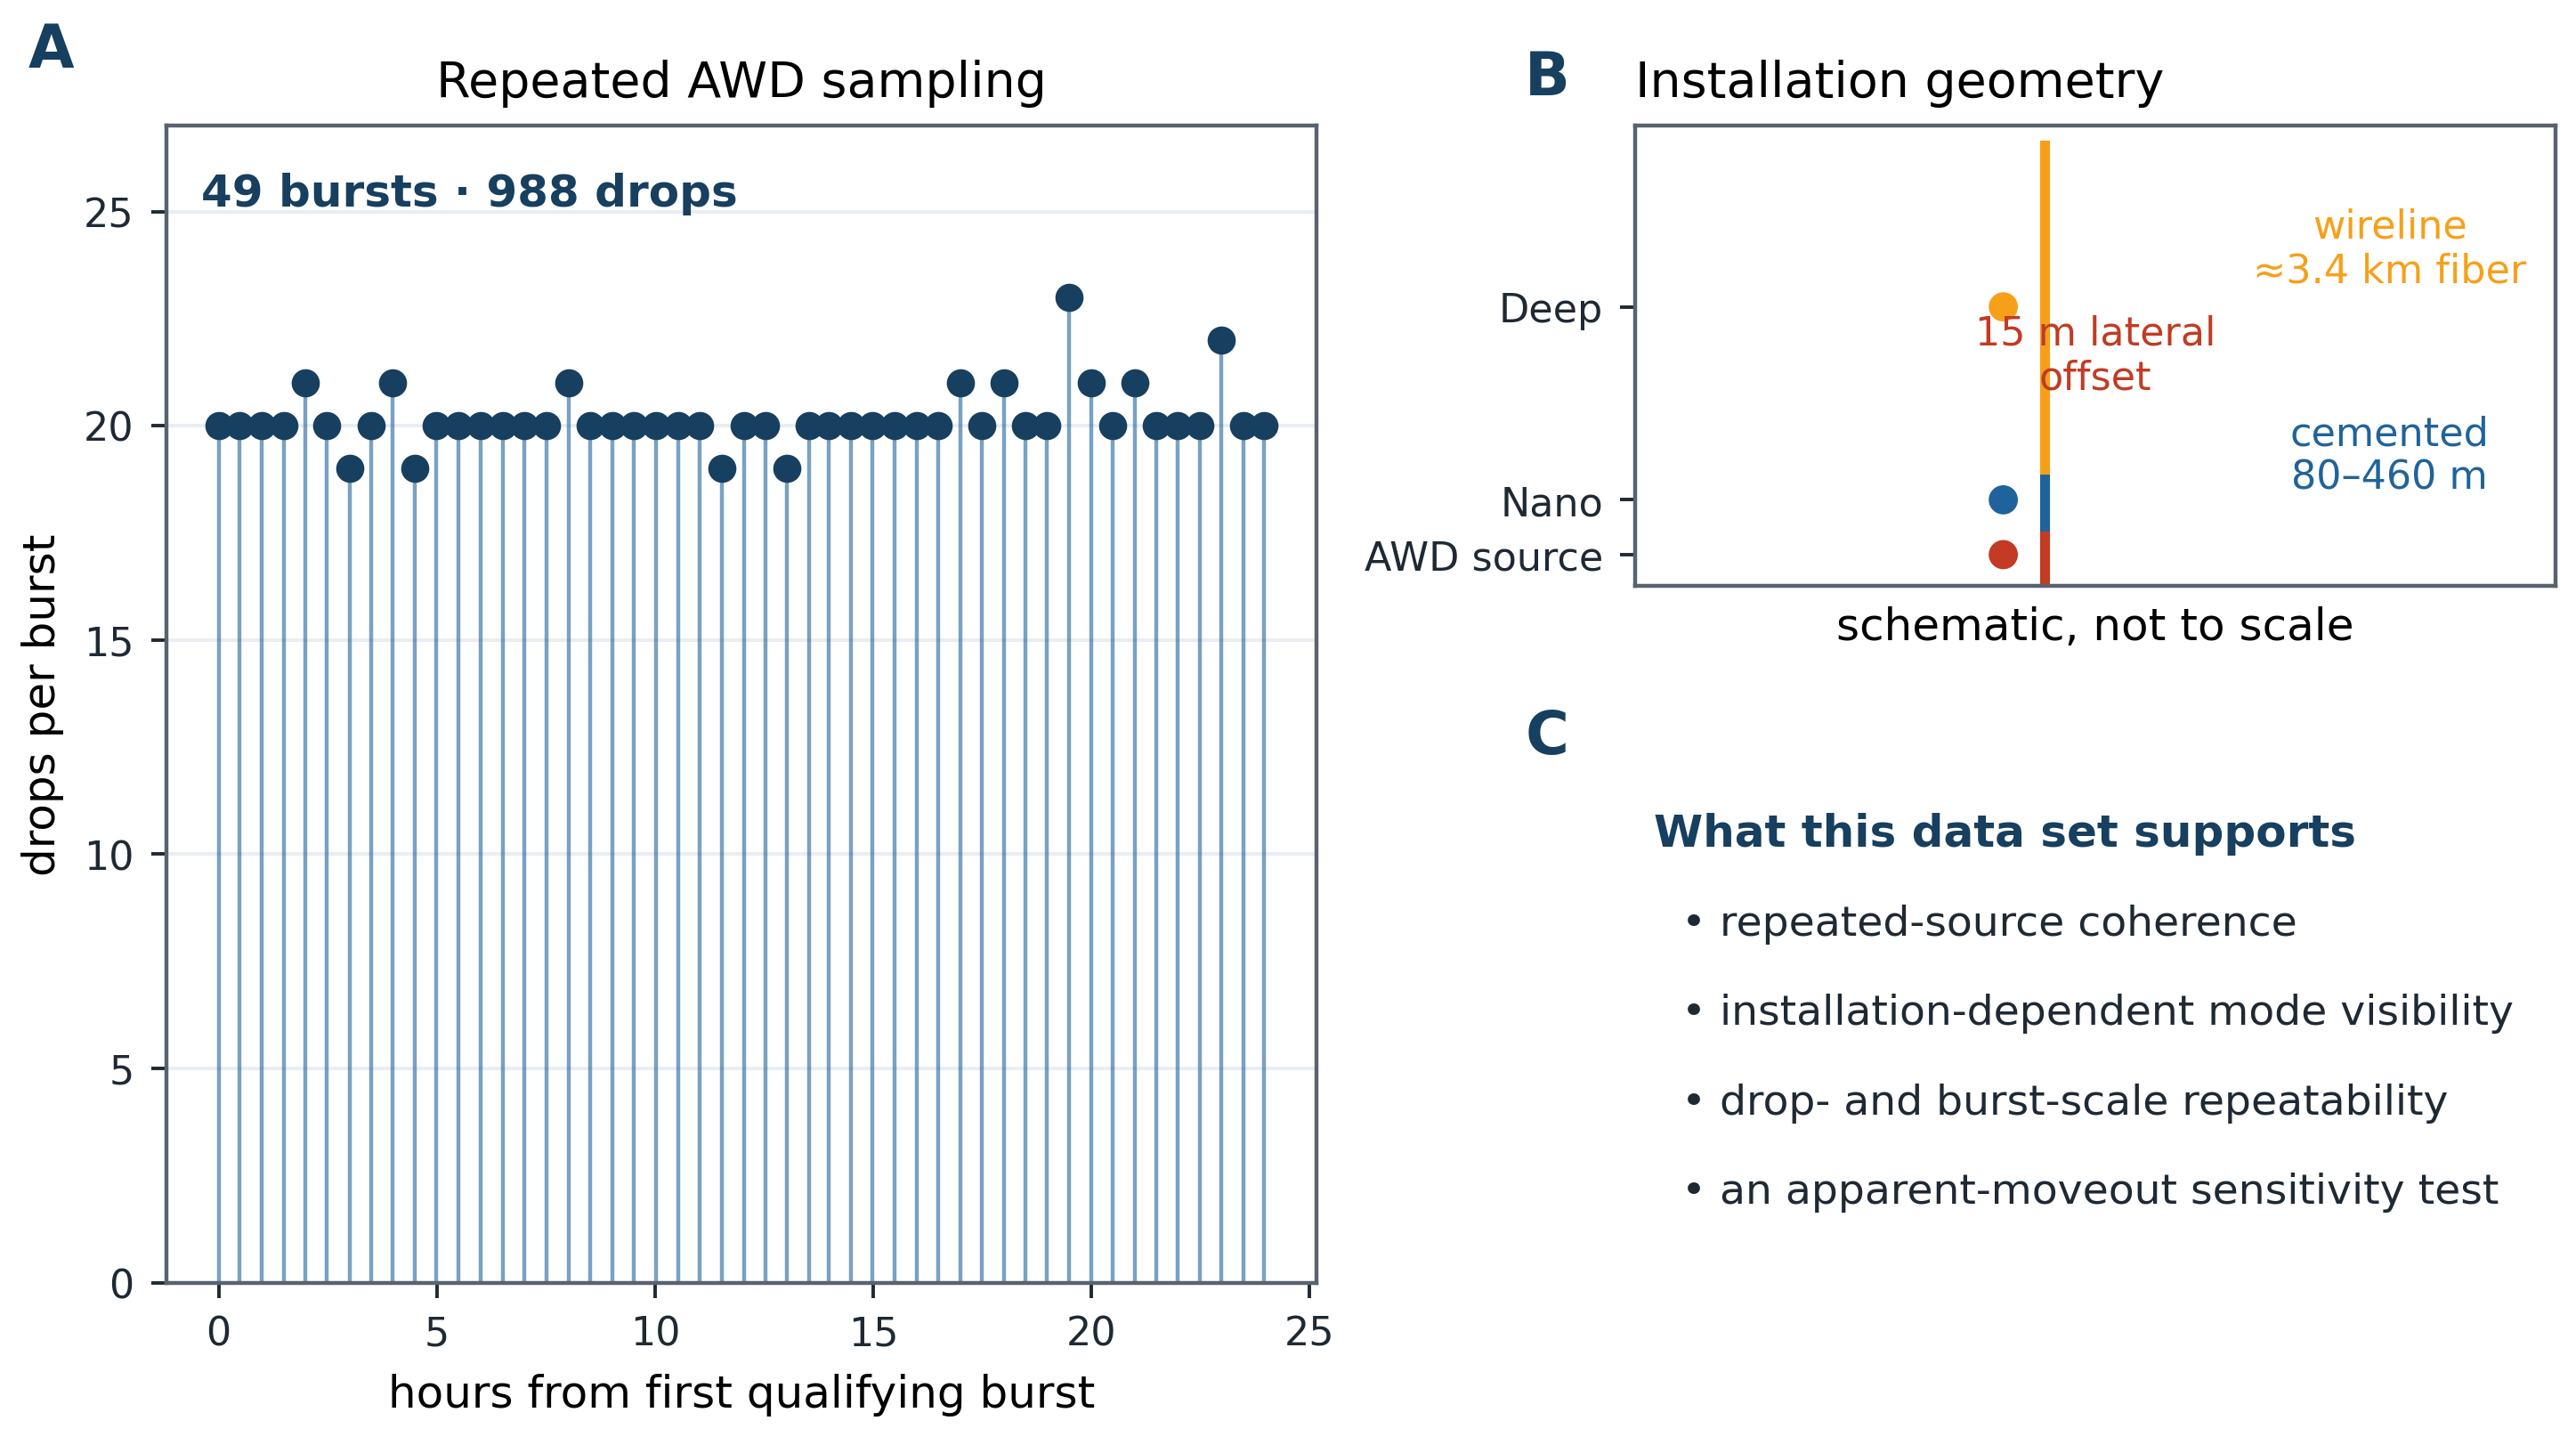
\includegraphics[width=0.88\linewidth]{../figures/awd_2026/core01_experiment_geometry.png}
\caption{\textbf{Core result 1: experiment and sampling geometry.} Burst timing and drop counts establish the repeated-source hierarchy: 49 qualifying bursts and 988 drops.  The right-hand schematic distinguishes the cemented Nano and wireline Deep installations and marks the approximate 15-m source offset.  It is an orientation diagram, not a surveyed depth map.}\end{figure}

\subsection{Core result 2: Nano mode and signed frequency--slowness}
\figquestion{Is the approximately 3-km-s$^{-1}$ Nano observation a spatially ordered mode with a stable propagation sign?}
\begin{figure}[H]
\centering
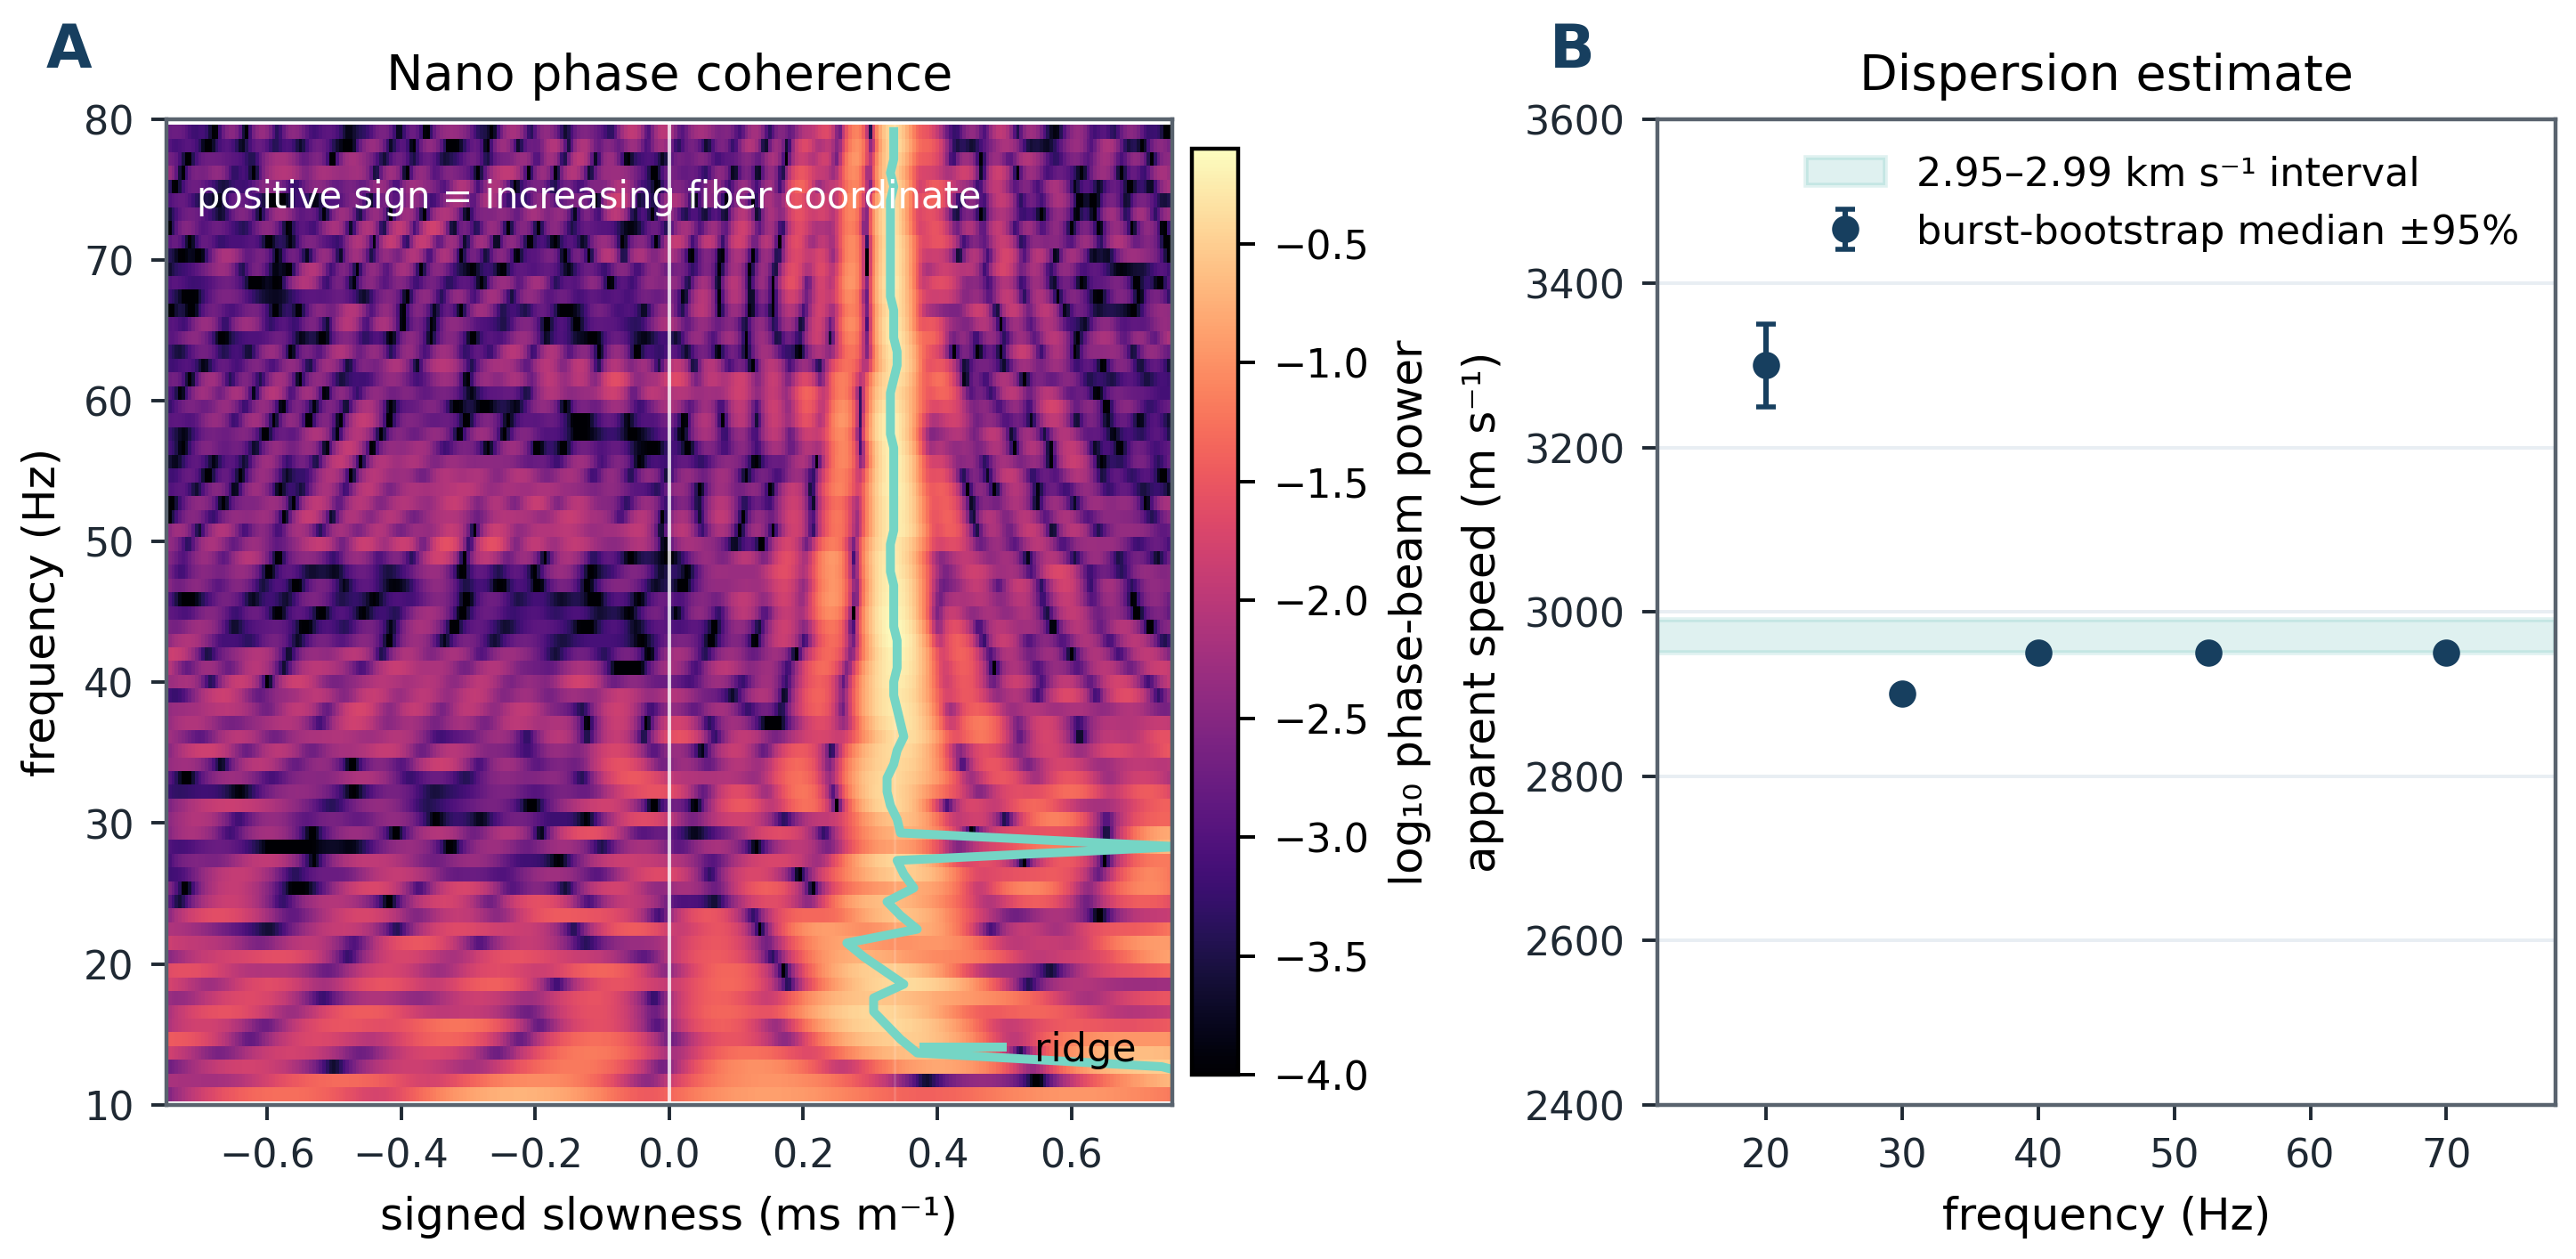
\includegraphics[width=0.88\linewidth]{../figures/awd_2026/core02_nano_mode_fk_dispersion.png}
\caption{\textbf{Core result 2: Nano signed frequency--slowness and dispersion.} Panel A shows the signed phase-beam spectrum for the 80--440-m Nano aperture; the positive-slowness ridge is the observed propagation direction.  Panel B shows frequency-binned apparent speeds and bootstrap intervals, with the 2.95--2.99-km-s$^{-1}$ interval shaded.  This establishes a coherent apparent mode and its frequency behavior, but does not by itself identify direct formation P.}\end{figure}

\subsection{Core result 3: Repeatability hierarchy}
\figquestion{Does the selected Nano moveout recur for individual drops, across bursts, and within independent substacks?}
\begin{figure}[H]
\centering
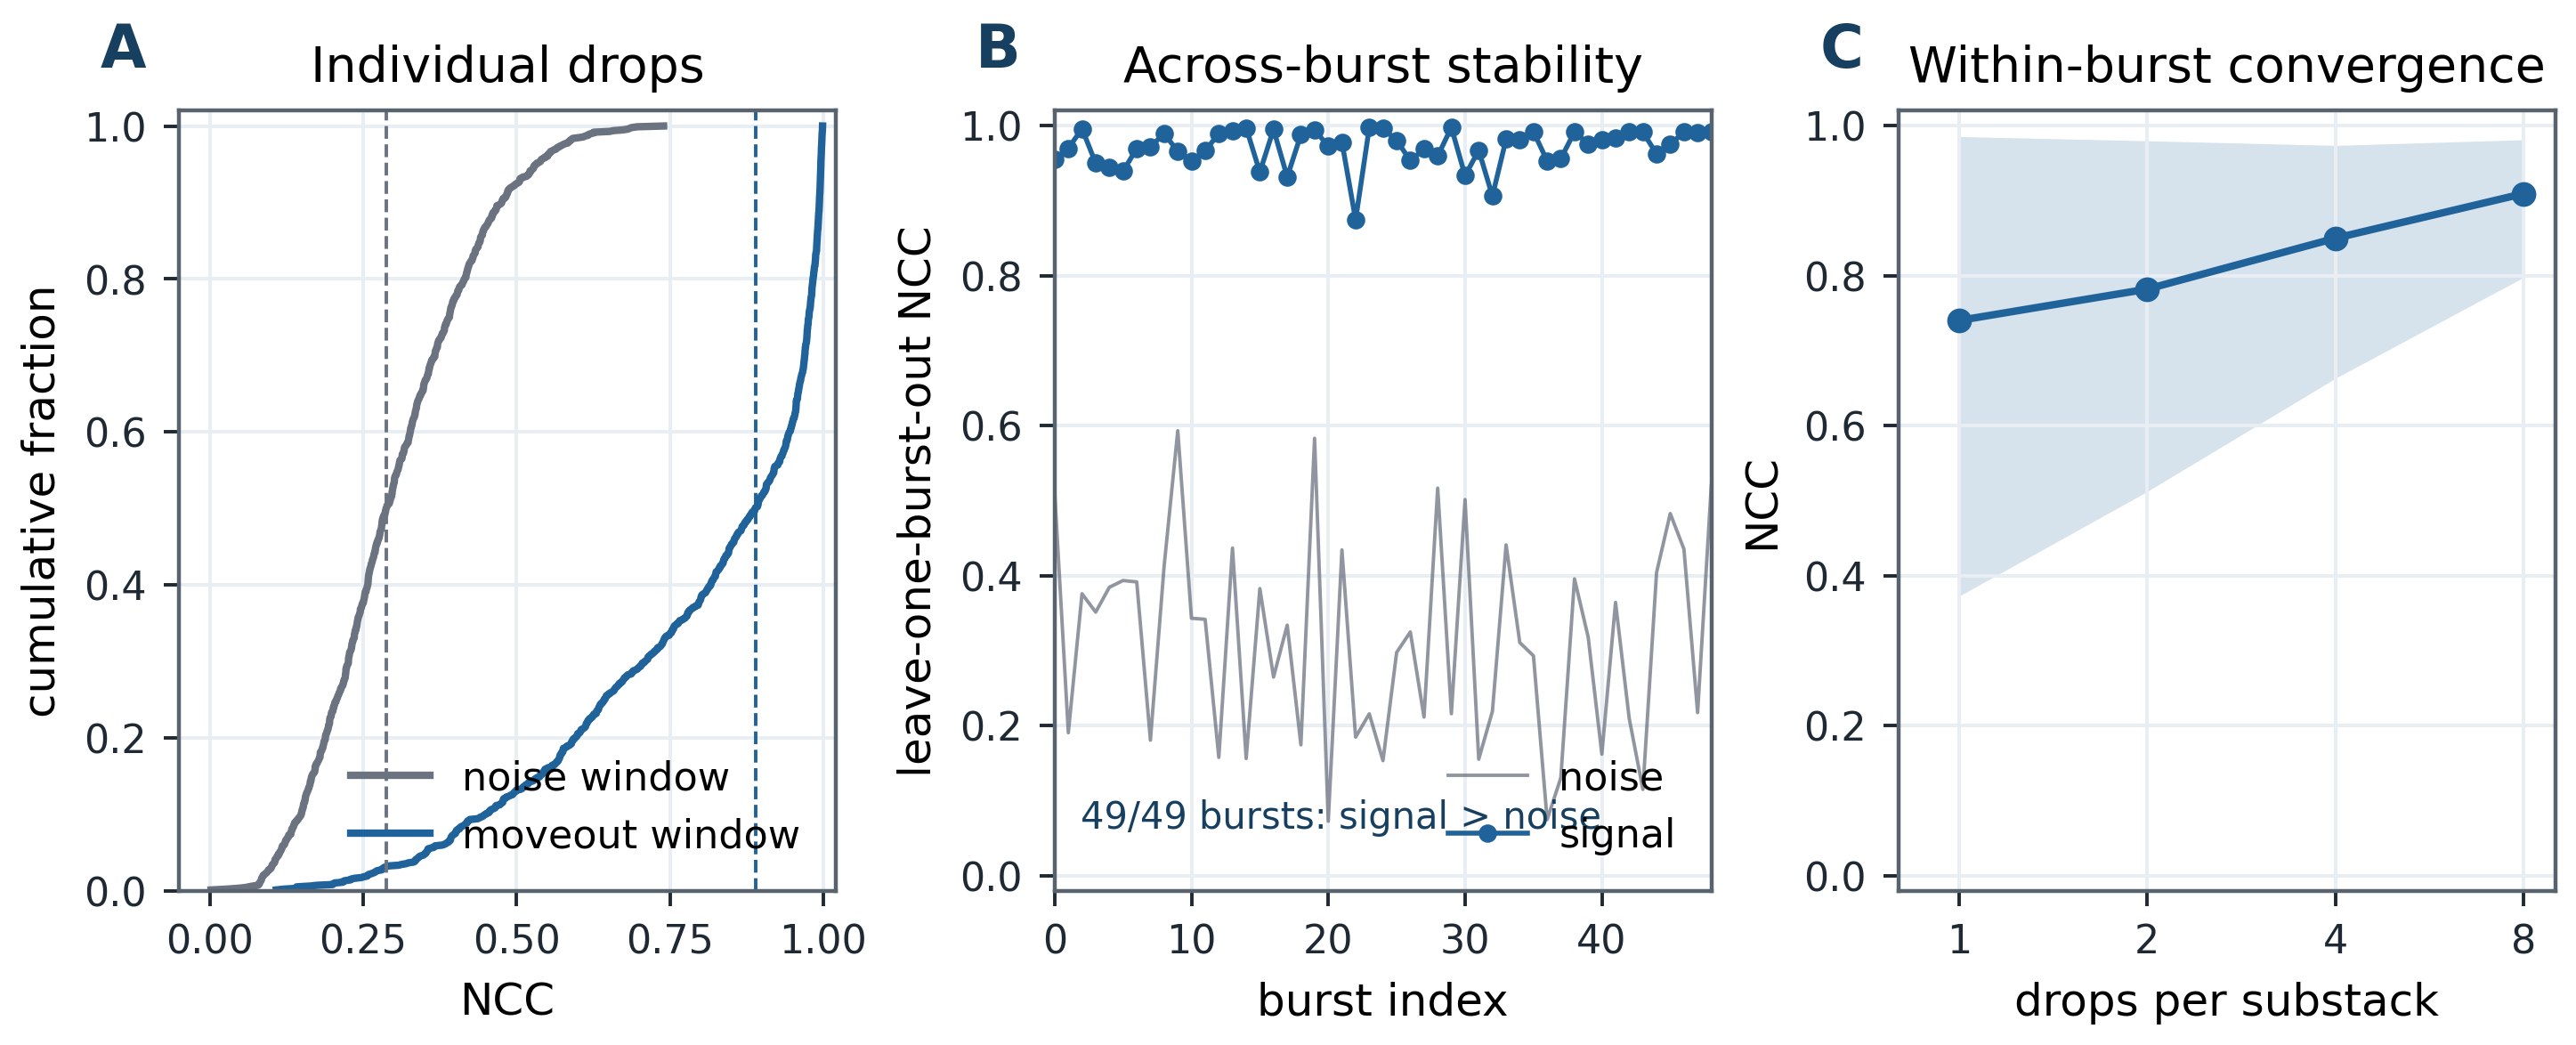
\includegraphics[width=0.88\linewidth]{../figures/awd_2026/core03_repeatability_hierarchy.png}
\caption{\textbf{Core result 3: repeatability at three source scales.} Panel A compares cumulative NCC distributions for 988 individual moveout windows and equal-duration noise windows.  Panel B shows leave-one-burst-out signal and noise NCC for all 49 bursts.  Panel C shows independent within-burst substack convergence.  The result supports source repeatability of the selected observable, not an amplitude-calibrated radiation or phase-identity claim.}\end{figure}

\subsection{Core result 4: Installation-dependent mode selection}
\figquestion{Do the cemented Nano and wireline Deep installations emphasize the same coherent mode?}
\begin{figure}[H]
\centering
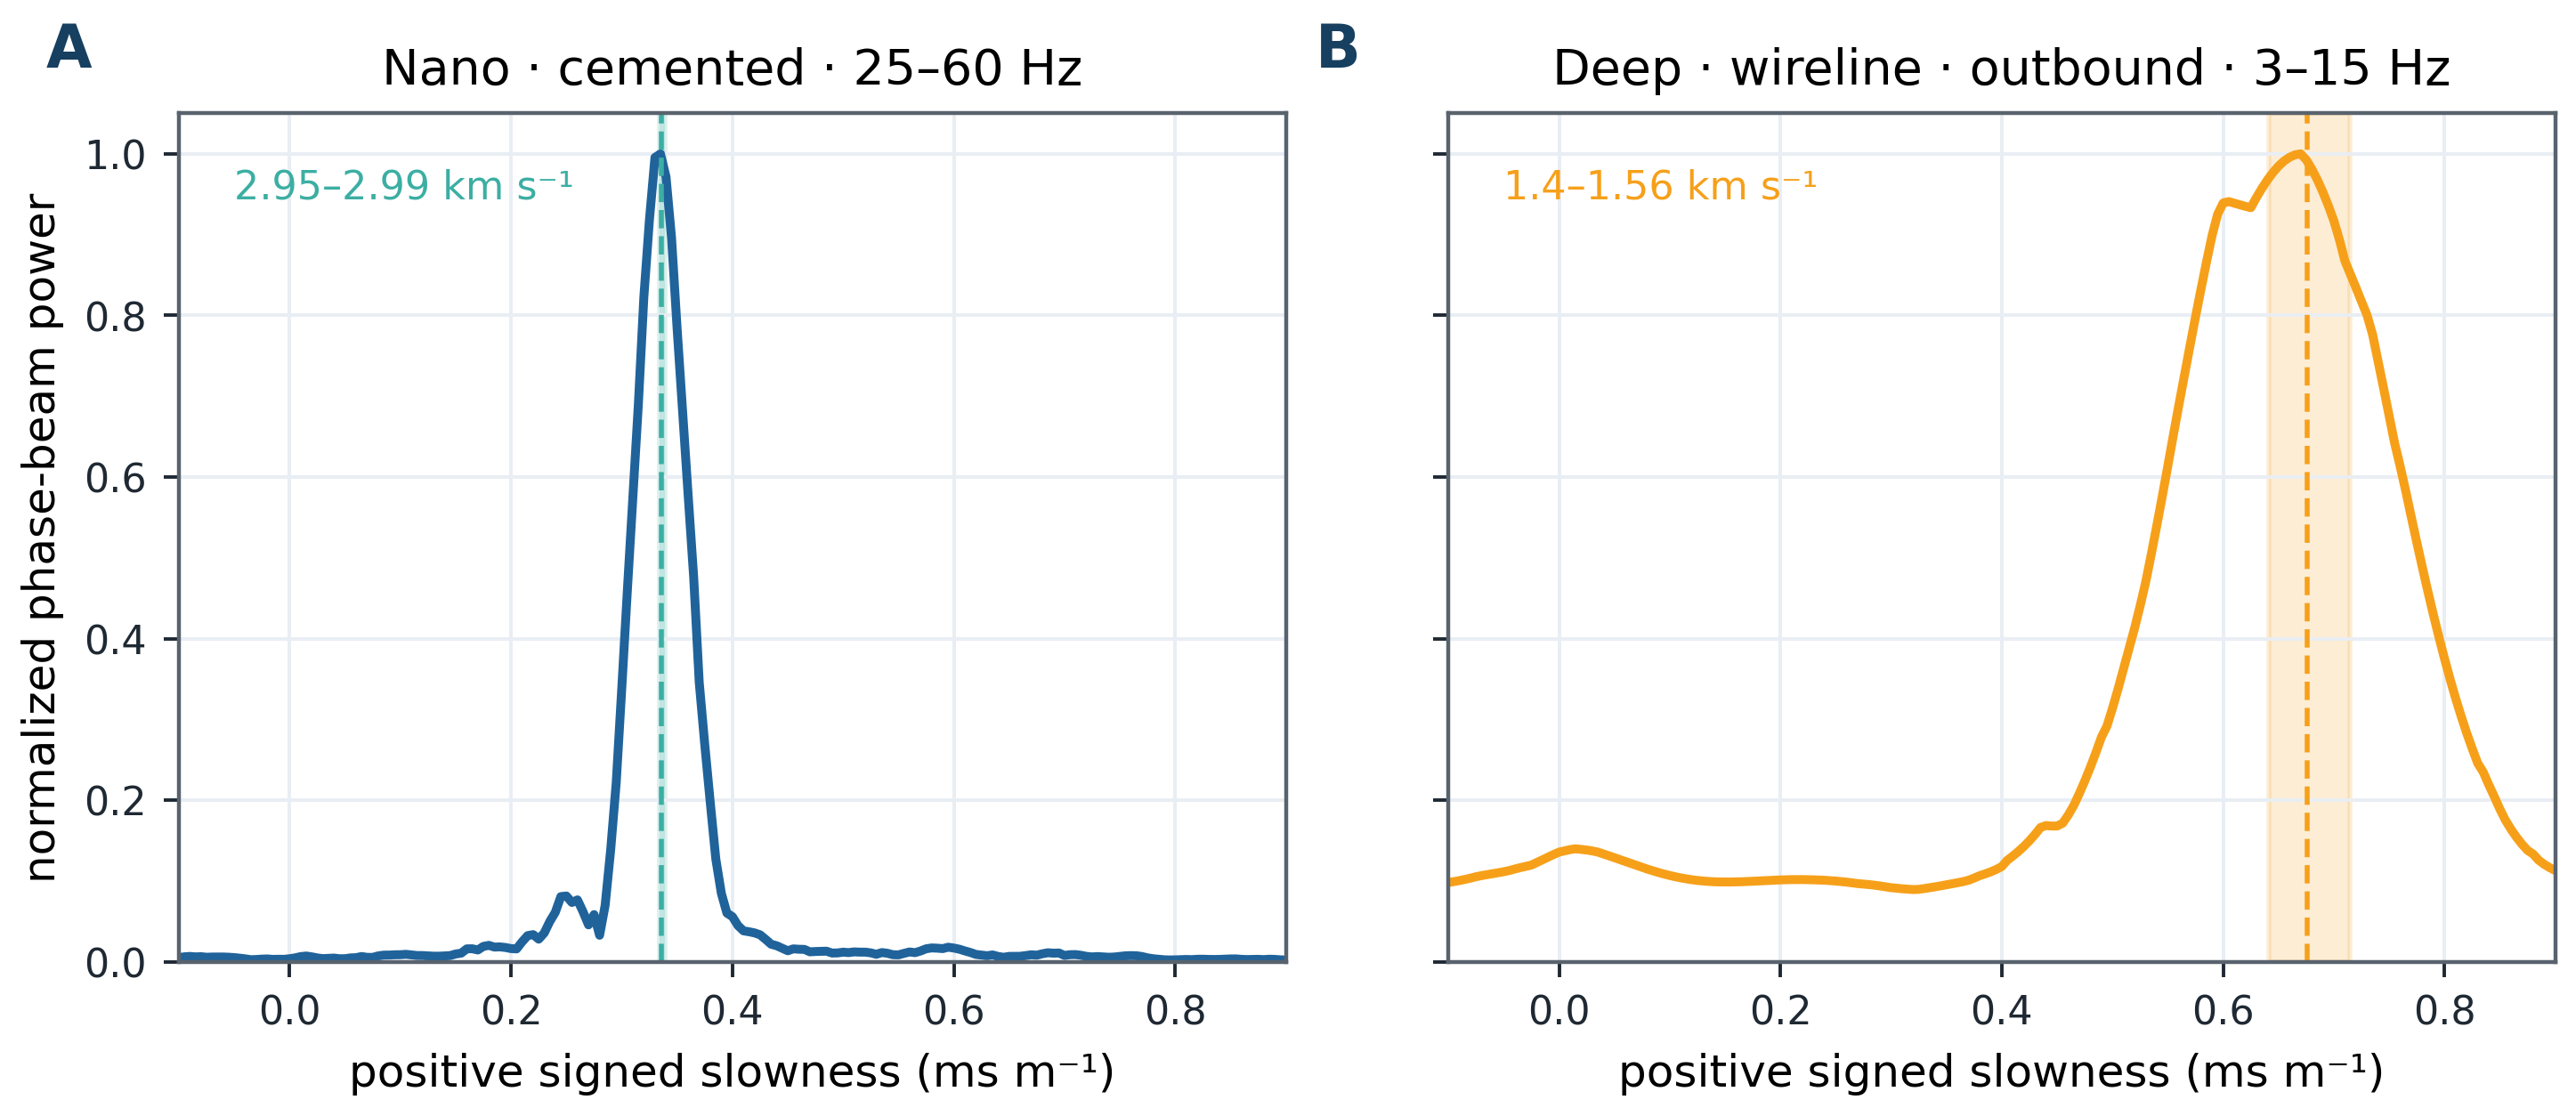
\includegraphics[width=0.88\linewidth]{../figures/awd_2026/core04_installation_mode_contrast.png}
\caption{\textbf{Core result 4: installation-dependent signed slowness.} The curves are normalized signed-slowness spectra from the accepted Nano 25--60-Hz aperture analysis and Deep outbound 3--15-Hz sliding-aperture analysis.  Shaded intervals mark the Nano 2.95--2.99-km-s$^{-1}$ and Deep 1.4--1.56-km-s$^{-1}$ apparent-speed ranges.  The comparison uses coherence and signed slowness, not uncalibrated absolute amplitude; the Deep feature remains a preliminary tube-wave interpretation.}\end{figure}

\subsection{Core result 5: Aperture and change sensitivity}
\figquestion{How far and at which frequencies is the Nano mode observable, and what apparent velocity change can the estimator recover?}
\begin{figure}[H]
\centering
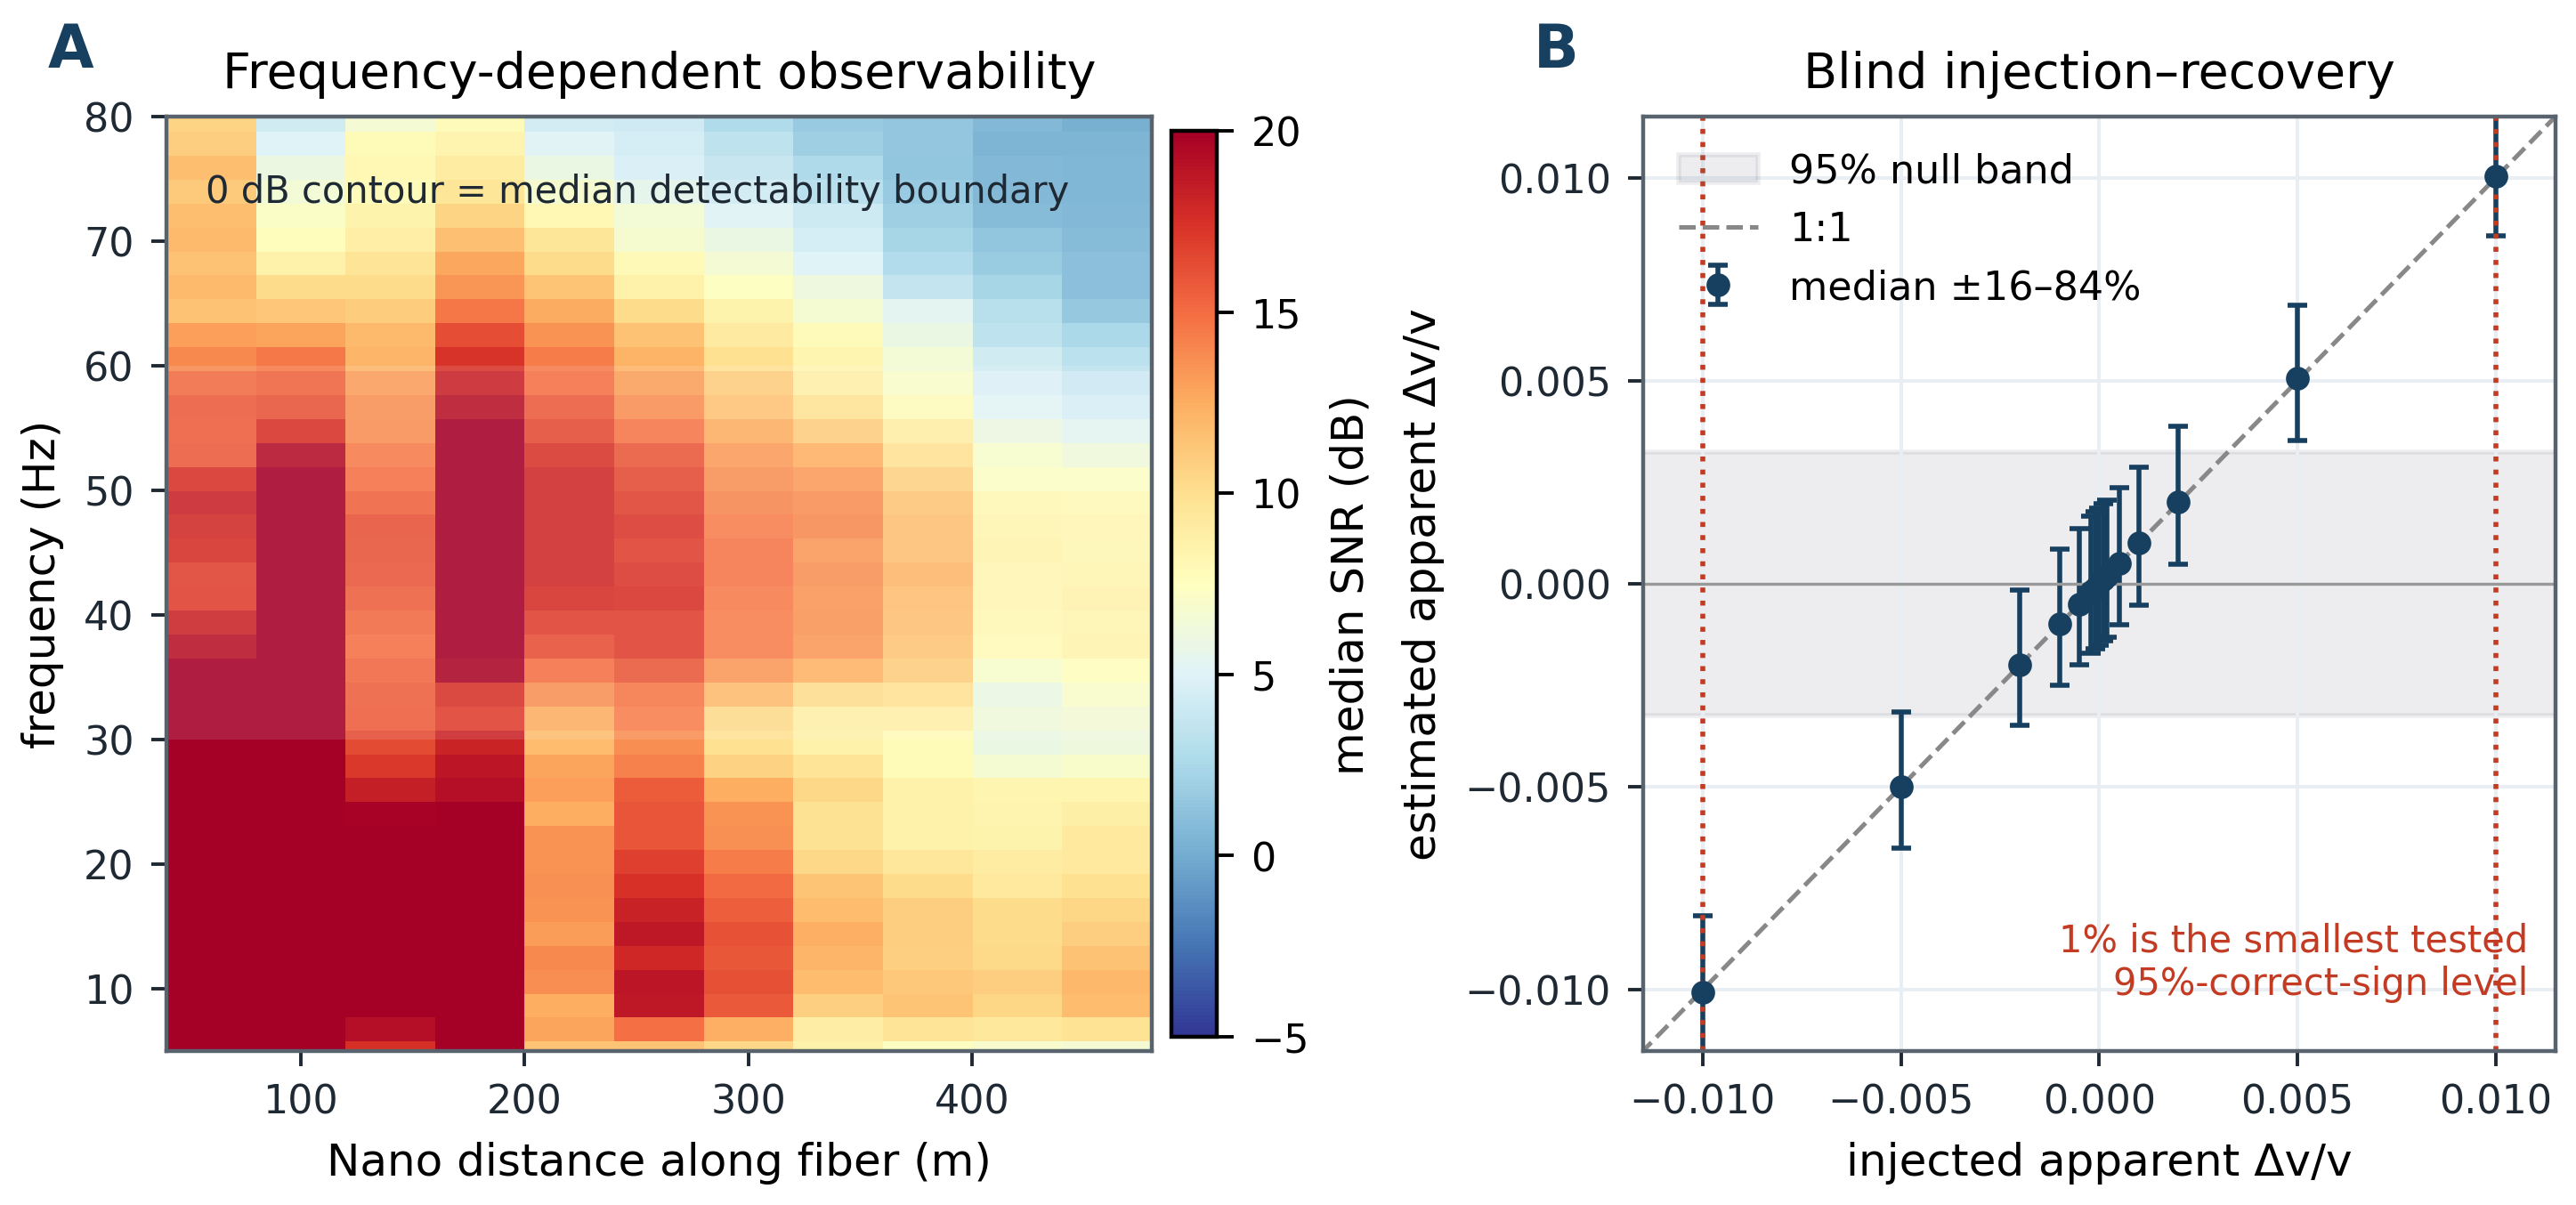
\includegraphics[width=0.88\linewidth]{../figures/awd_2026/core05_aperture_detection_limit.png}
\caption{\textbf{Core result 5: frequency-dependent aperture and injection--recovery.} Panel A shows median burst-level SNR versus distance and frequency; the dark contour marks 0 dB.  Panel B shows blind injection--recovery medians and central intervals against the 1:1 line, with the measured null band and $\pm1\%$ tested levels explicit.  The 1\% result is a limit for the selected apparent-moveout observable, not a demonstrated natural Parkfield $dv/v$ capability.}\end{figure}

\subsection{Core result 6: PGSI calibration and conditional registration}
\figquestion{Does the independent explosion data provide a timing and moveout constraint for the Nano interpretation?}
\begin{figure}[H]
\centering
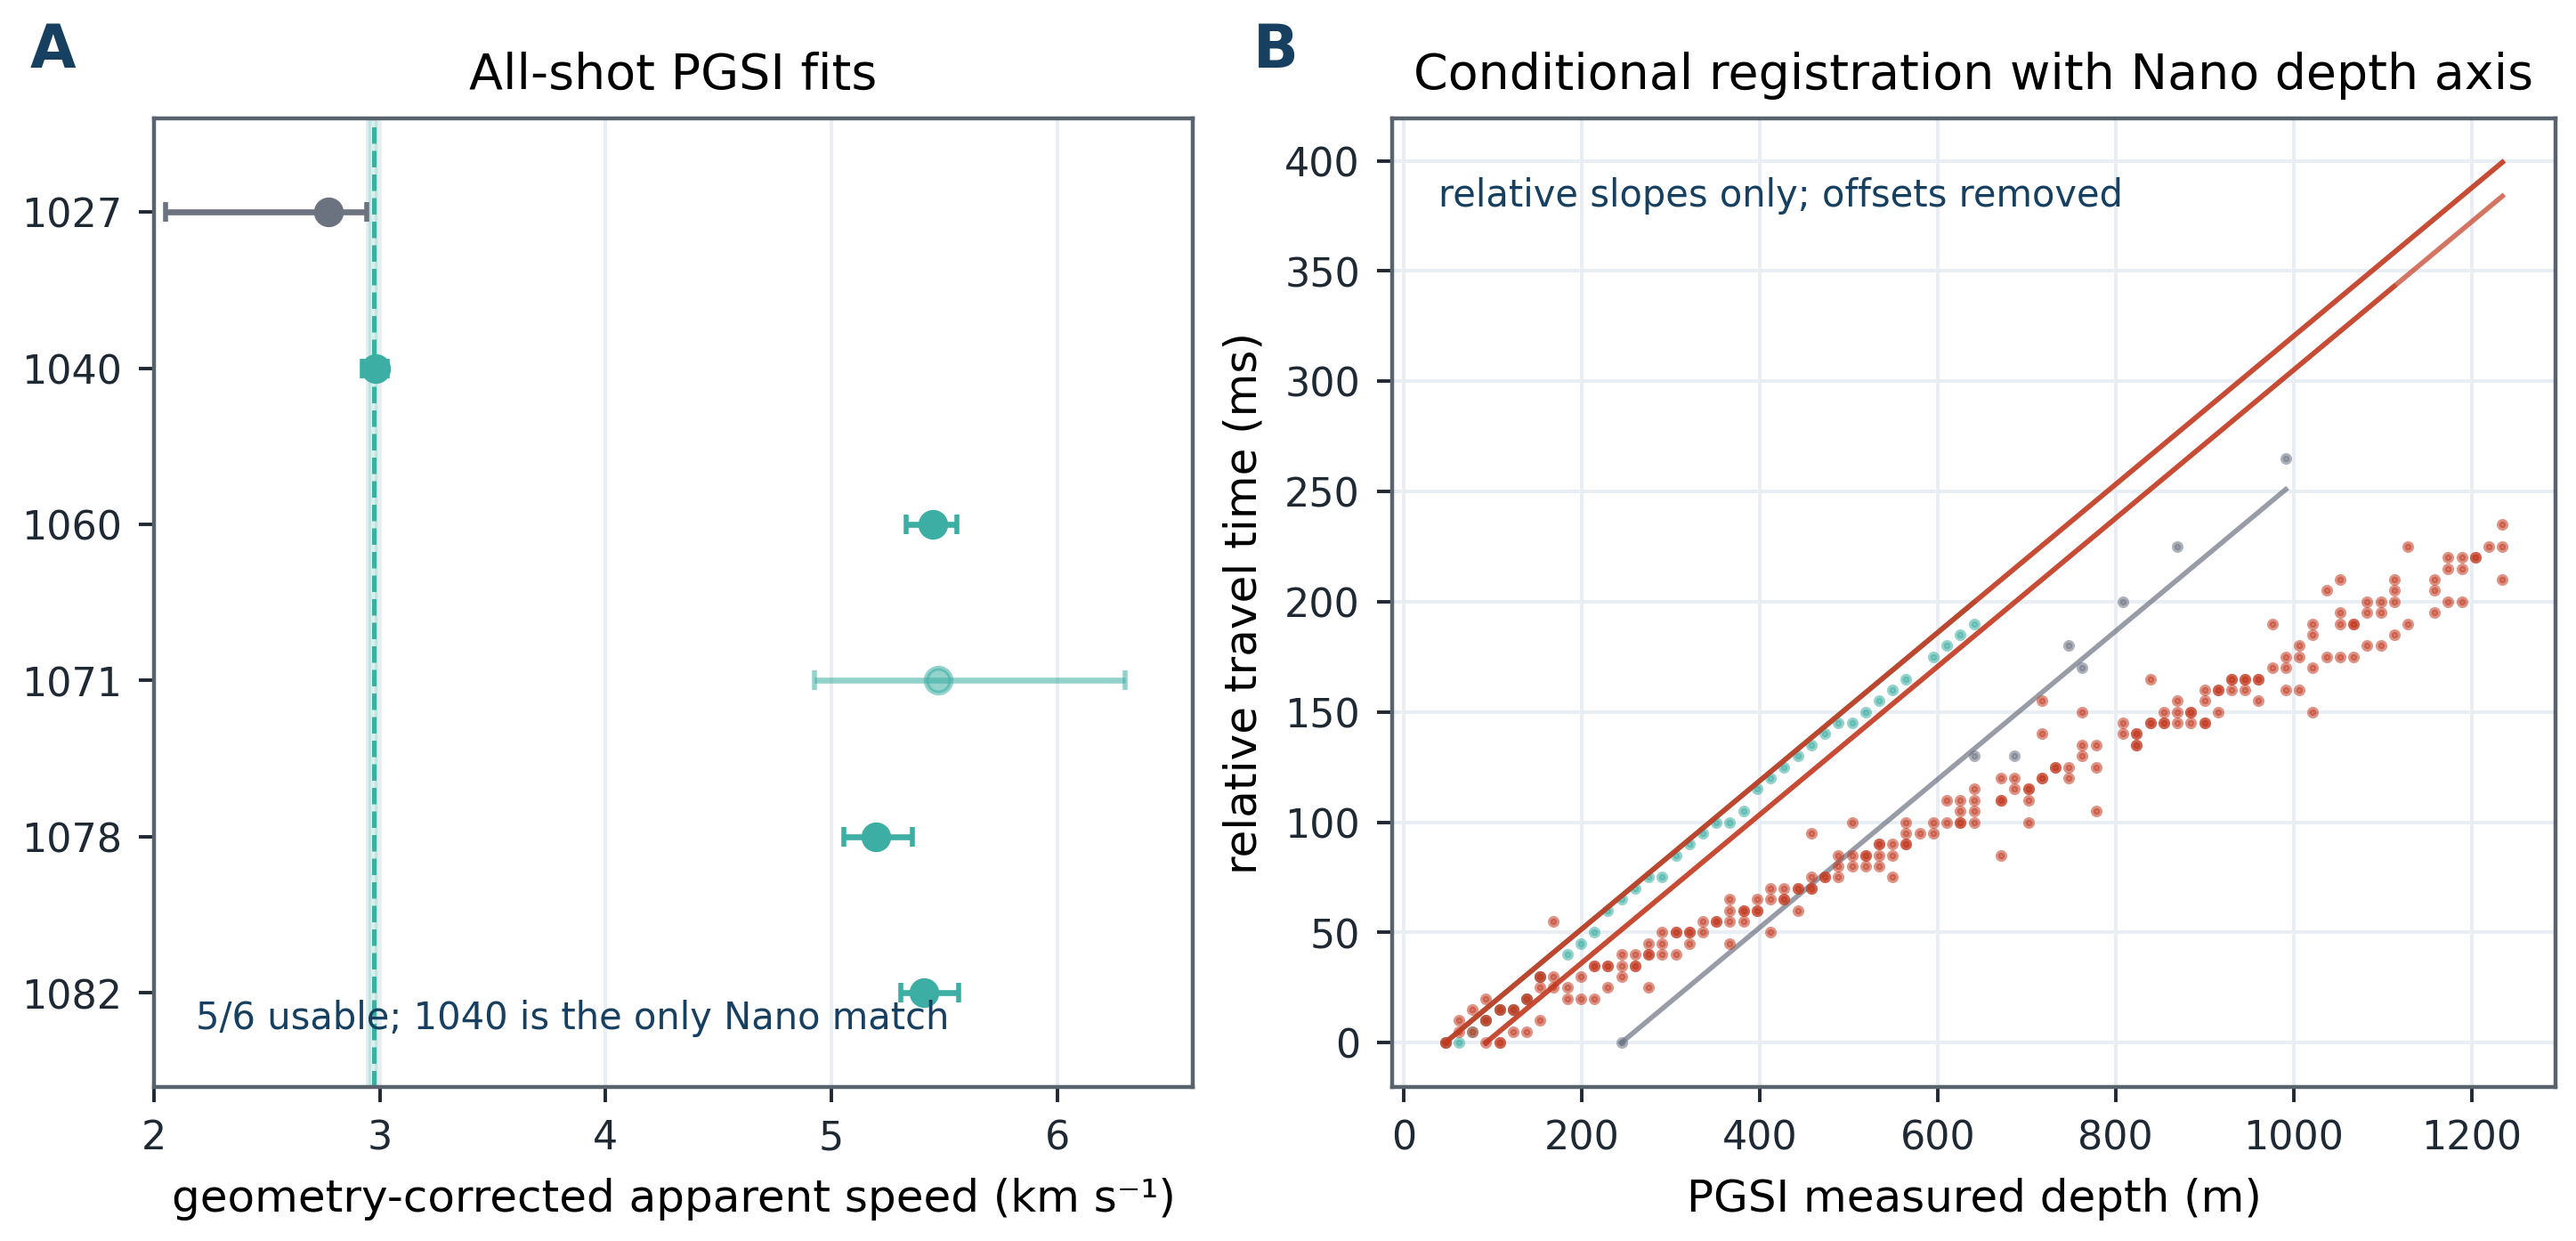
\includegraphics[width=0.88\linewidth]{../figures/awd_2026/core06_pgsi_calibration_registration.png}
\caption{\textbf{Core result 6: PGSI calibration and conditional Nano registration.} Panel A summarizes all six geometry-corrected fits under the common $t=i/200-0.200$-s convention; five pass fixed QC and shot 1040 is the only fit in the Nano interval.  Panel B compares relative PGSI travel-time slopes against measured depth with origin offsets removed.  This is a conditional registration and phase-identification constraint, not an absolute PGSI-to-Nano depth map or a $V_P$ inversion.}\end{figure}



The figure notes below distinguish established measurements, preliminary
interpretations, and planned follow-up tests.  Notebook flags, captions, and
conclusions should remain synchronized when the results are updated.

\subsection{Figure 1: What does the timing table mean?}
\figquestion{Can the timing-table value be treated as the AWD impact time, or
only as a repeatable alignment reference?}

The reference-node waveforms are stacked around code{UTC\_Date}; the shallow
Nano stack is shown on the same relative-time axis.  This is a timing audit, not
a velocity measurement.  In panel (a), the ensemble of node traces and their
weighted stack show where repeatable node energy lies relative to the timestamp.
Panel (b) shows the corresponding shallow Nano response.  Read the vertical
lines as empirical timing landmarks, not source-time corrections already
applied to the DAS.

\begin{figure}[H]
\centering
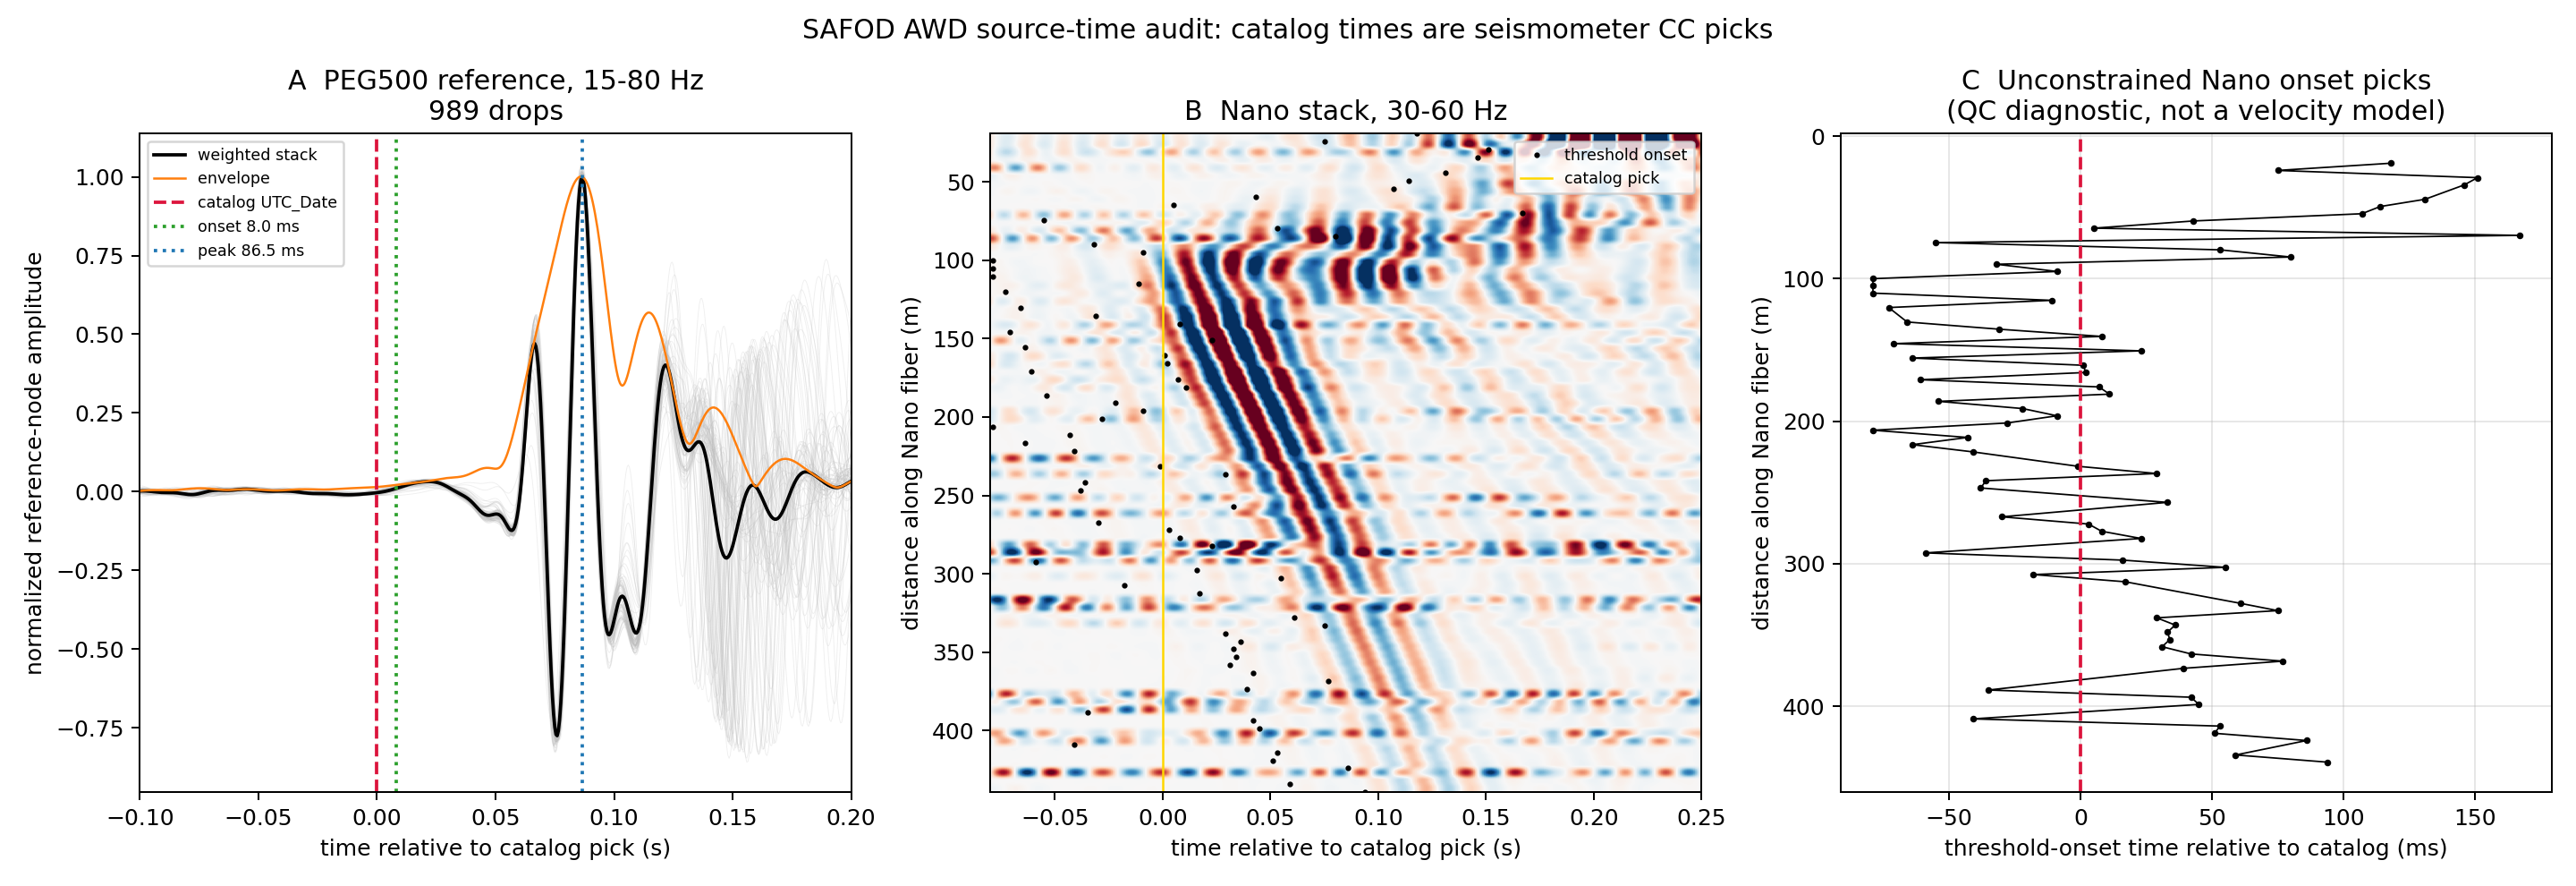
\includegraphics[width=\linewidth]{source_time_audit.png}
\caption{\textbf{Audit of the AWD alignment timestamp.} (a) Individual
15--80~Hz PEG500 vertical-component waveforms centered on the
\code{p26.cc9.txt UTC\_Date} values, with a squared-cross-correlation-weighted
stack and its envelope.  The red line is the table timestamp; the robust stack
envelope begins approximately 8.0~ms later and the largest absolute stacked
amplitude in the tested interval occurs approximately 86.5~ms later.  (b)
Shallow Nano DAS energy plotted relative to the same timestamps.  All 989
reference-node windows were recovered.  The experiment-wide consistency makes
\code{UTC\_Date} suitable for repeated-record alignment, but the observed
post-reference energy proves that it is not a physical impact trigger.  Absolute
DAS travel time therefore requires a separate source-time calibration; relative
moveout does not.}
\end{figure}

\takeaway{\accepted: use code{UTC\_Date} for alignment and state the reference
literally.  Do not call it an origin time, impact time, catalog pick, or DAS
arrival pick.}

\subsection{Figure 2: Is the Nano ridge visible before statistical scanning?}
\figquestion{Does the approximately $3~\mathrm{km\,s^{-1}}$ solution correspond
to a visible, ordered arrival, or only to a numerical maximum?}

The full same-drop Nano stack is plotted without independent trace
normalization.  A broad-band panel establishes context, the 30--60~Hz panel
shows the band where coherence is strongest, and the aligned panel shifts each
channel along the best trajectory.  A real trajectory should look sloped before
alignment and sharpen after alignment.

\begin{figure}[H]
\centering
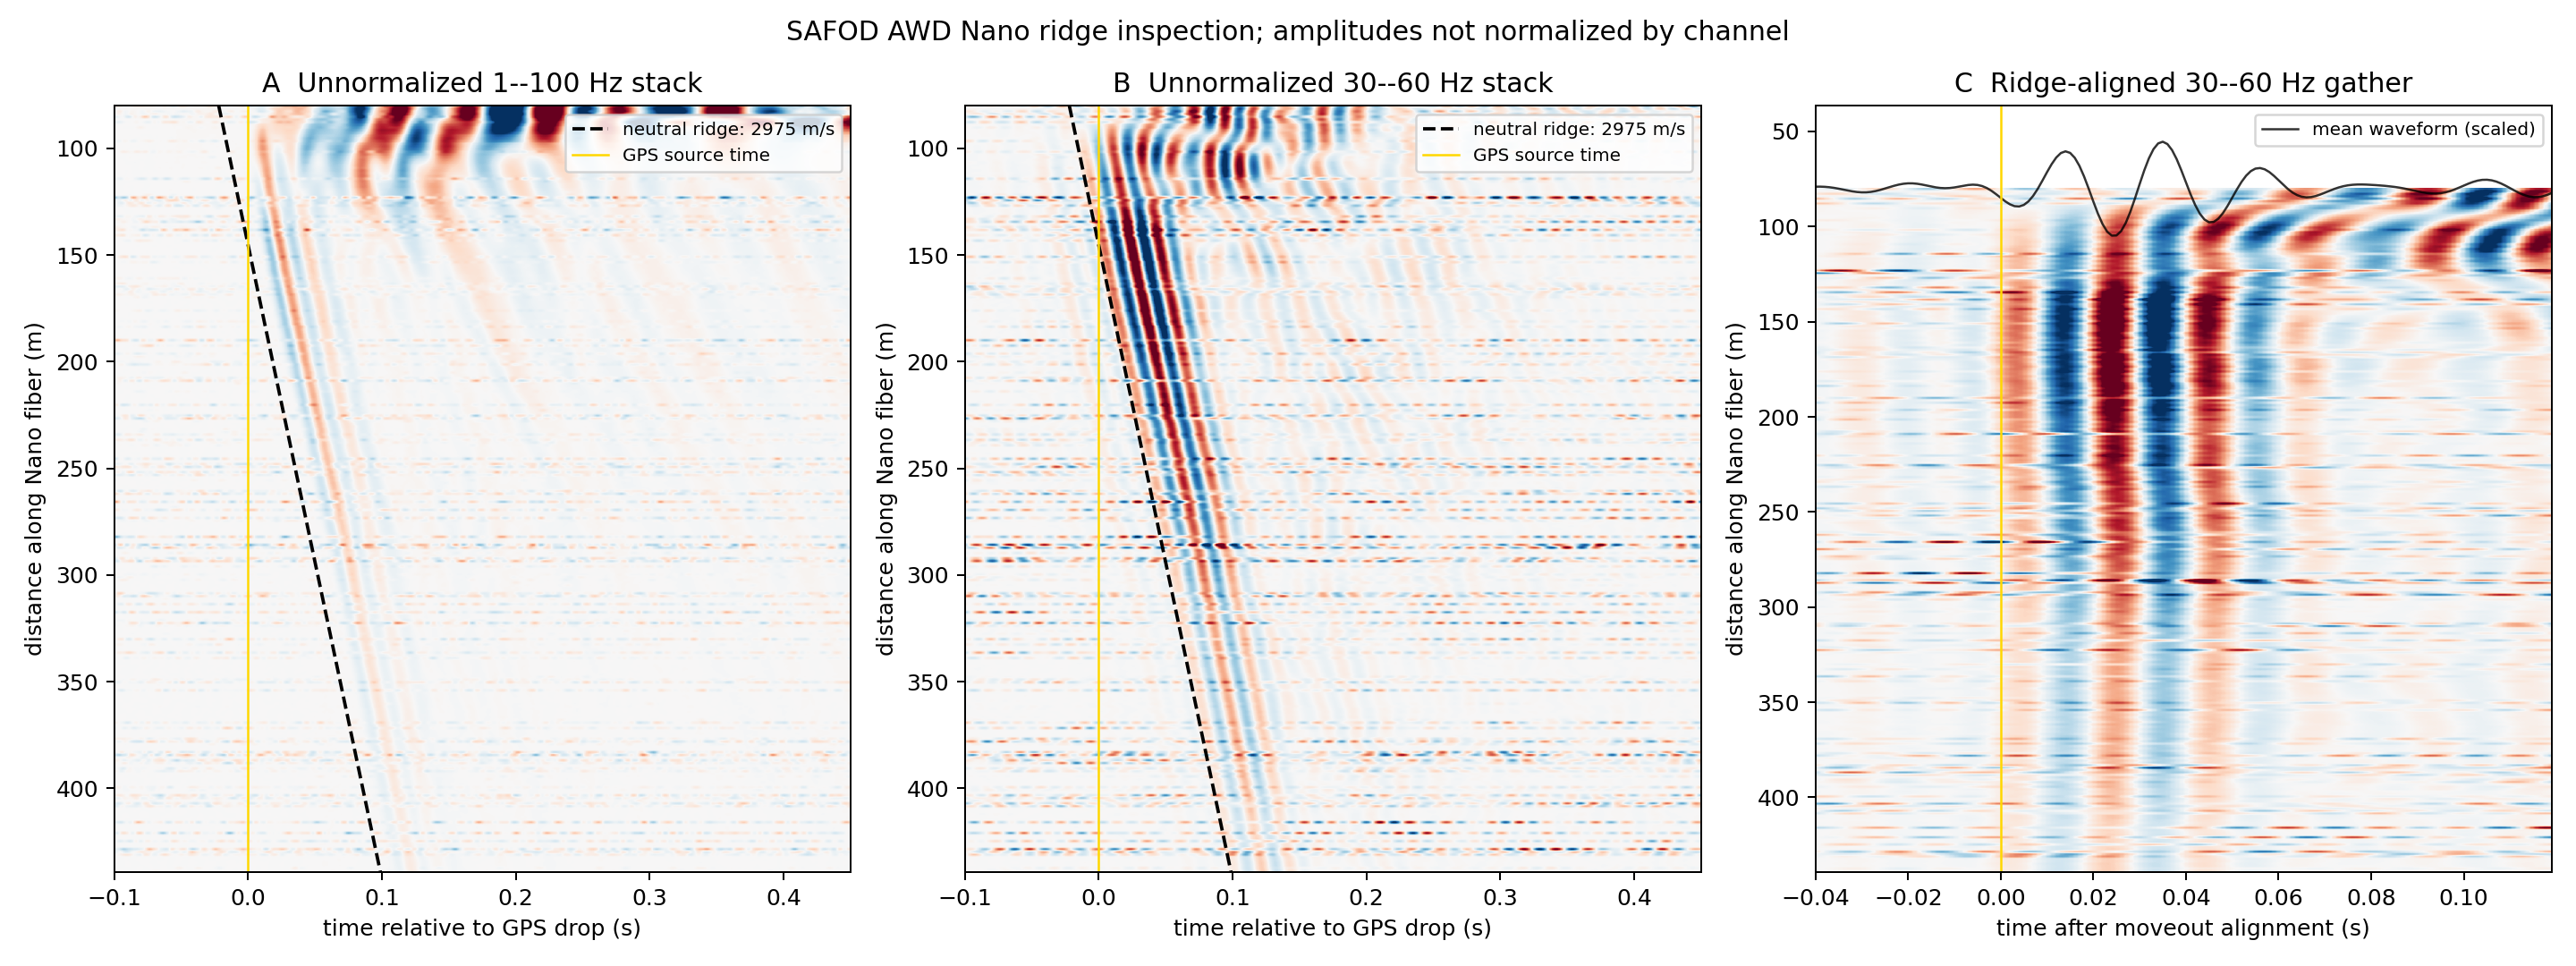
\includegraphics[width=\linewidth]{record_section_inspection.png}
\caption{\textbf{Visual and moveout-aligned inspection of the Nano coherent
mode.} The count-weighted stack contains the 859 complete same-drop observations
from 46 paired bursts and is restricted to 80--440~m along Nano fiber.  The
record sections retain a common amplitude definition rather than normalizing
every channel independently.  The black dashed trajectory is the phase-neutral
local-semblance optimum, approximately $2.975~\mathrm{km\,s^{-1}}$ with a
$-22$~ms intercept relative to code{p26.cc9.txt UTC\_Date}.  The 30--60~Hz ridge
has systematic positive moveout with increasing fiber coordinate and becomes
more compact when channels are shifted along the predicted trajectory.  This
figure demonstrates a visually ordered wavefield feature; it does not establish
that the feature is direct P.}
\end{figure}

\takeaway{\accepted: the Nano feature is visibly present and spatially ordered;
it is not merely a plotting or optimization artifact.}

\subsection{Figure 3: Which apparent speeds carry coherent energy?}
\figquestion{What constant-velocity trajectories maximize coherence on matched
Nano and Deep apertures, and how do those maxima change with frequency?}

Each color map is a search over trial speed and relative-time intercept.  Peaks
are candidates, not phase labels.  The matched 80--440~m interval makes the
initial Nano--Deep comparison spatially consistent, but it does not make the
installations or physical depths equivalent.

\begin{figure}[H]
\centering
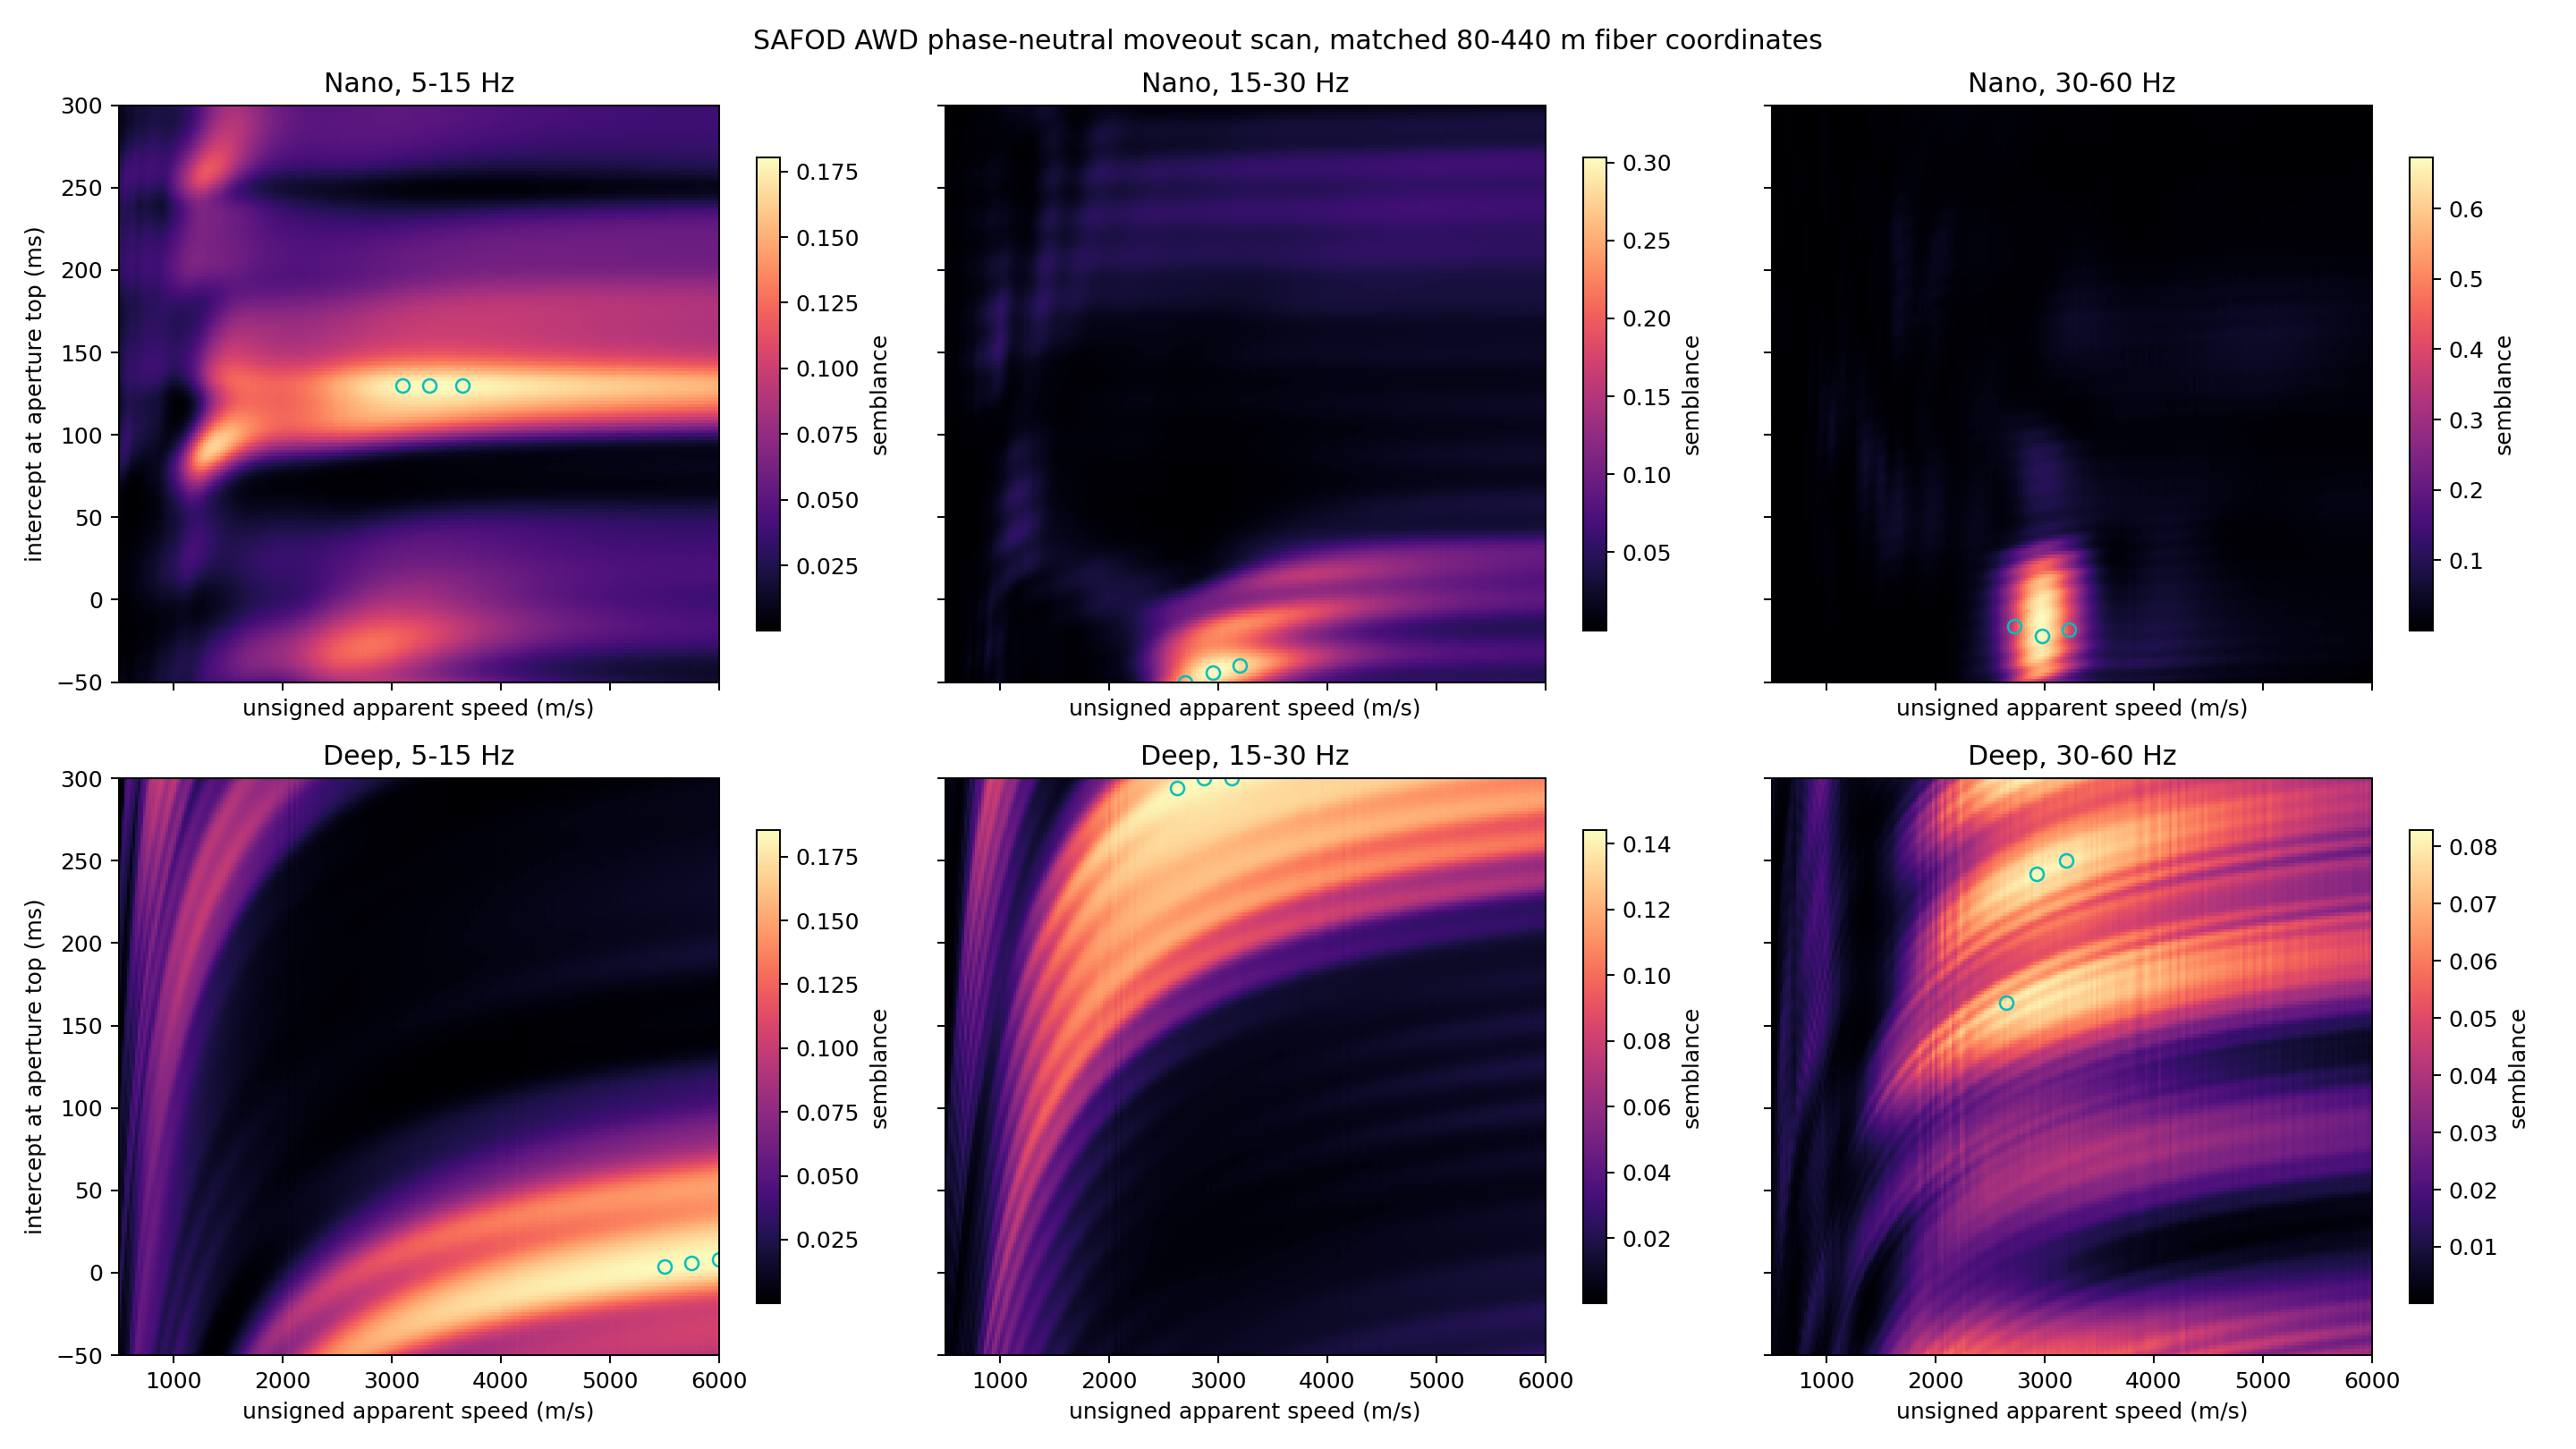
\includegraphics[width=\linewidth]{mode_scan.png}
\caption{\textbf{Phase-neutral constant-velocity moveout scans.} Rows compare
cemented Nano and wireline Deep data over the same 80--440~m along-fiber
aperture; columns show 5--15, 15--30, and 30--60~Hz bands.  For each trial speed
from 500 to $6{,}000~\mathrm{m\,s^{-1}}$ and trial intercept from $-50$ to
$+300$~ms, waveform coherence is evaluated along a linear moveout trajectory.
Color denotes semblance, and marked local maxima identify separated candidate
speeds rather than preassigned P, S, or tube-wave phases.  Nano contains a
dominant 30--60~Hz maximum near $2.975~\mathrm{km\,s^{-1}}$ and a weaker
15--30~Hz counterpart.  The same shallow Deep interval has substantially lower
coherence, showing that identical source events do not produce the same
dominant shallow wavefield on the two installations.}
\end{figure}

\takeaway{Nano has a robust near-$3~\mathrm{km\,s^{-1}}$ candidate.  The
full/matched Deep result is inconclusive and should not be interpreted as an
absence of Deep signal; localized, lower-frequency analysis is needed.}

\subsection{Figure 4: Could the Nano maximum happen by chance?}
\figquestion{Would comparable coherence appear if the observed channel ordering
were accidental, or if the same search were applied before the source-related
wavefield?}

The spatial null permutes channel order and repeats the local search, thereby
including the advantage of choosing the best speed and intercept.  The
pre-reference control asks whether coherent common-mode noise produces a similar
trajectory at earlier time.

\begin{figure}[H]
\centering
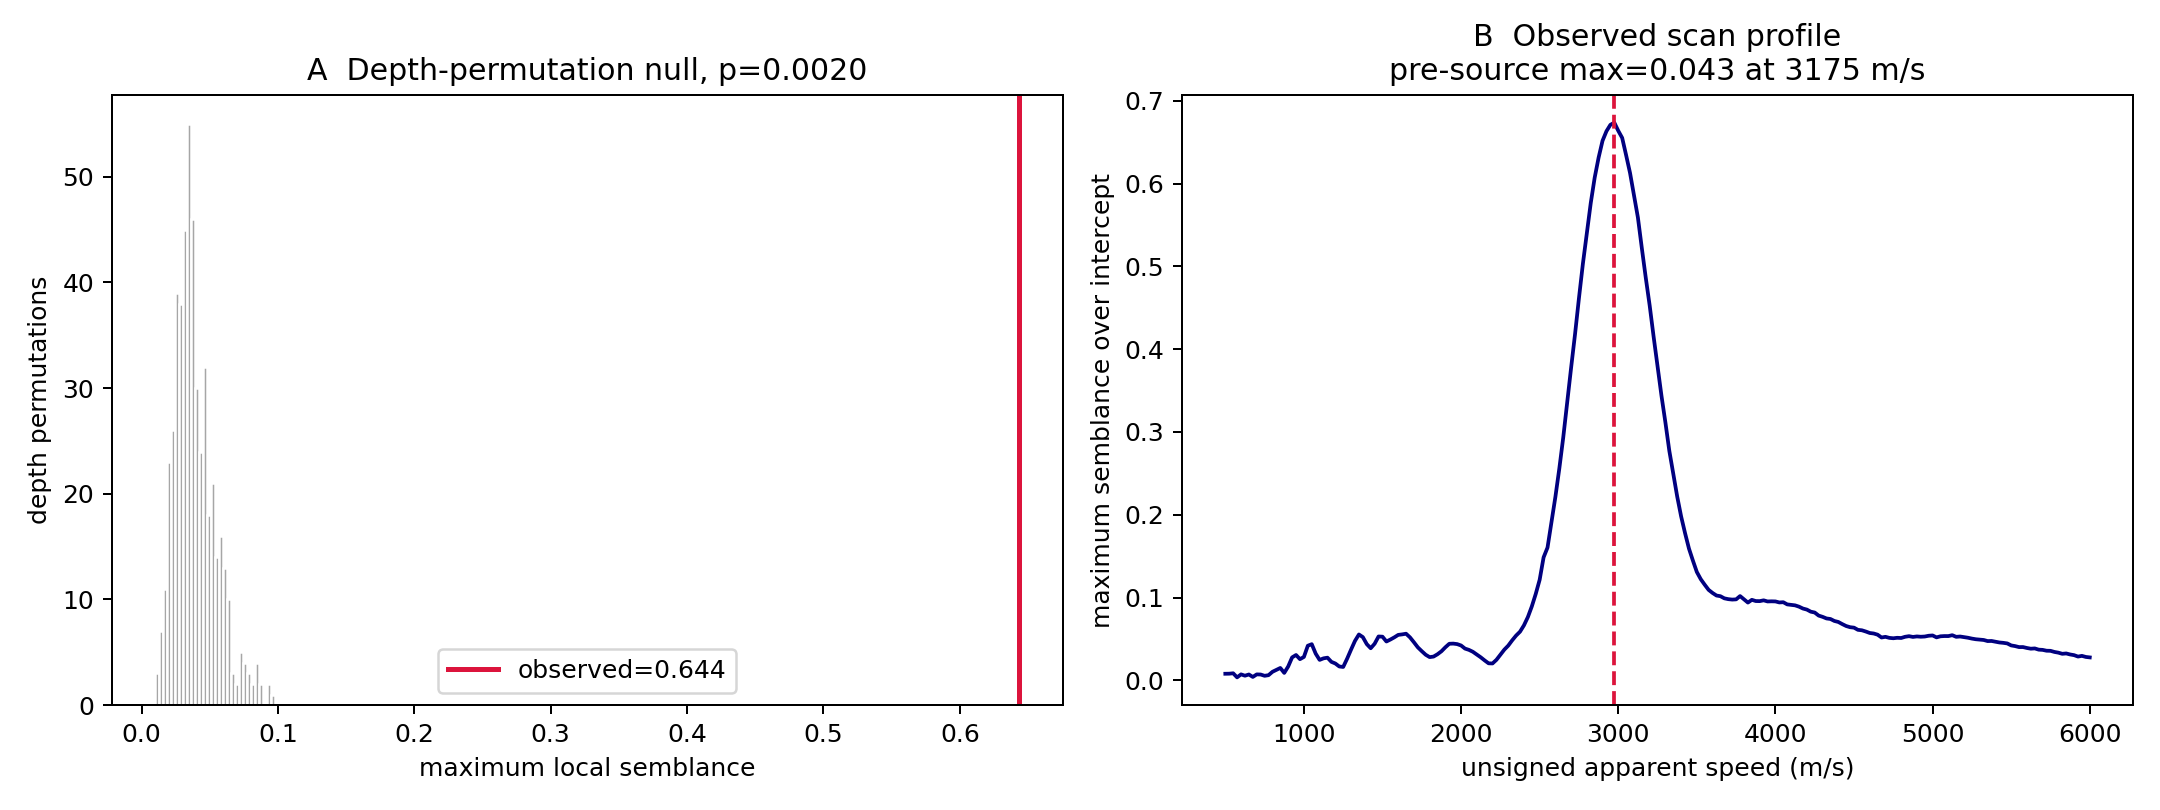
\includegraphics[width=0.94\linewidth]{null_tests.png}
\caption{\textbf{Phase-neutral null tests for the Nano 30--60~Hz moveout
maximum.} The gray distribution contains the largest local semblance from each
of 499 random channel-order permutations over the 80--440~m aperture.  Every
permutation preserves the temporal waveform at every channel and receives the
same local speed/intercept search as the observation.  The observed maximum is
0.644 at approximately $2.975~\mathrm{km\,s^{-1}}$ and $-22$~ms; it exceeds all
permuted maxima, giving the finite-sample, look-elsewhere-corrected value
$p=0.002$.  An independent pre-reference search finds a largest control
semblance of only 0.043.  These tests reject accidental spatial ordering and a
comparable pre-reference ridge under the tested nulls; they do not discriminate
direct P from guided energy.}
\end{figure}

\takeaway{\accepted: the coherent Nano mode is statistically significant under
the spatial-order test and is not reproduced by the pre-reference control.}

\subsection{Figure 5: Which way does the energy propagate?}
\figquestion{What is the sign of propagation, what is the corresponding apparent
slowness, and is a full-aperture $f$--$k$ description meaningful on each fiber?}

The horizontal axis is signed slowness.  Positive and negative values indicate
opposite directions along the displayed fiber coordinate.  A vertical ridge
would be nearly nondispersive; a ridge that bends systematically with frequency
is dispersive.  Blank or weak Deep full-leg panels are valid outcomes after
finite-channel QC, not legacy placeholders or dead-channel failures.

\begin{figure}[H]
\centering
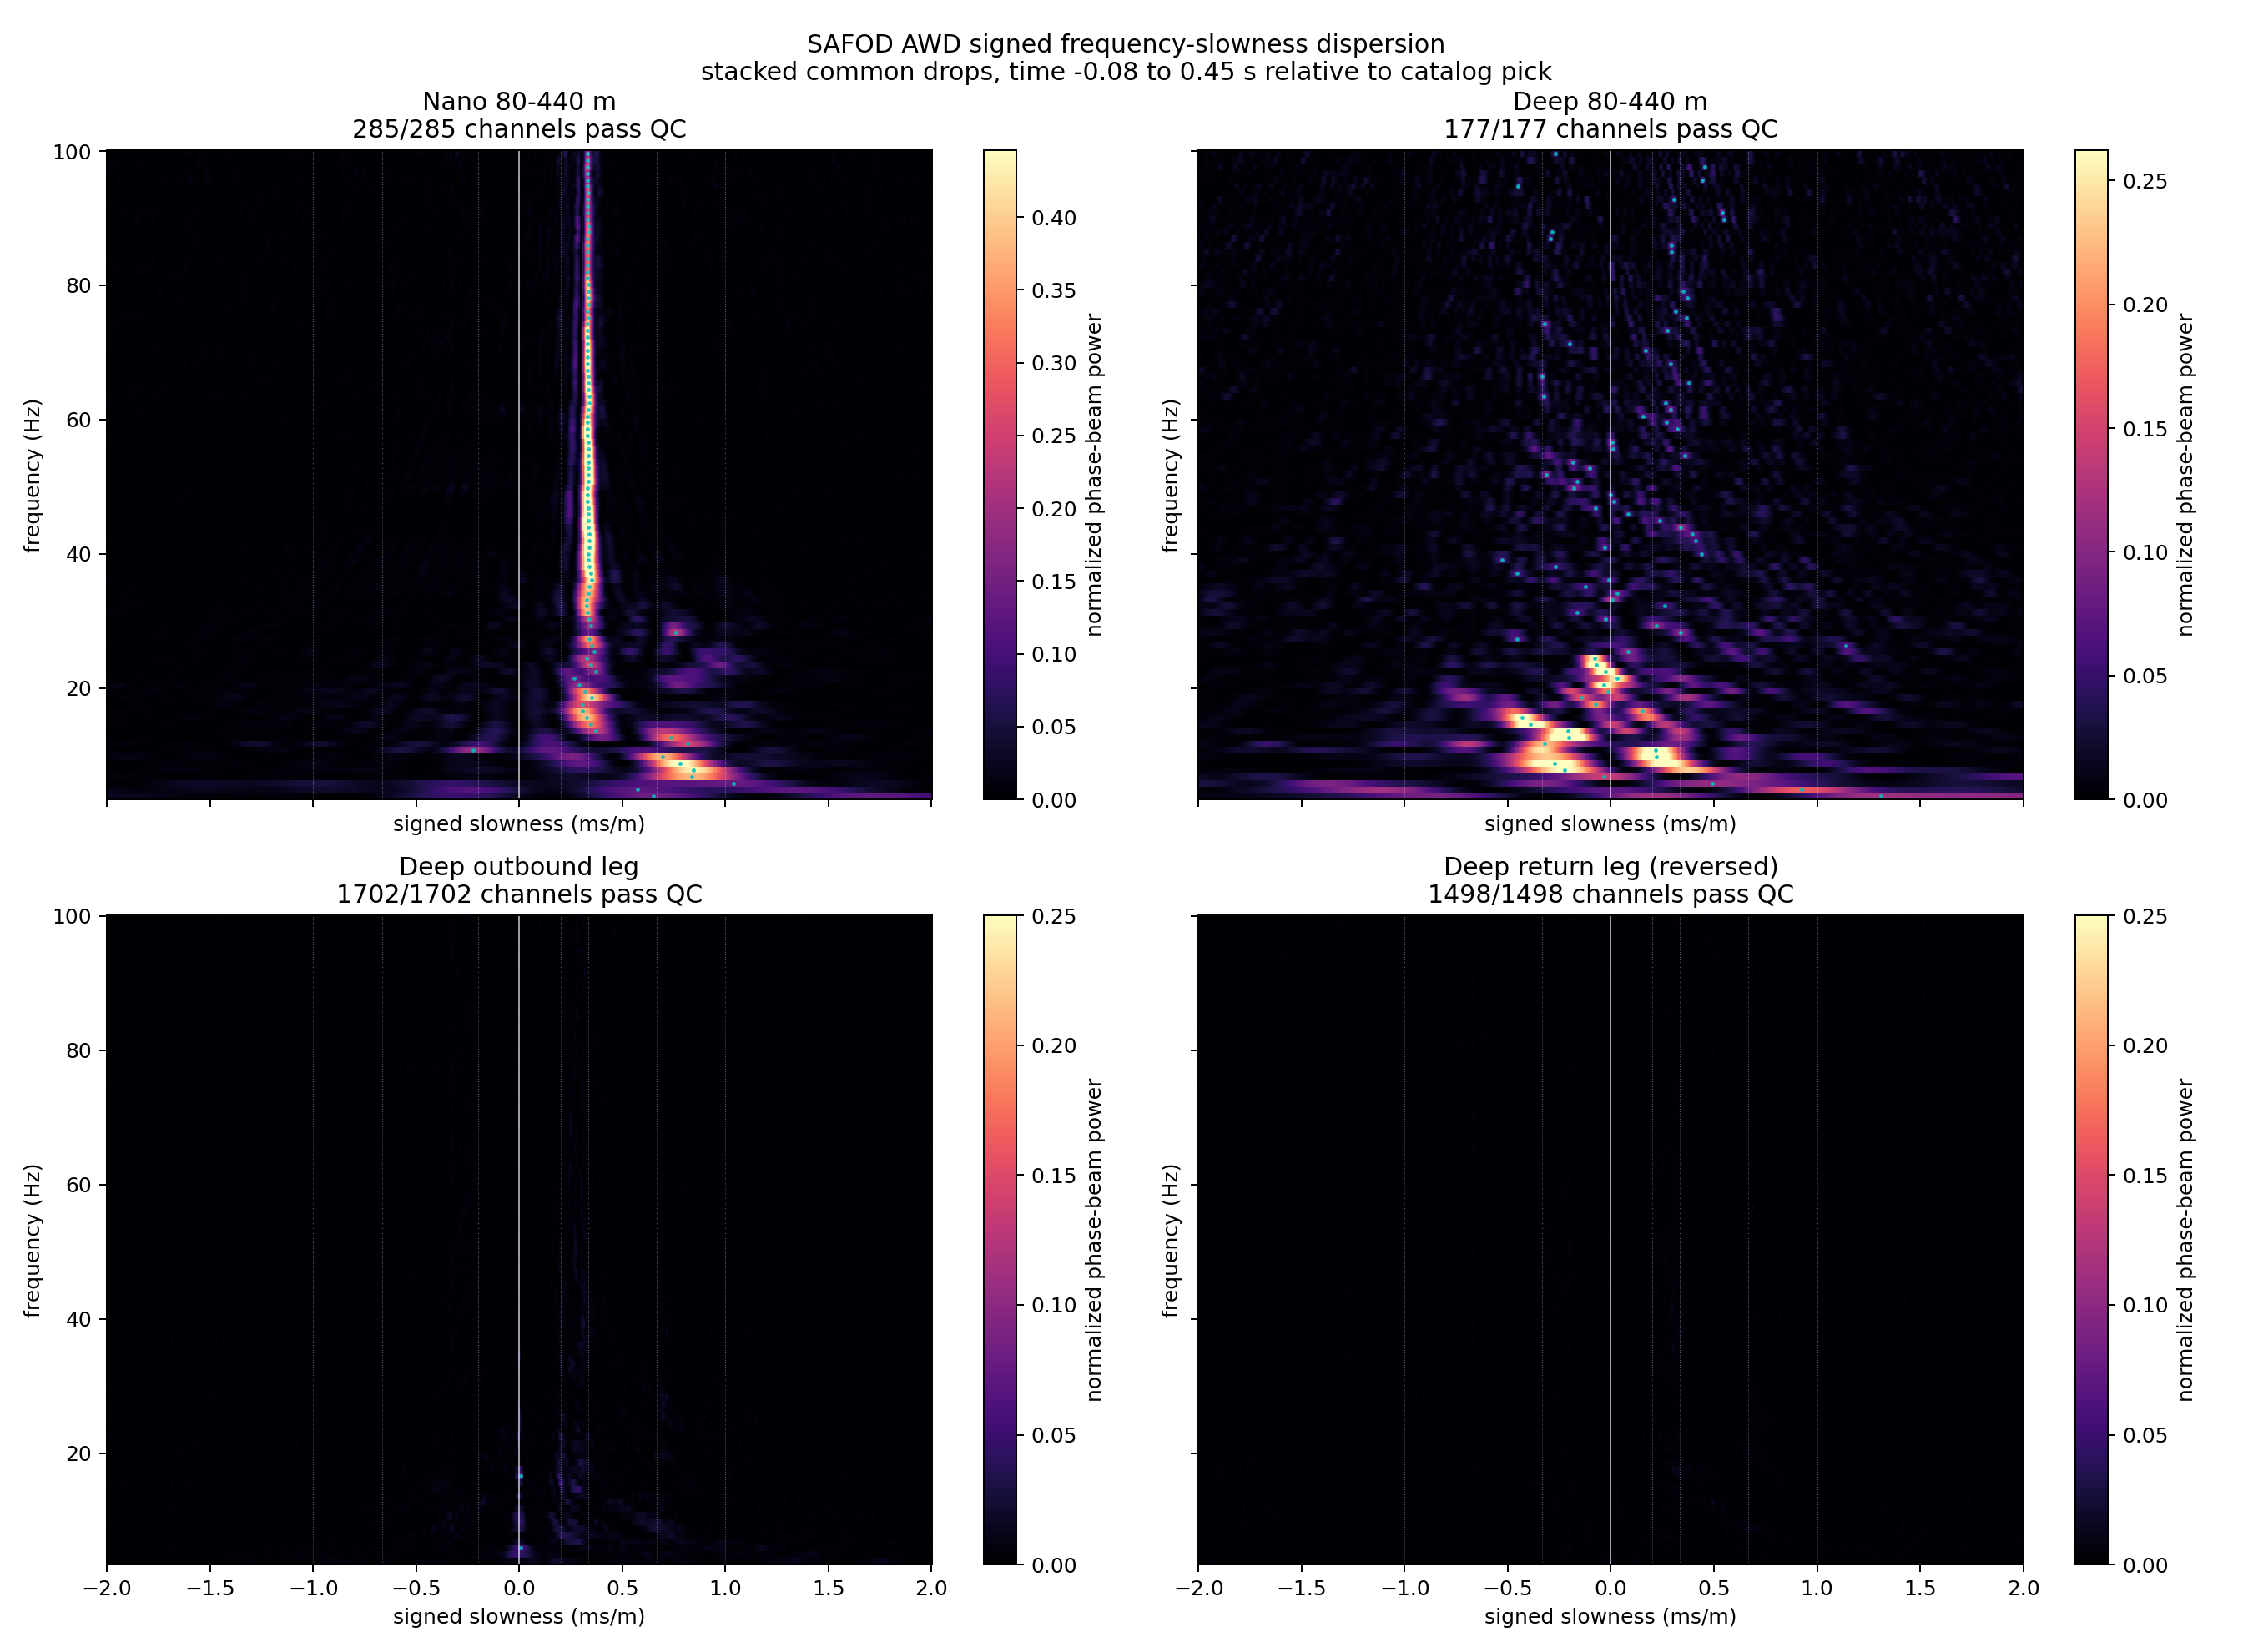
\includegraphics[width=0.90\linewidth]{fk_dispersion.png}
\caption{\textbf{Signed frequency--slowness spectra of the stacked AWD
wavefield.} Panels show Nano over 80--440~m, Deep over the same matched interval,
the complete Deep outbound leg, and the Deep return leg reversed to the same
provisional surface-to-turnaround orientation.  Phase-normalized spatial beams
are evaluated at positive and negative slowness after finite-sample stacking,
detrending, tapering, and channel QC.  The Nano 20--60~Hz ridge has median signed
slowness $+0.335~\mathrm{ms\,m^{-1}}$, equivalent to approximately
$2.985~\mathrm{km\,s^{-1}}$, and positive sign in the displayed coordinate.
The matched Deep interval is weak, while the full Deep legs do not yield a
single stable full-aperture ridge.  The latter result motivates localized
sliding windows; it must not be interpreted as dead-channel failure or proof
that Deep contains no coherent energy.}
\end{figure}

\takeaway{\accepted for Nano: the near-$3~\mathrm{km\,s^{-1}}$ mode has positive
slowness.  \preliminary for Deep: full-leg averaging is a poor representation
of a spatially localized wavefield.}

\subsection{Figure 6: Does Deep contain localized slow modes?}
\figquestion{Can a coherent Deep mode be hidden when the entire hairpin leg is
combined, but become visible in shorter spatial apertures?}

The signed beam is recomputed in overlapping 400~m windows stepped by 200~m.
This sacrifices some slowness resolution but allows mode strength to change
along the borehole.  The search uses lower frequencies and a longer time window
than the shallow Nano analysis because the Deep candidate is slower and travels
farther along fiber.

\begin{figure}[H]
\centering
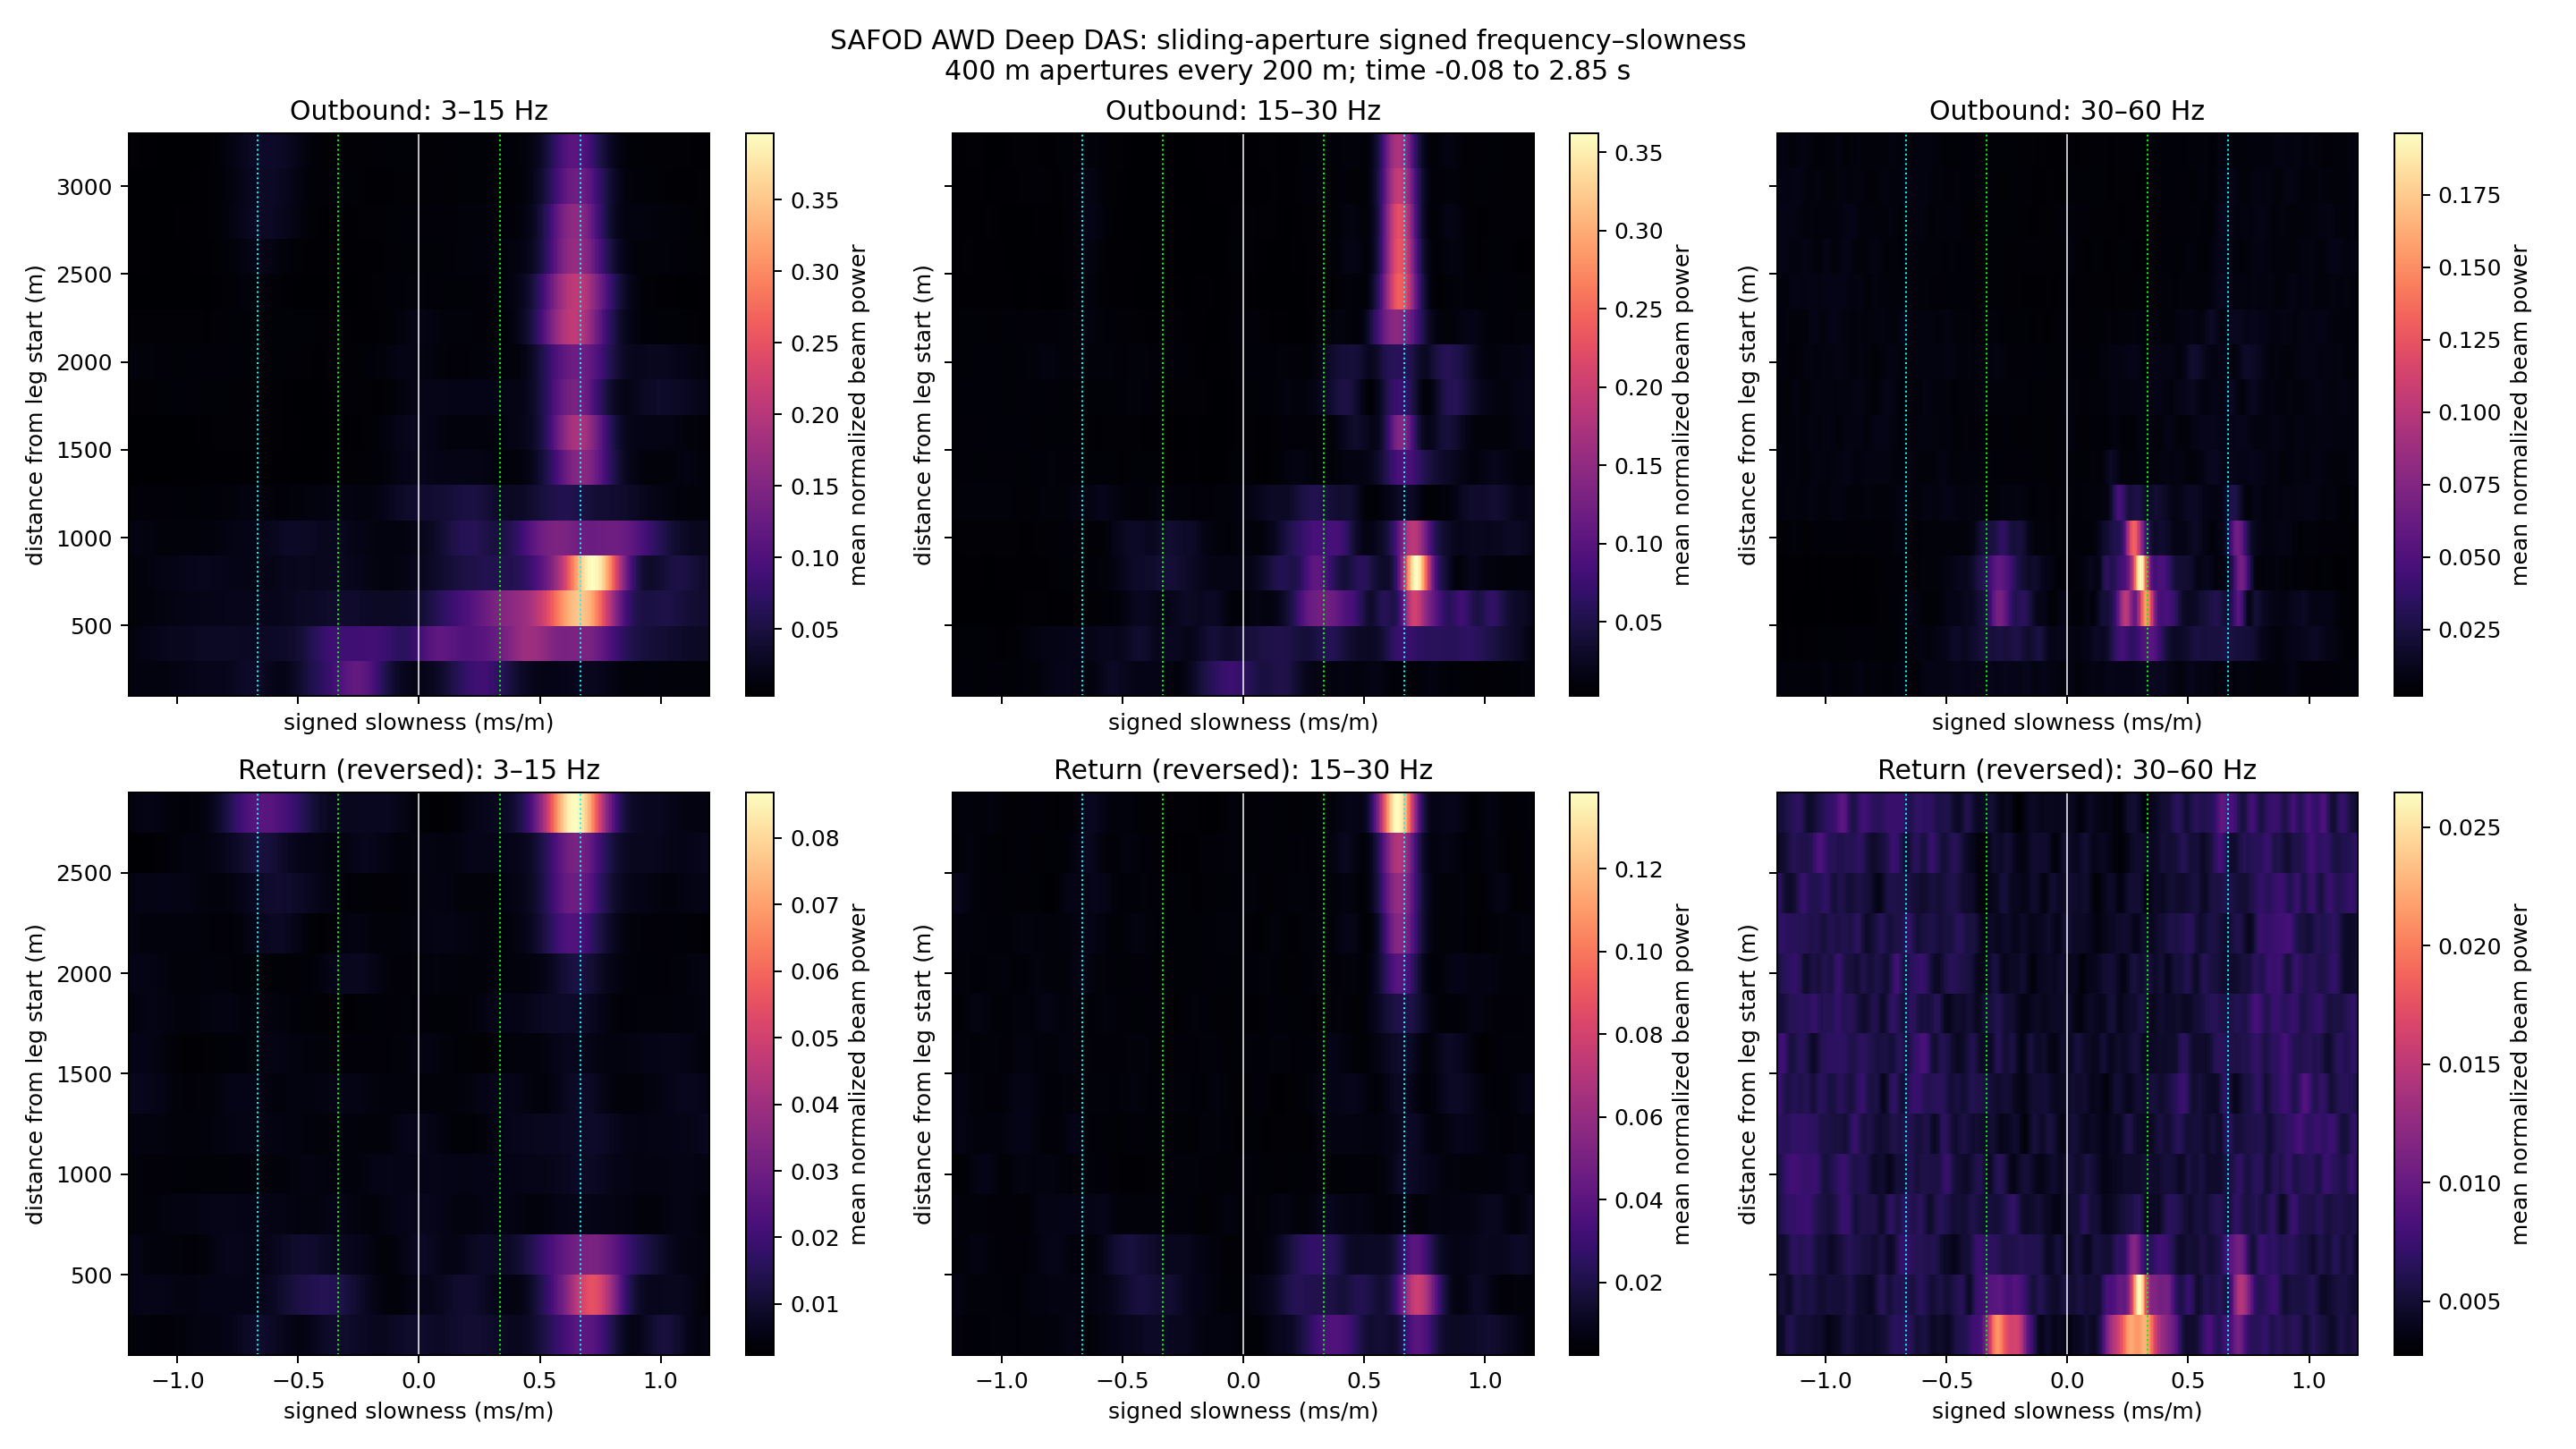
\includegraphics[width=\linewidth]{deep_sliding_fk.png}
\caption{\textbf{Sliding-aperture signed frequency--slowness analysis of the
Deep AWD wavefield.} Rows show outbound and reversed-return legs; columns show
3--15, 15--30, and 30--60~Hz.  Each horizontal slice is a phase-normalized
signed-slowness beam within a 400~m aperture, with neighboring aperture centers
separated by 200~m along the provisional leg coordinate.  A positive-slowness
ridge near $0.64$--$0.72~\mathrm{ms\,m^{-1}}$, corresponding to approximately
$1.4$--$1.56~\mathrm{km\,s^{-1}}$, persists through neighboring apertures on
both legs at 3--30~Hz.  Its slow speed, low-frequency emphasis, and appearance
on a wireline array are compatible with a borehole-guided or tube-wave mode,
but this descriptive all-stack image alone cannot validate repeatability or
assign the physical mode.}
\end{figure}

\takeaway{A coherent slow Deep candidate exists locally.  Its speed is in a
plausible tube-wave range, but physical identification remains preliminary.}

\subsection{Figure 7: What does the Deep candidate look like in time?}
\figquestion{Do independently selected slow-mode trajectories overlay visible
energy in the time domain, and where along each provisional leg are they seen?}

Odd bursts select candidate aperture/slowness combinations.  Their predicted
trajectories are overlaid on a record section made from all common drops.  The
purpose is visual audit: a statistical ridge should correspond to structured
energy in the original coordinate system.

\begin{figure}[H]
\centering
\includegraphics[width=0.91\linewidth]{deep_tube_record_sections.png}
\caption{\textbf{Time-domain expression of the Deep slow-mode candidates.}
Rows show the outbound and reversed-return hairpin legs; columns show 3--15 and
15--30~Hz.  Record sections use the count-weighted stack of 859 complete
same-drop windows in 46 paired bursts and extend from $-0.08$ to $+2.85$~s
relative to code{p26.cc9.txt UTC\_Date}.  Overlaid trajectories were selected
from the odd-burst discovery subset within the positive tube-range slowness
interval rather than tuned to these full-stack images.  Because the Deep axis is
distance from a provisional leg start, and because the time reference is an
arrival-alignment timestamp, the overlays demonstrate time-domain consistency
of a slow coherent mode but do not locate a physical conversion depth.}
\end{figure}

\takeaway{The Deep slow ridge has a time-domain expression and is not only an
$f$--$k$ color-map feature.}

\subsection{Figure 8: Does the Deep slow mode repeat in independent bursts?}
\figquestion{Does a spatial pattern selected with one half of the bursts recur
in a completely independent half?}

Odd-numbered bursts are the discovery sample; even-numbered bursts are the
validation sample.  Discovery chooses six candidate apertures and slownesses
per leg/band.  Validation is evaluated at those fixed choices, preventing the
same data from both selecting and confirming the result.

\begin{figure}[H]
\centering
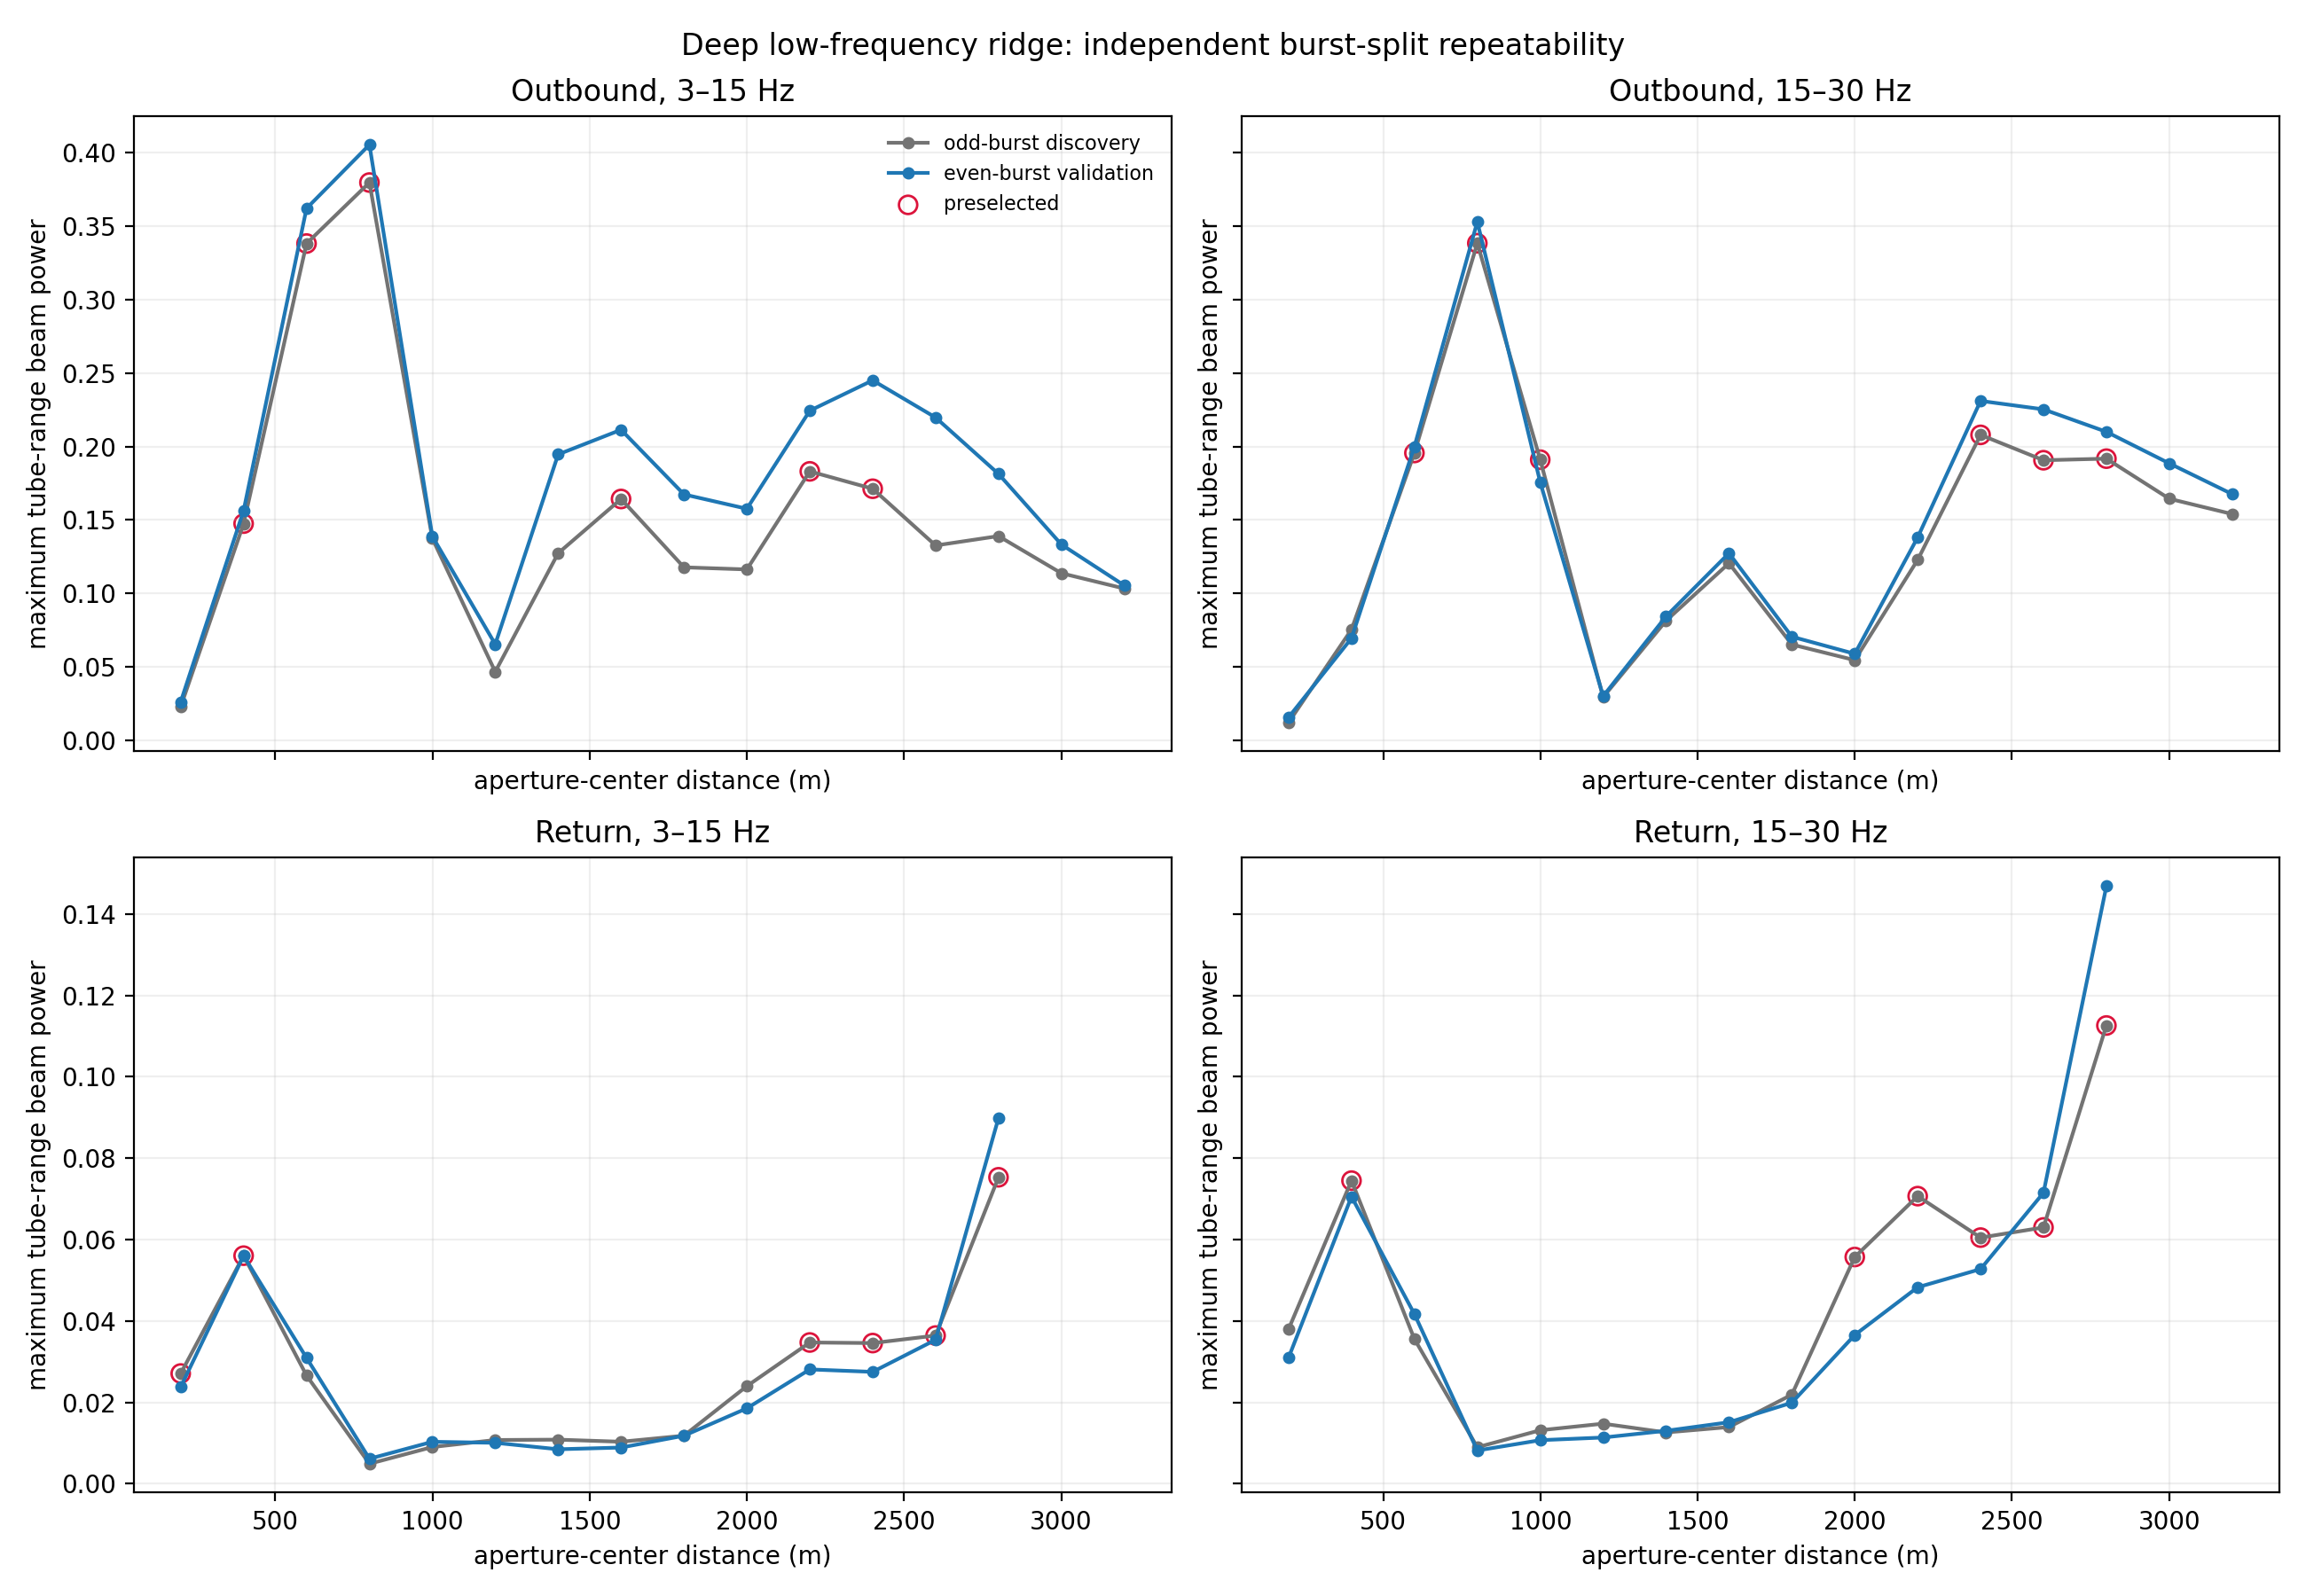
\includegraphics[width=0.91\linewidth]{deep_tube_repeatability.png}
\caption{\textbf{Independent split-sample repeatability of the Deep
positive-slowness mode.} Rows show outbound and reversed-return legs; columns
show 3--15 and 15--30~Hz.  Gray curves are normalized phase-beam power from 23
odd-numbered discovery bursts across overlapping 400~m apertures.  Blue curves
are power from 23 independent even-numbered validation bursts evaluated without
reselecting the target interval.  Candidate apertures and positive slownesses
in the range $0.556$--$0.769~\mathrm{ms\,m^{-1}}$
($1.3$--$1.8~\mathrm{km\,s^{-1}}$) are fixed by discovery.  Agreement of
spatial peaks between the two curves shows that the slow mode is not created
only by stacking every burst or by optimizing one realization.  This validates
repeatability of the spatial mode; the label ``tube wave'' still requires
geometry and borehole-physics corroboration.}
\end{figure}

\takeaway{\accepted: the Deep slow spatial mode repeats in an independent burst
subset.  \preliminary: tube-wave interpretation.}

\subsection{Figure 9: Is the validated Deep pattern stronger than scrambled space?}
\figquestion{At the Deep apertures and slownesses fixed by discovery, can the
validation power be reproduced after destroying channel order?}

This is the Deep analogue of the Nano spatial null, but it preserves the
discovery/validation separation.  The statistic combines fixed predictions;
the permutations are applied only to the validation data.

\begin{figure}[H]
\centering
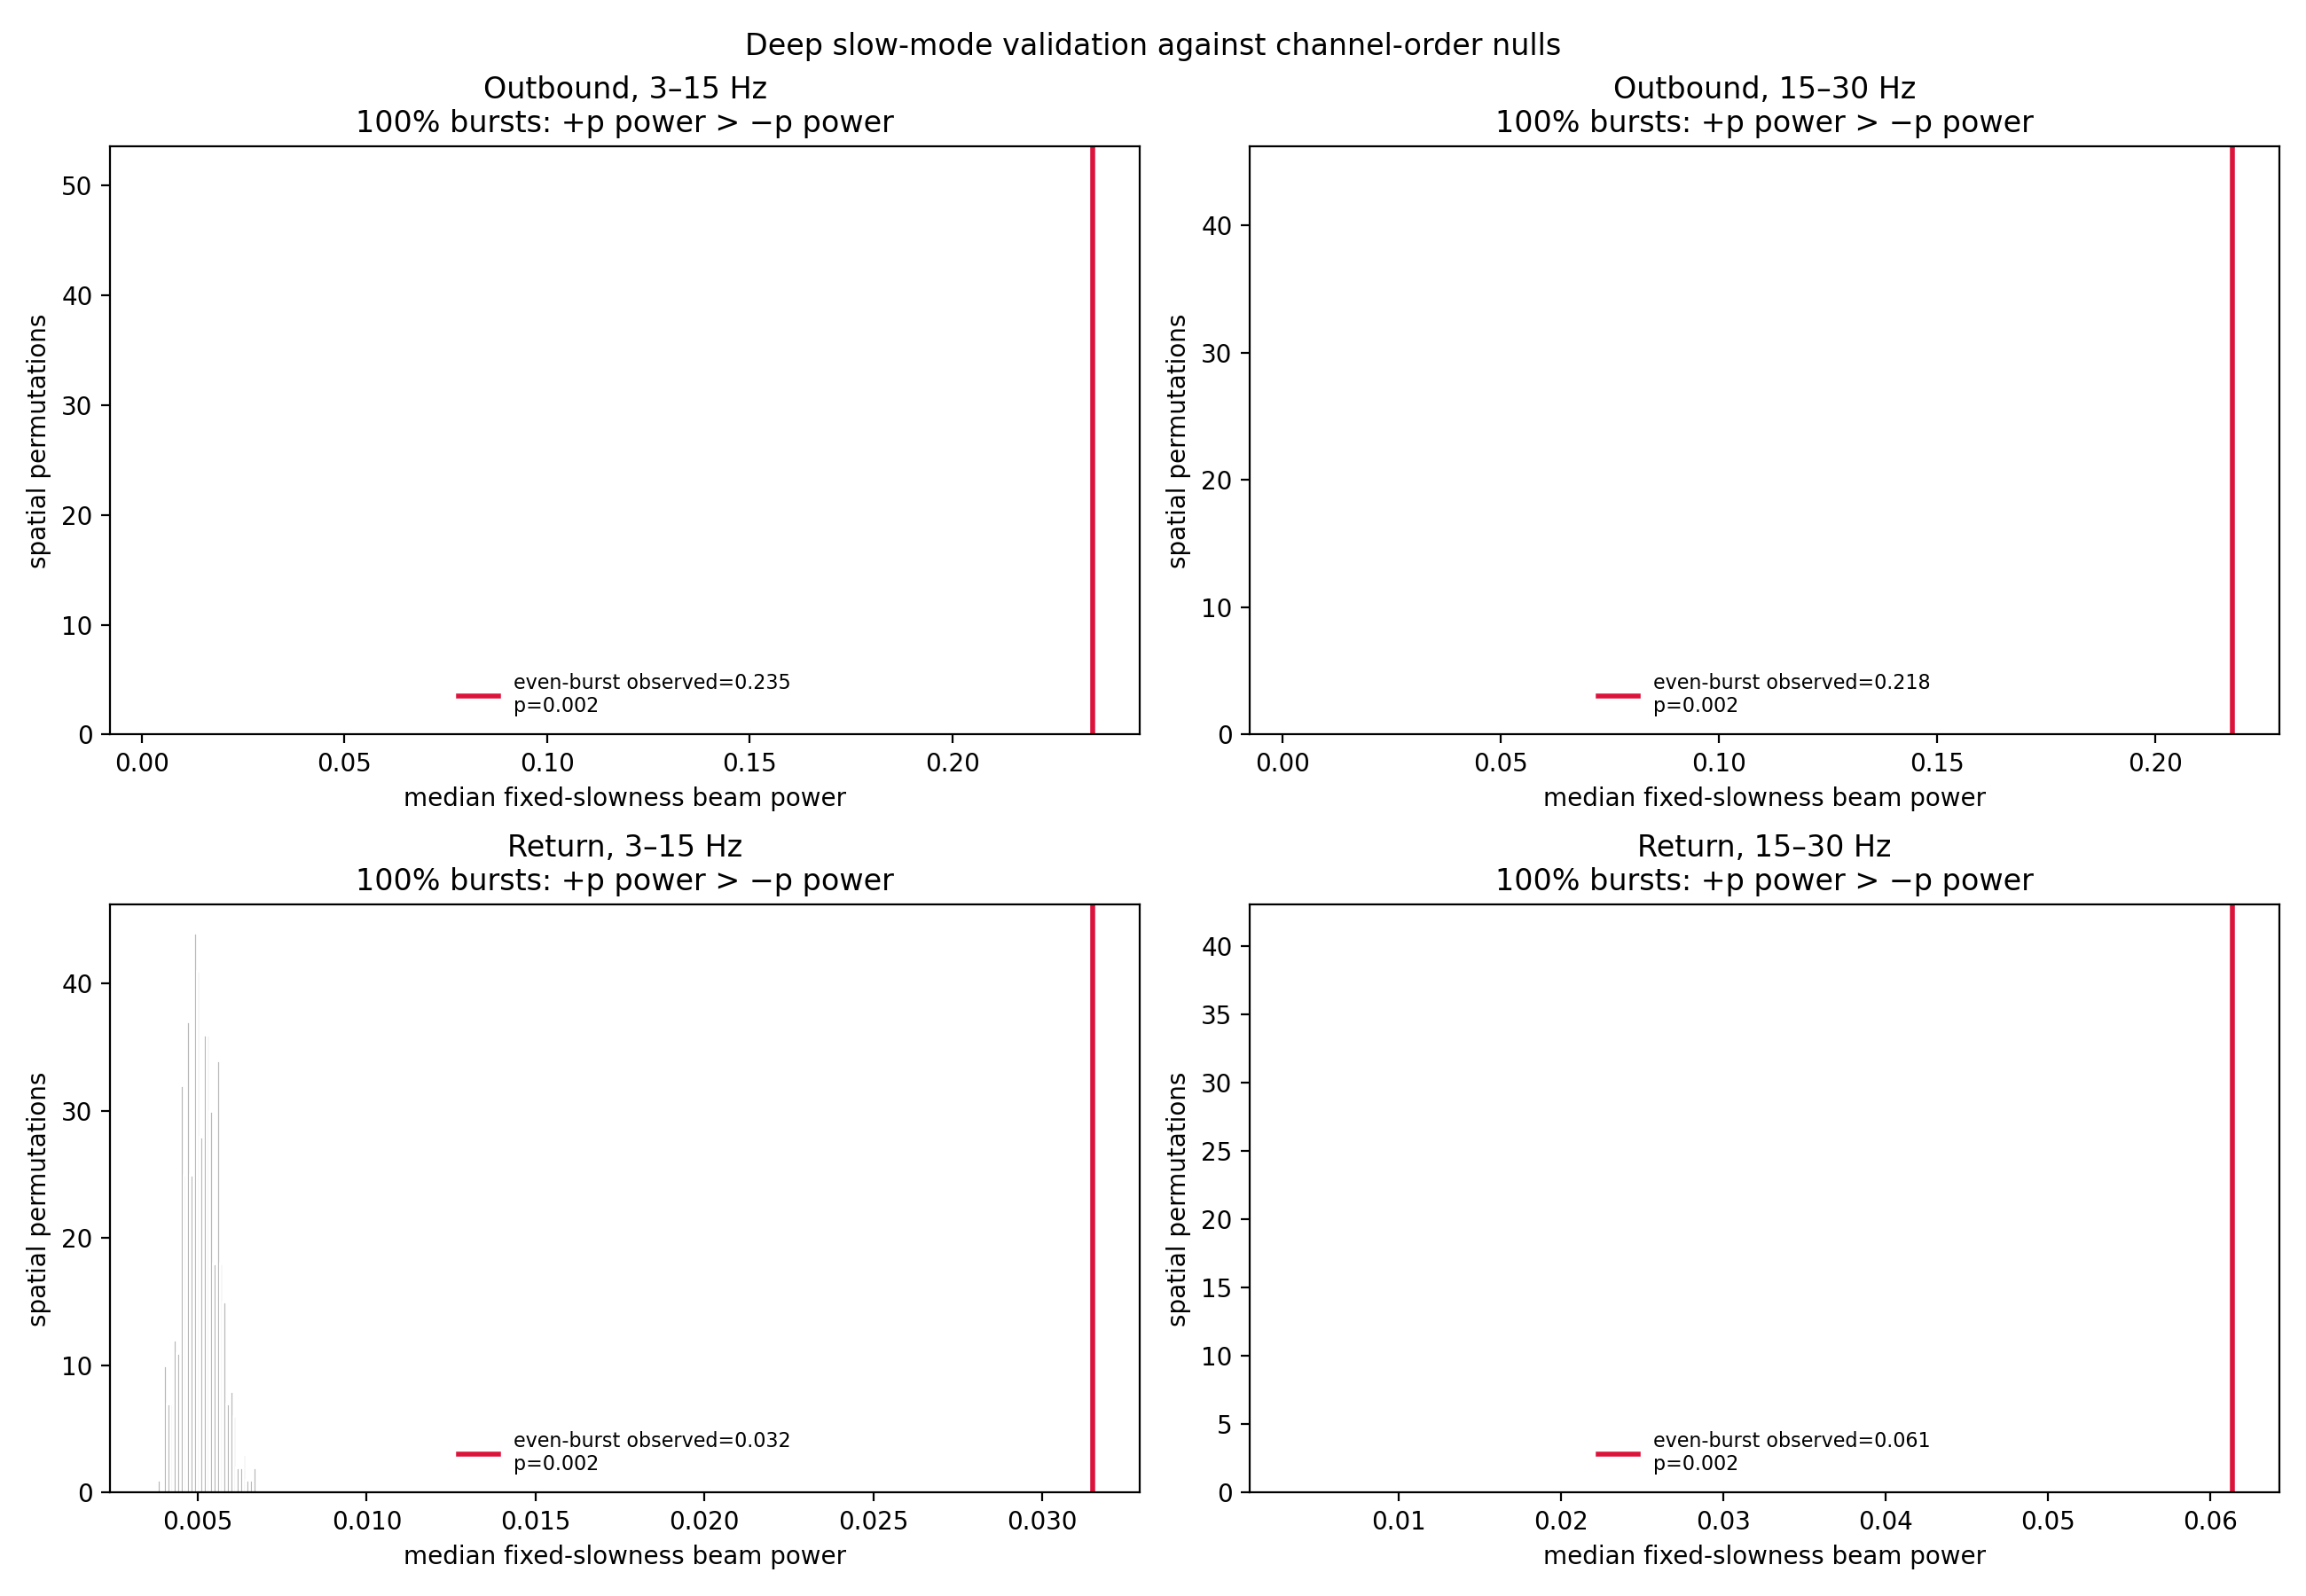
\includegraphics[width=0.91\linewidth]{deep_tube_null_tests.png}
\caption{\textbf{Spatial-order null tests for the fixed Deep slow-mode
predictions.} Panels show both hairpin legs and the 3--15 and 15--30~Hz bands.
The red line is the median even-burst validation power across six apertures and
positive slownesses chosen only from the odd-burst discovery data.  Each gray
histogram contains 499 statistics after independently permuting channel order
within the selected validation apertures while preserving their waveforms and
frequency content.  The unpermuted value exceeds every permutation in all four
leg--band tests, yielding $p=0.002$ in each case.  Moreover, 100\% of individual
bursts have greater power at the fixed positive slowness than at its negative
counterpart.  These observations validate a repeatable, directed slow Deep
mode, but do not by themselves establish fluid pressure, permeability, or a
fracture location.}
\end{figure}

\takeaway{\accepted: the Deep slow mode is statistically significant under the
fixed-prediction spatial null.}

\subsection{Figure 10: Is the Nano mode stable across the experiment?}
\figquestion{Is the near-$3~\mathrm{km\,s^{-1}}$ mode present in individual
burst stacks, or only after averaging the whole experiment?}

Each of the 46 paired bursts receives its own local speed/intercept search near
the all-drop optimum.  Color is coherence, so a stable y-coordinate with weak
color is not equivalent to a precise observation.  Grid increments limit
velocity precision.

\begin{figure}[H]
\centering
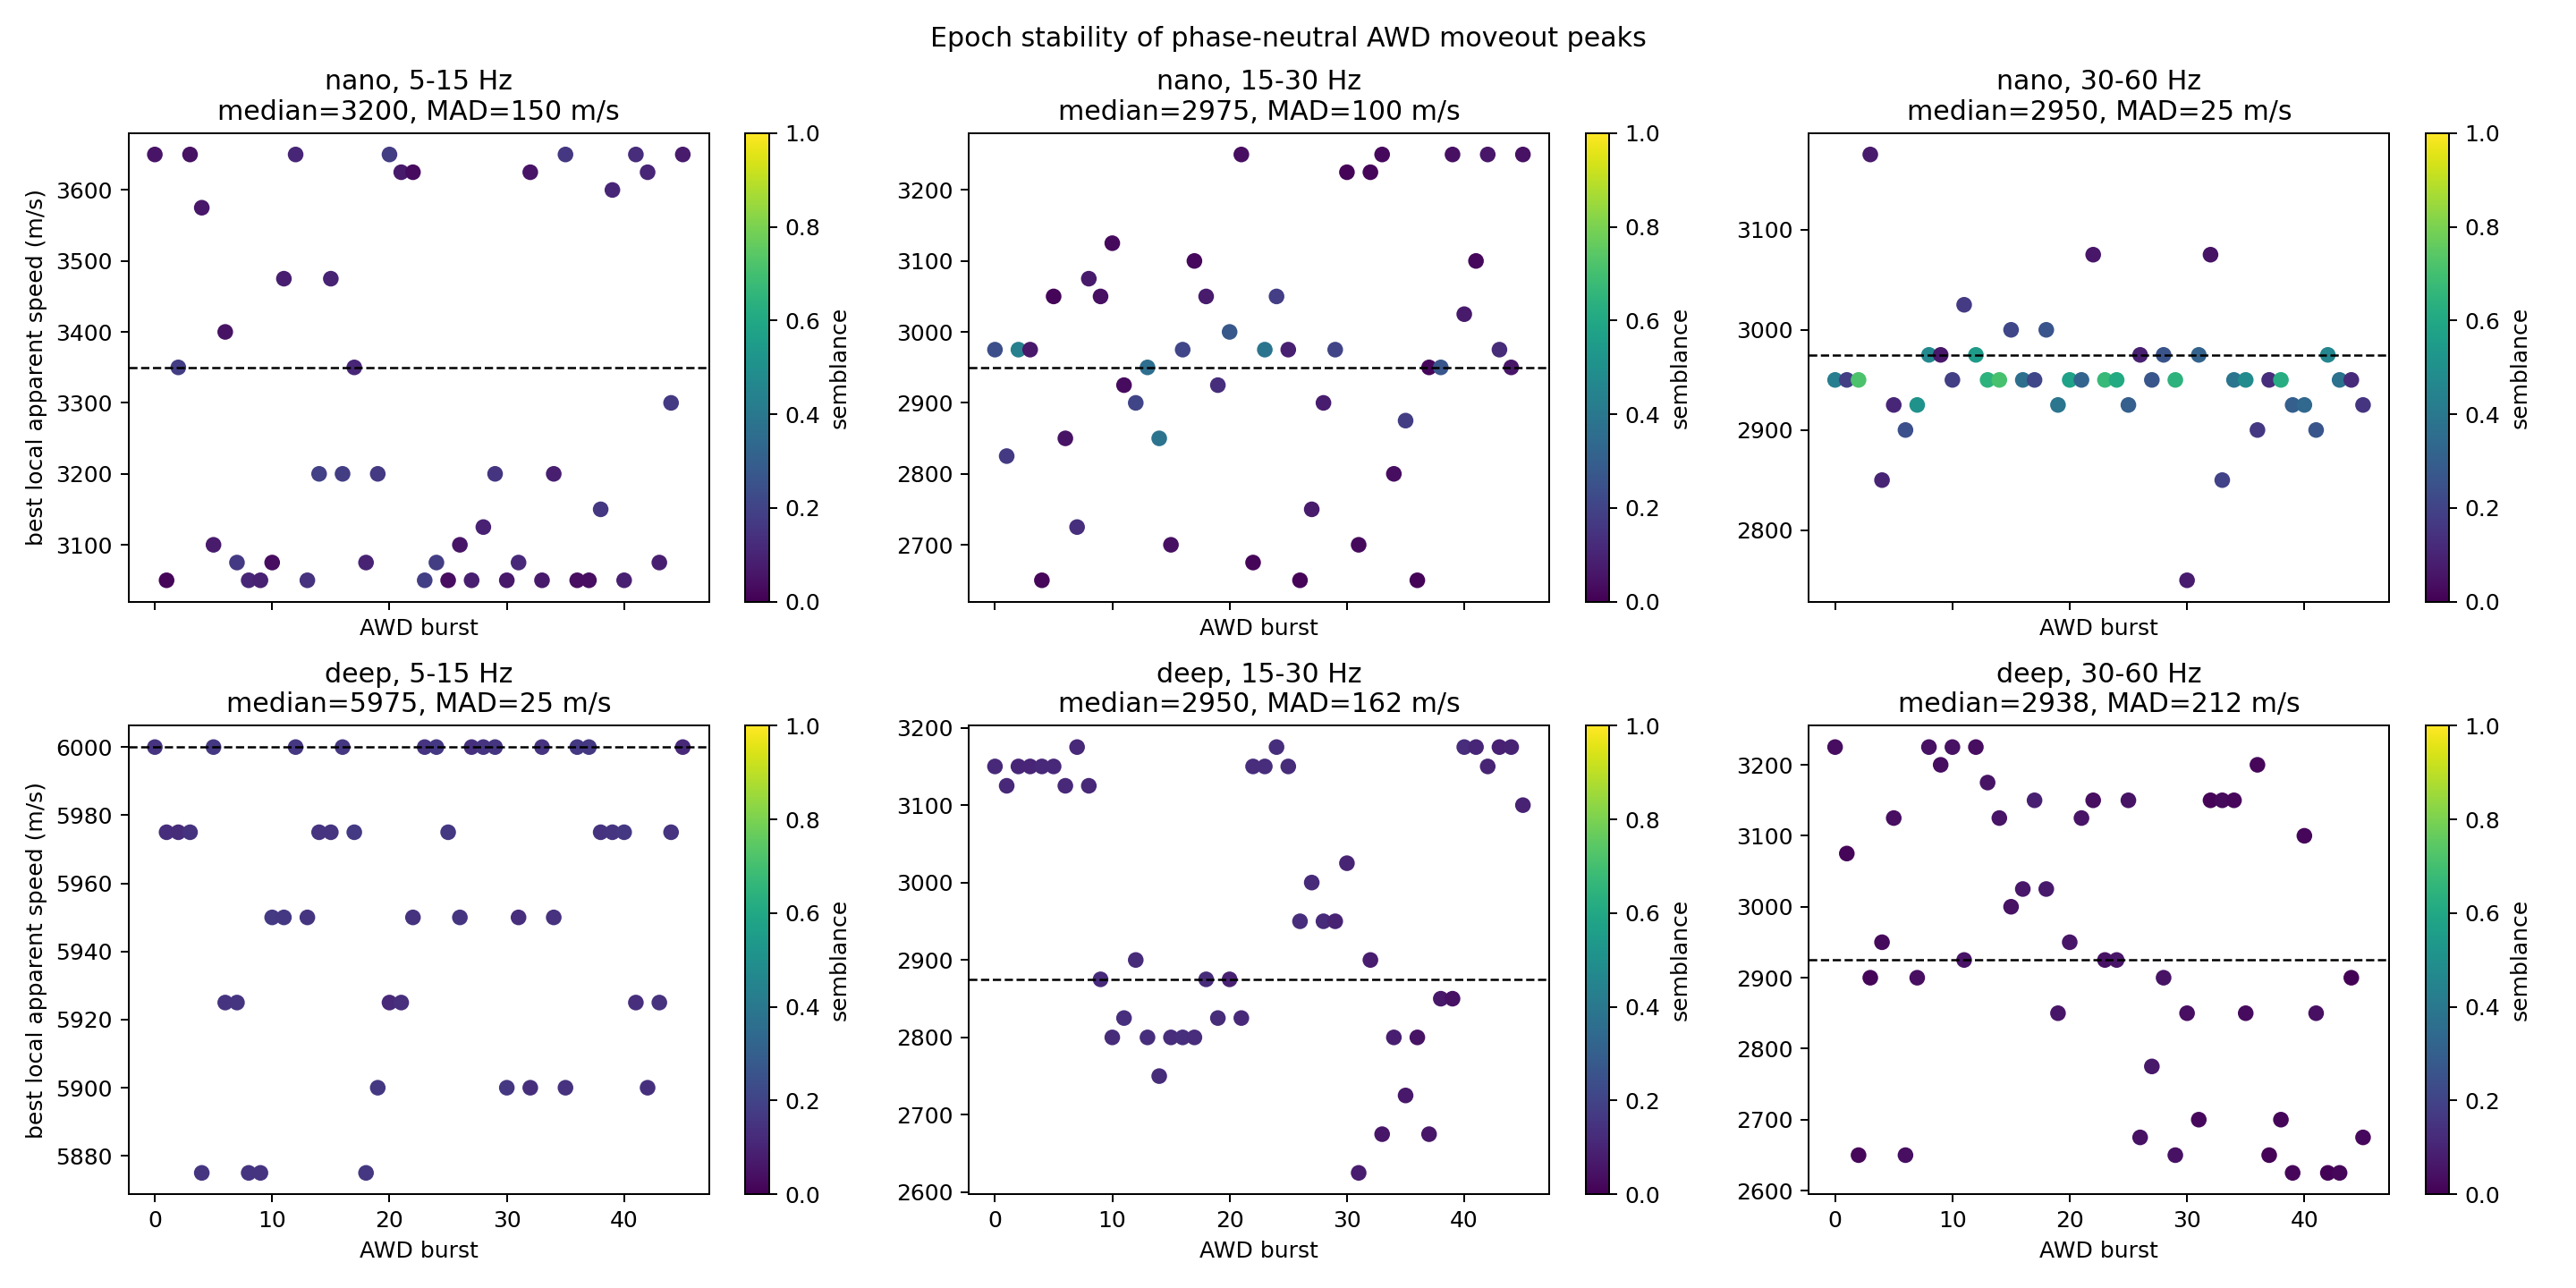
\includegraphics[width=\linewidth]{mode_repeatability.png}
\caption{\textbf{Burst-to-burst stability of phase-neutral apparent-speed
estimates.} Rows compare Nano and matched-aperture Deep data; columns show
5--15, 15--30, and 30--60~Hz.  Each point is one paired burst, its vertical
position is the locally optimal apparent speed, and color is the associated
semblance on a common 0--1 scale.  The dashed line is the all-burst reference;
each burst is searched within $\pm300~\mathrm{m\,s^{-1}}$ and $\pm20$~ms of that
reference.  Nano 30--60~Hz estimates cluster near a mean of
$2.952~\mathrm{km\,s^{-1}}$, with 30 of 46 bursts exceeding semblance 0.2.
The lower-frequency Nano mode is weaker, while the matched shallow Deep
aperture does not reproduce the Nano pattern.  Scatter at or below the scan-grid
increment must not be interpreted as physical velocity precision.}
\end{figure}

\takeaway{\accepted at burst scale: the strongest Nano mode is not solely a
full-stack phenomenon.  The completed within-burst and individual-drop hierarchy
is quantified in Figure 12 and supplies the source-repeatability uncertainty.}

\subsection{Figure 11: Which frequencies are useful, and how far do they reach?}
\figquestion{At what frequencies and fiber positions does the Nano AWD signal
remain stronger than pre-reference noise?}

Signal windows follow the accepted moveout trajectory.  Equal-duration noise
windows precede the reference time.  Spectra are stabilized by multitaper
estimation and local channel averaging.  The figure measures an empirical
monitoring aperture, not attenuation alone: geometric spreading, coupling,
noise, interference, and instrument response all contribute.

\begin{figure}[H]
\centering
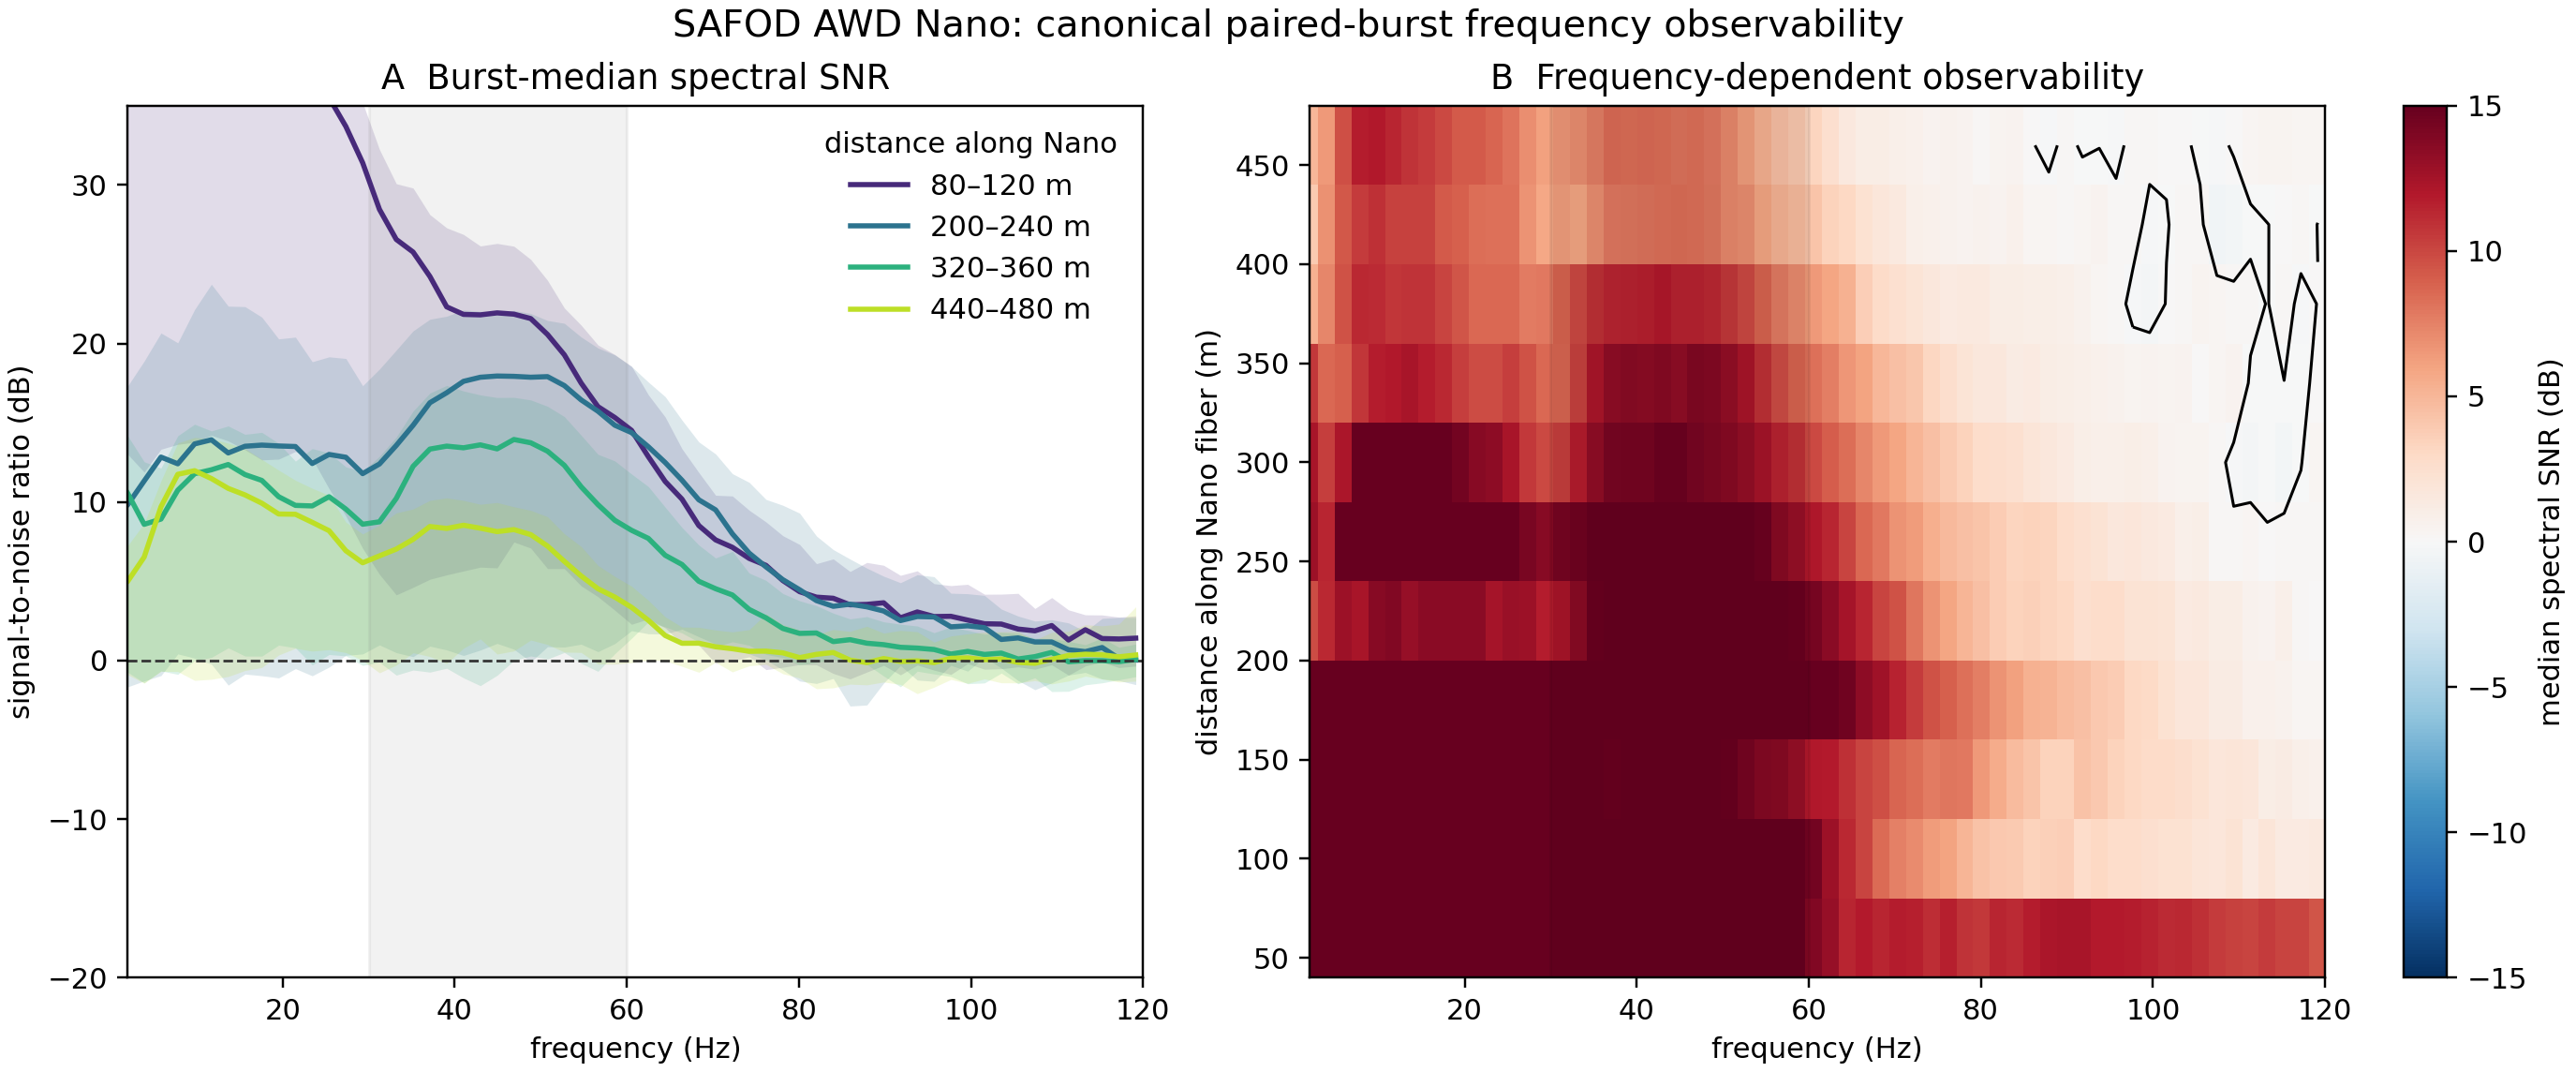
\includegraphics[width=\linewidth]{nano_frequency_observability.png}
\caption{\textbf{Frequency-dependent observability of the canonical Nano AWD
signal relative to pre-reference noise.} Signal spectra are measured in 0.24~s
windows following the phase-neutral trajectory
$t=-0.022~\mathrm{s}+x/(2{,}975~\mathrm{m\,s^{-1}})$; noise spectra use
equal-duration windows from $-0.38$ to $-0.14$~s.  Spectra are estimated for
each of 46 complete paired burst stacks using four discrete-prolate-spheroidal
tapers and are averaged within 40~m fiber-coordinate bins before forming SNR.
The panels summarize representative distances and the along-fiber behavior of
the 30--60~Hz band.  Median 30--60~Hz SNR declines from approximately 21.8~dB
at the 100~m bin to 7.6~dB at the 460~m bin and remains above 0~dB through the
farthest tested 460~m bin.  This supports a usable canonical-stack monitoring
aperture through that bin; it does not show that every individual drop is
detectable there.}
\end{figure}

\takeaway{\accepted for burst stacks: 30--60~Hz is the principal Nano monitoring
band, with positive median spectral SNR through the 460~m bin.}

\subsection{Supplemental diagnostic: What does stacking actually contribute?}
\figquestion{Can the relevant Nano and Deep modes be seen in one drop, how much
does a burst stack help, and what additional structure appears only in the full
experiment stack?}

This figure uses one objectively selected representative drop: the temporal
center of the burst with the most paired drops.  It then shows the associated
single drop, the 21-drop burst mean, and the 859-drop weighted mean with the
same noise-RMS display scale within each installation.  This is a visualization
of scale; the quantitative hierarchical individual-drop repeatability result is provided in Figure 12.

\begin{figure}[H]
\centering
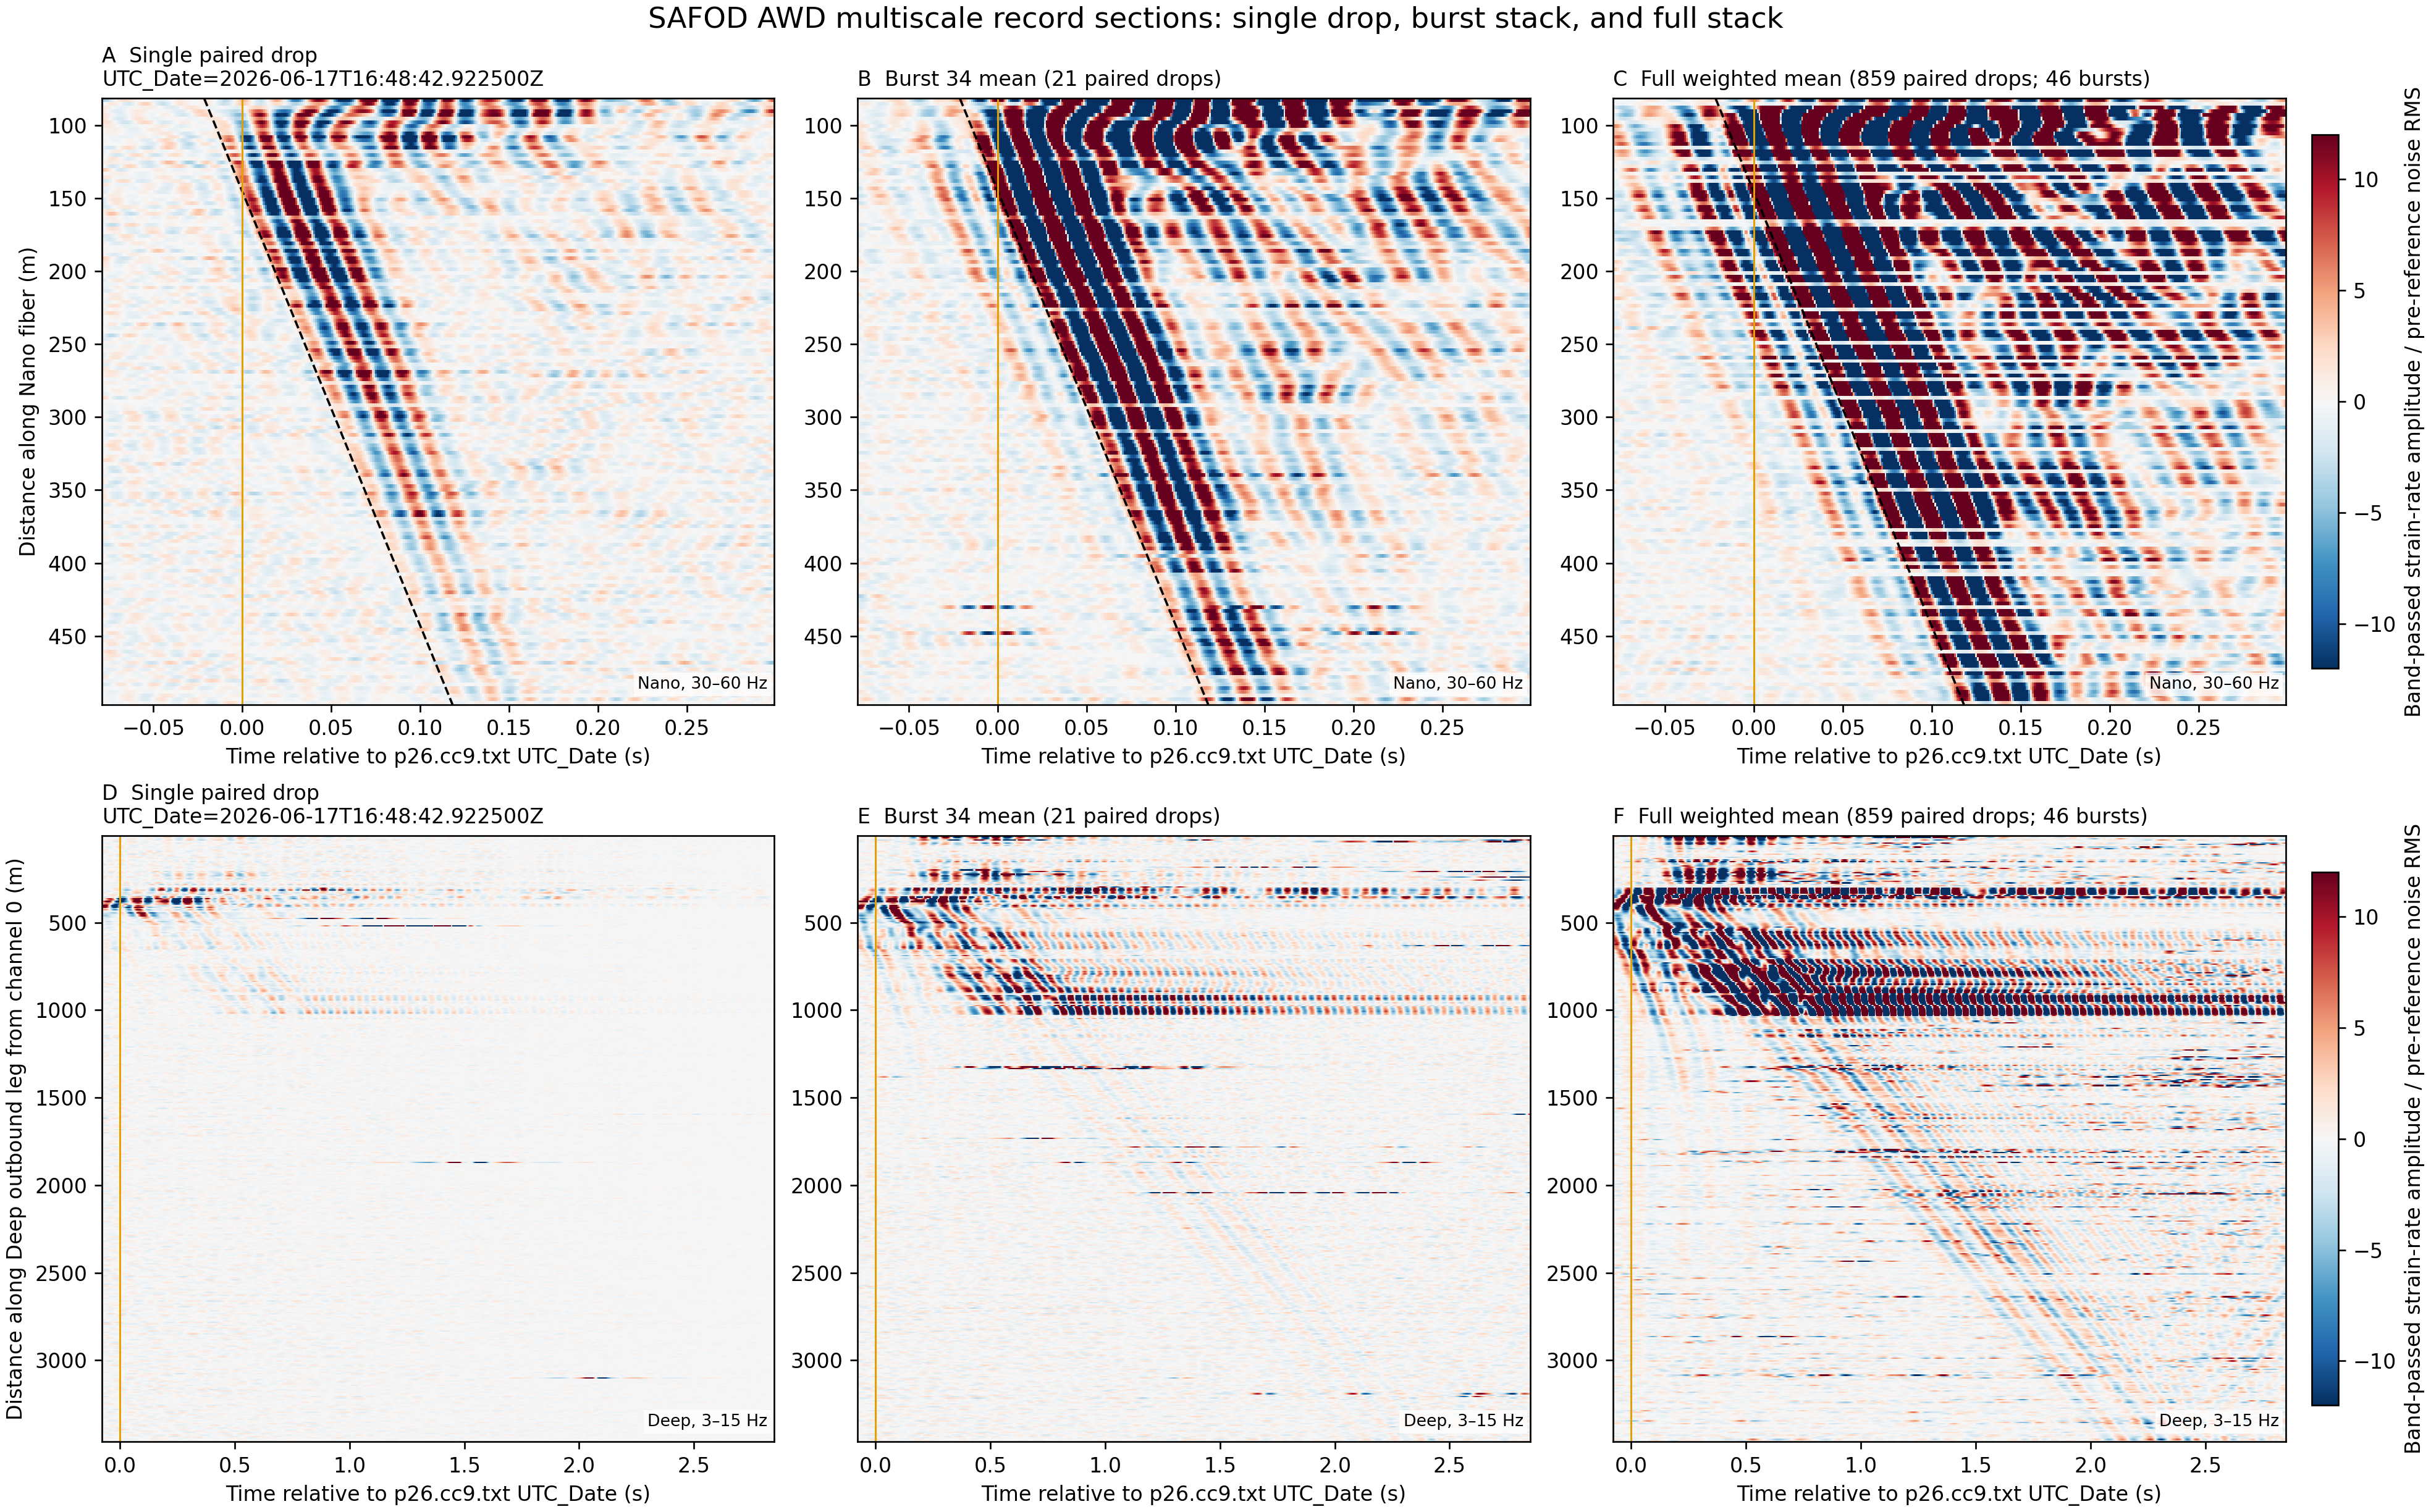
\includegraphics[width=\linewidth]{awd_multiscale_record_sections.png}
\caption{\textbf{AWD record sections at single-drop, burst, and experiment
scales.} Columns show one paired drop, its 21-drop burst mean (burst 34), and the
count-weighted mean of 859 paired drops from 46 bursts.  The selected event is
the temporal center of the burst with the greatest paired-drop count, avoiding
manual selection for an unusually clear waveform.  The top row shows cemented
Nano data at 30--60~Hz over 80--500~m; the bottom row shows the wireline Deep
outbound leg at 3--15~Hz over 0--3473.3~m along provisional fiber coordinate.
Every trace is divided by its RMS amplitude in the common $-0.45$ to $-0.15$~s
pre-reference interval, and every panel uses fixed limits of $\pm12$ noise RMS.
The orange line marks code{p26.cc9.txt UTC\_Date}; the dashed Nano overlay is
the accepted $2.975~\mathrm{km\,s^{-1}}$ apparent-moveout trajectory.  Differences
from left to right show the visibility gained by stacking while preserving a
common amplitude convention.  The figure demonstrates whether representative
single-event structure exists, but one selected drop cannot quantify the full
within- and across-burst distribution.}
\end{figure}

\takeaway{Completed diagnostic: stacking visibly improves coherent structure.
The quantitative hierarchical repeatability analysis is now also complete: 988
drops from 49 bursts were tested, signal NCC exceeded the equal-duration noise
NCC in all 49 bursts, and leave-one-burst-out burst-template NCC had median
0.976.  Figure 12 is the quantitative companion to this multiscale display.}

\subsection{Supplemental diagnostic: Is the Nano mode dispersive?}
\figquestion{Does the coherent Nano trajectory have the same apparent slowness
at every frequency, and is its positive direction supported burst by burst?}

Five frequency bands are fit independently.  Bursts, not channels, are
bootstrap resampling units, so the uncertainty represents experiment-to-
experiment burst variability more honestly than treating thousands of samples
as independent.  The analysis estimates a coherent-window trajectory, not an
onset pick.

\begin{figure}[H]
\centering
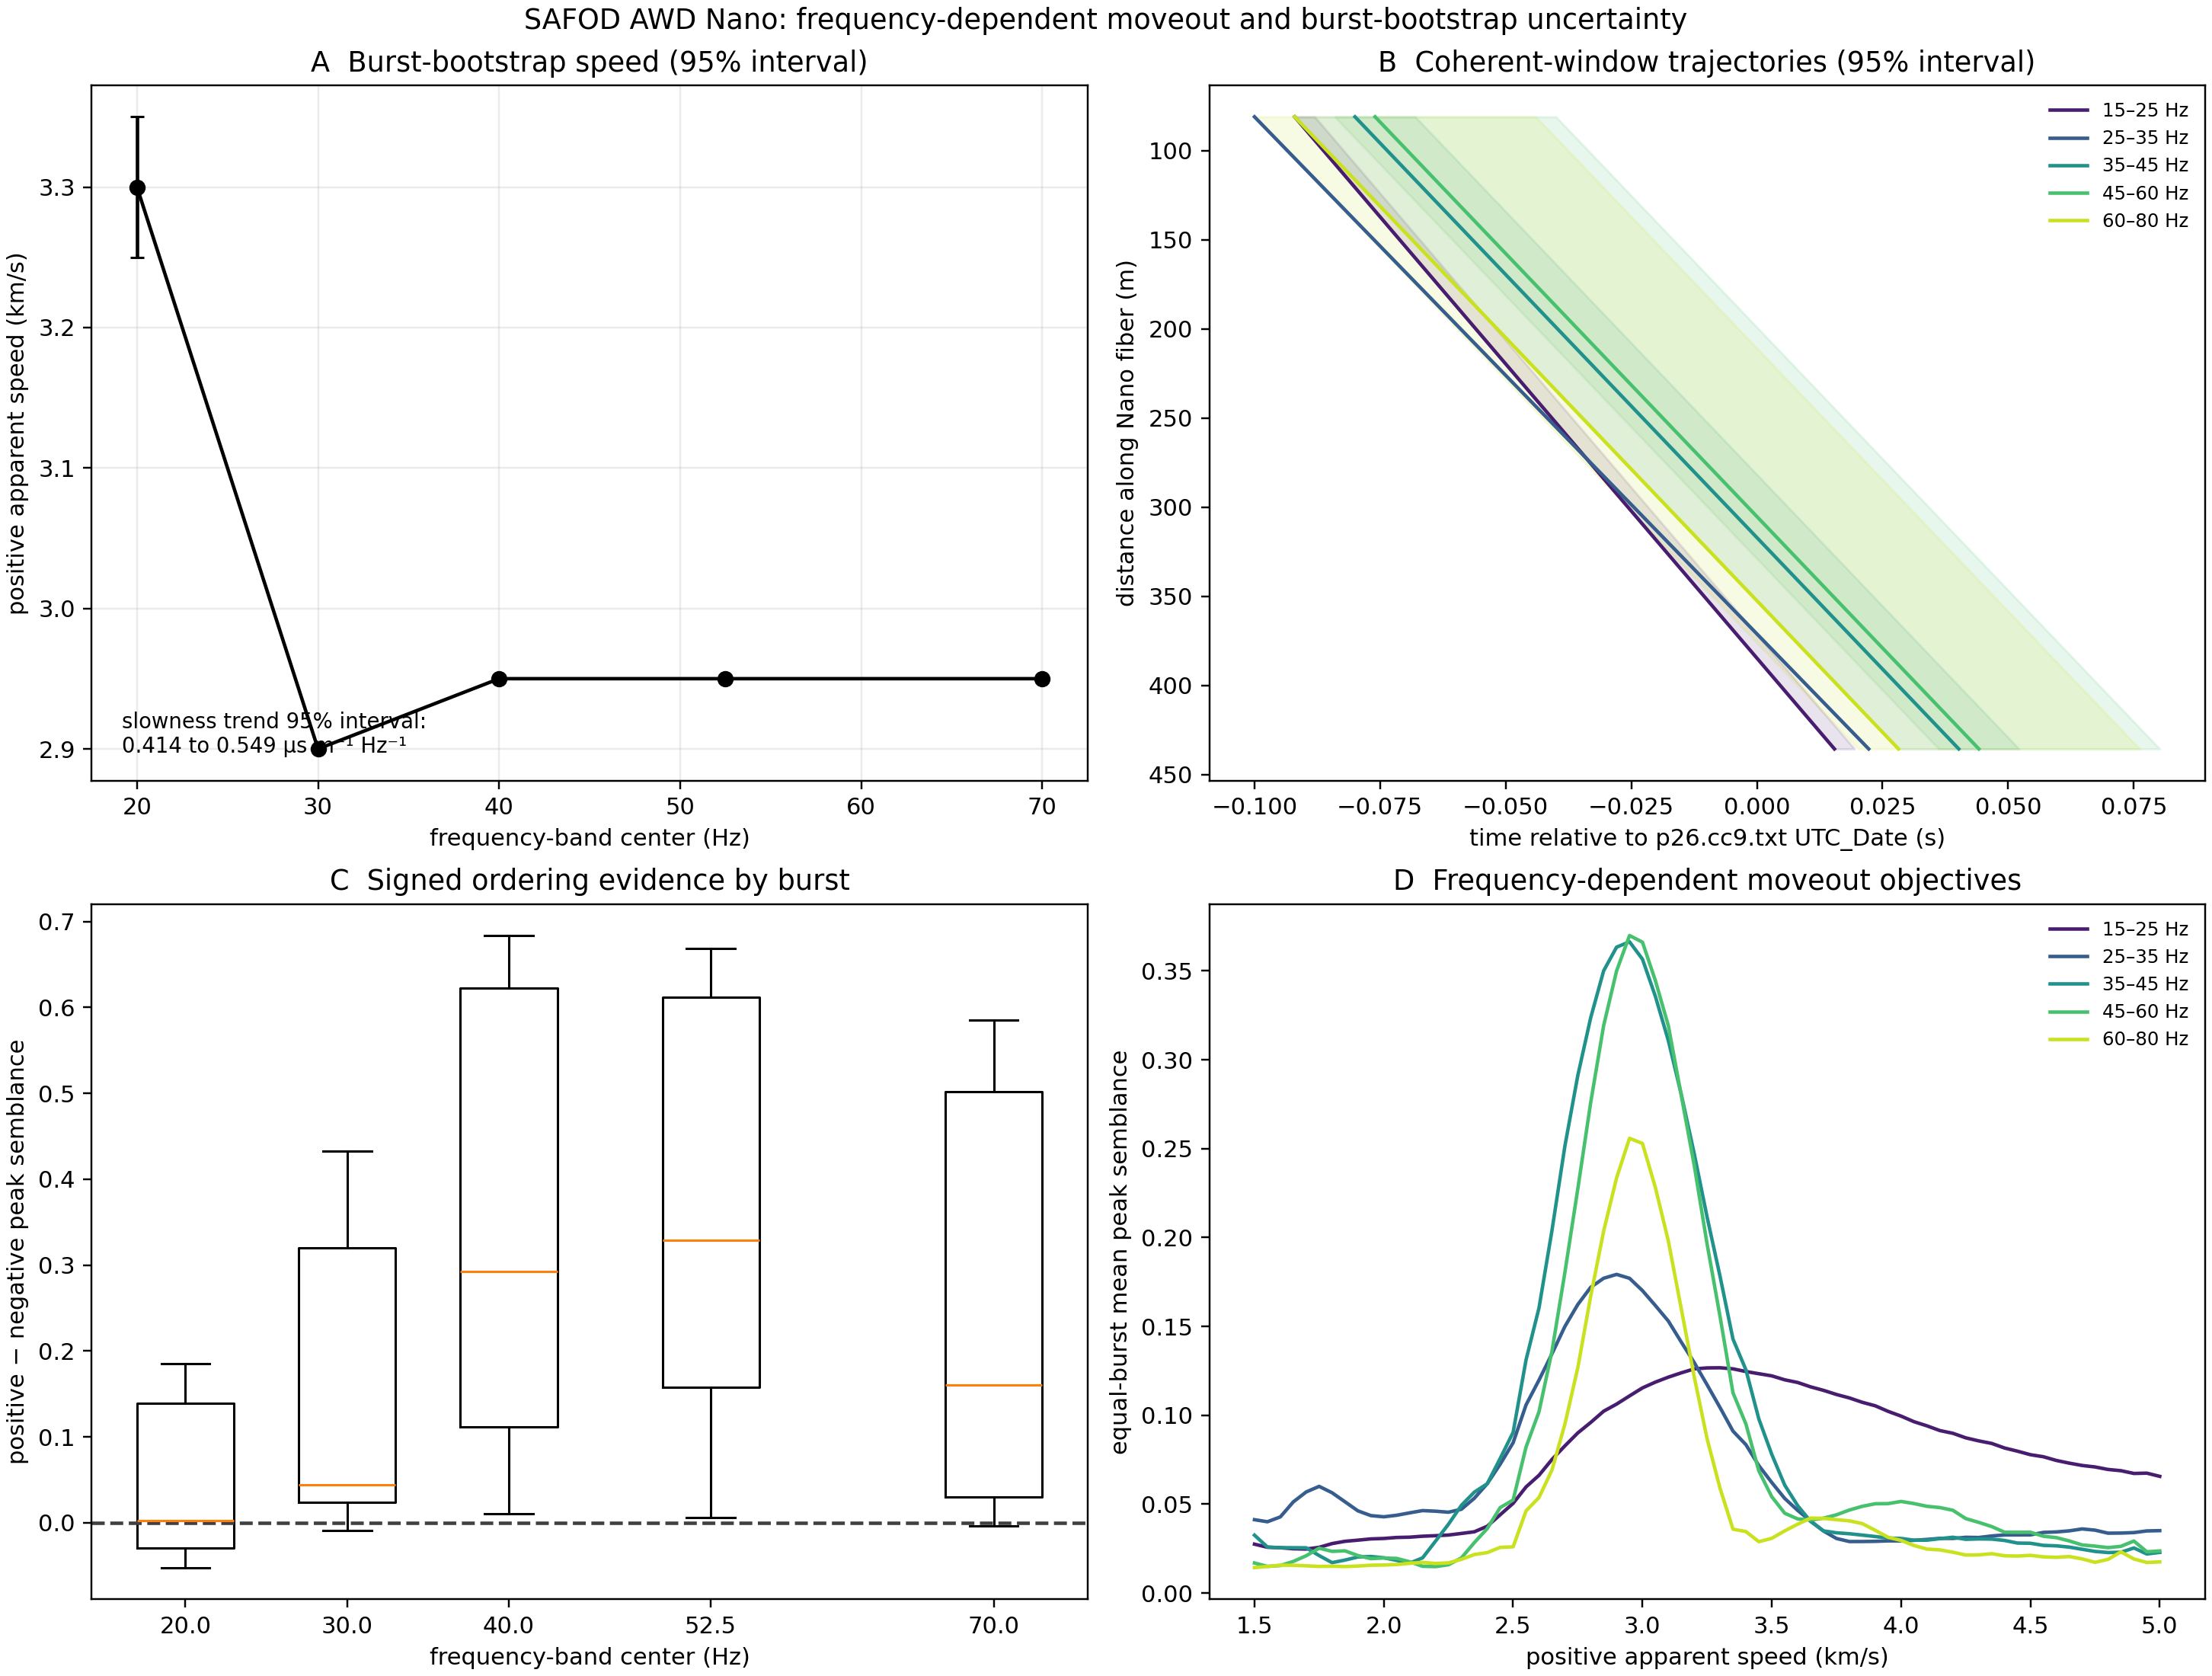
\includegraphics[width=0.91\linewidth]{nano_mode_identification.png}
\caption{\textbf{Frequency-dependent Nano moveout and burst-bootstrap
uncertainty.} (a) Positive apparent speed in five bands from 15 to 80~Hz; points
are burst-bootstrap medians and bars are 95\% intervals from 999 resamples of
46 bursts representing 859 common drops.  (b) Corresponding coherent-window
trajectories across the Nano aperture; shaded regions show bootstrap intervals,
and the plotted $t_0$ is the coherence-window start at the first aperture
channel rather than a physical phase pick.  (c) Distribution across bursts of
the difference between the best positive- and negative-slowness coherence;
values above zero favor the observed positive ordering.  (d) Equal-burst mean
moveout objective versus positive apparent speed in each band.  Median speeds
are approximately 3.30~km~s$^{-1}$ at 15--25~Hz, 2.90~km~s$^{-1}$ at
25--35~Hz, and 2.95~km~s$^{-1}$ from 35 to 80~Hz.  Every band favors positive
ordering with bootstrap probability 1.0.  The bootstrap interval for the
frequency trend in slowness is positive (0.414--0.549~$\mu$s~m$^{-1}$~Hz$^{-1}$),
so a monotonic frequency dependence is resolved under this estimator.  Such
dispersion is compatible with guided/coupled propagation but is not unique to
it; the test alone cannot distinguish direct P from a weakly dispersive guided
mode.}
\end{figure}

\takeaway{\accepted as an empirical mode property: positive ordering is robust
and frequency-dependent slowness is resolved.  Physical phase identity remains
unresolved, so the approximately 3~km~s$^{-1}$ value is not yet a $V_P$ profile.}

\subsection{Supplemental diagnostic: Do opposite Deep branches locate a conversion depth?}
\figquestion{Can independently validated upgoing- and downgoing-sign candidates
be paired to identify a fixed generation or reflection coordinate?}

Time gates are selected with odd bursts and scored with even bursts.  A purely
geometric intersection is not sufficient; the joint feature must also exceed a
spatial-order null.  Markers show candidates even when they fail the final
test, so an empty set of significant stars is a real negative result.

\begin{figure}[H]
\centering
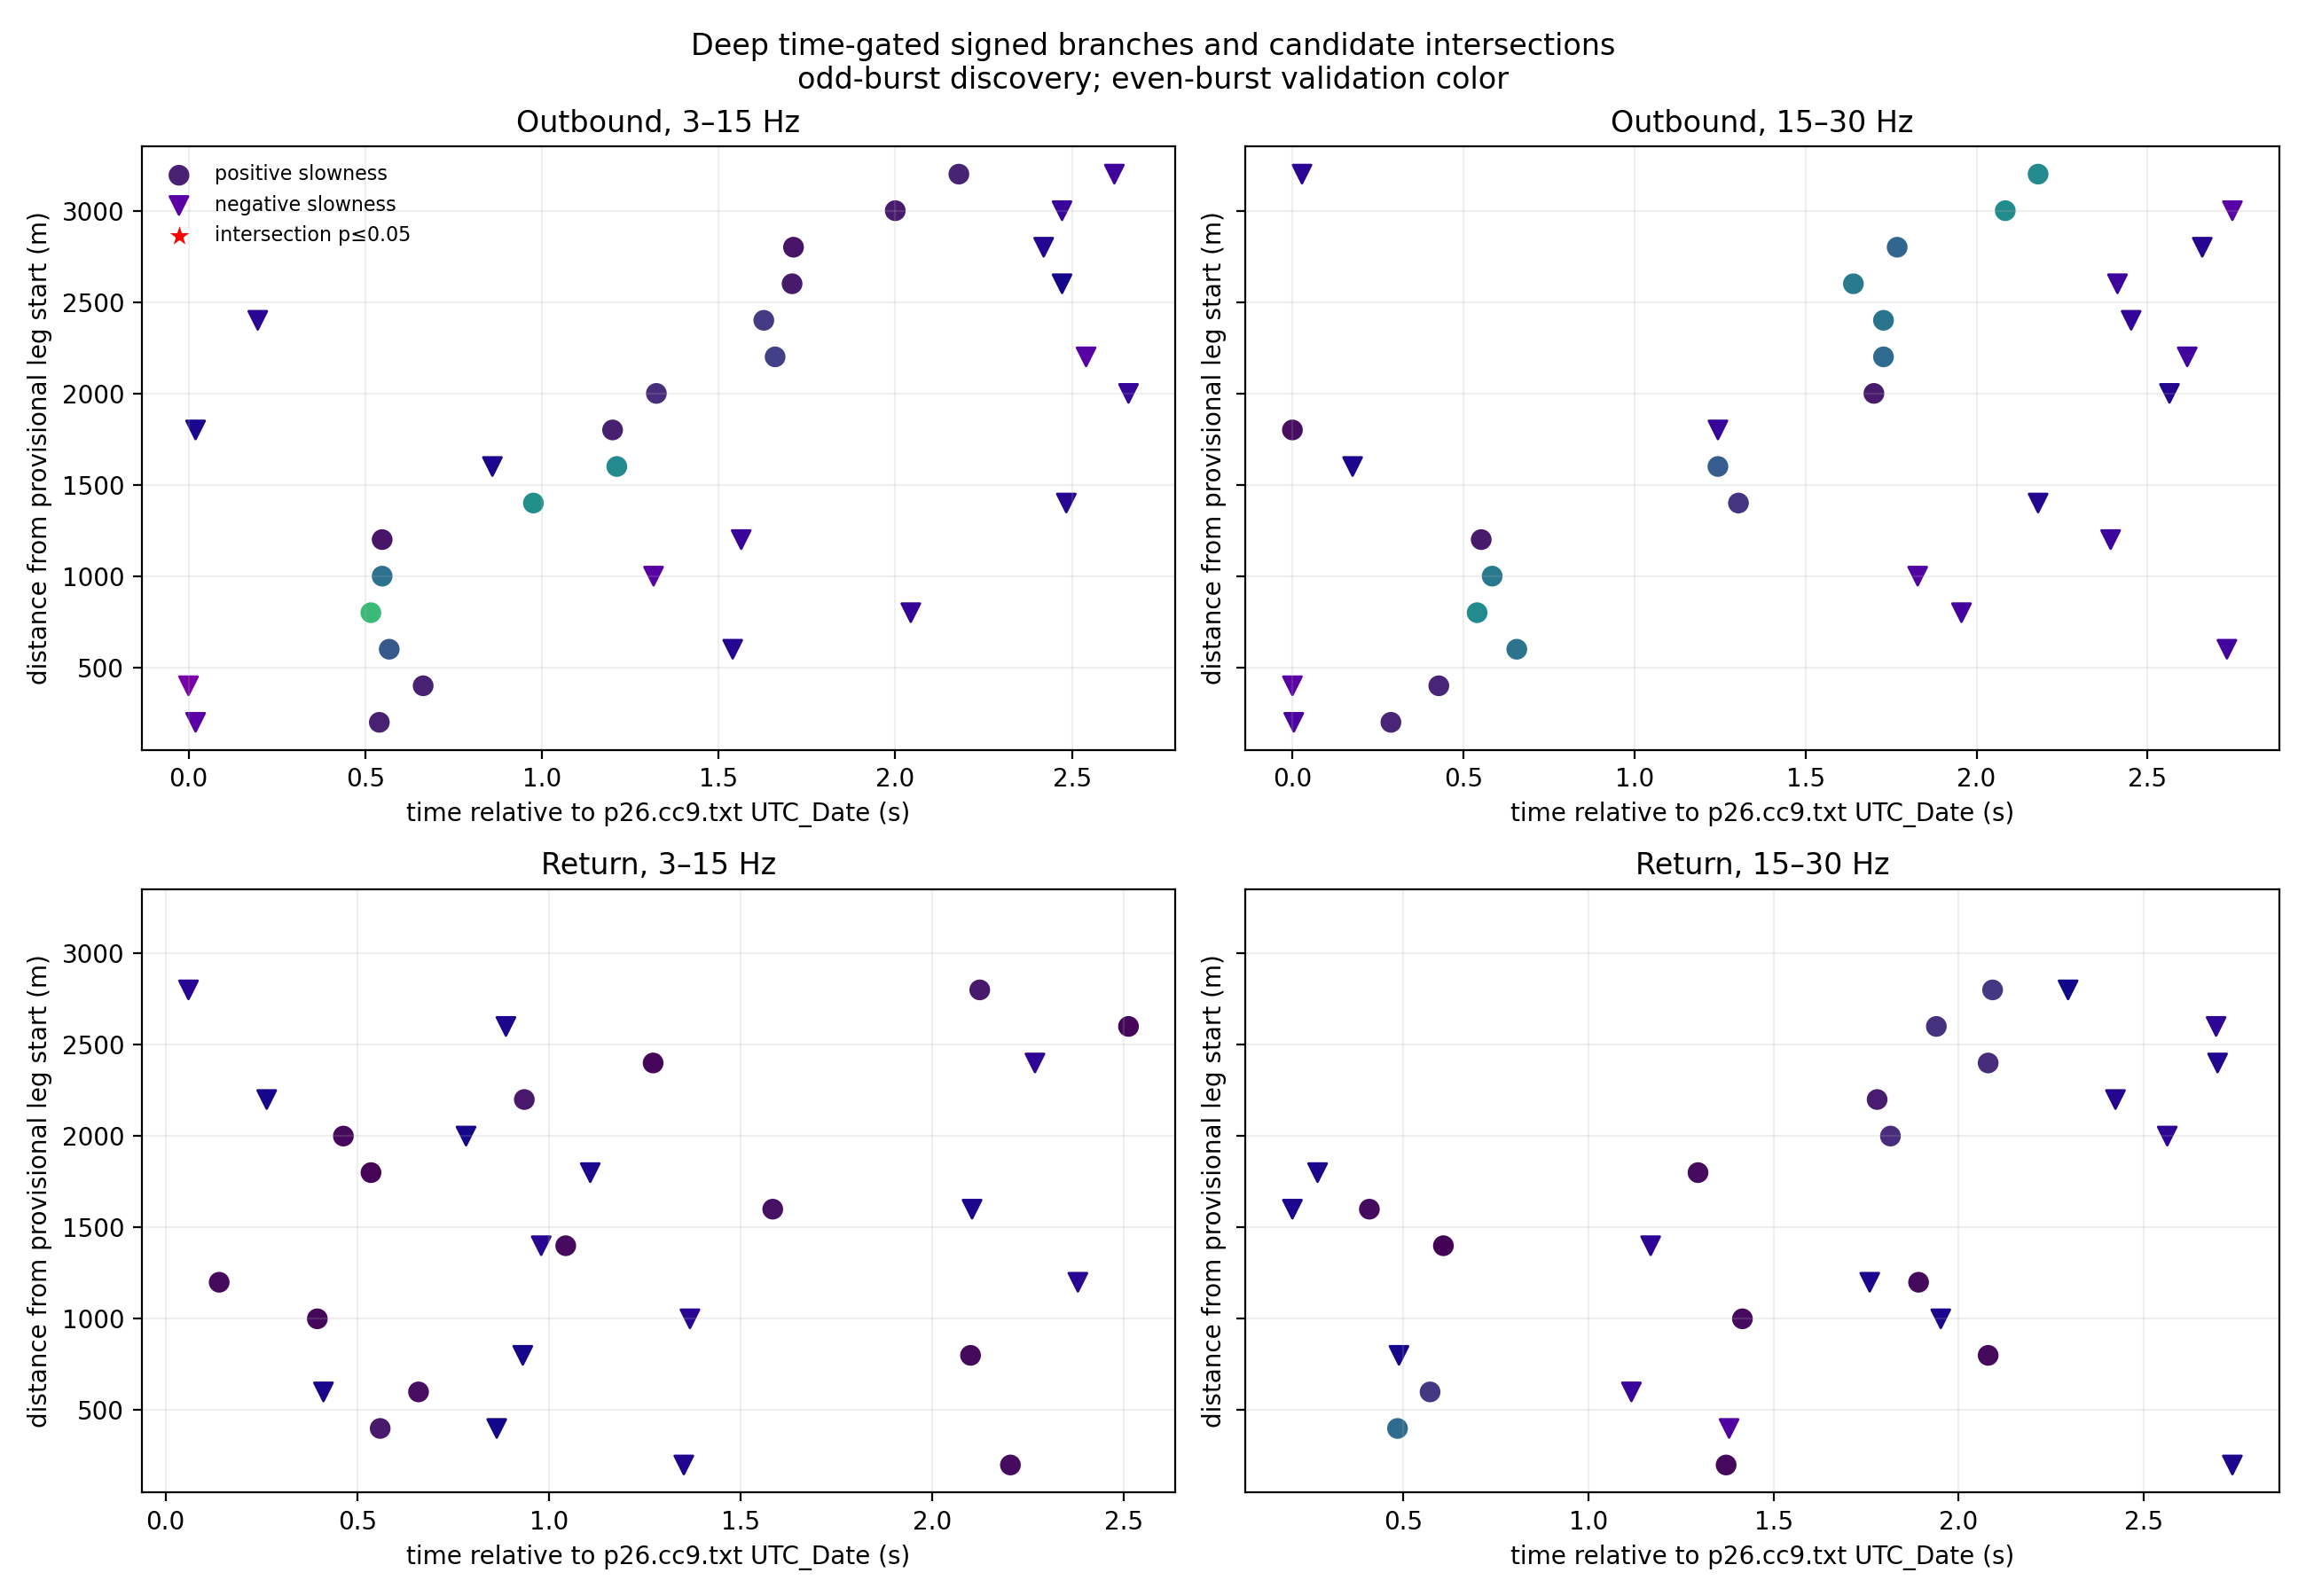
\includegraphics[width=0.91\linewidth]{deep_time_gated_branches.png}
\caption{\textbf{Time-gated signed Deep branches and candidate intersections.}
Rows show outbound and reversed-return legs; columns show 3--15 and 15--30~Hz.
Circles and inverted triangles are positive- and negative-slowness candidates
found in 400~m apertures.  Horizontal position is candidate time relative to
\code{p26.cc9.txt UTC\_Date}; vertical position is distance from the provisional
leg start.  Odd bursts select the gate and trajectory, while marker color gives
even-burst validation semblance.  Red stars would mark a positive/negative
geometric intersection with joint permutation $p\leq0.05$.  Among 120 tested
branch rows, five geometric intersections occur, but none passes the joint
permutation threshold.  Thus the present data and estimator do not support a
defensible fixed conversion or reflection coordinate.  All positions remain
fiber coordinates, not true depth or accepted fracture locations.}
\end{figure}

\takeaway{Accepted negative result: the slow Deep mode is real, but this test
does not validate a conversion/reflection depth.  A permeability or fracture
claim would therefore be premature.}

\subsection{Supplemental diagnostic: What apparent-velocity change can the present Nano method detect?}
\figquestion{Given real inter-burst noise and waveform variability, what is the
smallest imposed change in the accepted Nano moveout observable that is
recovered with high reliability?}

The reference trajectory is fixed at $2.975~\mathrm{km\,s^{-1}}$ in the
30--60~Hz, 80--440~m Nano aperture.  Known positive, negative, and zero changes
are injected into real burst observations.  Recovery is blind with respect to
the injection label.  The null median is removed as an empirical calibration;
the remaining zero-injection distribution measures false alarms.

\begin{figure}[H]
\centering
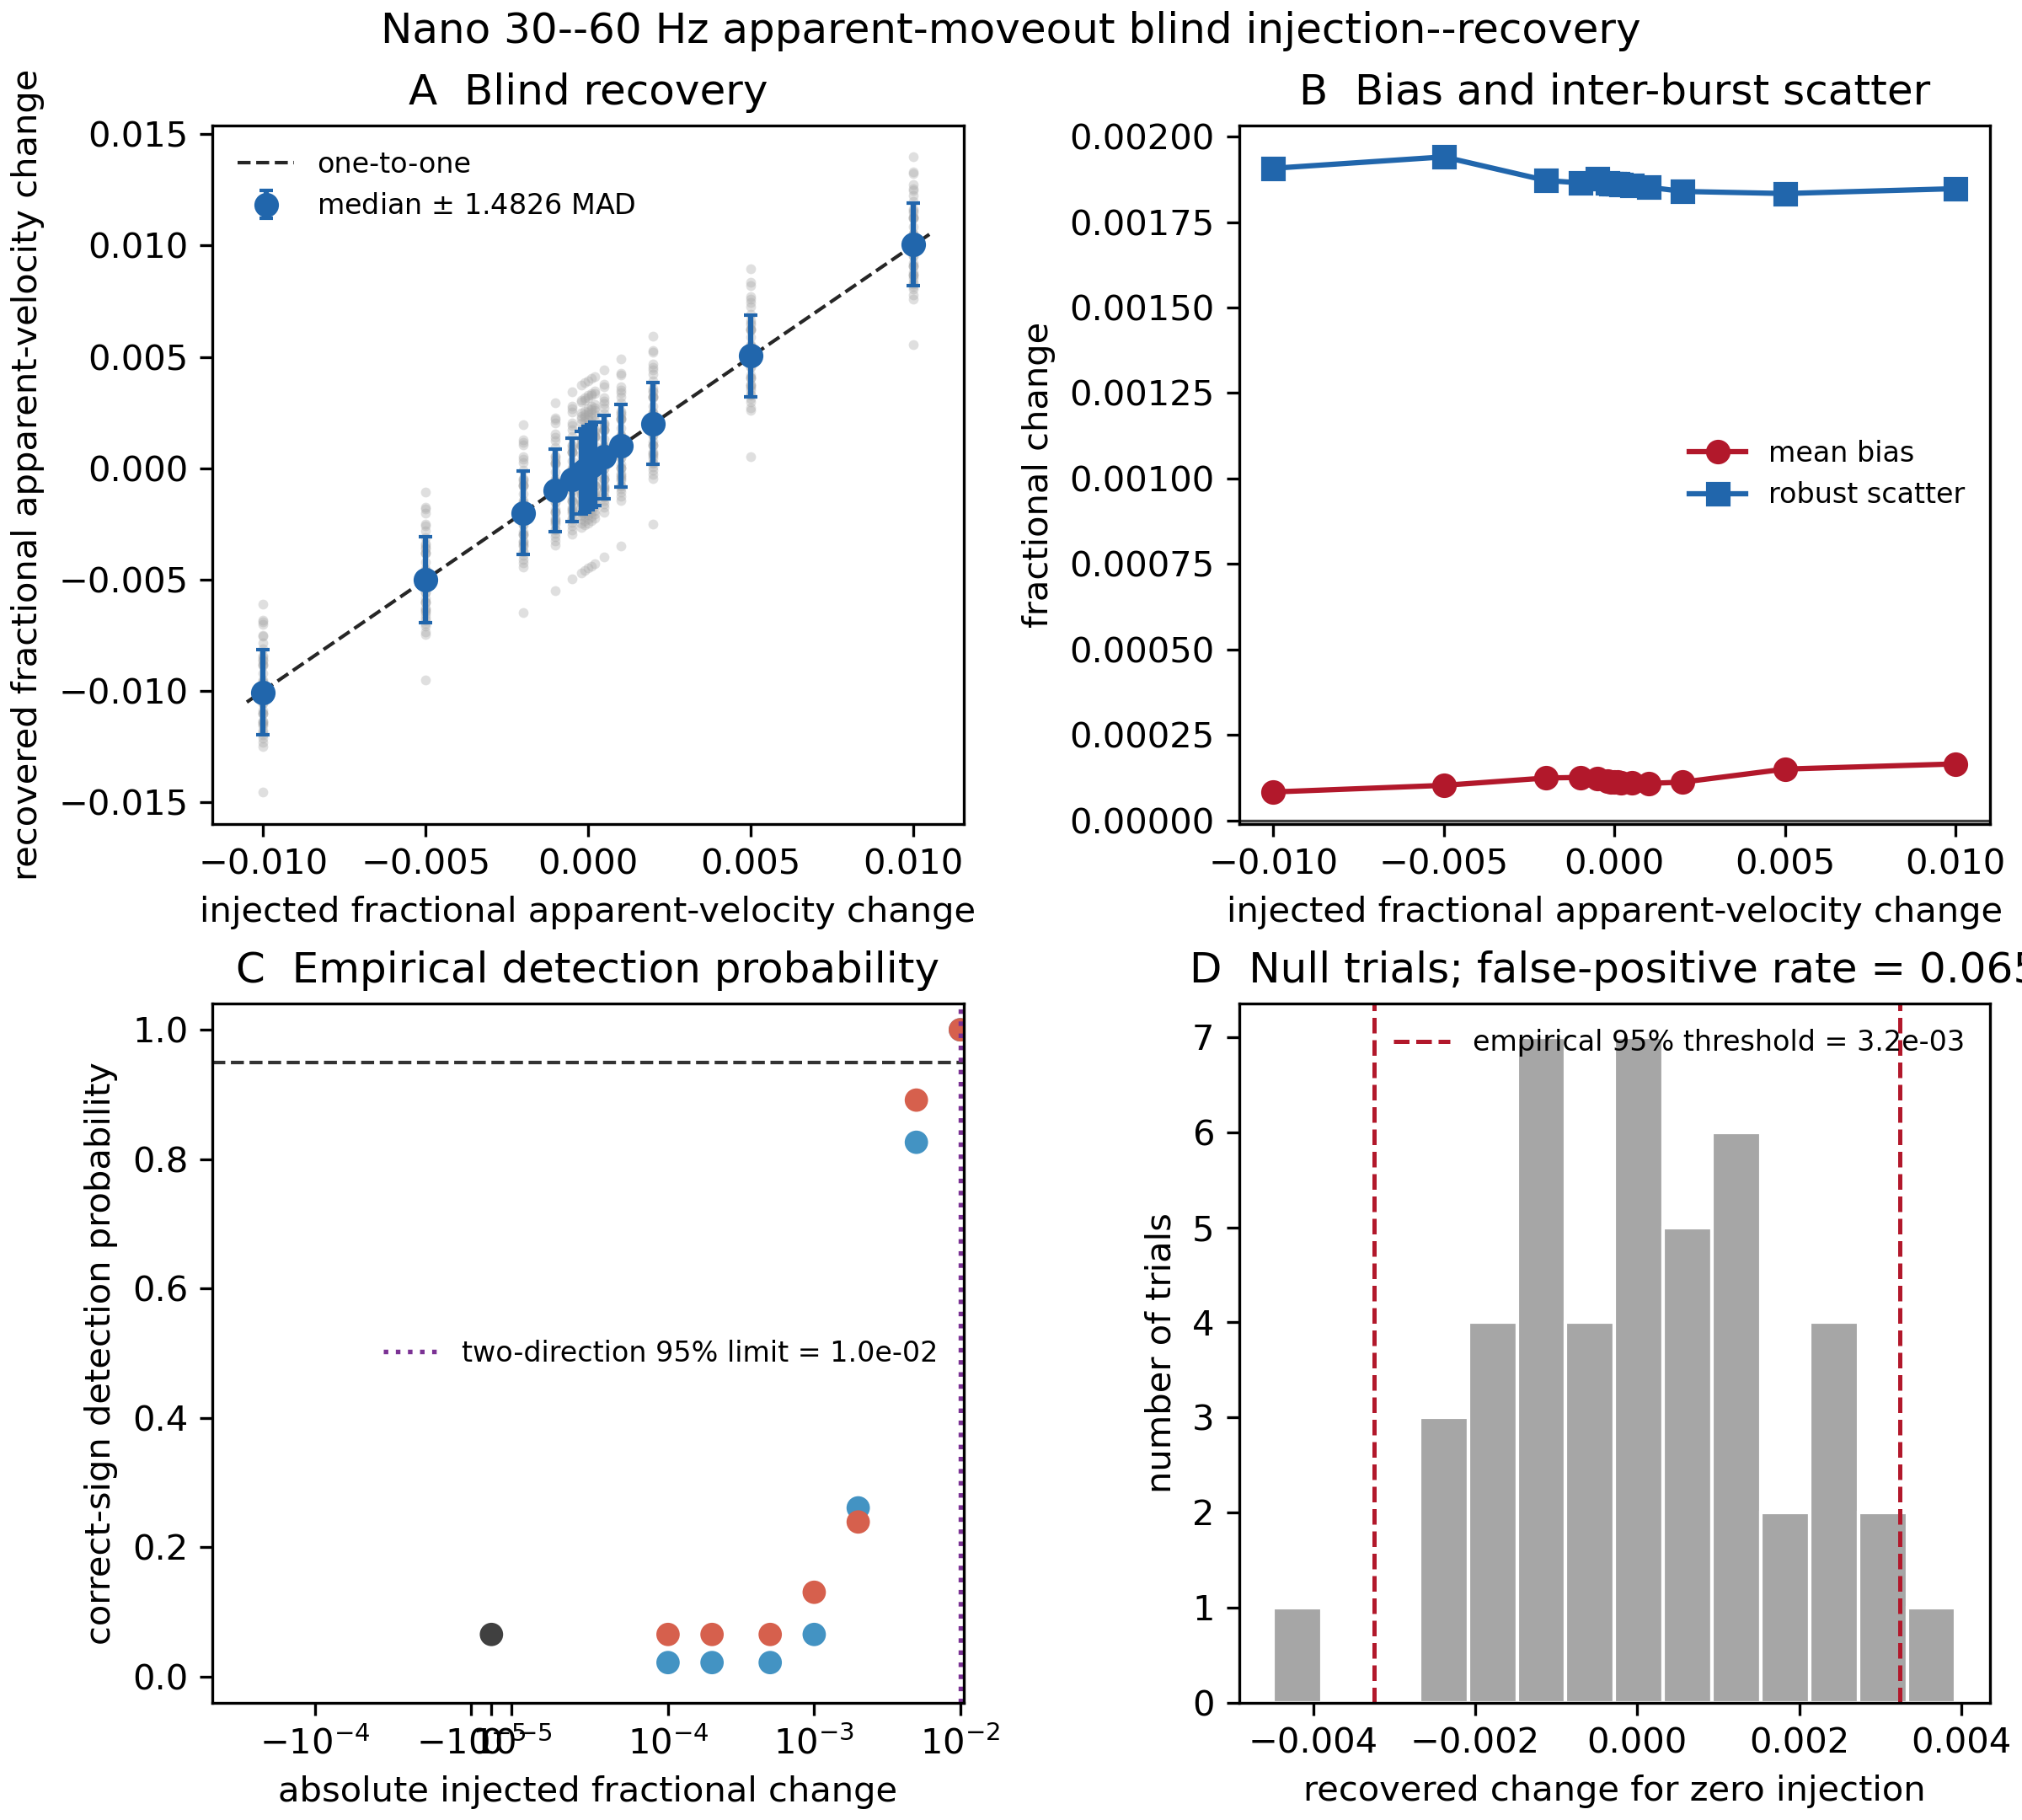
\includegraphics[width=0.82\linewidth]{nano_dvv_injection_recovery.png}
\caption{\textbf{Blind injection--recovery for the Nano 30--60~Hz
apparent-moveout observable.} (a) Recovered versus injected fractional
apparent-velocity change for 690 trials; blue summaries show the median and
1.4826 times the median absolute deviation, and the dashed line is ideal
one-to-one recovery.  (b) Mean recovery bias and robust inter-burst scatter as
functions of injected change.  (c) Empirical probability of recovering the
correct sign; the 95\% target must be achieved for both positive and negative
injections of a given magnitude.  The smallest tested magnitude satisfying
that rule is $|\Delta v_{\rm app}/v_{\rm app}|=0.01$.  (d) Recovered values for
46 zero-injection trials after subtracting the null median; dashed lines mark
the empirical two-sided 95\% threshold of 0.00325.  The observed false-positive
rate is 0.065, close to but slightly above the nominal 0.05 level because only
46 null trials are available.  This is a detection limit for fractional change
in the chosen apparent-moveout estimator under the current burst-level design.
It is not yet a direct-P formation $\Delta V_P/V_P$ limit, and Earth-tide-scale
changes have not been detected.}
\end{figure}

\takeaway{Current empirical result: 1\% is the smallest tested magnitude with
at least 95\% correct-sign recovery in both directions.  The null width is much
larger than typical Earth-tide-scale velocity changes, so the present estimator
does not yet justify an Earth-tide sensitivity claim.}

\section{Additional results}

The authoritative dashboard was promoted to v18 after the corrected hierarchical
repeatability rerun, the Deep split-sample and time-gated branch search, the
SAFOD-model forward and stack-sensitivity branches, the all-shot PGSI
timing/moveout calibration, the Deep coordinate-registration/forward test, the
source-history/tidal-timescale regression, exploratory and physically phased CCA controls, and the six-figure core presentation set were
synchronized.  These products are loaded
directly by the notebook and should be discussed together rather than as
independent claims.

\subsection{Figure 12: Individual-drop and burst repeatability}
\figquestion{Is the selected Nano moveout observable stable within individual
AWD bursts and across the full experiment?}

The analysis uses 988 extracted drops from 49 bursts.  Each drop is aligned only
to the fixed 30--60~Hz, 80--440~m apparent-moveout trajectory.  Signal NCC is
computed in the selected moveout window and compared with an equal-duration
pre-signal noise window.  Leave-one-burst-out templates test across-burst
stability, while independent within-burst substacks show convergence with
repetition.

\begin{figure}[H]
\centering
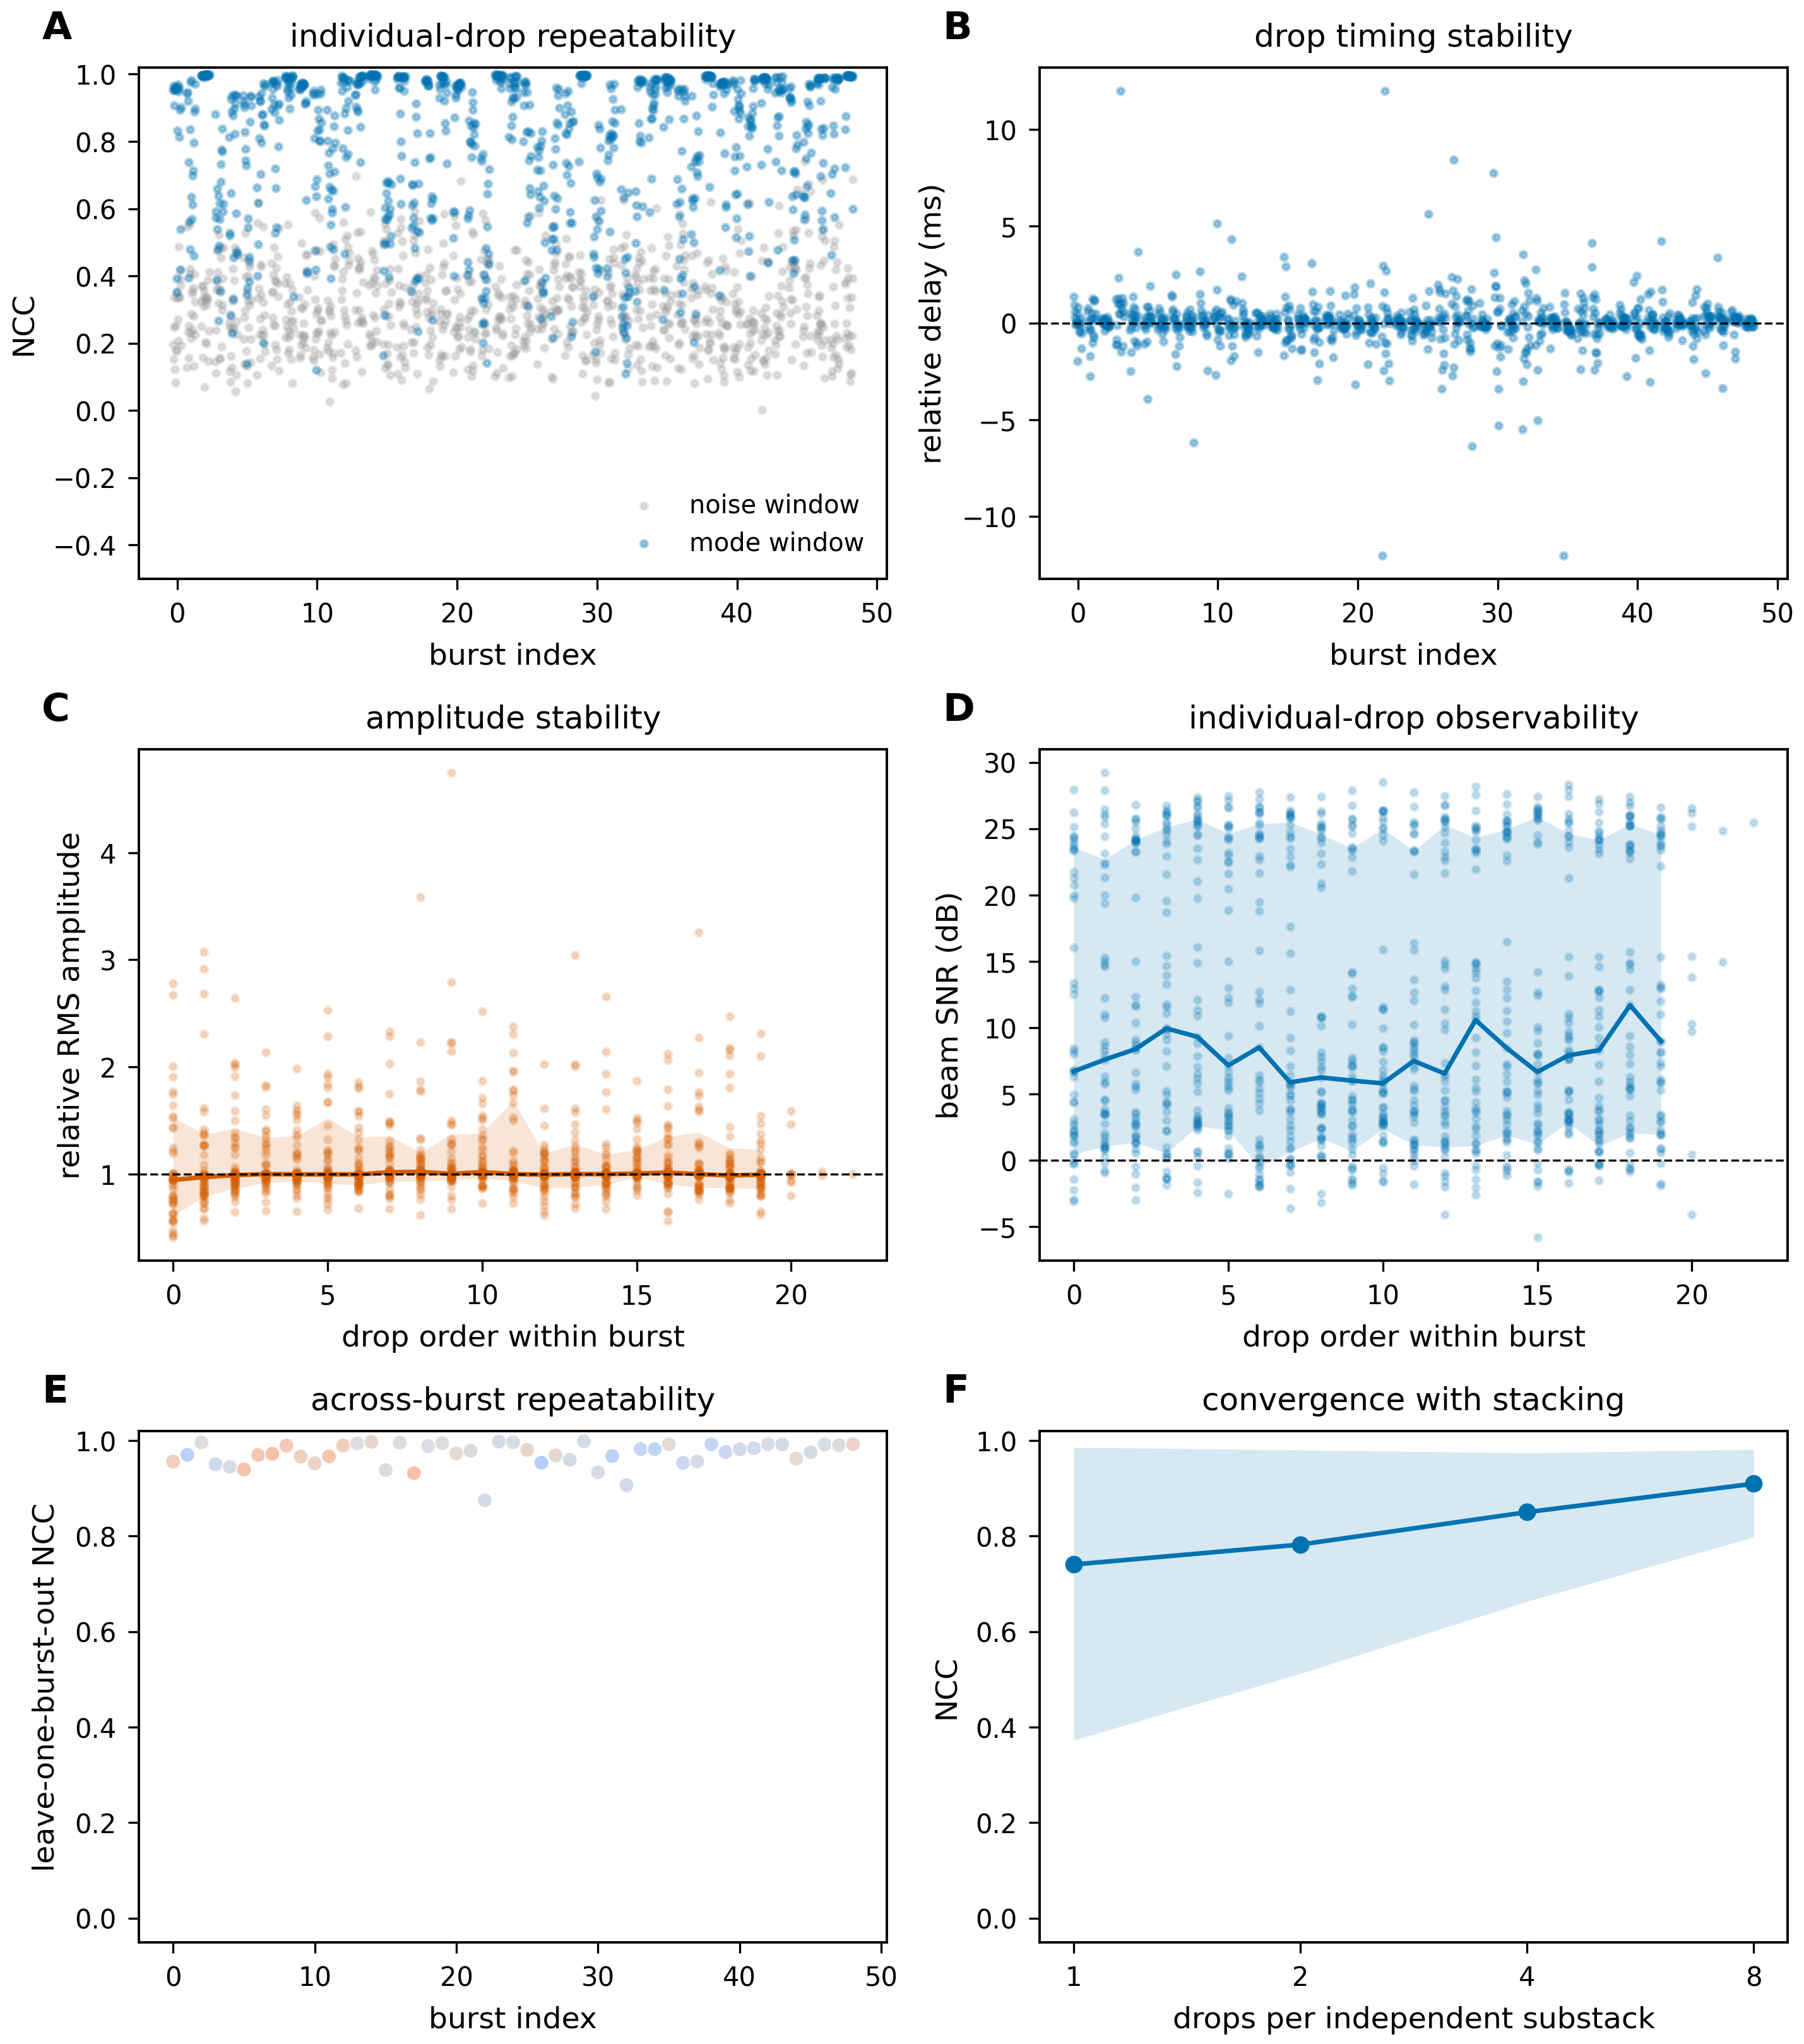
\includegraphics[width=0.95\linewidth]{fig12_repeatability_publication.png}
\caption{\textbf{Hierarchical repeatability of the Nano AWD moveout observable.}
Each drop contributes one signal and one equal-duration noise NCC measurement;
summary bars report the 16th, 50th, and 84th percentiles.  All 49 bursts have a
larger median signal NCC than noise NCC (exact one-sided sign-test
$p=1.78\times10^{-15}$), with medians 0.889 and 0.288, respectively.  The
leave-one-burst-out template comparison has median NCC 0.976 and median delay
$-0.048$~ms.  Independent-substack curves are plotted only where at least ten
bursts contribute, preventing late drop orders represented by a few unusually
long bursts from being overinterpreted.  Delays and amplitudes are relative
observables because catalog alignment is not an absolute impact-time
calibration.  The figure establishes repeatability of a phase-neutral
moveout beam; it does not identify direct P, constrain formation $V_P$, or
calibrate absolute source radiation.}
\end{figure}

\takeaway{\accepted repeatability result: the Nano observable is reproducible
within bursts and across bursts, providing the statistical basis for monitoring
sensitivity experiments.}

\subsection{Figure 13: SAFOD-model forward identifiability test}
\figquestion{Does the transferred SAFOD 3-D velocity prior automatically predict
the observed approximately 3~km~s$^{-1}$ Nano ridge as direct P?}

The Zhang--Thurber--Bedrosian grid is parsed from
\code{Vp\_model.dat}, \code{Vs\_model.dat}, \code{Vpvs\_model.dat},
\code{MOD.head}, and \code{inversion\_grid.dat}.  Slowness is integrated along
representative shallow straight paths, and synthetic DAS moveout sections are
made for a direct-P model and a deliberately low-parameter weakly dispersive
guided alternative.

\begin{figure}[H]
\centering
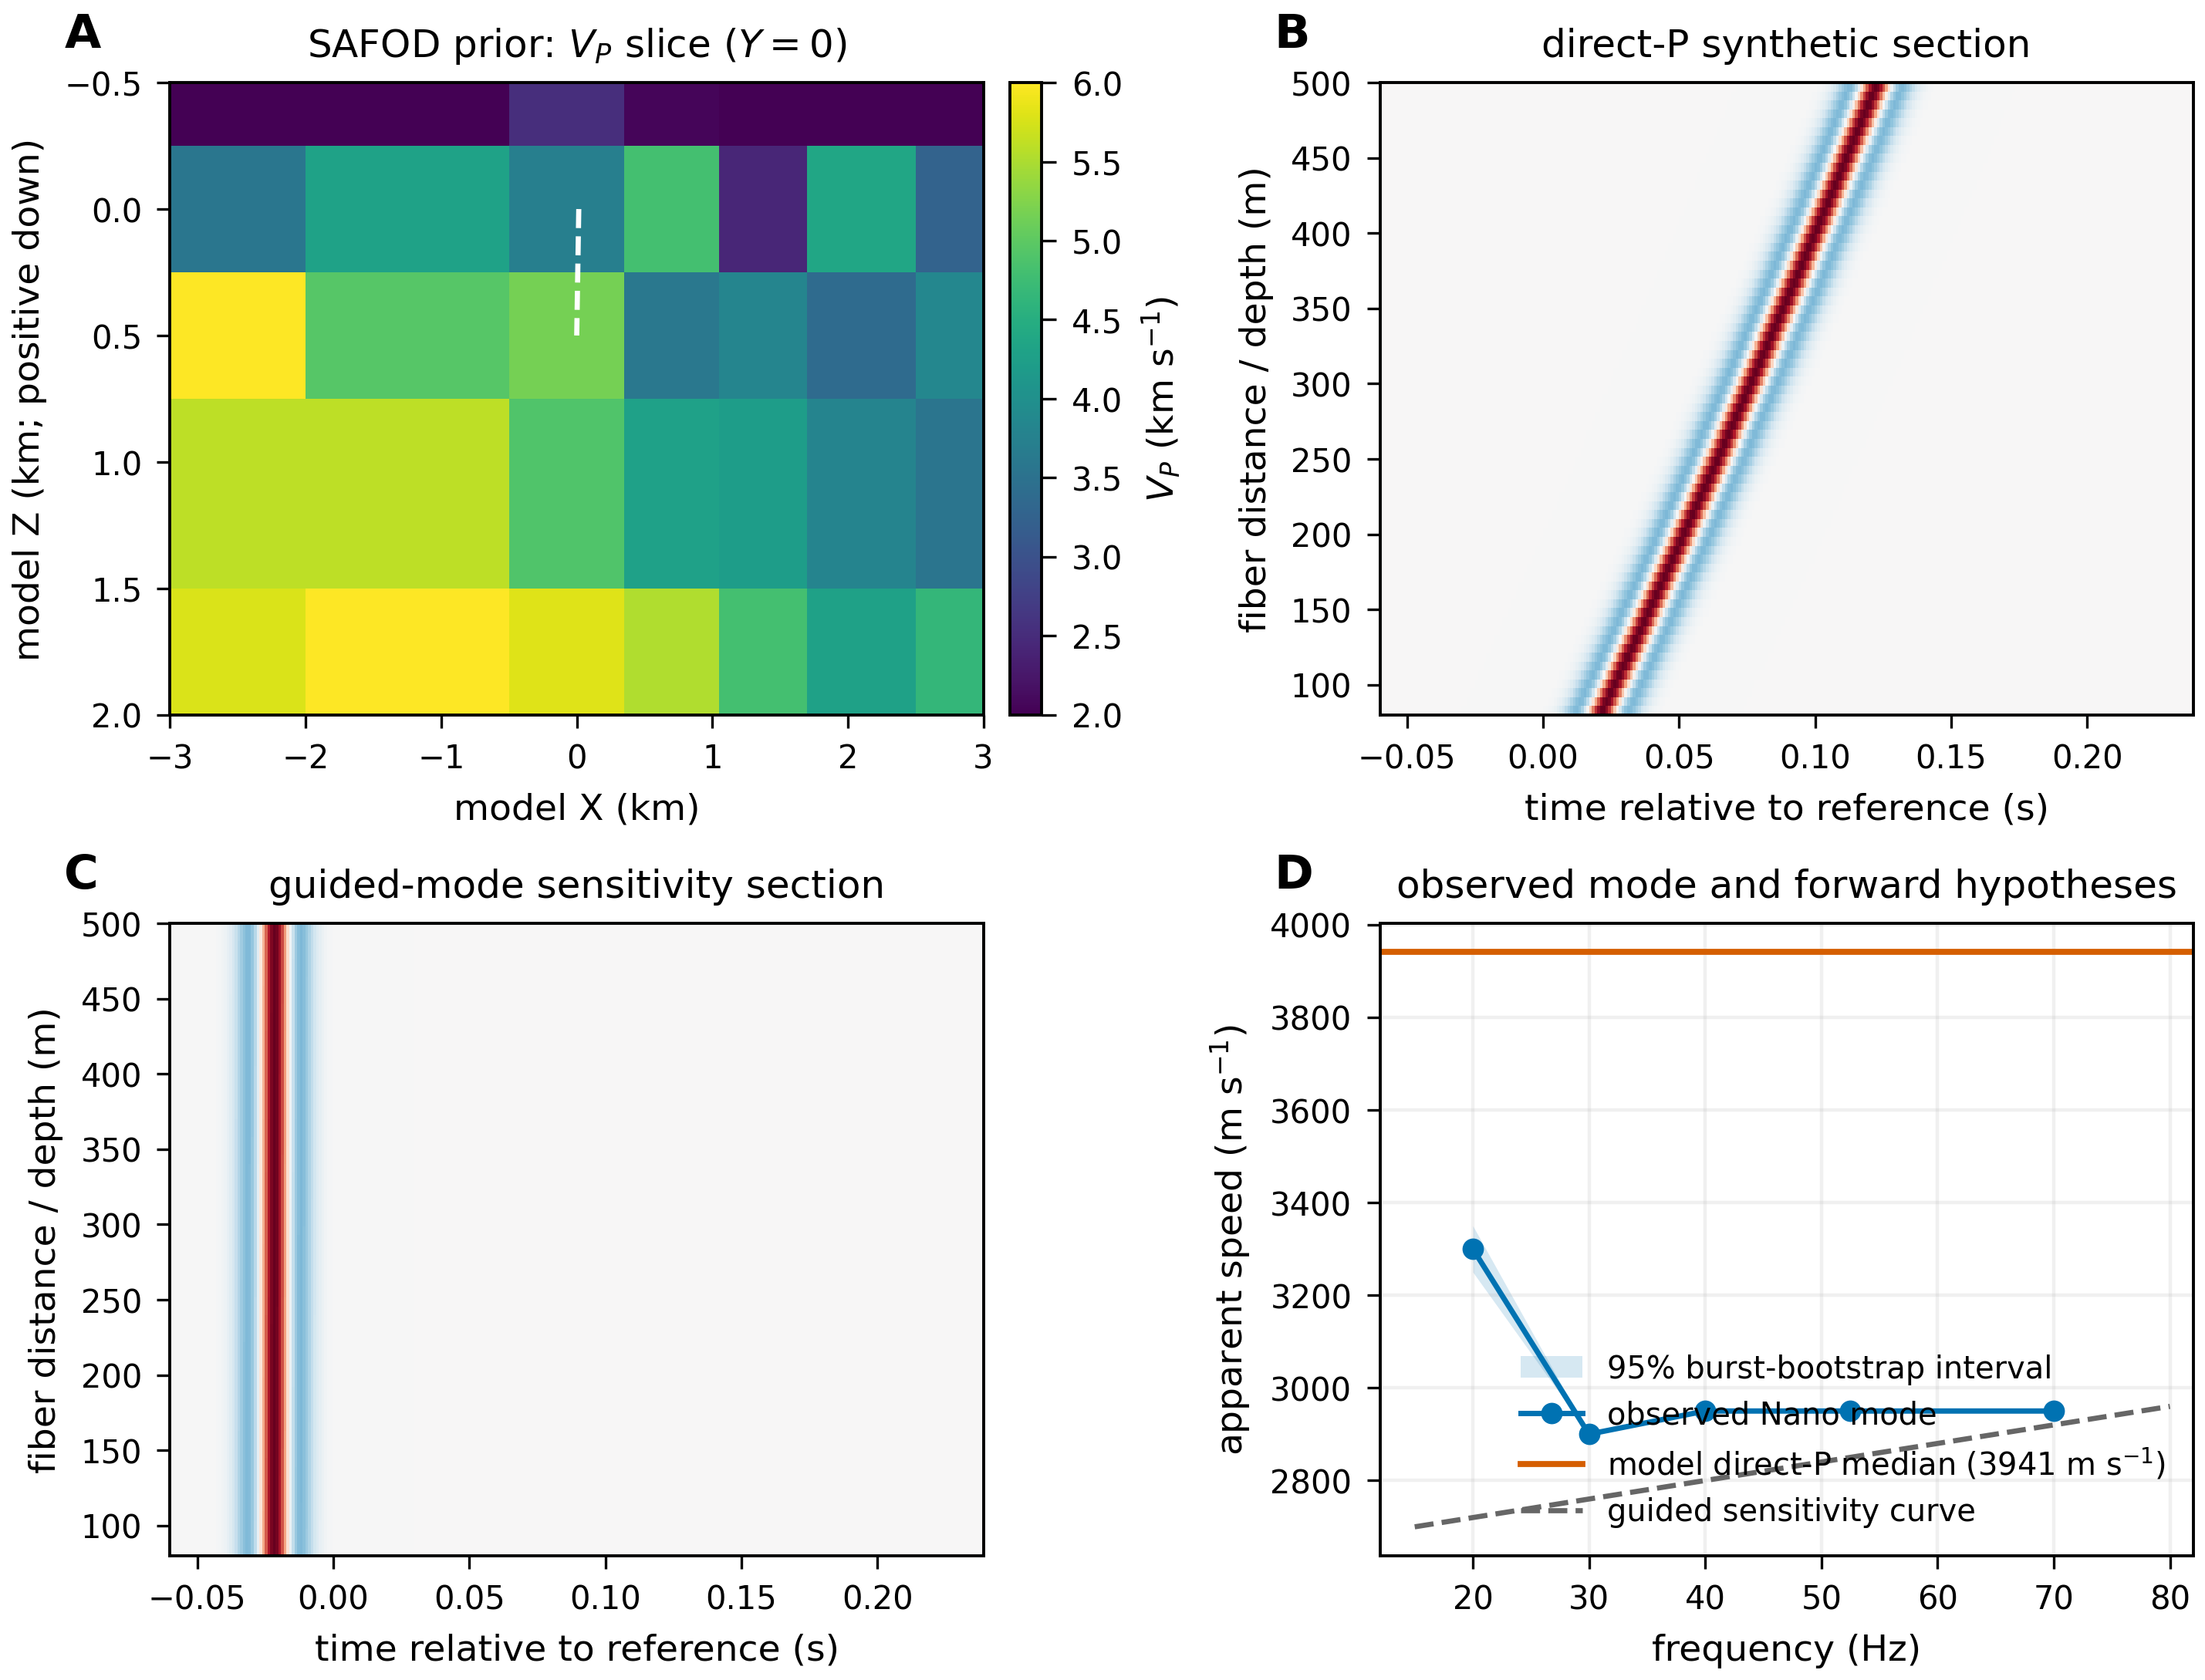
\includegraphics[width=0.95\linewidth]{fig13_forward_publication.png}
\caption{\textbf{Forward comparison using the SAFOD velocity prior.} (A) A
vertical slice of the transferred $V_P$ prior in model coordinates. (B) A
synthetic direct-P section formed by integrating $1/V_P$ from a representative
source to 80--500~m offsets. (C) A weakly dispersive guided sensitivity curve,
$c(f)=2.72+0.004(f-20)$~km~s$^{-1}$, is shown as a hypothesis anchored near
the observed ridge rather than as an asserted tube-wave law. (D) Observed Nano
apparent speeds and bootstrap intervals are compared with the forward curves.
The corrected vertical-fiber path has median speed approximately 3.94~km~s$^{-1}$,
above the observed 2.95--2.99~km~s$^{-1}$ ridge.  This mismatch motivates
geometry-, anisotropy-, and path-aware modeling; it is not by itself evidence
against direct P and is not a $V_P$ inversion.}
\end{figure}

\takeaway{\preliminary sensitivity result: the geological prior does not make
the observed apparent speed automatically equal to formation $V_P$; phase
identification and geometry calibration remain necessary.}

\subsection{Figure 14: Stack-size monitoring sensitivity}
\figquestion{How does repeated stacking change the smallest apparent-moveout
perturbation that can be detected?}

The measured zero-injection distribution supplies a baseline null standard
deviation of 0.00175.  A transparent $1/\sqrt{N}$ independence model projects
thresholds for $N=1,2,4,8,16,32,46$ independent stacks; empirical NCC
convergence is shown separately.  The $5\times10^{-4}$ line is an illustrative
Earth-tide-scale comparison target, not a detected signal.

\begin{figure}[H]
\centering
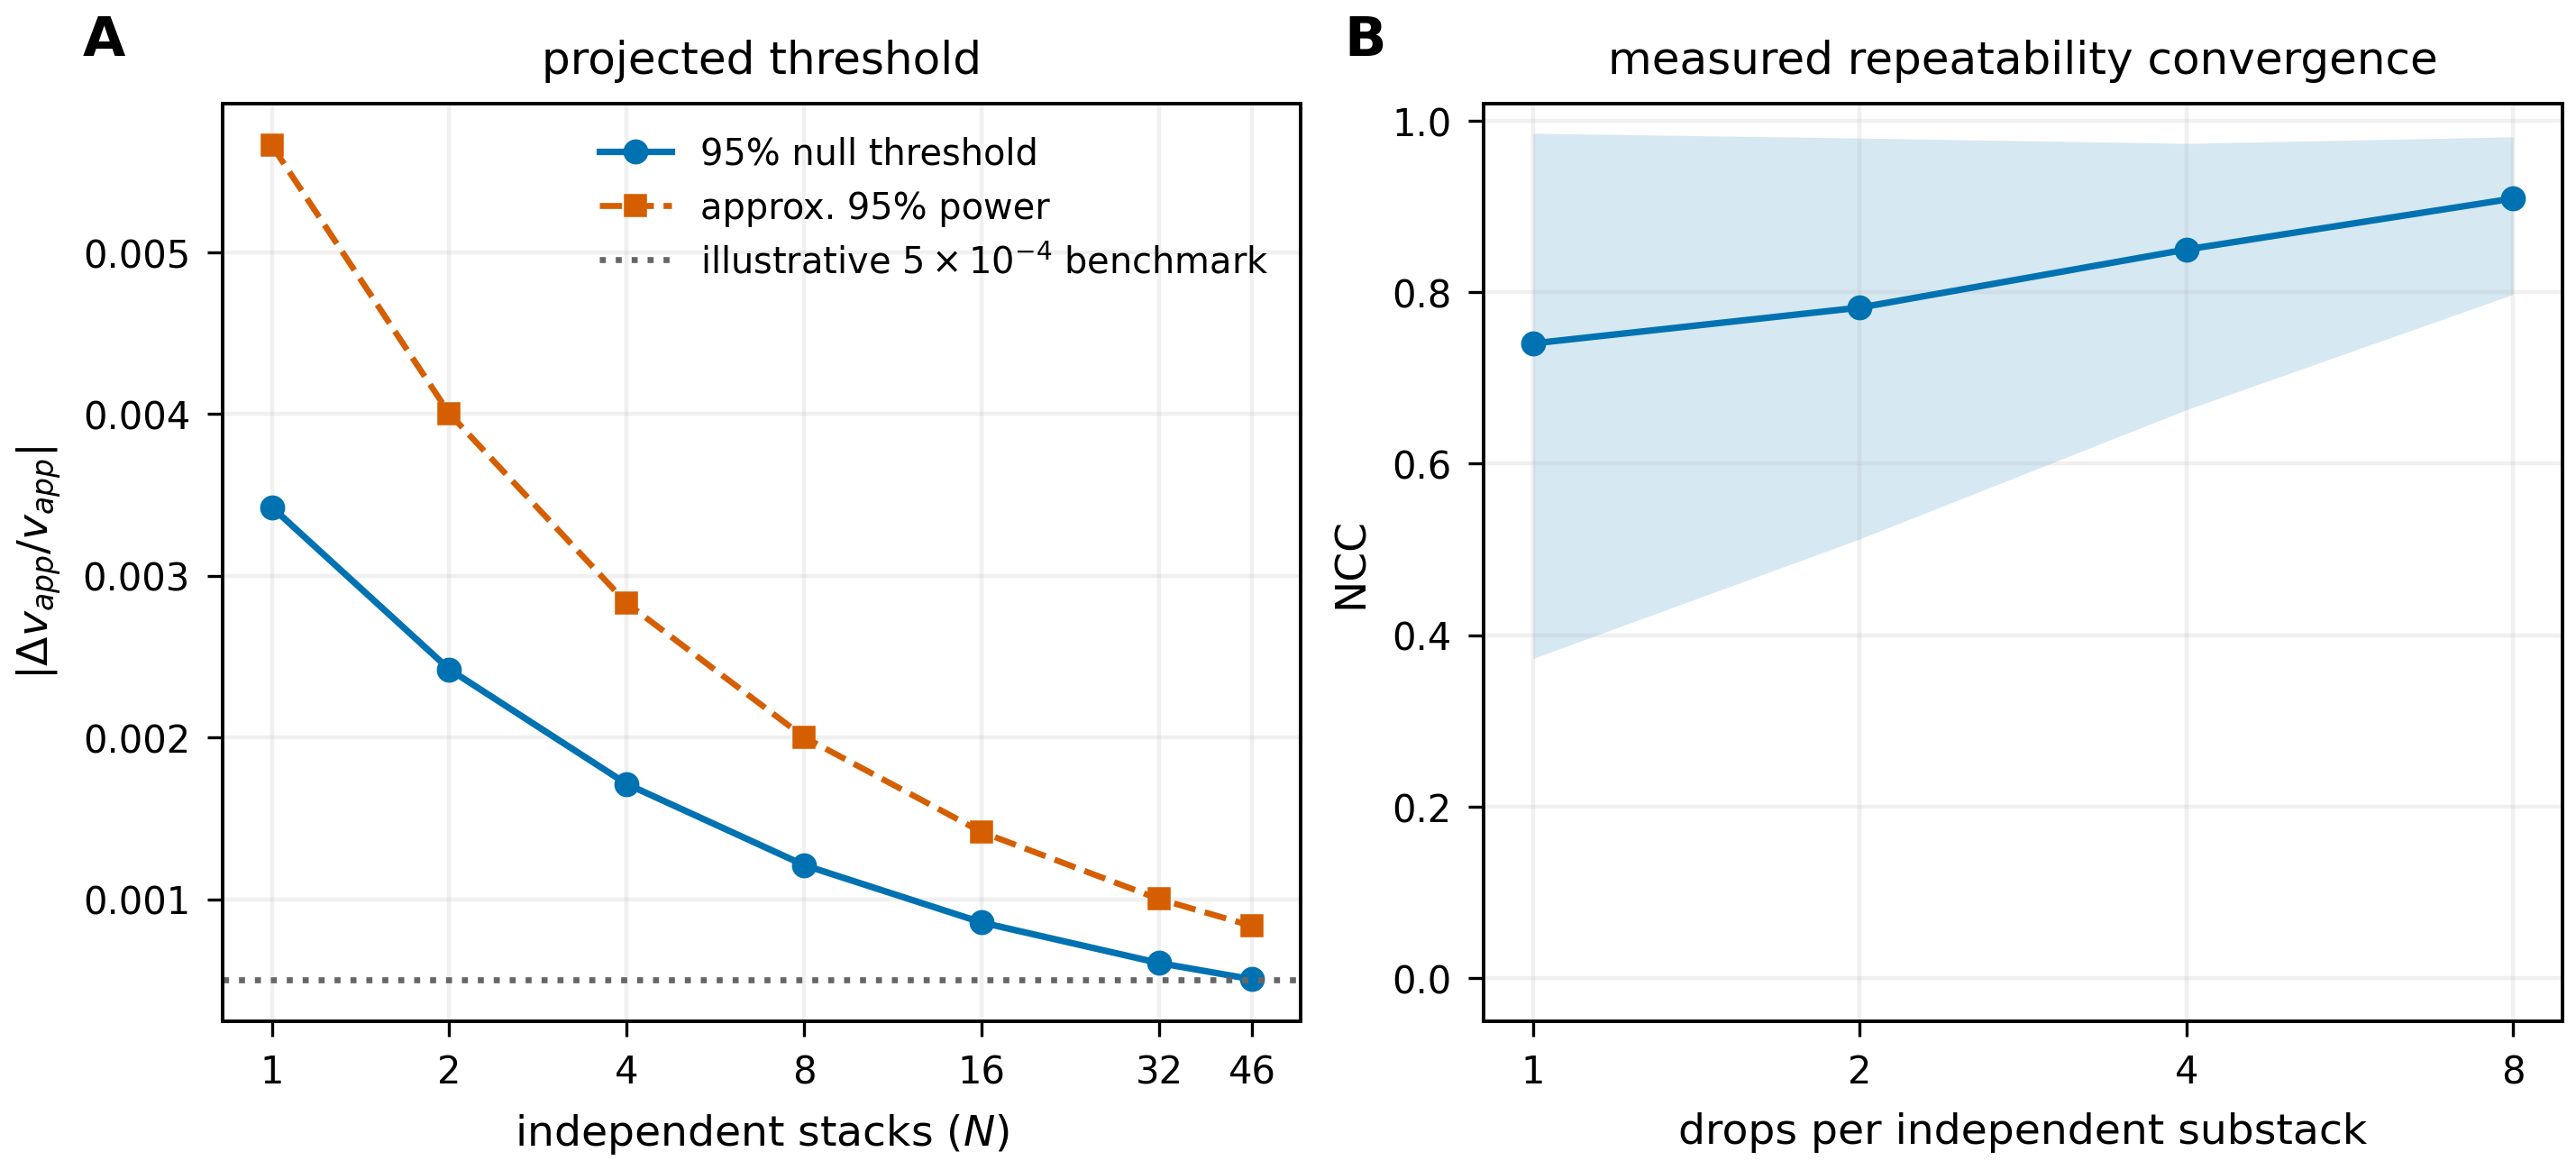
\includegraphics[width=0.95\linewidth]{fig14_monitoring_publication.png}
\caption{\textbf{Stack-size dependence of monitoring sensitivity.} (A) Solid
and dashed curves are the projected two-sided 95\% null and approximate 95\%
power thresholds after $1/\sqrt{N}$ scaling of the measured null width.  The
dotted line is an illustrative $5\times10^{-4}$ benchmark.  (B) Points and
central 68\% intervals are empirical NCC values for independent within-burst
sub-stacks.  The left panel is a design projection that assumes independent
stacks; the right panel is measured repeatability.  Both apply only to the
accepted Nano apparent-moveout observable and must not be relabeled a direct
formation $\Delta V_P/V_P$ threshold or a demonstrated tidal response.}
\end{figure}

\takeaway{\accepted at observable level: injection--recovery and repeatability
now provide a defensible monitoring-sensitivity result, while Earth-tide-scale
resolution remains below the present one-day experiment's demonstrated limit.}


\subsection{Figure 15: PGSI all-shot timing reconciliation and moveout fits}
\figquestion{Can one explicit timing convention be applied to all six PGSI
records, which shots provide defensible moveout fits, and does the registered
moveout agree with the Nano depth-axis slope?}

This is the immediate calibration decision because the Nano mode is statistically
secure but physically underidentified as direct formation P versus guided or
coupled energy.  The PGSI records are controlled explosions rather than AWD
drops and use three-component geophones rather than 2026 DAS.  They provide the
independent surveyed receiver depths, source offsets, channel ordering, and
legacy timing note needed to test a geometry-corrected moveout before discussing
a formation $V_P$.  Position 1 spans 46.677--1249.777~m measured depth, and the
maximum measured-depth versus vertical-depth discrepancy is 0.864~m.

The catalog explosion times in \texttt{shot\_locs.doc} define the physical
origins.  SEG2 \code{ACQUISITION\_TIME} is file-start metadata, not the
explosion time.  The supplied R note states that file zero is 200~ms before
shot origin; consequently every record is fit on the common axis
$t=i/200-0.200~s$.  Header \code{DELAY} values are retained as QC rather
than silently rewriting the records.  The six bookkeeping cases are: 1027
(36.000386~s acquisition-to-catalog, header $-0.200$~s), 1040
(36.000197~s, $-0.200$~s), 1060 (36.000124~s, $-0.200$~s), 1071
(1.000018~s, header $+0.200$~s), 1078 (1.000043~s, $-0.200$~s), and 1082
(35.000000~s, header 0.000~s).  Thus 1071 and 1082 retain explicit +0.400-s
and +0.200-s header-versus-canonical differences; no absolute impact trigger
is claimed.

The script \path{pgsi_checkshot_allshots.py} maps axial channels 3, 6,
..., 240 and reverses their deep-to-shallow file order.  A robust AIC onset
picker is fit against source--receiver slant distance with fixed 30-ms residual
rejection and bootstrap confidence intervals.  A record is usable only when
at least 20/80 receiver picks survive, RMS is at most 20~ms, and speed is
between 1.5 and 8~km~s$^{-1}$.  These are transparent calibration criteria,
not a geological phase classifier.

Five of six records pass.  Shot 1027 is rejected (8/80 picks).  The retained
fits are 1040: $2.982~[2.923,3.032]~$km~s$^{-1}$, 38/80 picks, 3.09-ms RMS;
1060: $5.451~[5.333,5.555]~$km~s$^{-1}$, 68/80, 6.33~ms; 1071:
$5.472~[4.924,6.301]~$km~s$^{-1}$, 20/80, 14.76~ms (marginal); 1078:
$5.198~[5.056,5.358]~$km~s$^{-1}$, 63/80, 8.13~ms; and 1082:
$5.411~[5.306,5.564]~$km~s$^{-1}$, 73/80, 5.35~ms.  Shot 1040 is the
only usable fit whose interval overlaps the Nano apparent-speed interval
2.95--2.99~km~s$^{-1}$.  The faster fits must not be averaged with it into a
single $V_P$.

\begin{figure}[H]
\centering
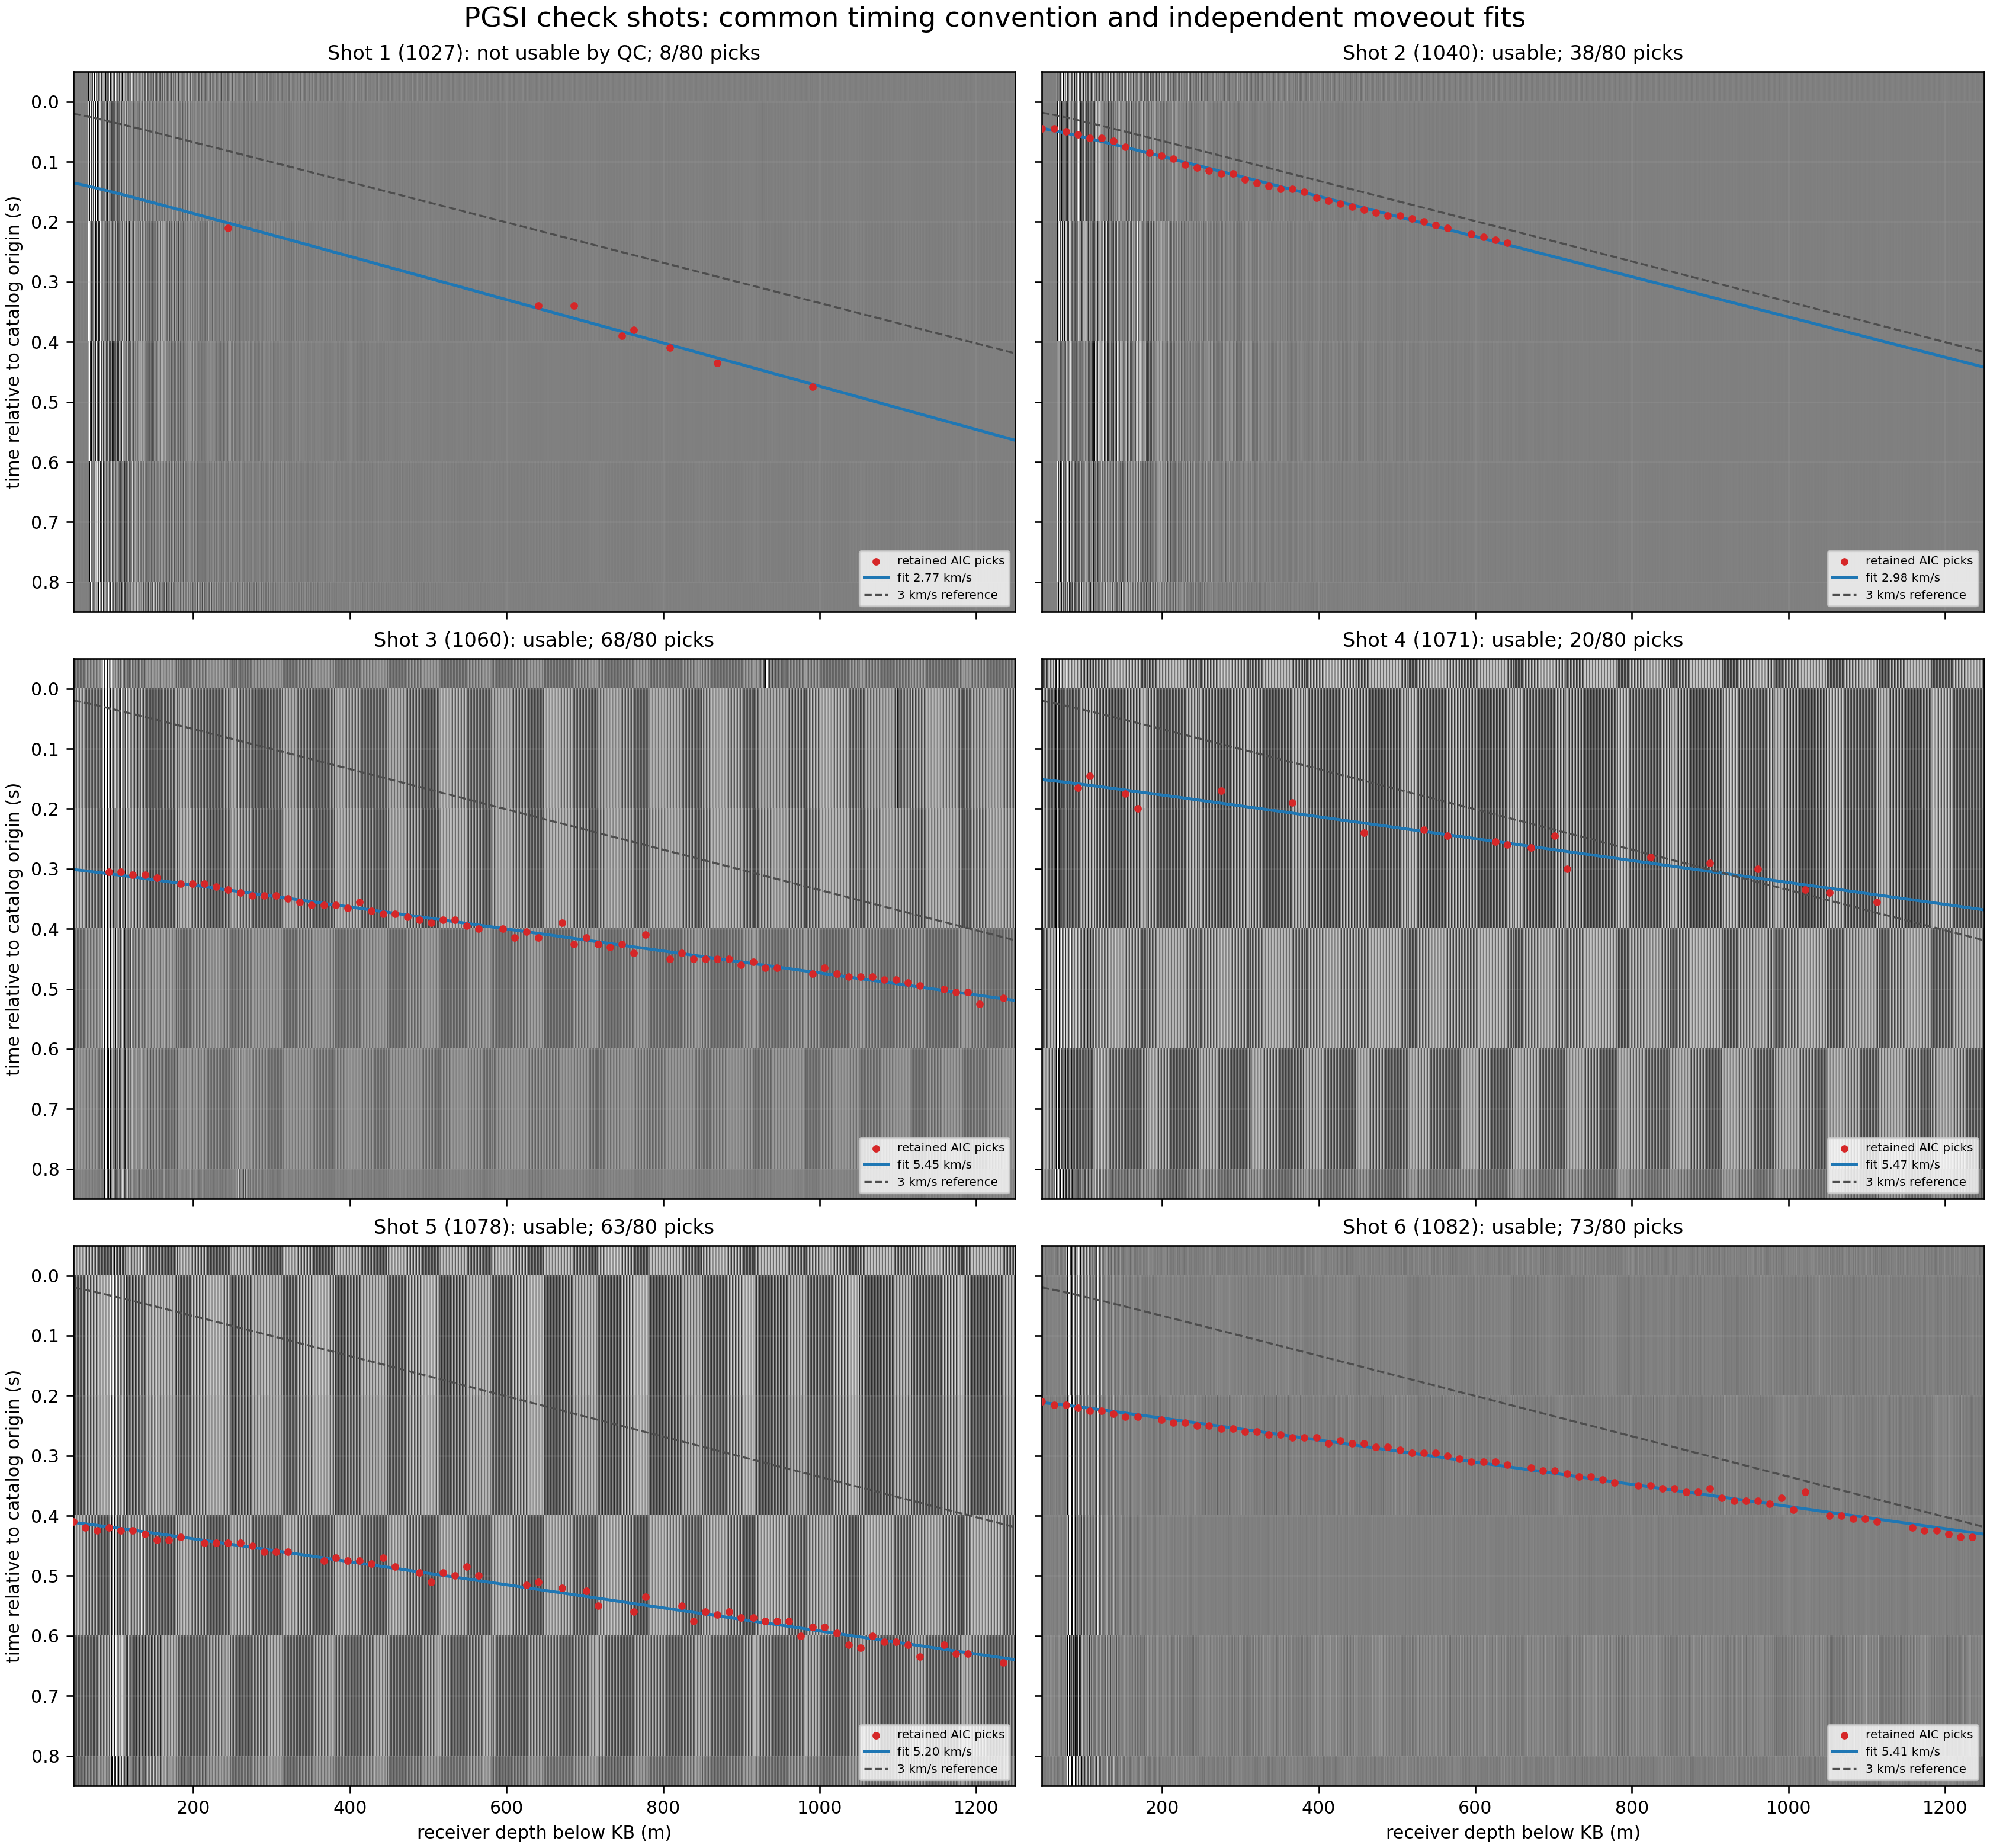
\includegraphics[width=0.98\linewidth]{../figures/awd_2026/pgsi_checkshot_allshots.png}
\caption{\textbf{PGSI all-shot timing reconciliation and geometry-corrected moveout fits.} The six panels show position-1 axial-component record sections for SEG2 files 1027, 1040, 1060, 1071, 1078, and 1082 on the common $t=i/200-0.200$~s axis, using channels 3, 6, ..., 240 reversed to shallow--deep order. Traces are independently normalized only for display; colored curves are robust slant-distance fits and red points are AIC onsets retained by the fixed 30-ms residual criterion. Panel annotations report retained picks, speed, 95\% bootstrap interval, fitted origin, and RMS. Shot 1027 fails QC with 8/80 picks. Shot 1040 is the only fit in the Nano 2.95--2.99~km~s$^{-1}$ interval: $2.982~[2.923,3.032]$~km~s$^{-1}$, 38/80 picks, and 3.09-ms RMS. Shots 1060, 1071, 1078, and 1082 are faster (5.20--5.47~km~s$^{-1}$); 1071 is marginal because only 20/80 picks survive and its interval is broad. The figure identifies which records support reproducible moveout under one documented timing convention; it does not identify a P phase, recover an absolute impact-time correction, or provide a formation $V_P$ inversion.}\end{figure}

\subsection{Figure 16: Conditional registration with the Nano depth axis}
\figquestion{Does the PGSI moveout register with the Nano depth axis under the least-assumption slope test?}

The registration removes each PGSI fitted origin offset and compares relative
travel-time slopes.  Nano coordinates 80--440~m are plotted against PGSI
measured depth only as a conditional hypothesis test; no absolute PGSI-to-Nano
time equality or channel-to-depth identity is assumed.  Shot 1040 is the only
usable fit entering the Nano 2.95--2.99~km~s$^{-1}$ band.  The other usable
shots remain faster and are shown rather than discarded, because their
separation is evidence against collapsing the six records into one velocity.

\begin{figure}[H]
\centering
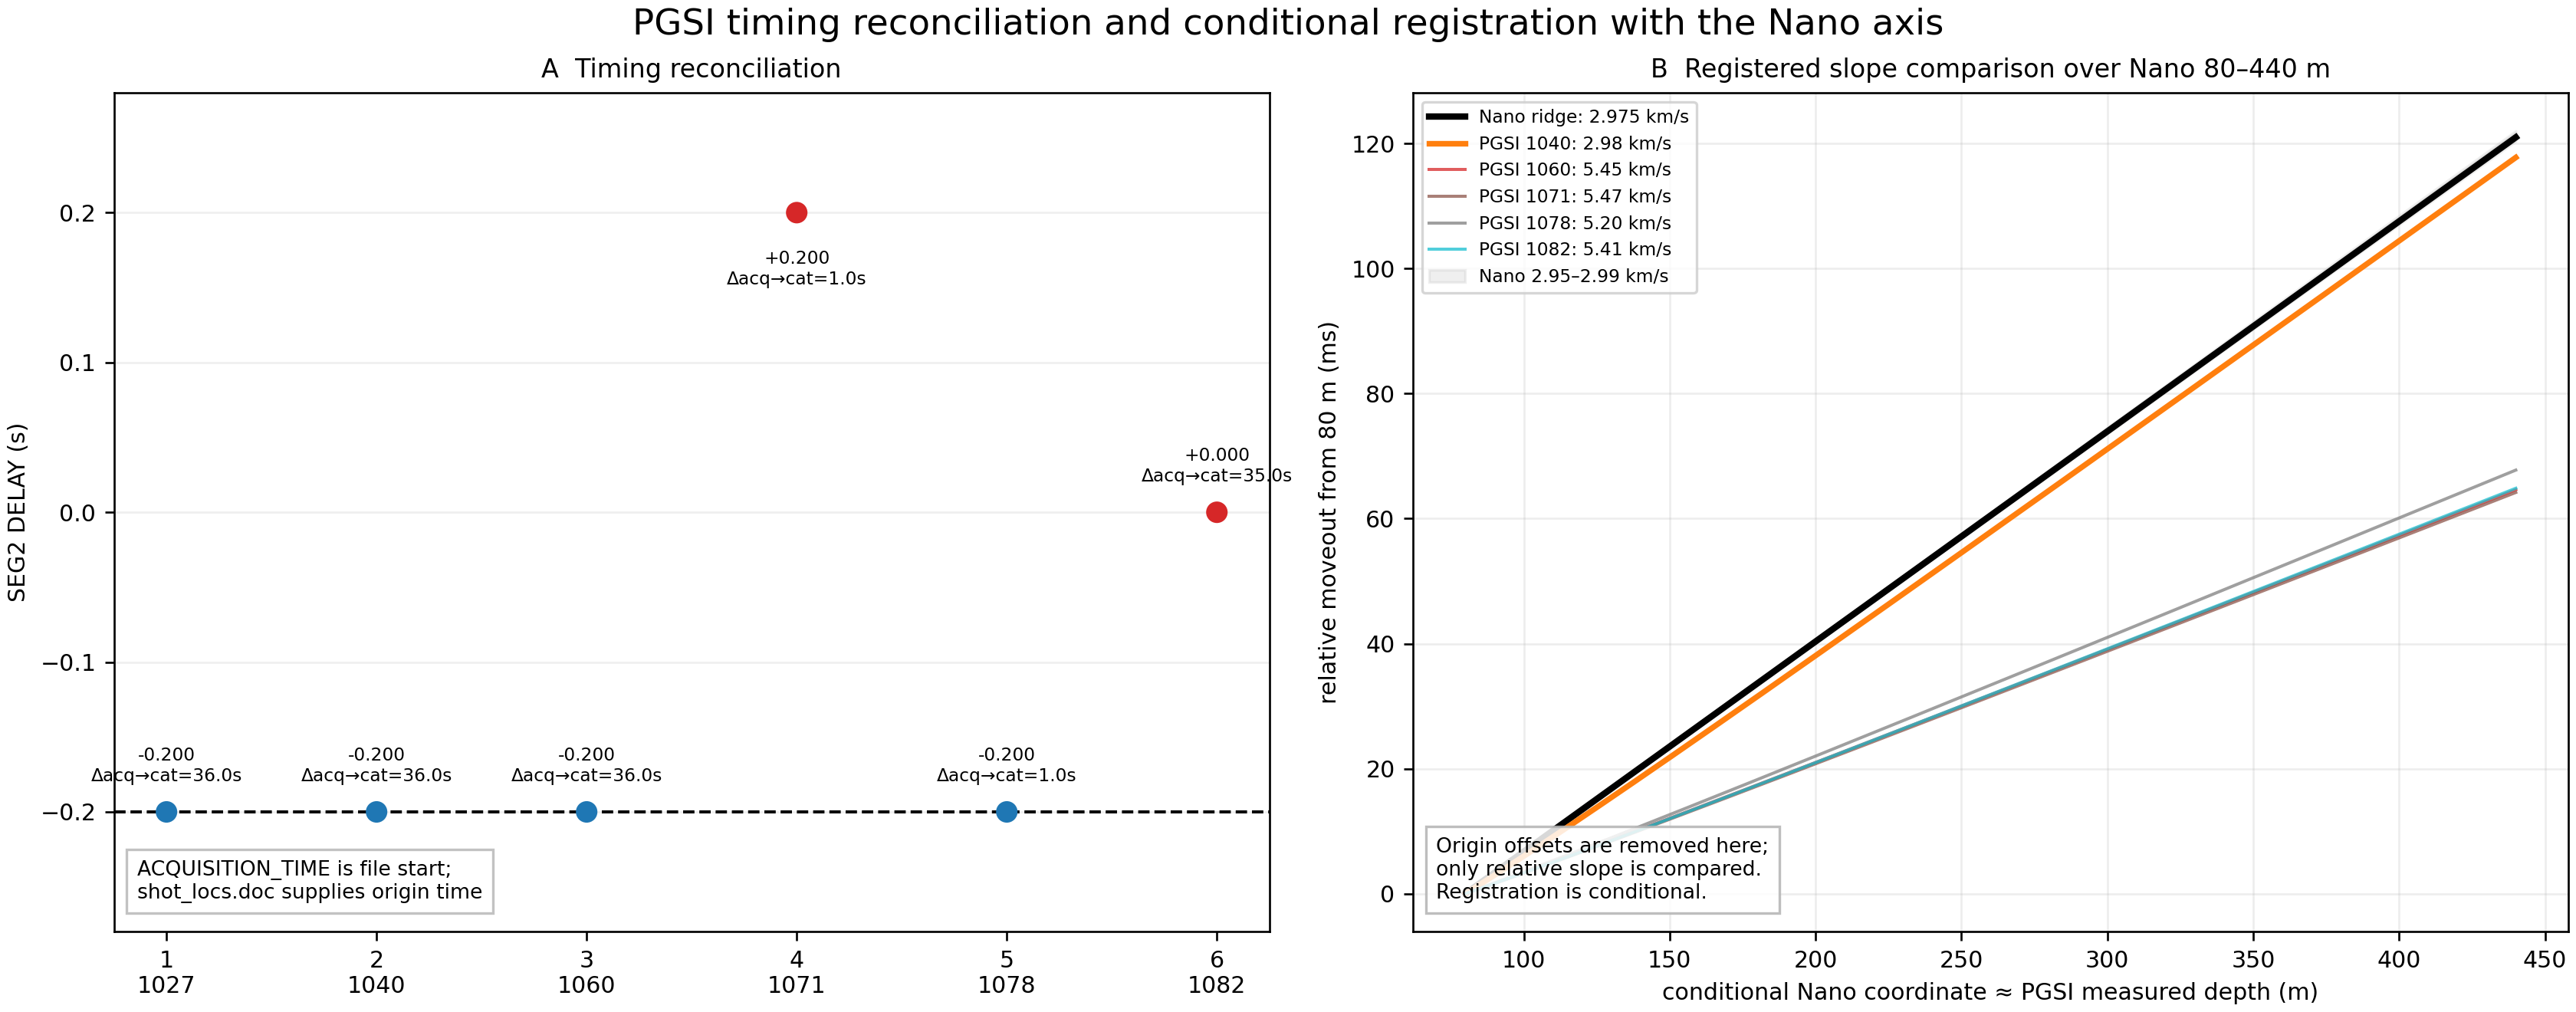
\includegraphics[width=0.98\linewidth]{../figures/awd_2026/pgsi_checkshot_registration.png}
\caption{\textbf{Conditional PGSI-to-Nano registration.} (a) Header \code{DELAY} values are compared with the common $-0.200$-s origin; acquisition-to-catalog intervals are shown separately because \code{ACQUISITION\_TIME} identifies file start while \texttt{shot\_locs.doc} supplies explosion origin. (b) After fitted origin offsets are removed, relative travel time is plotted versus PGSI measured depth and the Nano 80--440~m coordinate is overlaid only for slope compatibility. The gray band is the Nano apparent-speed interval 2.95--2.99~km~s$^{-1}$; shot 1040 is the only usable PGSI fit entering it. The faster 1060, 1071, 1078, and 1082 fits are retained as a direct check that no single $V_P$ should be reported. This is a conditional registration, not an absolute depth map, because source and receiver systems differ and the origin offsets have been removed; no phase identity or $V_P(z)$ inversion is claimed.}\end{figure}

\takeaway{\preliminary calibration result: one explicit timing convention yields five usable PGSI moveout fits, but only shot 1040 is compatible with the Nano approximately 3~km~s$^{-1}$ interval.  The registration is therefore a phase/geometry constraint, not a formation-$V_P$ result.}

\section{Figure 17: What does the Deep coordinate actually register?}
\figquestion{Are the Deep start-locus and hairpin coordinates measured depth, and is the validated slow mode compatible with a bounded tube-wave speed range?}

This test is required before any Deep feature can be called a fracture or
conversion depth.  The raw HDF5 metadata provide the interrogator
\code{StartLocusIndex=1800}, a 2.0419-m spatial sampling interval, and 3200
loci.  The validated Deep analyses split at channel 1702 and reverse the return
leg for a common provisional orientation.  These facts establish a reproducible
coordinate system: 3675.42 m for the start-locus coordinate, 3475.31 m for the
hairpin coordinate measured from channel 0, and 6532.04 m for the last locus.
None is a surveyed measured depth.  The HDF5 metadata contain no surveyed fiber
origin, cable path, casing or fluid properties, or physical-depth transform.

The 24 candidates in \path{deep_tube_candidates.csv} are compared with a
bounded sensitivity envelope: a 1.3--1.8-km-s$^{-1}$ fluid prior multiplied by
an explicitly phenomenological 0.75--1.0 compliance factor.  This is not a
fitted tube-wave dispersion law.  All candidates fall within the direct fluid
prior (median 1.538 km s$^{-1}$; 5th--95th percentile 1.389--1.563 km s$^{-1}$),
so the result is consistent with tube-wave-like kinematics.  It cannot
identify the phase, fit compliance, locate a fracture, or establish
permeability.  The transferred \path{vel_model/} arrays are plotted only as
formation-background context; no borehole logs or fiber-to-depth registration
were found in the workspace.

\begin{figure}[H]
\centering
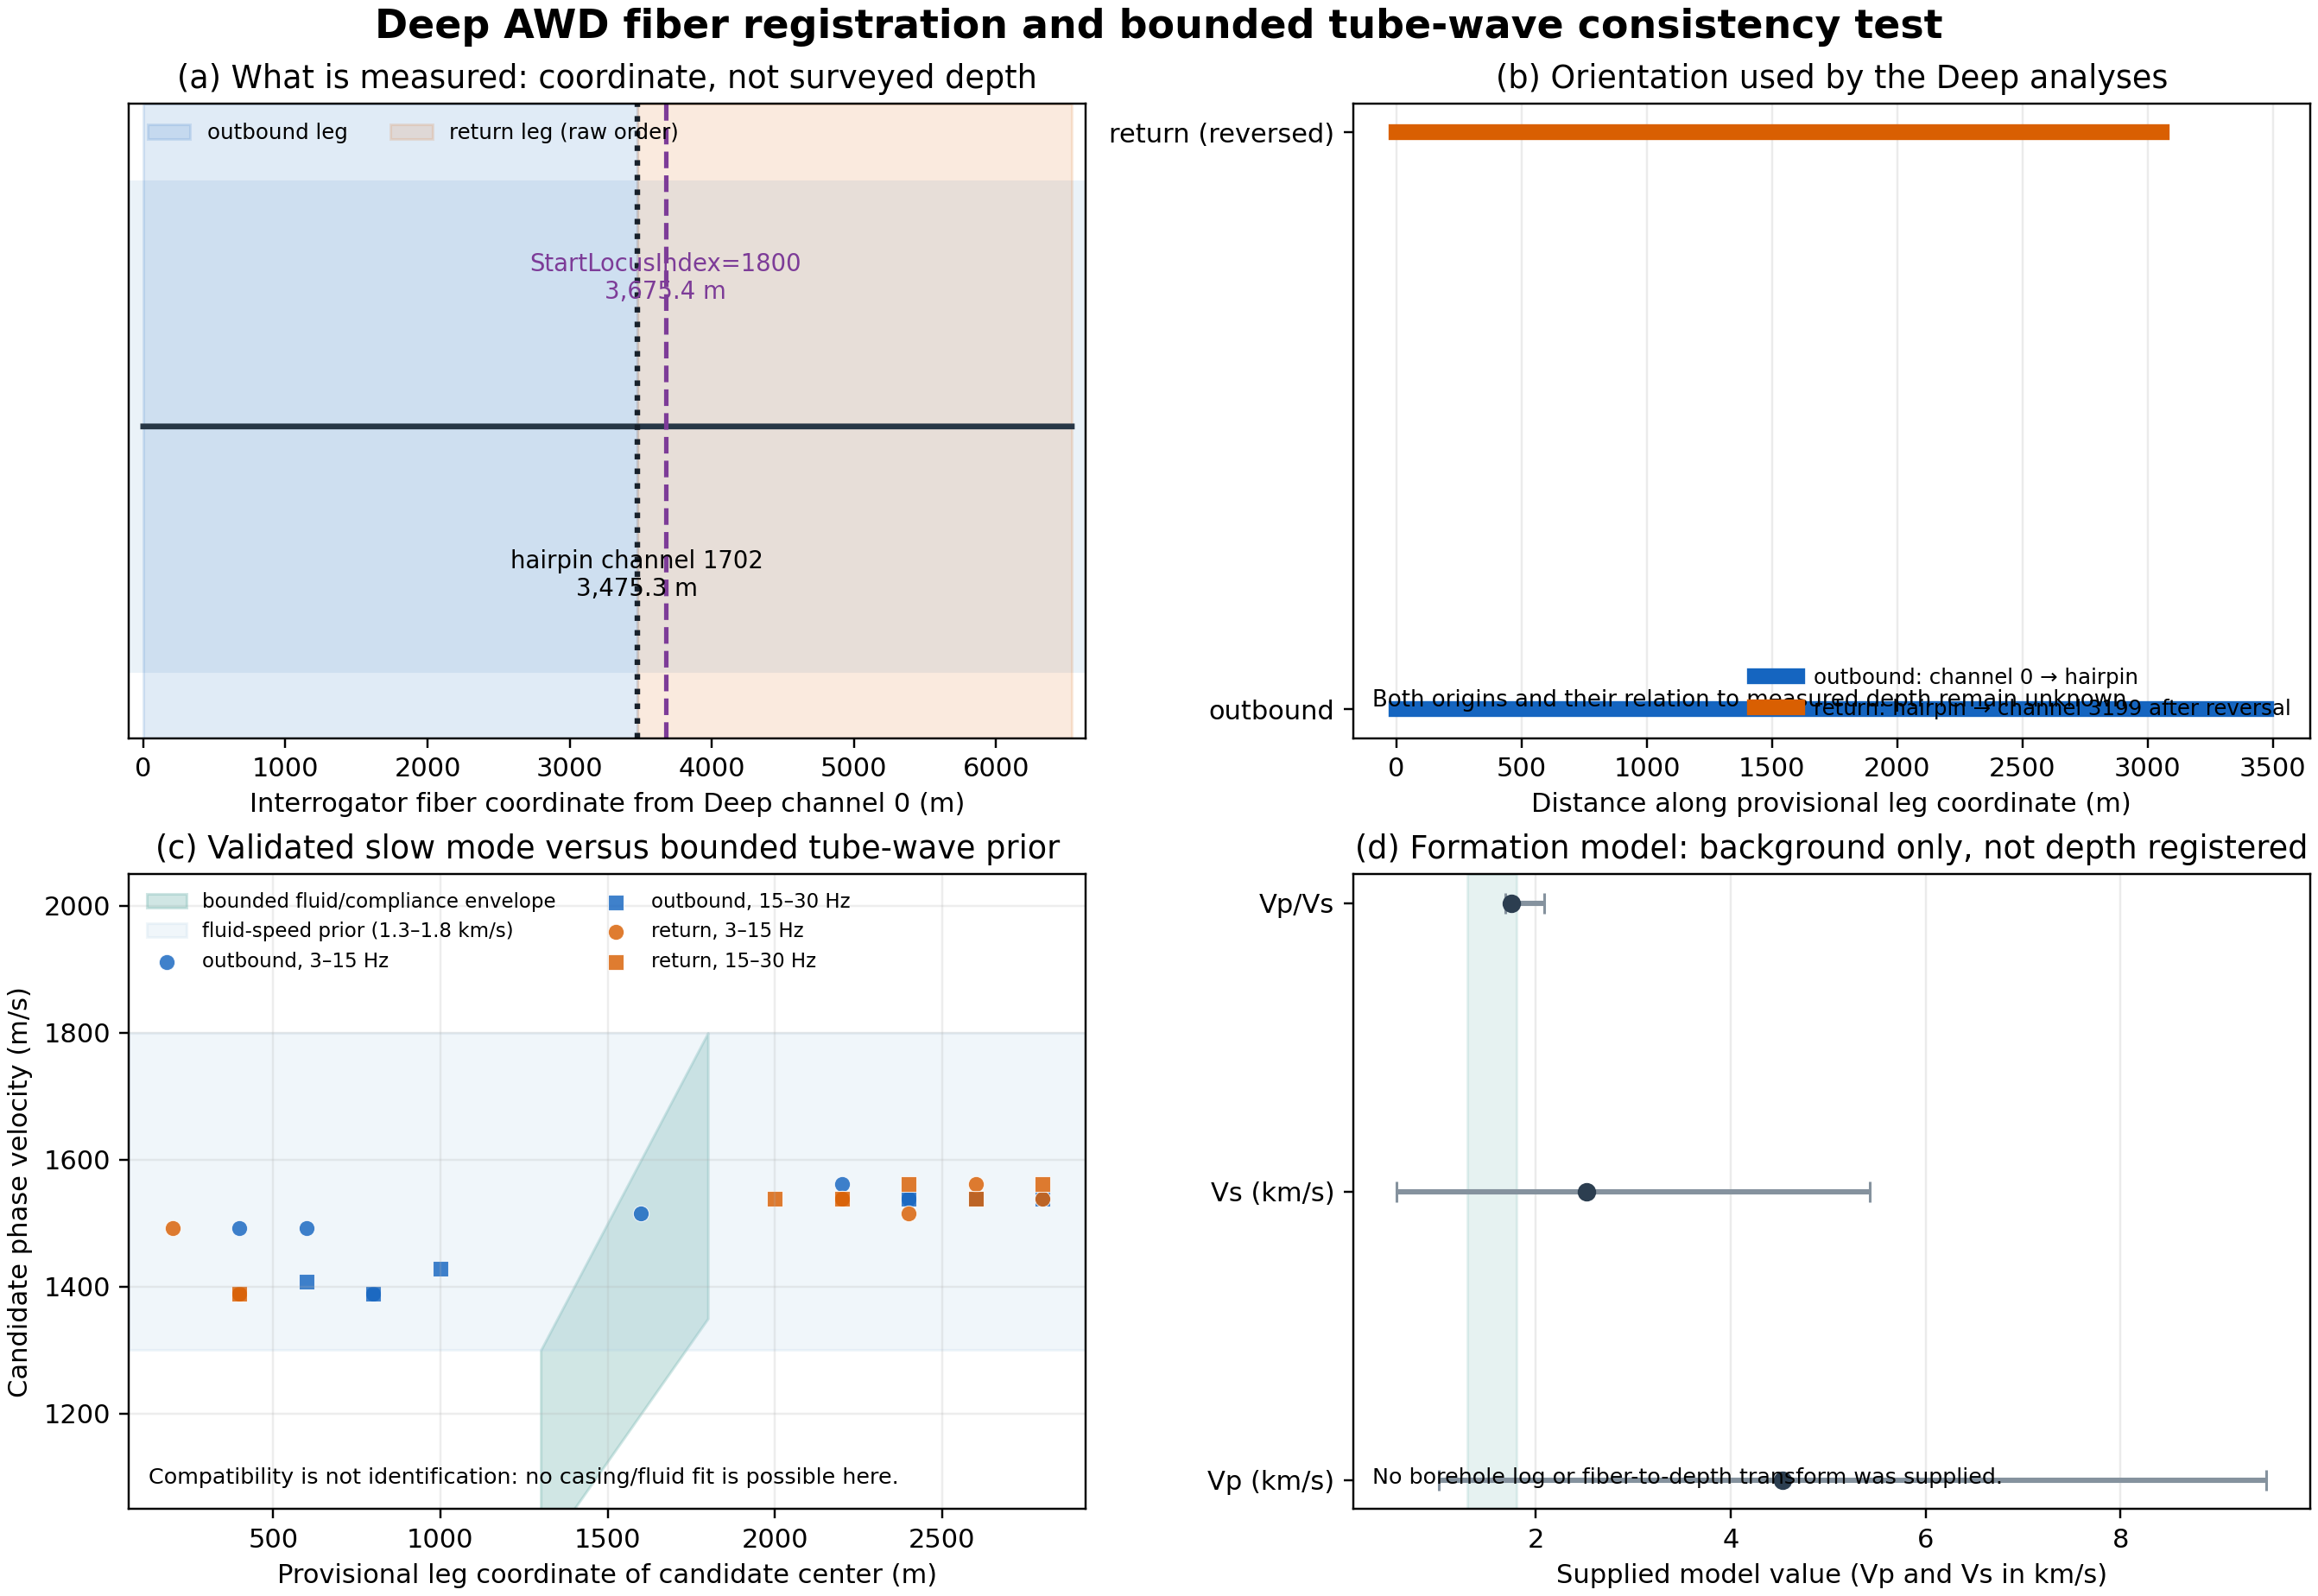
\includegraphics[width=0.98\linewidth]{deep_registration_forward_model.png}
\caption{\textbf{Deep fiber-coordinate registration and bounded tube-wave consistency test.} (a) The complete 3200-locus Deep array is shown in the coordinate actually available from the HDF5/interrogator metadata: channel index multiplied by the 2.0419-m spatial sampling interval. The dashed line marks \code{StartLocusIndex=1800} (3675.42 m in that coordinate system), and the dotted line marks the data-derived hairpin split at channel 1702 (3475.31 m). Neither value is a surveyed measured depth. (b) The outbound and raw-return portions are shown in the provisional orientation used by the Deep signed-slowness analyses; reversing the return traces makes the displayed leg orientation comparable but does not establish a physical downhole direction. (c) The 24 independently validated 1.3--1.8-km-s$^{-1}$ candidates (six per leg and frequency band) are compared with a bounded envelope formed from a 1.3--1.8-km-s$^{-1}$ fluid prior and an explicit 0.75--1.0 phenomenological compliance factor. The candidates have median 1.538 km s$^{-1}$ and 5th--95th percentile 1.389--1.563 km s$^{-1}$, so all lie within the direct fluid prior and the broader envelope. This is a kinematic compatibility test, not a tube-wave dispersion fit or permeability inversion. (d) The transferred SAFOD $V_P$, $V_S$, and $V_P/V_S$ arrays are summarized as a formation-background prior only; the files contain no borehole-log registration or surveyed Deep fiber-to-depth transform. The figure therefore answers what the present metadata permit us to claim---coordinate reproducibility and tube-wave-like speed compatibility---while explicitly ruling out a physical-depth or fracture-location interpretation at this stage.}
\end{figure}

\takeaway{\preliminary: the Deep mode is tube-wave-consistent in speed, but the current files do not register it to measured depth.  Obtain the deployment drawing or surveyed lead-in/turnaround depths and the borehole fluid, casing, and log files before a physical tube-wave model or permeability interpretation.}

\section{Figure 18: Does the delay contain a nonmonotone tidal-timescale component after source-history removal?}
\figquestion{After regressing out source-history and coupling proxies, does the 49-burst Nano delay series contain a reproducible reversible component on a tidal timescale?}

The response is the 49 burst-level leave-one-burst-out Nano delay estimates in
milliseconds relative to their within-burst templates.  Because no independent
ground-level compaction sensor is present in the workspace, the baseline model
uses cumulative AWD drops as a mechanical-history proxy and burst signal RMS as
an observed source-coupling proxy.  A phase-free 24-hour sine/cosine pair is
then added to represent one maximum and one minimum without imposing an
opening/closing sign.  Model improvement is evaluated with five contiguous
time-block cross-validation and a circular three-burst residual bootstrap under
the baseline null.

The baseline blocked-CV RMSE is 0.297 ms; adding the harmonic reduces it to
0.223 ms.  The fitted harmonic amplitude is 0.283 ms, with a maximum near
5.0 h and minimum near 17.0 h relative to the first burst.  The observed
$\Delta$RSS is 0.863 ms$^2$; the naive nested-model p-value is 0.00030 and
the three-burst block-bootstrap p-value is 0.002.  This supports a reproducible
nonmonotone delay component in this 24-hour experiment after the stated nuisance
regression.

This is not yet a tidal-force detection.  The compaction regressor is
cumulative drop history rather than measured ground displacement, and the
harmonic phase is fitted from the data rather than computed from astronomical
tidal potential or fault-normal traction.  The extrema therefore cannot yet be
called fault opening and fault closing.  The physically phased astronomical control is now completed in Figure 20. It uses a scalar
Sun/Moon degree-2 potential; environmental controls, an independent compaction
record, and a fault-normal traction convention remain unavailable.

\begin{figure}[H]
\centering
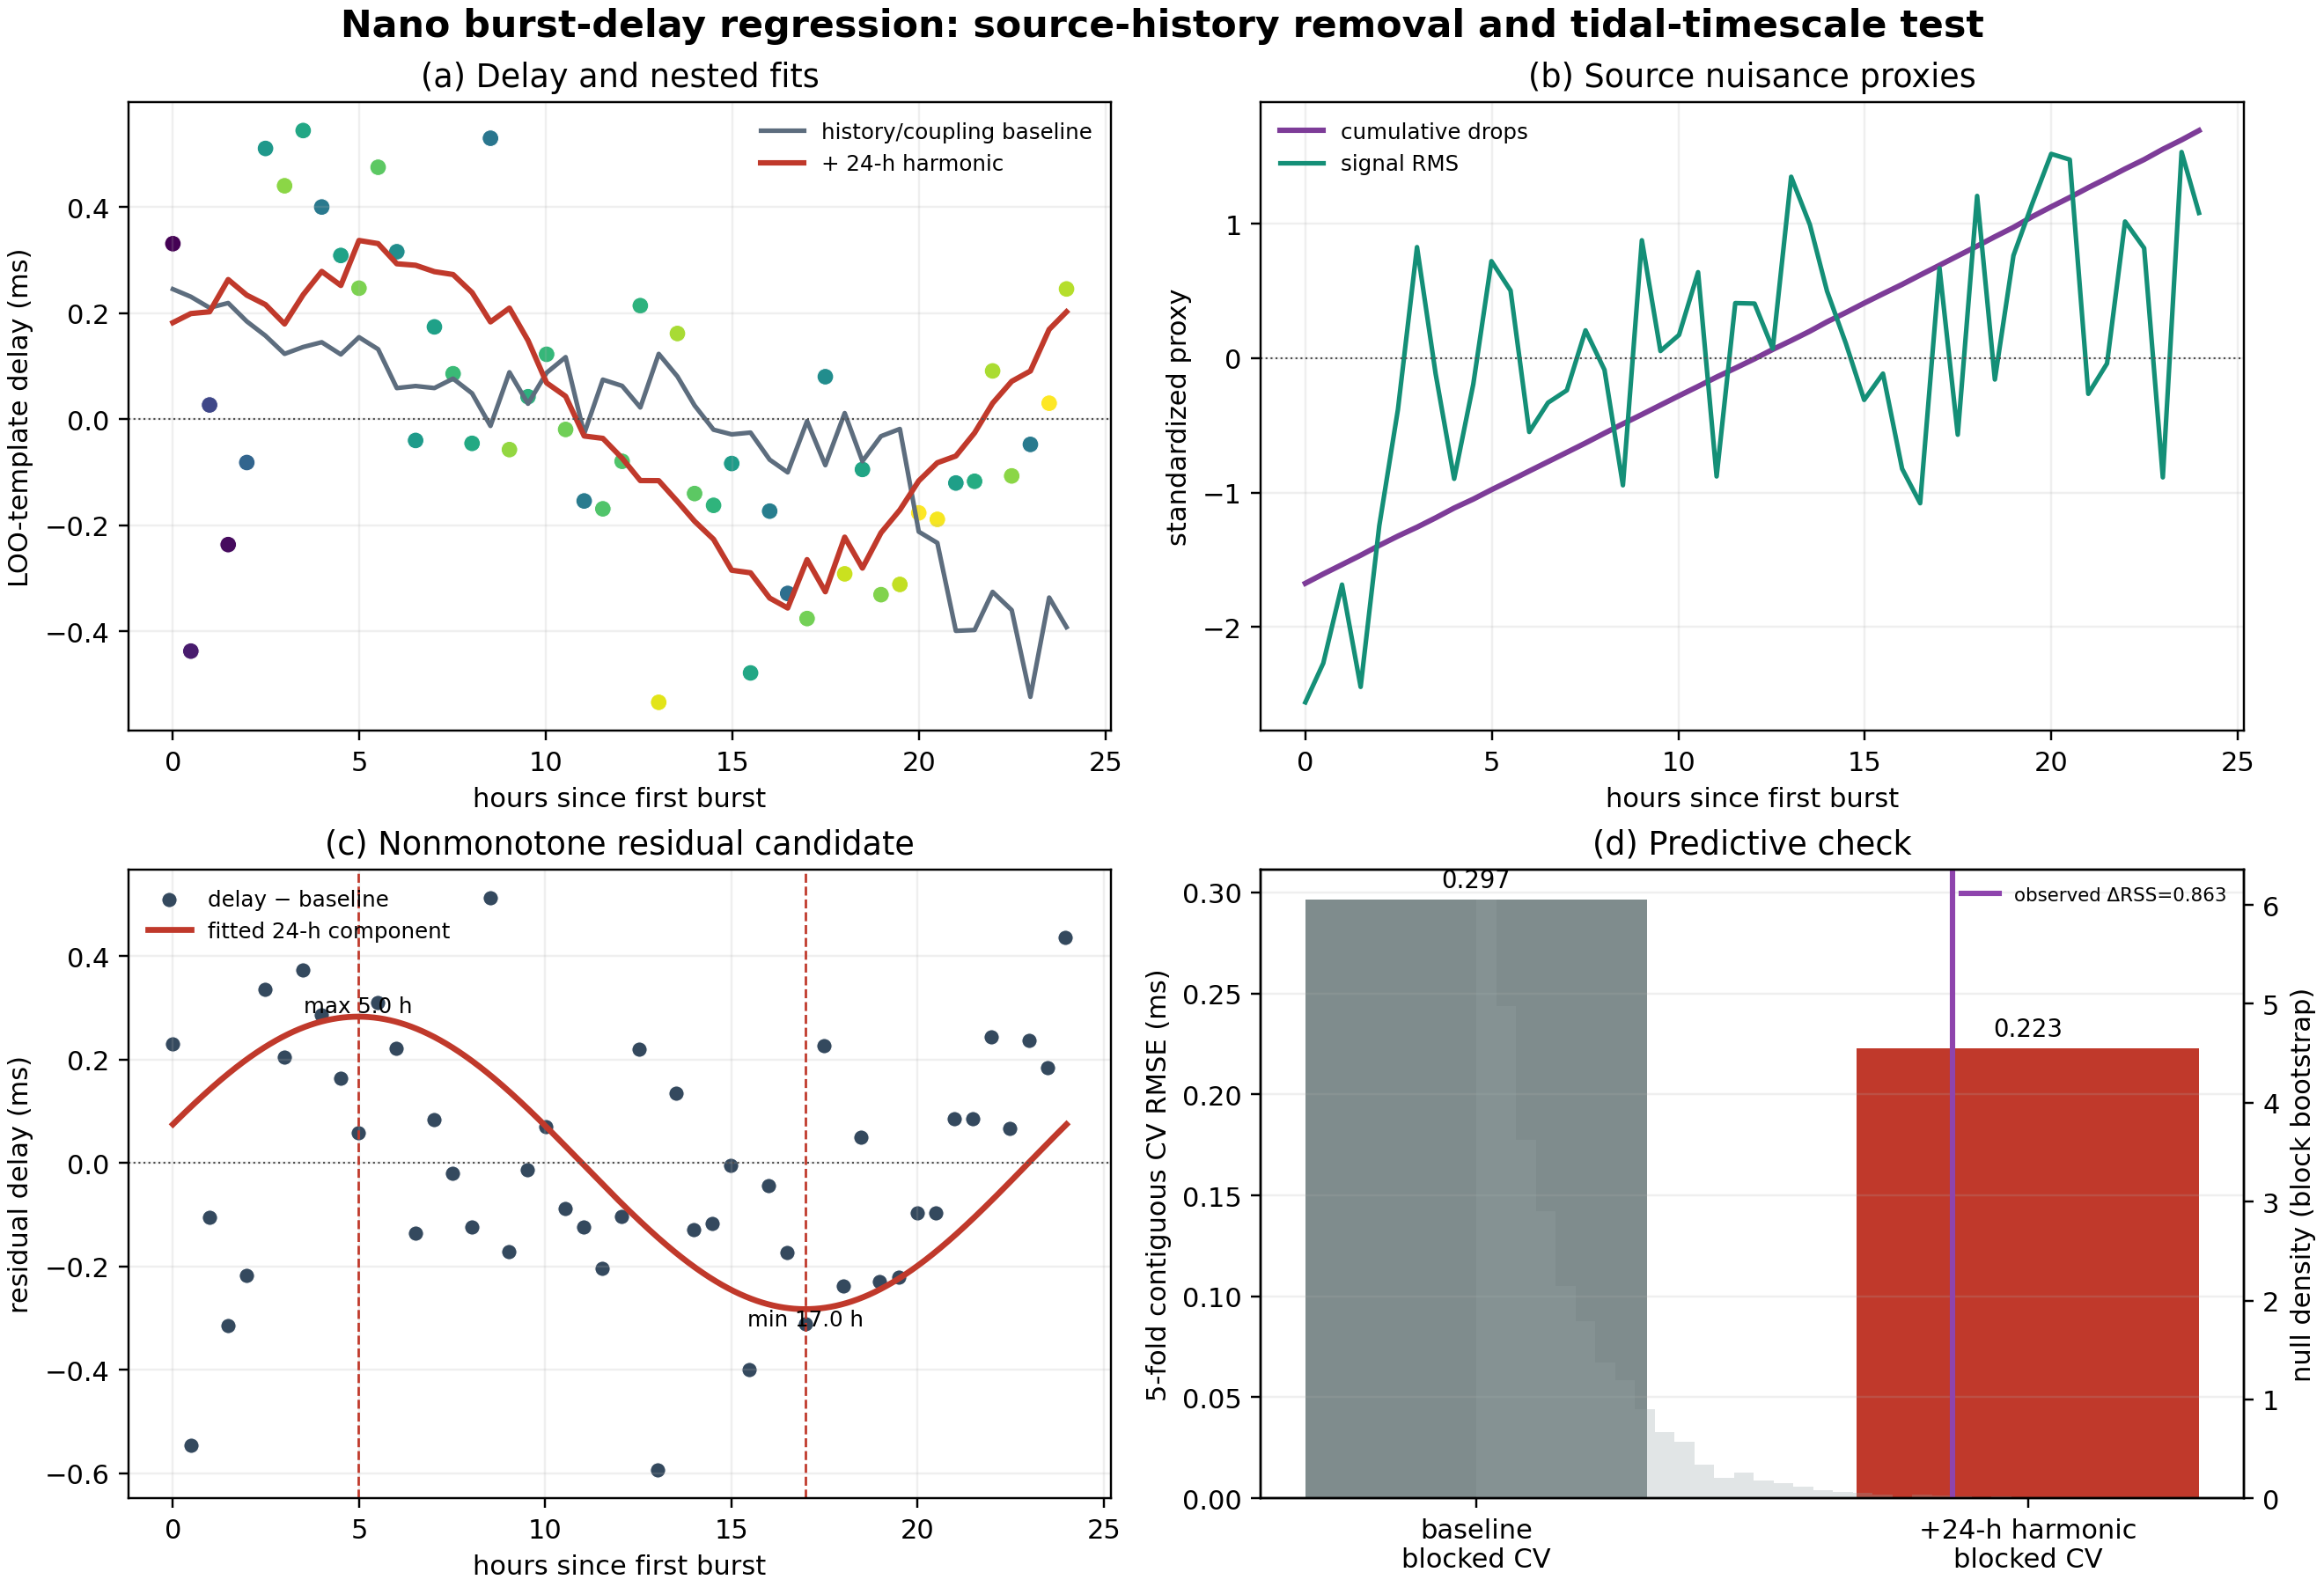
\includegraphics[width=0.98\linewidth]{nano_tidal_compaction_regression.png}
\caption{\textbf{Source-history regression and nonmonotone tidal-timescale delay test.} (a) Points show the 49 burst-level leave-one-burst-out Nano delay estimates relative to their within-burst templates; color denotes standardized burst signal RMS. The gray curve is the baseline regression on cumulative AWD-drop history and coupling proxy, while the red curve adds a phase-free 24-hour sine/cosine pair. (b) The two nuisance covariates are shown after standardization: cumulative drop count represents mechanical source history, and burst signal RMS represents observed source coupling. Neither is an independent ground-level compaction measurement. (c) Residual delays after removal of the baseline are compared with the fitted 24-hour component. The fitted component has amplitude 0.283 ms, a maximum at approximately 5.0 h, and a minimum at approximately 17.0 h relative to the first burst, showing the requested nonmonotone form without assigning a physical opening/closing sign. (d) Five contiguous-block cross-validation gives RMSE 0.297 ms for the baseline and 0.223 ms after adding the harmonic. The inset null distribution is generated by circular three-burst residual bootstrap under the baseline model; the observed $\Delta$RSS is 0.863 ms$^2$ and the bootstrap exceedance probability is 0.002. The result is a candidate tidal-timescale delay pattern, not a detection of Earth tide or fault opening/closing; the physically phased astronomical control is evaluated in Figure 20; its weaker result does not support that interpretation.}
\end{figure}

\takeaway{\preliminary: source-history removal leaves a reproducible nonmonotone 24-hour-timescale delay component.  Do not label its extrema as fault opening or closing until an external tide/traction predictor supplies the physical phase and sign.}

\section{Figure 19: Does CCA recover the tidal-timescale pattern?}
\figquestion{Does a multivariate canonical-correlation analysis recover a shared pattern between the phase-free tidal-timescale basis and source-corrected delay/coupling observables?}

The predictor set contains sine/cosine pairs at 24.0 h and 12.4206 h, allowing
CCA to choose a phase-free diurnal/semidiurnal combination.  The response set
contains the Nano delay after cumulative-drop and signal-RMS baseline correction
and standardized burst signal RMS.  CCA finds the linear combinations of the
two sets with maximum correlation.  Independent row permutations provide a
simple null; permutations of three-burst blocks preserve some serial structure.
Five contiguous time folds test whether the canonical association generalizes.
Absolute held-out correlations are reported because canonical signs can flip
between folds.

The full 49-burst sample gives a first canonical correlation of 0.533.  The
independent row-permutation p-value is 0.019, but the three-burst
block-permutation p-value is 0.118.  The five contiguous-fold absolute
correlations are 0.697, 0.016, 0.378, 0.057, and 0.075, with median 0.075.
CCA therefore identifies an exploratory full-sample association with the
phase-free tidal-timescale basis, but the serially aware null and unstable
held-out correlations do not establish a robust tidal signal.

CCA cannot supply the missing physical phase or opening/closing sign, and the
response still uses proxy-based source correction.  The physically phased follow-up is reported in Figure 20. It is a stricter
external-phase control, not a fault-traction calculation: the scalar potential
does not specify opening versus closing, and the response still uses proxy-based
source correction. The current canonical variate is not a fault-opening measurement.

\begin{figure}[H]
\centering
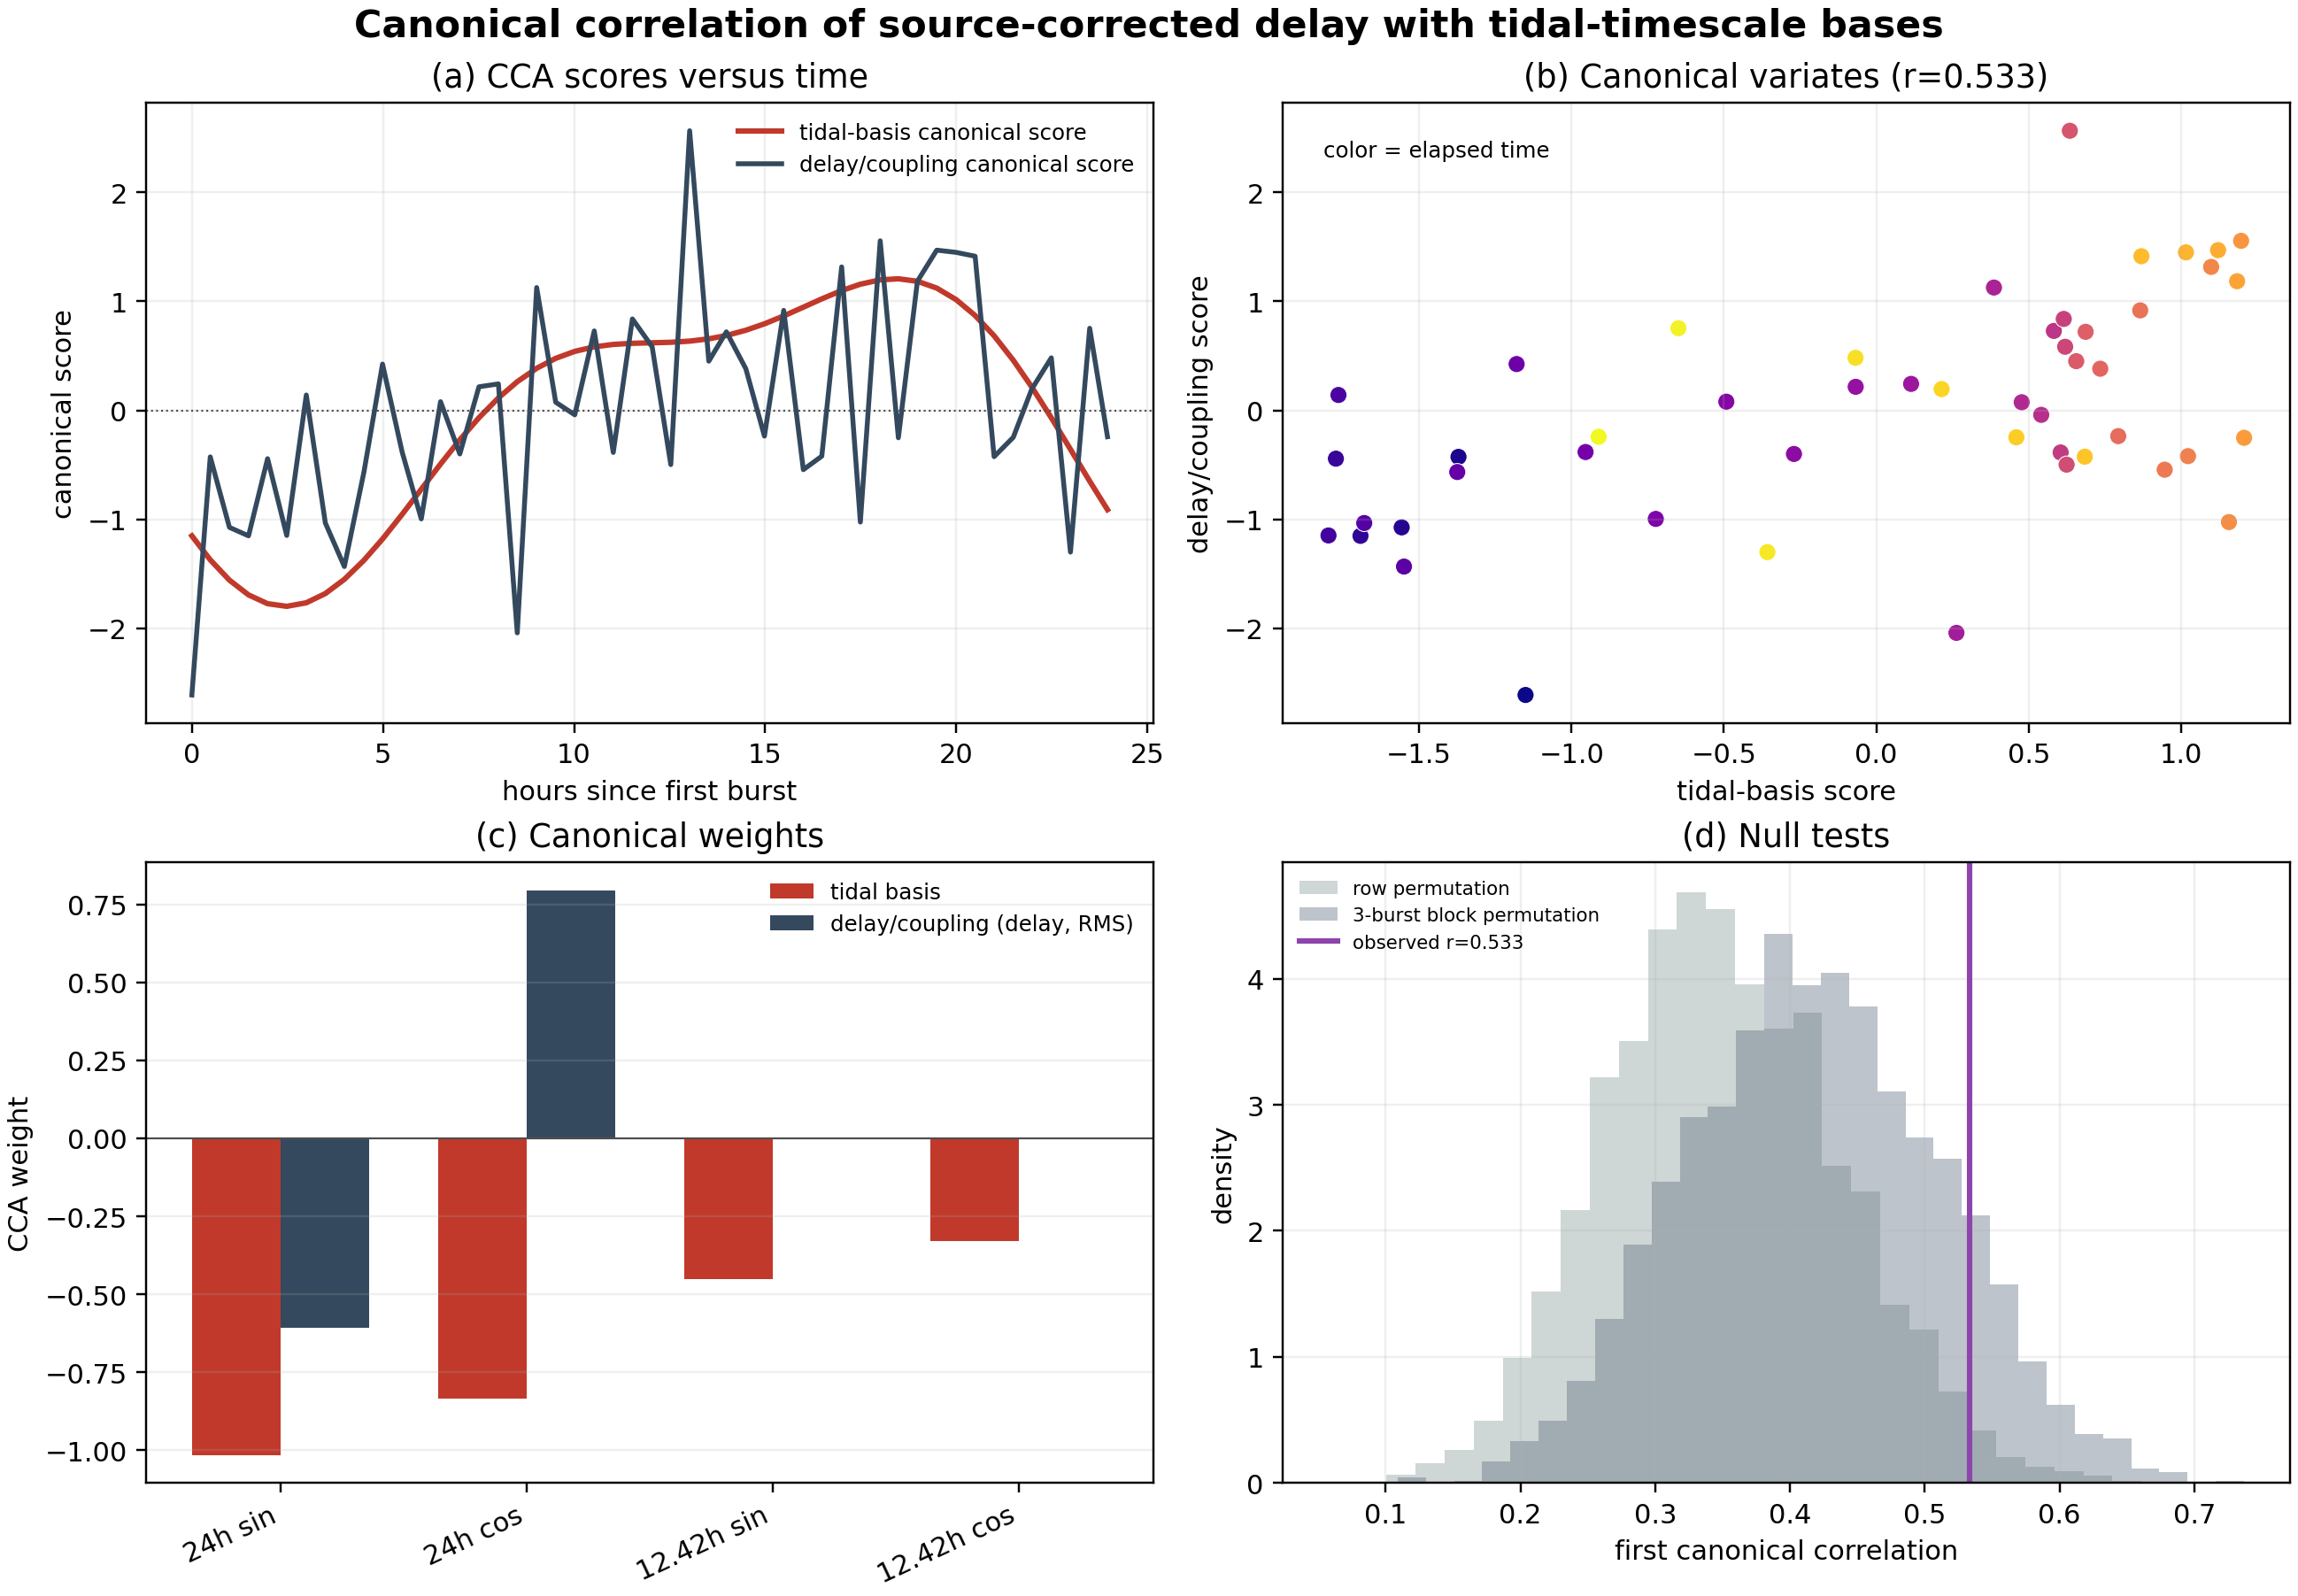
\includegraphics[width=0.98\linewidth]{nano_tidal_cca.png}
\caption{\textbf{Exploratory canonical correlation between tidal-timescale bases and corrected Nano observables.} (a) The first canonical scores are shown against elapsed time for the phase-free predictor set (24.0- and 12.4206-hour sine/cosine bases) and the response set (source-corrected delay plus burst signal RMS). (b) Their full-sample canonical variates have correlation 0.533; color denotes elapsed time. (c) Bars show the canonical weights for the four temporal basis functions and the two response variables (delay and RMS). (d) The observed correlation is compared with two null distributions: independent row permutations and serial-dependence-aware permutations of three-burst blocks. The row-permutation p-value is 0.019, whereas the block-permutation p-value is 0.118. Five contiguous held-out folds produce absolute correlations 0.697, 0.016, 0.378, 0.057, and 0.075, demonstrating instability across time. The CCA therefore finds an exploratory full-sample association but does not establish a robust tidal signal, physical tide phase, fault opening/closing, or causation.}
\end{figure}

\takeaway{\preliminary: the phase-free CCA is not confirmed by serially aware controls; the externally phased physical-potential control in Figure 20 is weaker and does not support a tidal opening/closing interpretation.}

\section{Figure 20: Does an externally phased astronomical predictor reproduce it?}
\figquestion{Does the source-corrected Nano delay/coupling response align with an astronomical predictor whose phase is fixed by the actual UTC burst times, rather than fitted from the delay series?}

The phase-free 24-hour harmonic and exploratory CCA are useful pattern-discovery
results, but they allow the delay data to choose the phase.  Figure 20 is the
stricter control.  For each of the 49 burst times, the analysis evaluates a
low-precision geocentric Sun/Moon ephemeris and the degree-2 tide-generating
potential at approximate SAFOD latitude $35.98^{\circ}$ N and longitude
$120.55^{\circ}$ W.  The Moon and Sun potentials form the predictor set; they
are not fitted sine/cosine phases.  The response set is unchanged: the Nano
burst delay after cumulative-drop and burst-RMS source-history correction,
plus burst signal RMS.

The first canonical correlation is $r=0.366$.  Independent row permutations
give $p=0.116$ and three-burst block permutations give $p=0.263$.  Five
contiguous held-out folds give absolute correlations $0.780$, $0.247$,
$0.230$, $0.501$, and $0.039$ (mean $0.359$, median $0.247$).  Thus the
phase-free candidate is not reproduced as a stable, externally phased
astronomical response.  This is a negative control on the tidal interpretation,
not evidence against the existence of a delay pattern.

The predictor is a scalar degree-2 potential, not a fault-normal traction.  No
independent source-ground compaction/settlement series was found, and no
surveyed fault orientation or stress convention is available.  Consequently
this figure cannot assign an opening/closing sign, identify a hydraulic
fracture, or establish a tidal-force detection.  A precision strain/traction
rerun is conditional on those missing external inputs.

\begin{figure}[H]
\centering
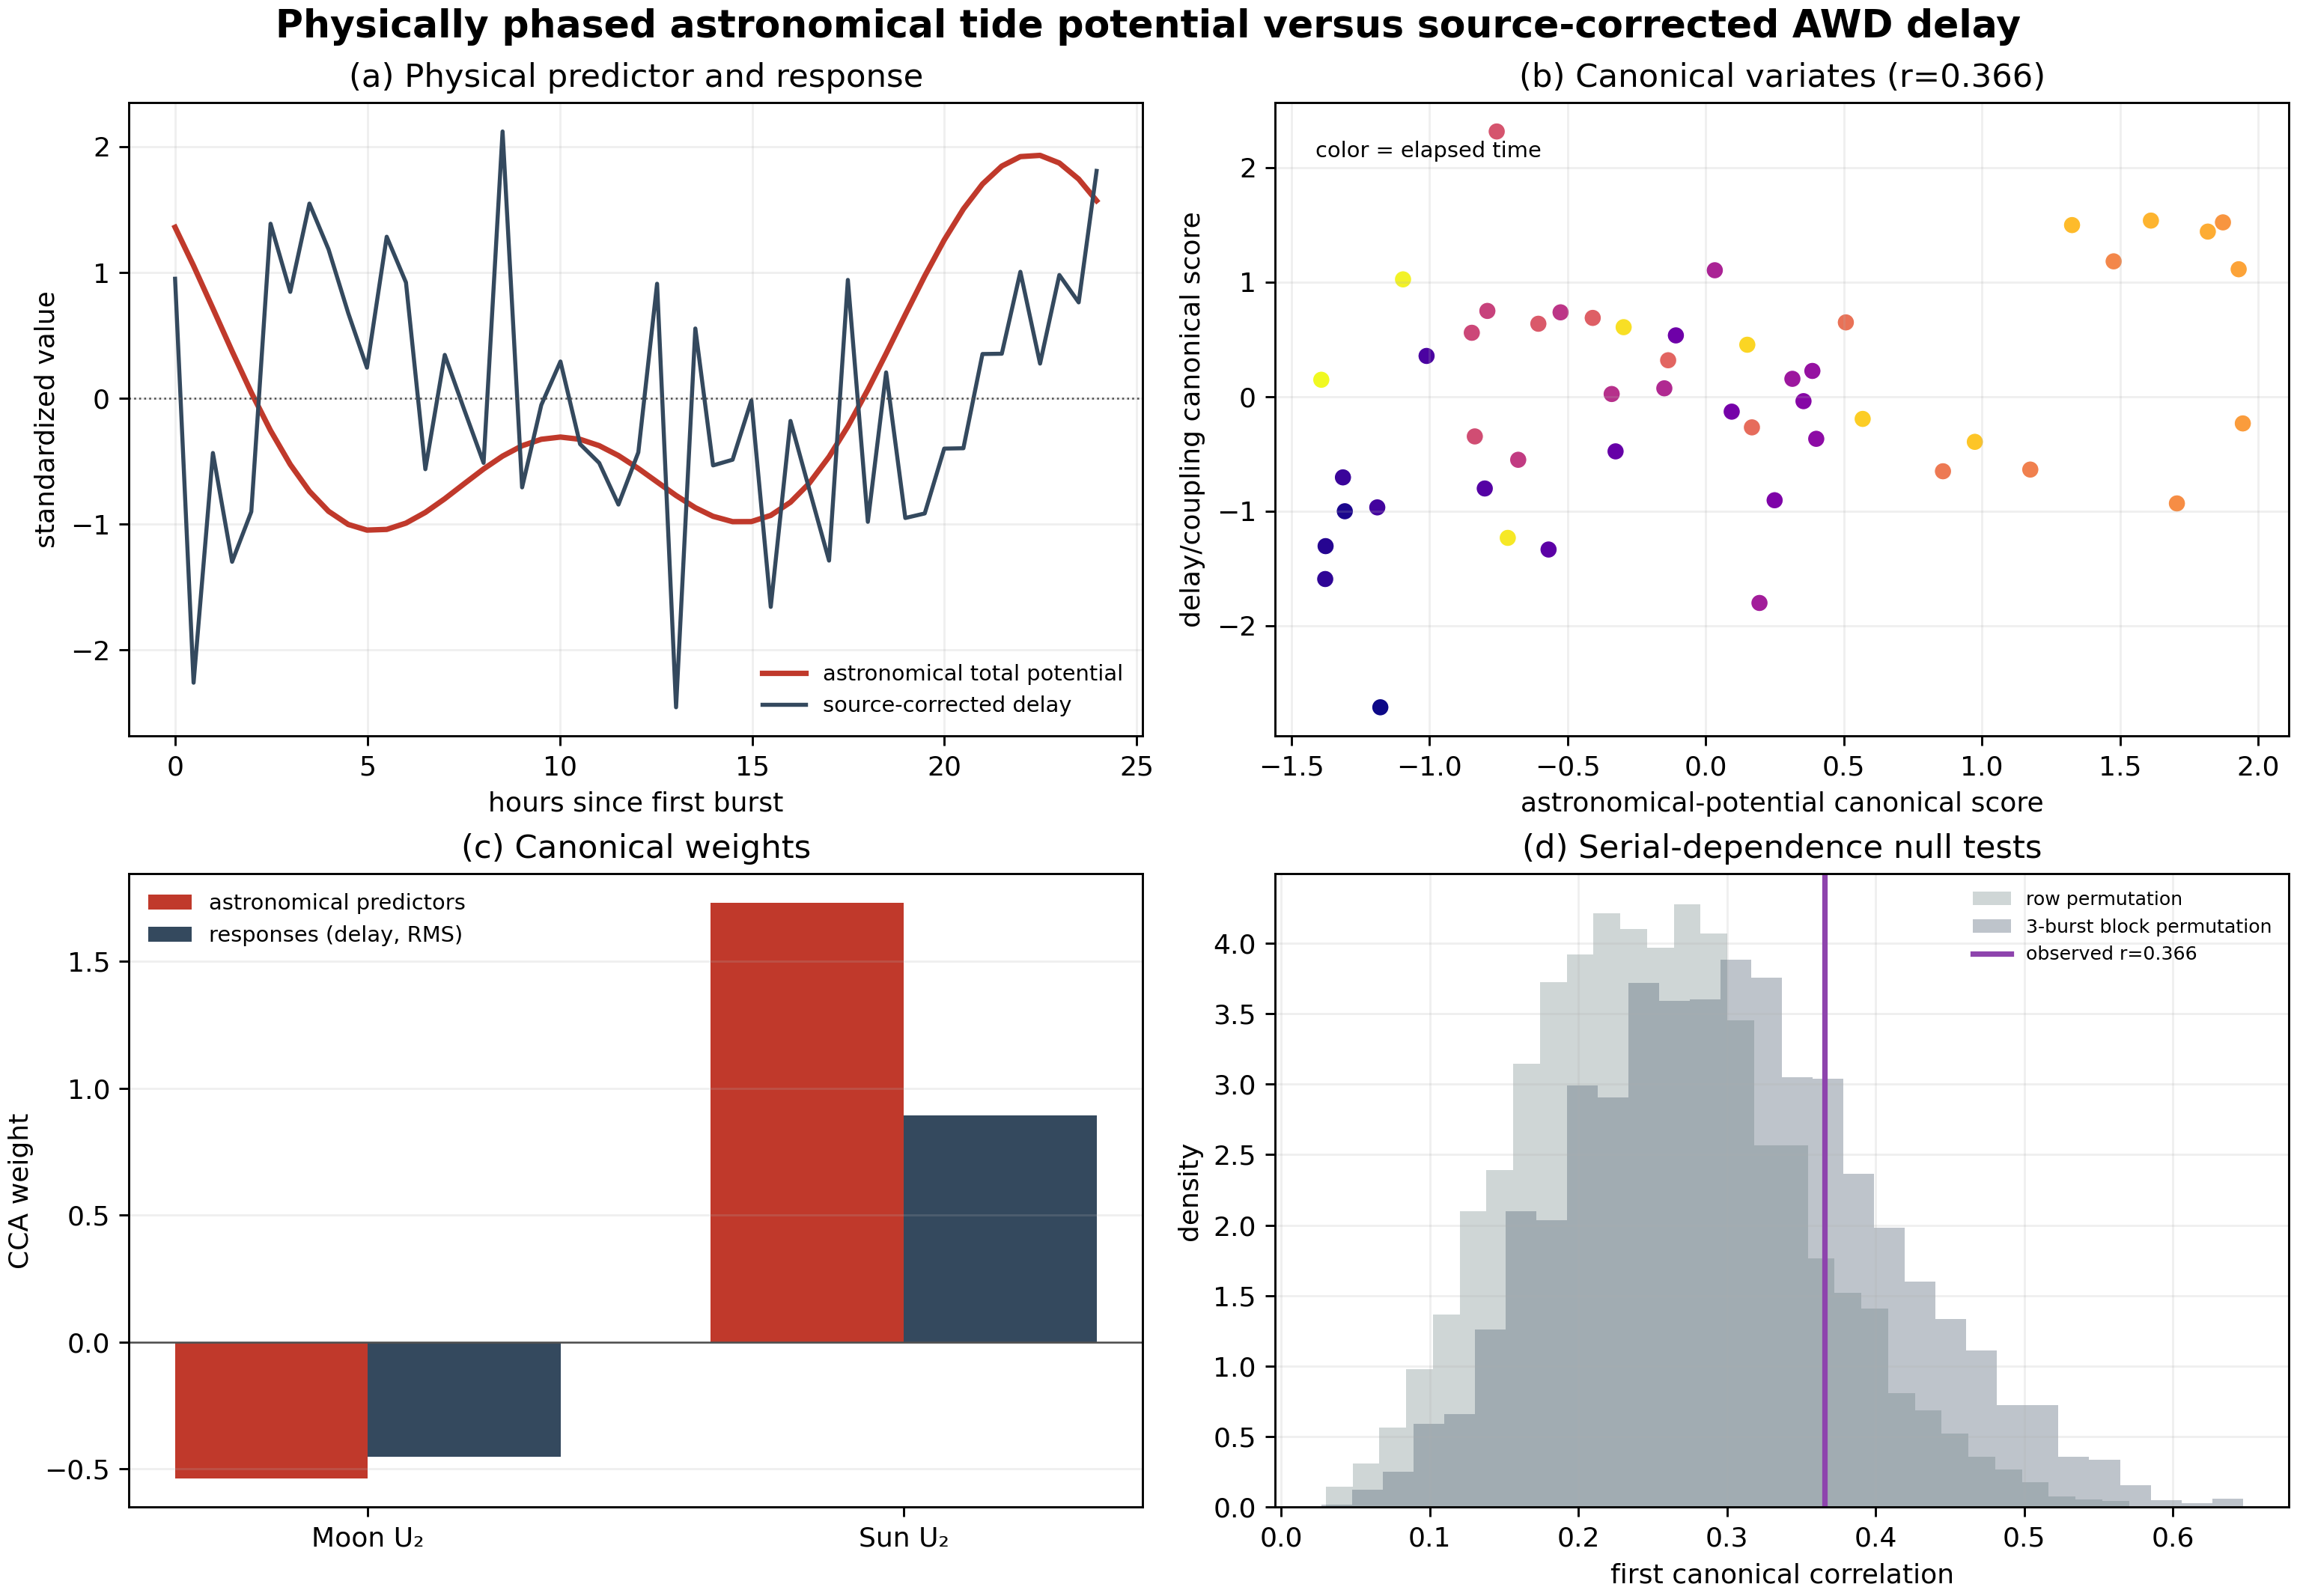
\includegraphics[width=0.98\linewidth]{nano_physical_tide_cca.png}
\caption{\textbf{Physically phased astronomical tide-potential CCA as a control on the fitted tidal-timescale pattern.} The 49 burst times are the UTC medians of the AWD manifest; no phase is fitted to the delay series. (a) Standardized low-precision degree-2 Moon-plus-Sun tide-generating potential at approximate SAFOD latitude $35.98^{\circ}$ N, longitude $120.55^{\circ}$ W is compared with the source-corrected Nano delay. The potential is a scalar timing/forcing proxy, not fault-normal traction. (b) First canonical variates of the Moon and Sun potentials and the response pair (corrected delay and burst RMS), colored by elapsed time. (c) Canonical weights for the two body-specific predictors and the response variables. (d) Observed $r=0.366$ versus independent row and serial-dependence-aware three-burst block nulls. Row-permutation $p=0.116$ and block-permutation $p=0.263$ do not provide a robust detection. Five contiguous held-out folds give absolute correlations $0.780$, $0.247$, $0.230$, $0.501$, and $0.039$, demonstrating temporal instability. The physical-phase control therefore does not confirm the earlier phase-free harmonic as an astronomical-tide response; no opening/closing sign is assigned.}
\end{figure}

\takeaway{\preliminary: the externally phased control weakens the tidal interpretation.  The candidate delay pattern remains a source-history/environment question, not a demonstrated fault-opening signal.}

\section{Figure 21: Is the Deep slow mode observable at the provisional deforming-strand depths?}
\figquestion{If the plausible surface-lead-in interpretation is used provisionally, does the repeatable Deep slow mode persist in windows covering the SDZ and CDZ?}

This is the first direct test of the proposed downhole-baseline story.  It is
not a creep-rate measurement: the present record spans one day, whereas aseismic
creep accumulates over much longer intervals.  The purpose is to establish
whether a repeatable observable exists at the target interval before requesting
repeat surveys or attempting a casing-deformation forward model.

The scan uses 200-m windows sampled every 50 m across provisional 3000--3450 m.
Outbound coordinate is mapped as $s_{\rm out}=\mathrm{depth}$; after reversing
the return leg, its coordinate is mapped as $s_{\rm return}=3475.31-
\mathrm{depth}$~m.  This assumes the interrogator lead-in is surface cable and
that the data-derived hairpin coordinate is the turnaround depth.  Neither
assumption is surveyed in the present files, so every depth in this section is
explicitly provisional.  Odd non-empty epochs select signed slowness and arrival
time, and even epochs validate the fixed trajectory.  The two frequency bands
(3--15 and 15--30 Hz) and both slowness signs are retained; 499 channel-order
permutations are used at the two strand depths.

The result is specific.  At both assumed strand depths, the positive 15--30-Hz
branch validates on both the outbound and reversed-return legs: all four explicit
channel-order tests give $p=0.002$.  The 3--15-Hz control is weak, while isolated
negative-direction p-values do not form a coherent opposing branch.  Thus the
slow observable is present in the target windows under the mapping hypothesis.
That is evidence for target-window observability, not a measured tube-wave
reflection, casing deformation, permeability anomaly, or creep signal.

\begin{figure}[H]
\centering
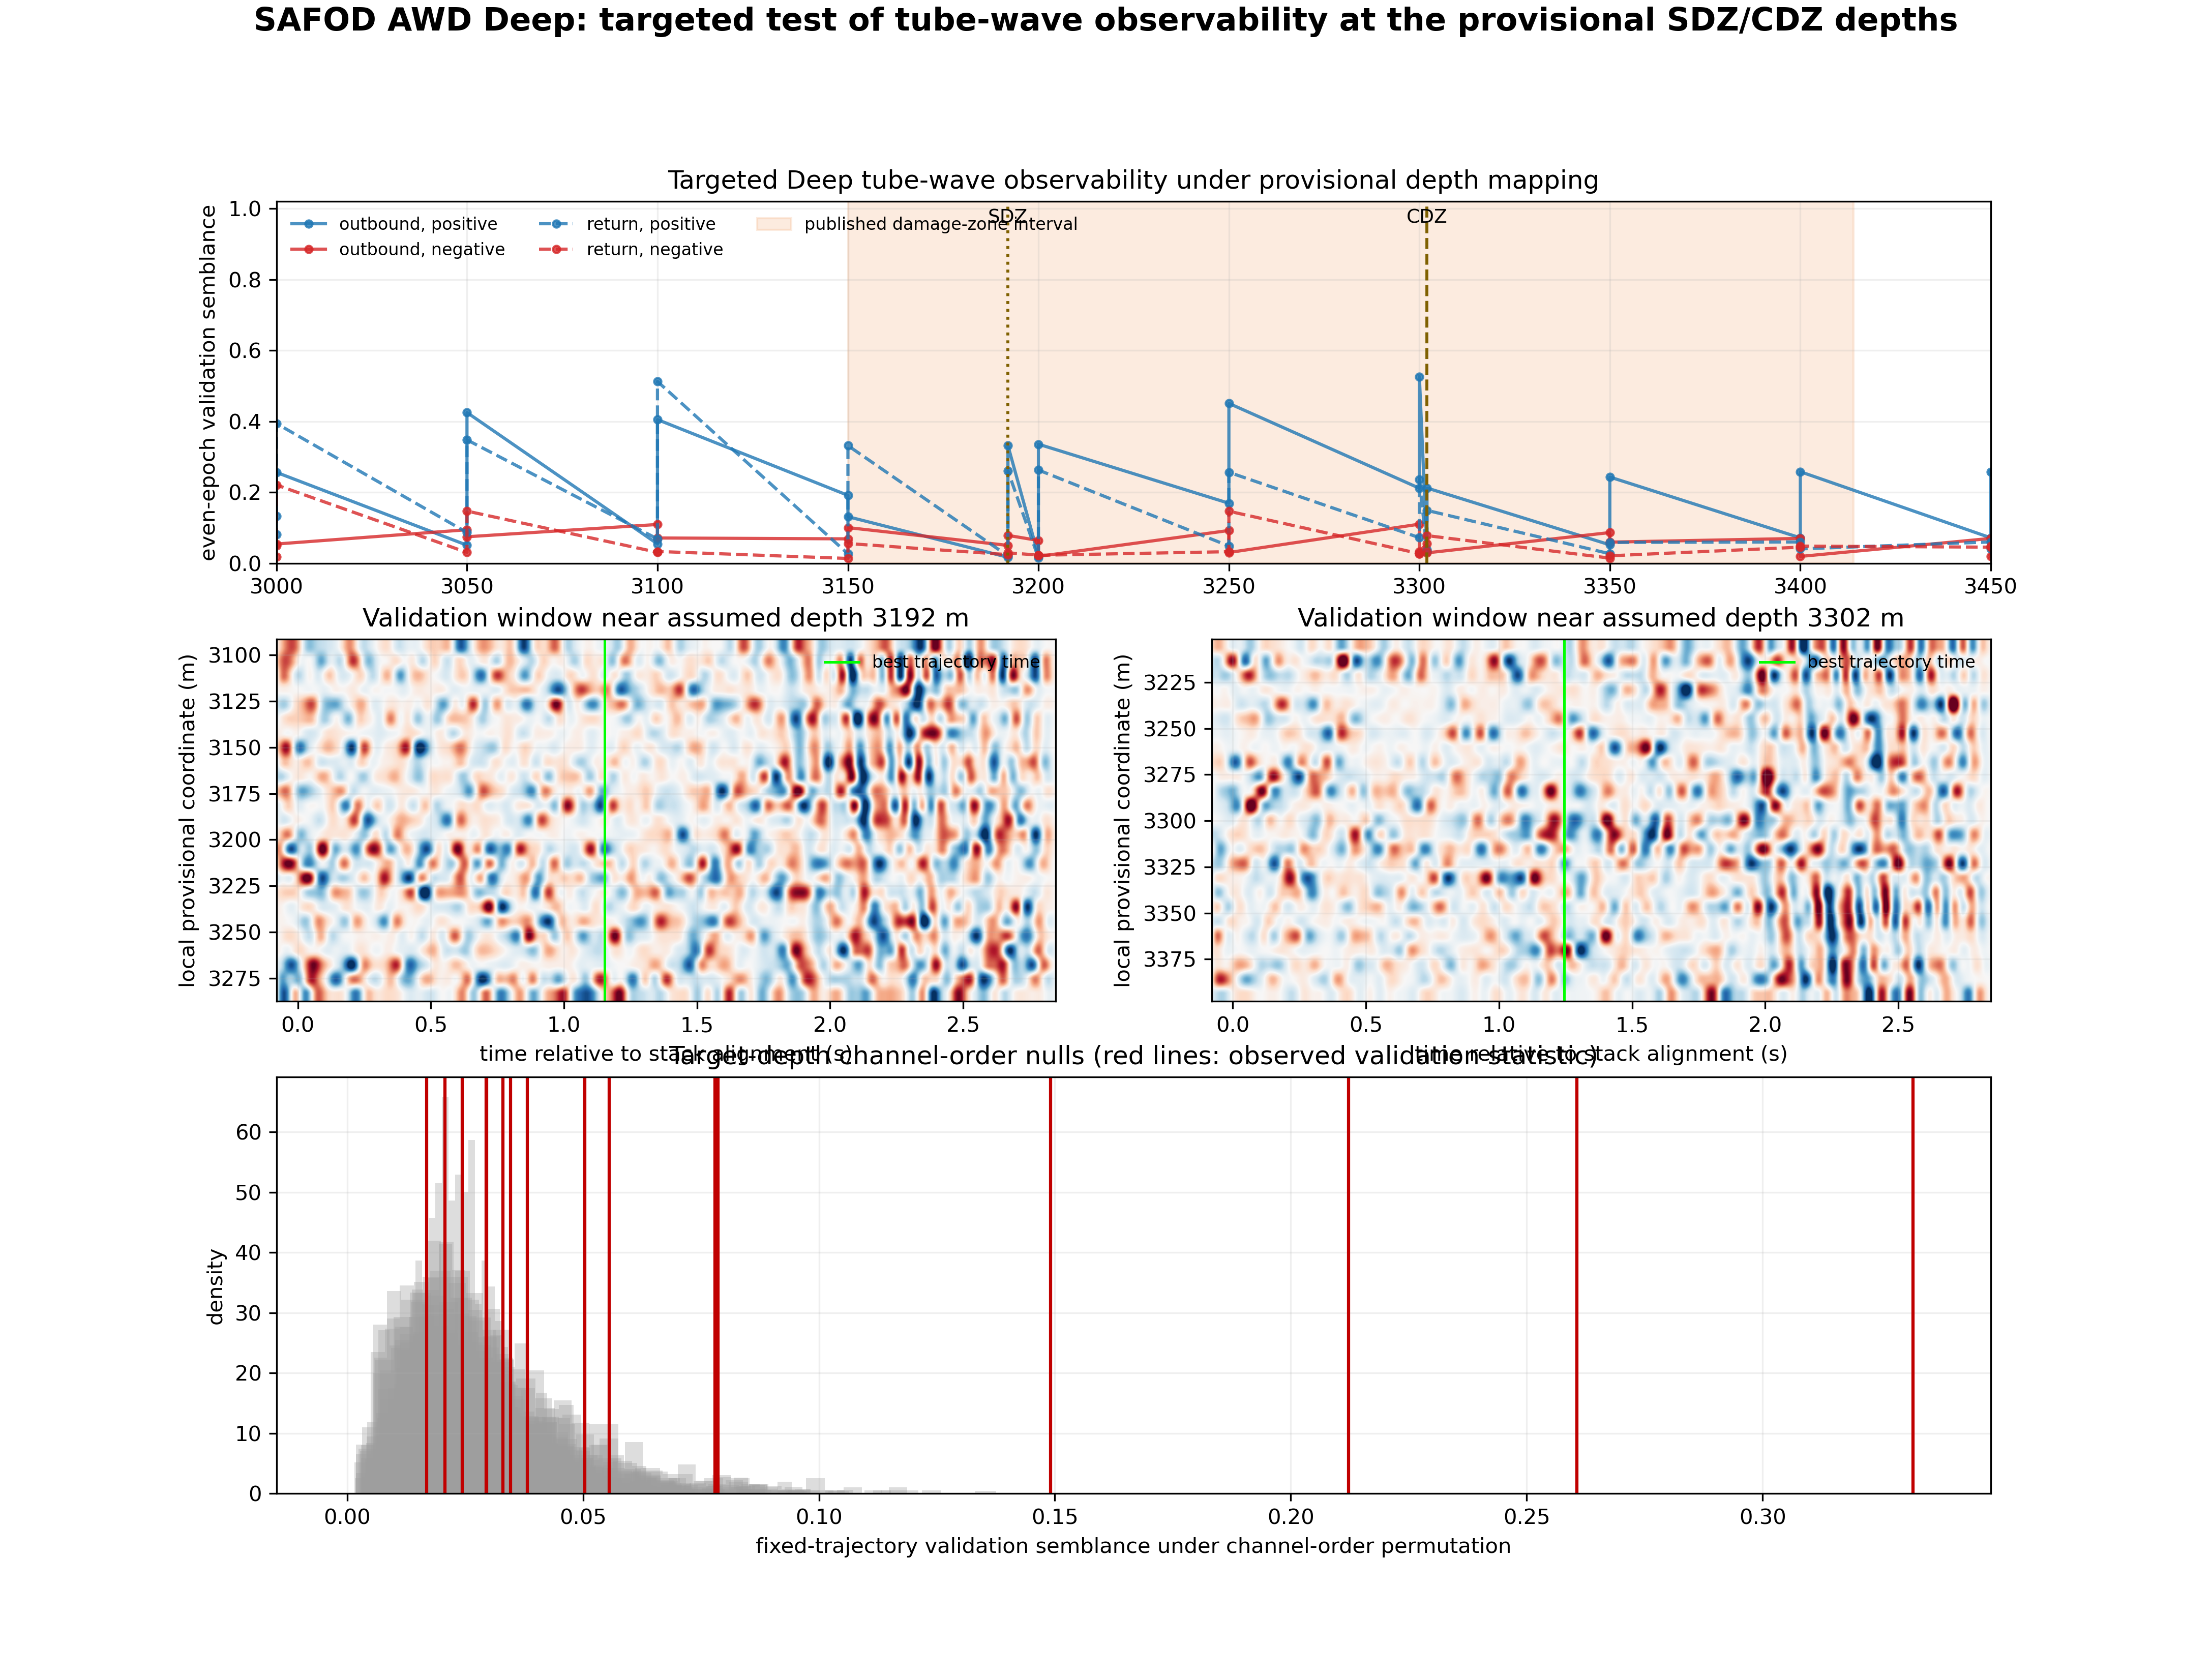
\includegraphics[width=0.98\linewidth]{deep_target_scan.png}
\caption{\textbf{Targeted Deep tube-wave observability at the provisional SAFOD deforming-strand depths.} The upper panel plots even-epoch validation semblance for 200-m Deep windows sampled every 50 m across the provisional 3000--3450-m interval. Solid curves are the outbound leg and dashed curves are the reversed-return leg; blue and red distinguish positive and negative signed slowness. The orange band marks the independently reported 3150--3414-m damage-zone interval, while vertical markers identify the provisional SDZ (3192 m) and CDZ (3302 m). The middle panels show display-scaled validation record sections for windows near those two depths; scaling is applied only for visualization and does not enter the coherence statistics. The lower panel overlays the 499 channel-order permutation distributions for the explicit strand-depth tests; red lines mark the observed fixed-trajectory validation statistics and labels report empirical tail probabilities. The positive 15--30-Hz branch is validated at both provisional strand depths on both legs (each explicit test gives $p=0.002$), whereas the 3--15-Hz control is weak and the isolated negative-direction results are not a coherent opposing branch. The mapping $s_{\rm out}=\mathrm{depth}$ and $s_{\rm return}=3475.31-\mathrm{depth}$ assumes a surface lead-in and a turnaround at 3475.31 m; neither assumption is independently surveyed. Accordingly, this figure establishes target-window observability under a stated registration hypothesis, not a measured reflection, casing deformation, permeability anomaly, or creep rate.}
\end{figure}

\takeaway{\preliminary: the Deep slow mode is observable in the provisional SDZ/CDZ windows in the 15--30-Hz band under the stated coordinate mapping.  Obtain deployment/depth documentation and repeat-survey data before calling this a deformation-monitoring measurement.}

\section{Figure 22: Does the Deep target observable repeat in individual bursts?}
\figquestion{Does the target-window signal recur in held-out AWD bursts, rather than appearing only after epoch stacking?}

The target-depth scan established that the positive 15--30-Hz Deep branch is
observable under a provisional coordinate mapping.  The next requirement for a
useful active-source baseline is burst-level repeatability.  Fixed trajectories
selected from the discovery subset are therefore evaluated independently in all
46 non-empty Deep burst stacks; the 23 even-numbered bursts are treated as
held-out validation observations.

The statistic is positive-minus-negative fixed-trajectory semblance.  It tests
spatial ordering and direction, not absolute amplitude.  At the assumed SDZ,
the positive 15--30-Hz branch occurs in 21/23 outbound and 20/23 return
validation bursts.  At the assumed CDZ it occurs in 21/23 outbound and 16/23
return bursts.  The one-sided sign-test p-values are $3.3\times10^{-5}$,
$2.4\times10^{-4}$, $3.3\times10^{-5}$, and $0.047$, respectively.  Similar
outbound coherence in control windows shows that the result is a repeatable
mode passing through the target interval, not yet a strand-localized casing-
deformation signature.

\begin{figure}[H]
\centering
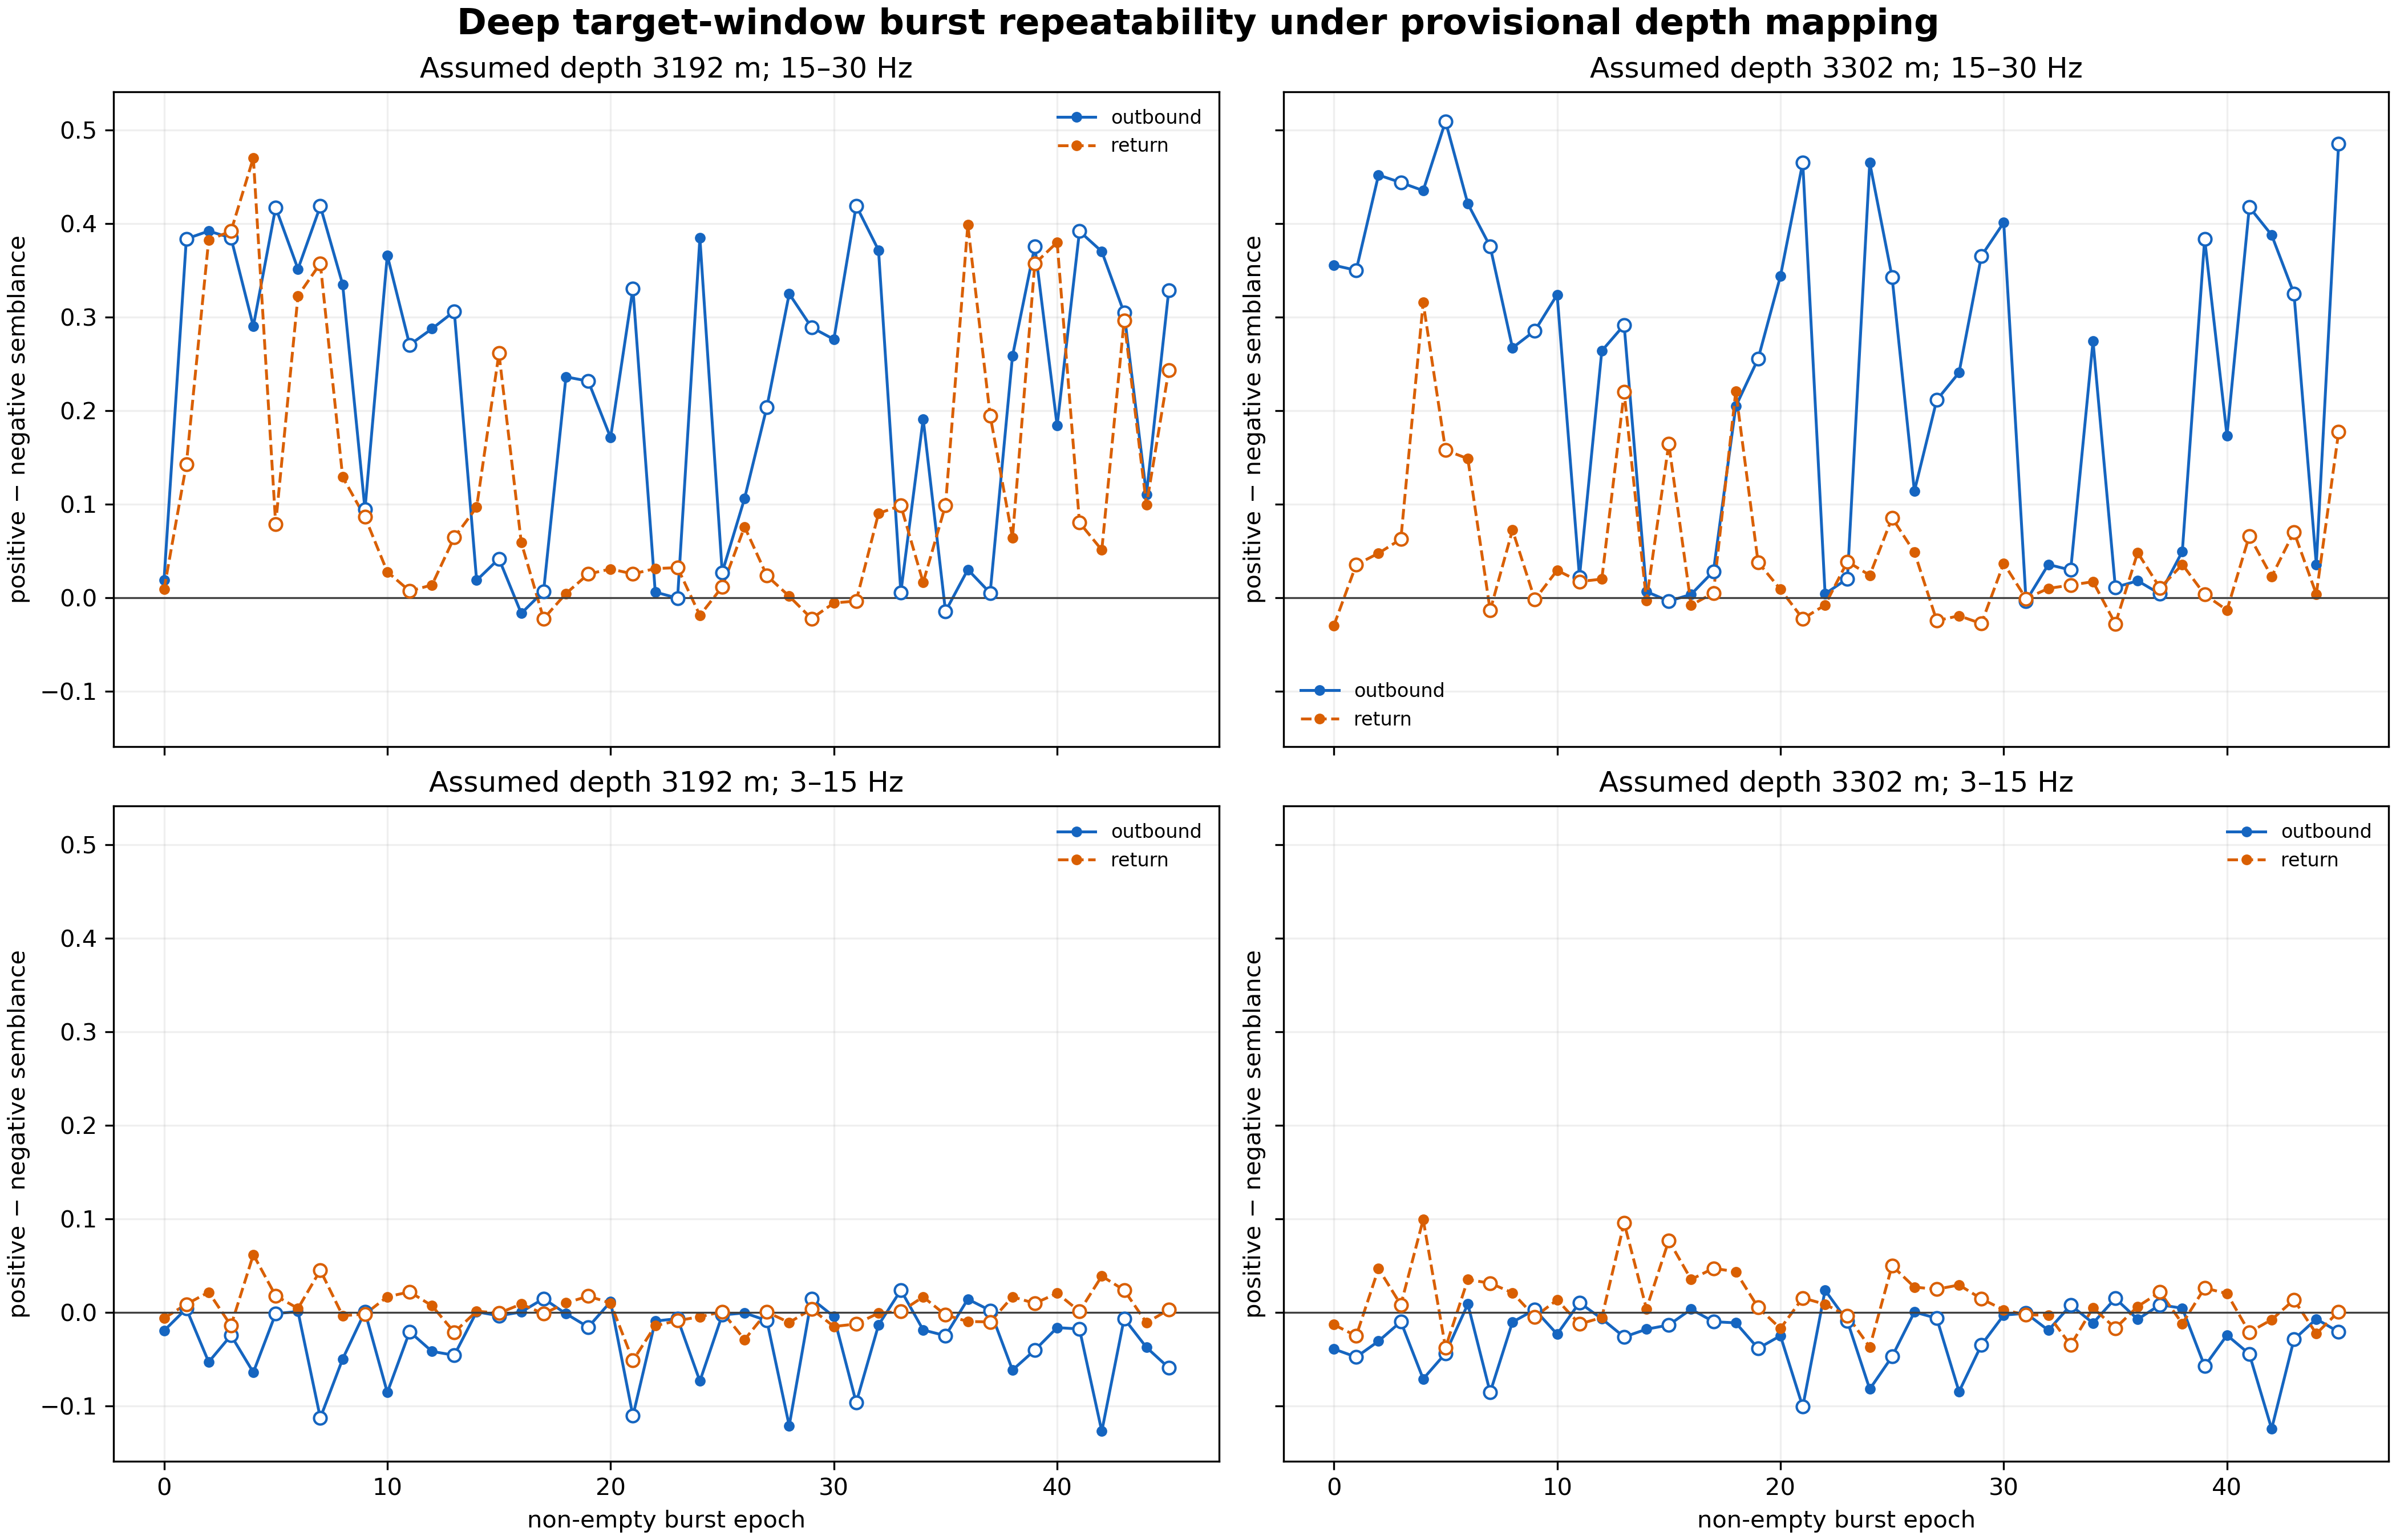
\includegraphics[width=0.98\linewidth]{deep_target_burst_repeatability.png}
\caption{\textbf{Held-out burst repeatability of the Deep target-window observable.} Each panel shows positive-minus-negative fixed-trajectory semblance for one assumed strand depth and frequency band; solid blue curves are outbound and dashed orange curves are reversed-return. Lines show all non-empty bursts; open markers overplot the 23 even-numbered validation bursts, while filled markers are the discovery points. The 15--30-Hz panels show positive directional coherence in 21/23 outbound and 20/23 return bursts at the assumed SDZ, and 21/23 outbound and 16/23 return bursts at the assumed CDZ. The 3--15-Hz panels are controls for the lower-frequency band. Control windows demonstrate that the mode is not confined uniquely to the provisional SDZ/CDZ interval. The statistic compares spatial ordering at a fixed trajectory selected from the independent discovery data; it is not an amplitude calibration, casing-displacement estimate, or creep-rate measurement. All depth labels inherit the conditional mapping $s_{\rm out}=\mathrm{depth}$ and $s_{\rm return}=3475.31-\mathrm{depth}$.}
\end{figure}

\takeaway{\preliminary: the positive 15--30-Hz Deep mode repeats across individual held-out bursts in the provisional target interval.  Because similar outbound coherence occurs in control windows, this establishes a repeatable baseline observable rather than a strand-specific deformation response.}

\section{Current evidence and limitations}

\begin{table}[H]
\centering
\small
\begin{tabular}{p{0.29\linewidth}p{0.16\linewidth}p{0.47\linewidth}}
\toprule
Statement & Status & Evidential basis \\
\midrule
AWD experiment reconstruction & \accepted & 49 qualifying bursts, 988 drops,
859 complete paired windows in 46 bursts \\
Nano coherent mode exists & \accepted & Visible ridge, moveout alignment,
spatial permutation $p=0.002$, weak pre-reference control \\
Nano direction and apparent speed & \accepted & Positive signed slowness;
approximately 2.95--2.99~km~s$^{-1}$ in the strongest band \\
Nano frequency dependence & \accepted as mode property & Burst bootstrap
resolves a positive slowness trend across the tested bands \\
Nano is direct P & Unresolved & Dispersion is compatible with guided/coupled
energy; absolute timing and geometry are incomplete \\
PGSI all-shot timing/moveout calibration & \preliminary & Five of six usable; canonical $t=i/200-0.200$~s; shot 1040 $2.982~[2.923,3.032]$~km~s$^{-1}$, only Nano match; others 5.20--5.47~km~s$^{-1}$ \\
Nano formation $V_P(z)$ & Not accepted & Requires a validated body-wave phase,
depth registration, source geometry, and synthetic resolution analysis \\
Deep slow spatial mode exists & \accepted & Odd/even replication, four fixed
validation permutation tests at $p=0.002$, positive sign in every burst \\
Deep slow mode is a tube wave & \preliminary & Speed and installation are
consistent, but fluid/casing model and independent wave-mode evidence are pending \\
Deep target-window observability & \preliminary conditional & Positive 15--30-Hz branch validates at assumed SDZ/CDZ depths on outbound and return legs; four explicit tests give $p=0.002$; depth mapping remains unverified \\
Source-history/compaction regression & Preliminary completed & 49 burst delays; cumulative-drop and signal-RMS proxies; no independent ground displacement \\
Nonmonotone delay component & Candidate, not tidal detection & Phase-free 24-hour harmonic: blocked-CV RMSE $0.297\to0.223$ ms; block-bootstrap $p=0.002$ \\
Fault opening/closing interpretation & Exploratory physical-phase test; unresolved & Sun/Moon degree-2 potential CCA: $r=0.366$; row $p=0.116$; three-burst block $p=0.263$; no traction sign \\
CCA tidal-timescale association & Exploratory / not confirmed & Phase-free $r=0.533$ (row $p=0.019$, block $p=0.118$); physical-phase $r=0.366$ (row $p=0.116$, block $p=0.263$); held-out correlations unstable \\
Deep conversion/fracture coordinate & Not supported & Five geometric branch
intersections; none passes the joint permutation threshold \\
Deep fiber-coordinate registration & Conditional / unresolved & HDF5 start-locus and hairpin coordinates audited; no surveyed depth origin or fiber-to-depth transform \\
Deep tube-wave forward consistency & Preliminary completed & All 24 validated candidates lie in the bounded 1.3--1.8-km-s$^{-1}$ fluid/compliance envelope; this is not phase identification \\
Borehole-log comparison & Not available & No transferred borehole logs were found; supplied $V_P/V_S$ arrays are formation-background context only \\
Current Nano monitoring limit & \accepted for estimator & 1\% is the smallest
tested two-direction 95\% correct-sign injection level for the selected
apparent-moveout estimator \\
Natural Parkfield-scale monitoring & Not supported at current design & Published
Parkfield changes are generally below the high-confidence AWD injection level;
this is a quantitative limitation, not a detected absence of fault response \\
\bottomrule
\end{tabular}
\caption{Evidence ladder for the current AWD analysis.  ``Accepted'' refers to
the stated empirical property only and must not be silently promoted to a more
specific phase or geological interpretation.}
\end{table}

\section{Recommended presentation sequence}

For an advisor meeting or poster draft, lead with the six core results in order:

\begin{enumerate}[leftmargin=*]
\item Core result 1: experiment and sampling geometry.
\item Core result 2: Nano signed frequency--slowness and dispersion.
\item Core result 3: drop-, burst-, and substack-scale repeatability.
\item Core result 4: installation-dependent Nano and Deep mode selection.
\item Core result 5: frequency aperture and apparent-moveout sensitivity.
\item Core result 6: PGSI timing/moveout calibration as a phase constraint.
\end{enumerate}

The full diagnostic figures that follow are supporting evidence, not additional
headline claims.  In particular, the PGSI all-shot diagnostic and the Deep
conversion-depth search should be shown only when the calibration limitations
are part of the discussion.

\section{Priority follow-up analyses}

\begin{enumerate}[leftmargin=*]
  \item \textbf{Interpret the all-shot PGSI separation.} Use the completed
  canonical timing convention, the 5/6 usability result, and the conditional
  1040--Nano registration to test whether the faster shots represent a different
  phase or coupling regime before any body-wave inversion.
  \item \textbf{Conditional Nano phase test.} Combine the registered PGSI result
  with frequency-dependent Nano trajectories, earliest-arrival ordering, the
  surveyed AWD source offset, and forward models for direct P and plausible
  guided modes. Attempt $V_P$ only if the body-wave interpretation survives.
  \item \textbf{Define and test change sensitivity.} Reconcile the null width,
  injection--recovery threshold, stack-scaling projection, and shallow burst
  scatter.  Run the 24-hour shallow sequence as a sinusoidal observability
  stress test with nuisance controls, phase-randomized nulls, and imposed
  0.5\%, 1\%, and 2\% changes.
  \item \textbf{Calibrated installation comparison.} Compare normalized
  coherence, bandwidth, spatial persistence, and repeatability now; compare
  absolute amplitudes only after gauge length, interrogator response, units, and
  coupling conventions are reconciled.
  \item \textbf{Deep physical interpretation.} The bounded fluid/compliance
  consistency test is complete.  Obtain the surveyed fiber-to-depth transform,
  deployment drawing, fluid/casing properties, and borehole logs, then replace
  the envelope with a real tube-wave dispersion model.  Because the
  branch-intersection test is negative, do not proceed directly to permeability
  inversion.
  \item \textbf{Physical-phase control (completed).} A low-precision UTC-phased
  Sun/Moon degree-2 potential was evaluated at all 49 bursts and compared with
  the source-corrected delay using row and three-burst block nulls plus blocked
  validation. It does not reproduce the phase-free candidate robustly; no
  opening/closing sign is assigned.
  \item \textbf{Next environmental/traction control.} Obtain an independent source
  settlement or compaction record, surveyed fault orientation, and local stress
  convention; then replace the scalar potential with a precision strain/traction
  predictor and repeat the held-out test.
  \item \textbf{Literature-constrained detectability statement.} After the
  estimator and empirical null are improved, compare the achieved $\Delta v/v$
  threshold with published Parkfield and SAFOD values, including the relevant
  frequency and depth kernels.  This is a detectability comparison, not an
  Earth-tide observation.
\end{enumerate}

\section{Analysis products}

\begin{center}
\small
\begin{tabular}{p{0.35\linewidth}p{0.56\linewidth}}
\toprule
Product & Generating analysis \\
\midrule
\path{source_time_audit.*} & \path{source_time_audit.py} \\
\path{record_section_inspection.png}, \path{null_tests.*} & \path{null_tests_and_inspection.py} \\
\path{mode_scan.*} & \path{analyze_modes.py} \\
\path{fk_dispersion.*} & \path{fk_dispersion.py} \\
\path{deep_sliding_fk.*} & \path{deep_sliding_fk.py} \\
\path{deep_tube_record_sections.png}, \path{deep_tube_repeatability.png},
\path{deep_tube_null_tests.png} & \path{deep_tube_validation.py} \\
\path{mode_repeatability.*} & \path{measure_repeatability.py} \\
\path{nano_frequency_observability.*} & \path{nano_frequency_observability.py} \\
\path{awd_multiscale_record_sections.*} & \path{multiscale_record_sections.py} \\
\path{nano_mode_identification.*} & \path{nano_mode_identification.py} \\
\path{deep_time_gated_branches.*} & \path{deep_time_gated_branches.py} \\
\path{nano_dvv_injection_recovery.*} & \path{nano_dvv_injection_recovery.py} \\
\path{core01--core06} & \path{core_figures_v7.py} \\
\path{pgsi_checkshot_allshots.*}, \path{pgsi_checkshot_registration.*} & \path{pgsi_checkshot_allshots.py} + \path{pgsi_reference/Check shots/} \\
\path{deep_registration_forward_model.*} & \path{deep_registration_forward_model.py}: HDF5 coordinate audit, hairpin registration, bounded fluid/compliance envelope, and explicit depth/log limitation \\
\path{deep_target_scan.*} & \path{deep_target_scan.py}: provisional 3000--3450-m target scan, signed branches, strand-depth validation, and channel-order nulls \\
\path{nano_tidal_compaction_regression.*} & \path{nano_tidal_compaction_regression.py}: source-history/coupling regression, blocked-CV test, and phase-free 24-hour delay harmonic stress test \\
\path{nano_tidal_cca.*} & \path{nano_tidal_cca.py}: CCA of phase-free tidal basis with source-corrected delay/coupling, row/block nulls, and blocked validation \\
\path{nano_physical_tide_cca.*}, \path{nano_physical_tide_predictors.csv} & \path{nano_physical_tide_cca.py}: UTC-phased low-precision Sun/Moon degree-2 potential, physical-phase CCA, row/block nulls, and blocked validation \\
\bottomrule
\end{tabular}
\end{center}


\section{Passive repeating-earthquake candidate catalog}

\figquestion{Can natural repeating earthquakes provide the longer-timescale
monitoring component that the 24-hour AWD experiment cannot provide by itself?}

The transferred Ellsworth catalog and original R geometry script have now been
translated into a reproducible Python event-screening branch.  The catalog
contains 329 events within 15~km of SAFOD from 1~May~2024 through
30~March~2026.  The event coordinates are shown in the same MH030-referenced,
45-degree rotated along-strike/depth and along-strike/time views used in the
original work.  A transparent screening layer ranks event pairs with horizontal
separation $\leq 1$~km, depth separation $\leq 1$~km, and magnitude difference
$\leq 0.5$.  These are event-selection gates, not a claim that the pairs are
physical repeaters.

The screen produces 6,325 candidate pairs; 6,112 are on distinct dates and at
least seven days apart.  The leading pairs are candidates for waveform
extraction, not detections.  A repeating-earthquake claim requires waveform or
coda correlation, focal-mechanism and location consistency, and confirmation
that both event times fall within continuous DAS coverage.

\begin{figure}[H]
\centering
\includegraphics[width=0.99\linewidth]{repeating/repeater_catalog_screen.png}
\caption{\textbf{Candidate repeating-earthquake sources for passive DAS
follow-up.} The left panel reproduces the catalog cross section using the MH030
reference point and the 45-degree rotation in the original script; symbol area
scales with catalog magnitude and color denotes event year.  The middle panel
shows along-strike coordinate versus UTC year, making spatially persistent
locations visible across multiple dates.  Red rings identify members of the
highest-ranked spatial candidates.  The right panel summarizes candidates under
explicit screening gates of $\leq1$~km horizontal separation, $\leq1$~km depth
separation, and $\leq0.5$ magnitude difference, with a modest preference for
separate dates and larger events.  The figure does not demonstrate repeating
waveforms, source equivalence, or a velocity change; those claims require
continuous DAS coverage at both origin times, waveform/coda cross-correlation,
location and mechanism checks, and uncertainty estimates.}}
\end{figure}

\takeaway{The catalog branch is complete as event selection but conditional as
DAS monitoring.  The June~2026 AWD records do not overlap the catalog, so no
passive correlation or creep-related velocity change is reported here.  The
next required input is continuous DAS data covering the candidate timestamps;
the active-source AWD result will then provide the calibrated processing and
installation baseline.}

\section{Continuous-DAS coverage audit for repeater candidates}

\figquestion{Which catalog candidates can actually be tested with the continuous
DAS archive used by the ambient-noise analyses?}

The ambient-noise archive is indexed by
\path{/oak/stanford/groups/ettore88/data/SAFOD/SAFODAS1-harddrive-transfer/SAFOD_2024_2025.csv}.
It contains 392,095 short HDF5 file records, of which 392,079 have valid
start/end intervals.  Joining catalog origin times to those intervals gives
exact coverage for 146 of 329 catalog events and for 1,200 candidate pairs at
both event times.  The remaining 183 events are outside the available archive,
primarily in the later portion of the catalog.

\takeaway{This is an input audit, not a waveform result.  A covered interval
may still be unreadable, have insufficient signal-to-noise ratio, or require a
wider extraction window because of origin-time uncertainty.  The next analysis
is restricted to covered pairs and will extract event-centered Nano/Deep windows
before computing waveform and coda correlation.}

\section{Covered-pair waveform pilot}

\figquestion{Do catalog-selected, spatially close earthquake pairs produce
repeatable DAS waveforms when exact event-containing HDF5 segments are
available?}

The ten highest-ranked pairs with coverage at both event times were tested with
a memory-safe extractor.  For each event, the full 60-s segment was scanned in
100-channel batches to estimate a 5--50~Hz energy arrival.  A padded 6-s window
was then filtered and normalized using all 900 channels, and channel-wise
normalized maximum correlation was evaluated over $\pm0.5$~s after arrival
alignment.

Seven of the ten pairs produced usable windows at both events.  Their median
channel-wise maximum correlations range from 0.139 to 0.177, and no pair has
more than 0\% of channels above 0.5 correlation.  This pilot does not confirm
repeating earthquakes.  It does establish that catalog proximity alone does not
guarantee a repeatable DAS waveform.

\takeaway{This is a preliminary triage result, not a final negative conclusion
about passive monitoring.  Non-identical sources, catalog-origin uncertainty,
event signal-to-noise ratio, installation changes, and imperfect phase/window
selection remain possible explanations.  Event-specific phase quality control,
matched non-candidate controls, and a targeted coda-window test are required
before abandoning or promoting the repeater branch.}

\section{Summary}

The analysis supports more than ``there is energy in the data.''  It supports a
statistically significant, repeatable, positive-slowness Nano mode, a
frequency-dependent monitoring aperture, a distinct and independently validated
slow Deep mode, and an empirical sensitivity estimate for the accepted Nano
apparent-moveout observable.  The present configuration should not be presented
as resolving typical natural Parkfield-scale $dv/v$ changes.  The next scientific
branch is instead to (1) use the completed PGSI calibration and forward models
to discriminate direct-P from guided/coupled explanations, (2) obtain the missing Deep fiber-to-depth registration and logs for a
true tube-wave model, and (3) refine the change-sensitivity stress test.  The
current bounded forward test supports tube-wave-like kinematics only.  The source-history delay regression adds a candidate nonmonotone 24-hour component. Phase-free CCA does not confirm it under serially aware nulls, and the UTC-phased Sun/Moon potential control is weaker (r=0.366; block p=0.263) and does not support a tidal opening/closing interpretation.  A formation-$V_P$ or
permeability inversion remains conditional on those checks.  The completed
Deep branch search is itself informative: it validates a slow directed mode
but finds no statistically supported conversion coordinate.


\subsection{Ambient-noise interferometry replication audit}
The earlier ambient-noise analysis was an extensive five-month reproduction attempt, not an untried branch. The saved implementation differs from Lellouch et al. (2019) in acquisition, virtual-source geometry, stacking design, spatial sampling, and correlation scaling. It correlated channel 200 with all channels in a 150--800 subset, used selected short files rather than matched complete one-day stacks, hard-coded 1-m spacing despite the archive metadata, and retained an unnormalized FFT correlation whose saved values exceed unity. The current archive also differs from the released 2017 data used in the paper (900 channels and 2024--2025 metadata versus 800 channels and 250-Hz sampling). The resulting near-zero-lag source autocorrelation is therefore a valid result for that branch but not a controlled negative replication. A fair follow-up must implement both published geometries, resolve every file path, compare normalized and phase-only correlations, stack complete UTC days, and use seven-day uncertainty and receiver-position permutation nulls. The project record labels the earlier result an inconclusive reproduction attempt.


\subsection{Controlled Lellouch-style ambient interferometry transfer test}
A memory-safe implementation was run on three independent 10-file chunks (30 segments, approximately 30 minutes) from the 2024--2025 archive. It used the published top-channel and 50-m source--receiver geometries, 5--20~Hz filtering, 5-s running-absolute-mean normalization, the measured 1.020952-m spacing, and pairwise RMS-normalized correlations. The combined score at 3.2~km~s$^{-1}$ was $-0.00266$; the weak maximum was $0.00388$ near 1.65~km~s$^{-1}$. A receiver-position permutation null gave $p=0.875$. This is a negative transfer pilot, not a rejection of the 2017 Lellouch result, because the archive and duration differ. The next test is a complete-day chunked stack.


\subsection{Duration-matched baseline and F--K extension}
Seven independent 10-file chunks (70 segments, approximately 70 minutes) were combined with the published top-channel and 50-m geometries. The 3.2~km~s$^{-1}$ score was $-0.00321$, the weak maximum was $0.00481$ near 1.40~km~s$^{-1}$, and a receiver-position permutation null gave $p=0.561$. The result is a stronger negative transfer baseline but remains shorter than a complete day. F--K filtering is treated as a secondary, non-circular extension: a fixed 5--20~Hz, 2.5--4.5~km~s$^{-1}$ signed-wavenumber wedge will be applied before recomputing the same correlations, with complementary-wedge and held-out controls.


\subsection{Exploratory F--K-filtered ambient correlations}
A fixed positive signed-wavenumber wedge retaining 5--20~Hz and apparent velocities from 2.5--4.5~km~s$^{-1}$ was applied before recomputing the top-source correlations. The 10-segment test gives a score of 0.01257 at 3.2~km~s$^{-1}$ and a maximum of 0.03141 near 3.78~km~s$^{-1}$. This is exploratory because the mask retains the target velocity interval by construction. Negative-wavenumber, two-sided, equal-bandwidth complementary, receiver-permutation, and held-out controls are required before interpreting the enhancement.


\subsection{Signed F--K control result}
The positive signed wedge gives a 3.2~km~s$^{-1}$ score of 0.0126 with permutation $p=0.996$, whereas the negative signed wedge gives a peak at 3.075~km~s$^{-1}$, score 0.2846 at 3.2~km~s$^{-1}$, and $p=0.002$ in ten segments. The two-sided wedge also enhances the mode (score 0.1197, $p=0.002$), while an equal-width complementary wedge does not (score $-0.1156$, $p=0.778$). Combining three independent chunks yields peak 3.075~km~s$^{-1}$, score 0.2952, and $p=0.0005$. This is a preliminary F--K-selected recovery: the fixed wedge contains the target velocity interval, so held-out days and wedge-sensitivity tests are required before calling it a Lellouch reproduction.


\subsection{Segment-duration clarification}
For this archive, one HDF5 segment contains 30,000 samples at the 500-Hz output rate, or 60~s. Consequently, 10 segments represent approximately 10~min, 30 segments approximately 30~min, and 70 segments approximately 70~min. This corrects the elapsed-time labels in earlier descriptions; it does not change any correlation, moveout, or null result.


\subsection{Longer signed F--K stack}
The frozen negative signed-wavenumber wedge was extended to seven independent 10-file chunks (70 segments, approximately 70~min). The aggregate peak is 3.075~km~s$^{-1}$, the score at 3.2~km~s$^{-1}$ is 0.2947, and a 5,000-permutation receiver null gives $p=0.0002$. All seven chunk scores are positive. This is a stable 70-minute F--K-selected observable, but not yet a complete-day reproduction or an independent velocity estimate because the wedge contains the target interval. The complete-day and seasonal products are now available below; held-out-day and nearby-wedge tests remain the appropriate robustness checks.


\subsection{Seasonal robustness of the ambient F--K result (running)}
\figquestion{Is the approximately 3.2~km~s$^{-1}$ signed branch persistent across the 14-month archive, or is the February baseline day atypical because of season, coupling, weather, or local seismicity?}

This test was initiated because a single complete-day stack cannot establish that the observed wavefield is representative of the archive. Two complete days were selected from each meteorological season using a fixed random seed. A day was admitted only if its index contained at least 1,400 one-minute files and no inter-file gap greater than 65~s. The selected dates are:

\begin{center}
\begin{tabular}{lll}
\toprule
Season & Date 1 & Date 2 \\
\midrule
DJF & 2024-12-20 & 2025-02-24 \\
MAM & 2024-05-11 & 2025-03-04 \\
JJA & 2024-06-17 & 2024-06-26 \\
SON & 2024-10-28 & 2024-11-30 \\
\bottomrule
\end{tabular}
\end{center}

Each day is processed independently with the same 5--20~Hz bandpass, 5-s running-absolute-mean temporal normalization, and negative, positive, and two-sided signed F--K branches. Earthquake-containing intervals are retained; temporal normalization suppresses their amplitude leverage but does not remove their waveforms. Day-level products are aggregated only after the individual-day stacks and permutation nulls are complete. The comparison will report peak apparent velocity, normalized coherence at 3.2~km~s$^{-1}$, signed-branch asymmetry, and the fixed-passband response. The negative and positive branches are evaluated separately so that a seasonal change in polarity or coupling is not hidden by a two-sided stack.

At the time of this guide revision, the processing is still running. The status is therefore \planned, and no seasonal persistence claim is made. The live notebook section records completion fraction and will display the day-level and across-day products once the aggregation file exists. A consistent peak velocity and branch asymmetry across seasons would support a persistent propagating wavefield; systematic seasonal changes would instead identify environmental or coupling dependence that must be included in the interpretation.

\takeaway{Seasonal validation is a robustness test, not an additional significance claim. It determines whether the February result can be treated as an archive-wide property.}


\subsection{Independent unfiltered verification (running)}
\figquestion{Is the weak unfiltered transfer result caused by the data, or by an implementation difference?}

The seasonal F--K run alone cannot distinguish a physical observability effect from a software or downsampling artifact. An independent control is therefore being run through the exact-resolution path in \code{ambient\_transfer\_test.py}. This path is separate from the F--K implementation: it reads the full-resolution traces, uses the published top-channel and 50-m source--receiver geometries, measured spatial spacing, 5--20~Hz filtering, 5-s running-absolute-mean temporal normalization, and RMS-normalized correlations. The selected days and completeness criteria are identical to the seasonal F--K test. Earthquake-containing intervals remain in the records and are not catalog-muted.

The verification is intentionally resumable and produces day-level products before any across-day aggregate. Agreement between this independent full-resolution path and the F--K routine's unfiltered control would argue against an implementation bug. A strong F--K branch alongside a weak independently verified unfiltered result would instead indicate that F--K isolation materially changes observability. Until the unfiltered day-level products and permutation nulls exist, no conclusion is assigned to this branch.

\takeaway{The F--K result is not being used to excuse a possible unfiltered coding error; the exact-resolution unfiltered path is being rerun as an independent check.}


\subsection{Axis convention for the Lellouch comparison}
Lellouch et al. organize the top-source geometry by receiver position along the fiber, treated approximately as depth, and the constant-offset geometry by pair midpoint along the fiber. The revised transfer figure follows those physical coordinates rather than using the ambiguous labels ``separation'' and ``pair index.'' For the top-source geometry, receiver position relative to the top virtual source is numerically equal to source--receiver separation because the source is channel 0. These remain fiber coordinates, not independently registered measured depths.

\takeaway{The axis change is a plotting convention, not a change to the correlations or moveout calculation. It makes the comparison with Figure 7 of Lellouch et al. explicit while preserving the distinction between fiber coordinate and borehole depth.}


\subsection{Interim five-hour unfiltered versus F--K comparison}
\figquestion{Does the F--K enhancement appear before the full seasonal stack, and is the corresponding unfiltered control independently weak?}

The first selected winter day (2024-12-20) has enough completed checkpoint products for a five-hour interim stack using 300 one-minute files. The exact-resolution unfiltered path gives a normalized-correlation score of 0.0003 at 3.2~km~s$^{-1}$, below its receiver-permutation 95th-percentile maximum (p = 0.265). The negative signed F--K branch peaks at 3.075~km~s$^{-1}$, has score 0.266 at 3.2~km~s$^{-1}$, and gives p = 0.0005; the positive branch is not significant, while the two-sided branch remains enhanced.

All traces were detrended, filtered from 5--20~Hz, and normalized by a 5-s running absolute mean. Earthquake-containing intervals were retained. Because the F--K wedge was selected to include 2.5--4.5~km~s$^{-1}$, its null result is conditional on that selection and is not an independent velocity estimate. This is an interim one-day diagnostic; the completed seasonal aggregate is reported below.

\takeaway{The early checkpoint evidence supports the working hypothesis that signed F--K isolation materially improves observability, while the exact-resolution unfiltered control remains weak.}


\subsection{Figure: five-hour unfiltered versus F--K comparison}
\figquestion{Does the F--K enhancement appear in an interim stack, while the independently implemented unfiltered control remains weak?}

\begin{figure}[H]
\centering
\includegraphics[width=0.98\linewidth]{ambient_transfer/interim_2024-12-20_n300.png}
\caption{\textbf{Five-hour interim ambient transfer test from 2024-12-20.} (a) Exact-resolution unfiltered Lellouch-style top-source correlations with 2.5, 3.2, and 4.0~km~s$^{-1}$ reference moveout lines; (b) the same geometry after the negative signed F--K wedge with the same reference lines; (c) trial-velocity scores for unfiltered, negative, positive, and two-sided branches; and (d) scores at 3.2~km~s$^{-1}$ with receiver-permutation 95th-percentile thresholds. The unfiltered score at 3.2~km~s$^{-1}$ is 0.0003 (p = 0.265), whereas the negative branch reaches 0.266 (p = 0.0005). All records were detrended, filtered from 5--20~Hz, and temporally normalized by a 5-s running absolute mean; earthquake-containing intervals were retained. The F--K wedge includes the target velocity range by construction, so its significance is conditional and does not constitute an independent velocity estimate. This is a preliminary one-day partial stack; the completed seasonal aggregate is reported in the v41 section below.}
\end{figure}


\subsection{Lellouch Figure 7c-style receiver-by-receiver correlation section}
\figquestion{Does the apparent arrival form a continuous receiver-position--lag packet, rather than appearing only as isolated high correlation values?}

\begin{figure}[H]
\centering
\includegraphics[width=0.98\linewidth]{ambient_transfer/interim_2024-12-20_n300_lellouch7c.png}
\caption{\textbf{Receiver-by-receiver correlation section for the five-hour interim stack.} Each row is a top-source cross-correlation at one receiver position along the fiber; rows are normalized independently for display. The dashed line is the 3.2~km~s$^{-1}$ reference moveout. The left panel is exact-resolution unfiltered and the right panel is negative signed F--K isolated. This is analogous to the receiver-position section in Figure 7c of Lellouch et al. (2019), but uses a five-hour interim stack rather than a one-day stack.}
\end{figure}


\subsection{Original Lellouch Figure 7c reference}
The file \code{l7c.png}, copied from the supplied Lellouch output directory, is embedded in the notebook as a reference image immediately before the analogous five-hour current-data section. It is not a result from the 2024--2025 SAFOD archive. Its purpose is to make the receiver-position--lag presentation and moveout-line convention explicit.


\subsection{Direct Lellouch-style black-and-white wiggle plots}
The color receiver-position sections are retained as diagnostic products. Additional black-and-white wiggle figures show the same five-hour unfiltered and negative F--K correlations using independently normalized traces, receiver-position vertical offsets, and a 3.2~km~s$^{-1}$ reference moveout. These figures are intended for direct visual comparison with the supplied Lellouch 7c reference and do not replace the quantitative color products.


\subsection{Preliminary apparent-velocity scan of the negative F--K ridge}
\figquestion{Does the current-data ridge support the published 3.2~km~s$^{-1}$ reference as a single moveout, or does a different apparent velocity or a curved moveout describe it better?}

The five-hour negative-branch section was examined by taking the maximum-correlation lag in each receiver-position row. The first approximately 350--400~m follows an apparent moveout of about 3.1--3.2~km~s$^{-1}$. At larger offsets the ridge bends to later lags, corresponding to a slower apparent moveout of approximately 2.4--2.7~km~s$^{-1}$. An intercept-aware robust fit over 50--650~m gives 2.64~km~s$^{-1}$, with an intercept of about -20~ms; the best constant-velocity scan is approximately 2.65~km~s$^{-1}$. These numbers summarize the selected ridge and should not be interpreted as an absolute formation $V_P$.

The mismatch with 3.2~km~s$^{-1}$ is therefore not evidence by itself that the published result is wrong. The datasets differ in deployment, interrogator bandwidth, gauge length, source/receiver geometry, and stacking interval. In addition, the present plot is F--K selected over a prescribed velocity wedge, and row maxima are quantized at the correlation lag sample interval. The bend could reflect dispersion, mixed arrivals, finite-aperture effects, or a ridge-picking/aliasing artifact. The next test is to repeat the velocity scan across the independent seasonal days and frequency bands, then evaluate held-out data with a mask chosen from separate records.

\begin{figure}[H]
\centering
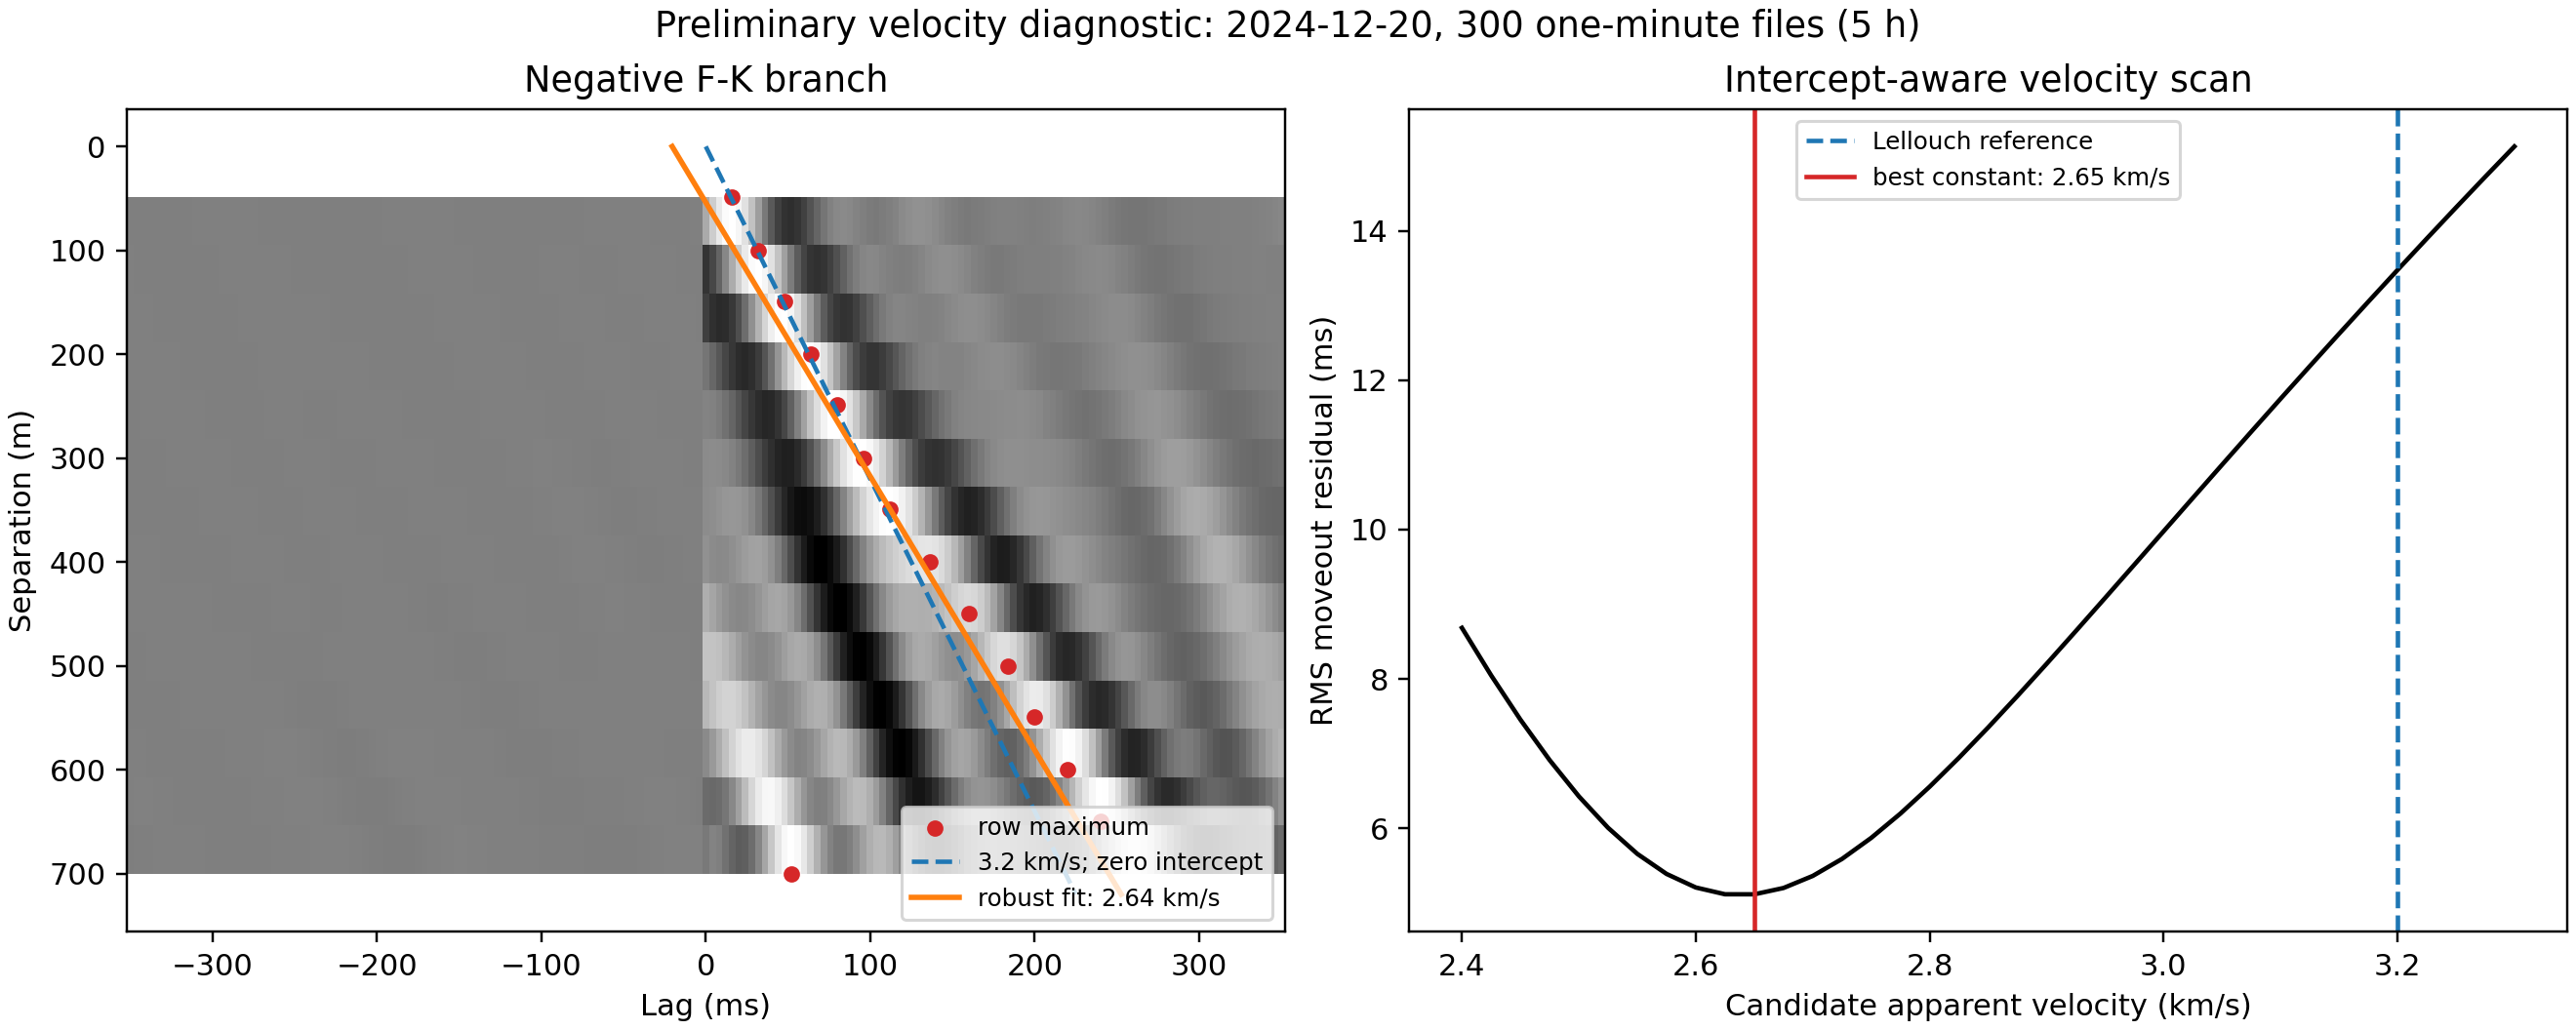
\includegraphics[width=0.98\linewidth]{fk_velocity_moveout_diagnostic.png}
\caption{\textbf{Preliminary apparent-velocity diagnostic for the five-hour negative signed F--K stack on 2024-12-20.} Left: receiver-position correlation section with the row-maximum ridge (red), the zero-intercept 3.2~km~s$^{-1}$ reference used for the Lellouch comparison (blue dashed), and the intercept-aware robust fit over 50--650~m (black). Right: RMS residual of the row-maximum moveout for candidate constant velocities after optimizing the intercept. The first 350--400~m is close to 3.1--3.2~km~s$^{-1}$, whereas the longer-offset ridge is slower; the resulting 2.64--2.65~km~s$^{-1}$ constant-fit value is descriptive, F--K conditional, and not an absolute formation-velocity estimate. The 700-m row is displayed but excluded from the fit because its lag maximum jumps to an isolated edge-like value.}
\end{figure}


\subsection{Inherited depth convention from the same cemented main-hole fiber}
The current ambient-data records use the same physical cemented SAFOD main-hole fiber analyzed by Lellouch et al. The cemented installation makes post-installation movement of the fiber origin negligible. We therefore adopt Lellouch's approximate convention that along-fiber receiver position tracks measured well depth, subject to the smaller remaining uncertainties in channel origin, spatial calibration, excess fiber length, and measured-depth versus vertical-depth convention. This changes the registration status from ``unavailable'' to ``conditionally inherited from the documented same-fiber installation.''

The immediate comparison is between the current negative F--K ridge curvature and the approximately 500--520~m velocity-ratio/mode-conversion anomaly reported by Lellouch et al. The comparison is still a hypothesis test: current channel zero must be tied to the same physical fiber position used in the 2017 analysis, and the current row coordinate must be converted using the measured channel spacing. A stable feature at the same registered coordinate across independent days and frequency bands would support a common subsurface cause; a frequency-dependent or non-reproducible feature would favor dispersion or mixed-mode processing effects.


\subsection{Conditional test of the 500--520~m Lellouch anomaly}
\figquestion{Under the inherited same-fiber depth convention, does the AWD F--K moveout change localize to the previously reported 500--520~m SAFOD anomaly?}

We treated current channel 0 and the measured 1.020952-m channel spacing as inherited from the same cemented main-hole fiber used by Lellouch et al. and analyzed 369 available ten-minute negative-branch F--K products from four dates. For each product, the maximum-correlation lag in each receiver-position row was picked. The early 50--350~m segment has date-level median apparent velocities of 3.13--3.19~km~s$^{-1}$, while the late 450--650~m segment has medians of 2.49--2.61~km~s$^{-1}$. Thus the curvature is repeatable across dates under the assumed registration. A descriptive two-segment breakpoint scan gives date-level medians of 350--425~m, with broad intervals extending to approximately 450~m; it does not uniquely localize the change at 500--520~m.

The result supports a repeatable transition-like feature in the current wavefield and makes the Lellouch anomaly a legitimate comparison target, but it does not establish that the two features are identical. The mismatch may reflect the broadness of the transition, fiber-coordinate uncertainty, dispersive or mixed-mode moveout, or the fact that row maxima are quantized at the lag sample interval. The completed frequency-band and seasonal products now provide that comparison. They support a broad transition-like feature, but the registered coordinate remains conditional and does not uniquely identify the Lellouch anomaly or a lithologic boundary.

\begin{figure}[H]
\centering
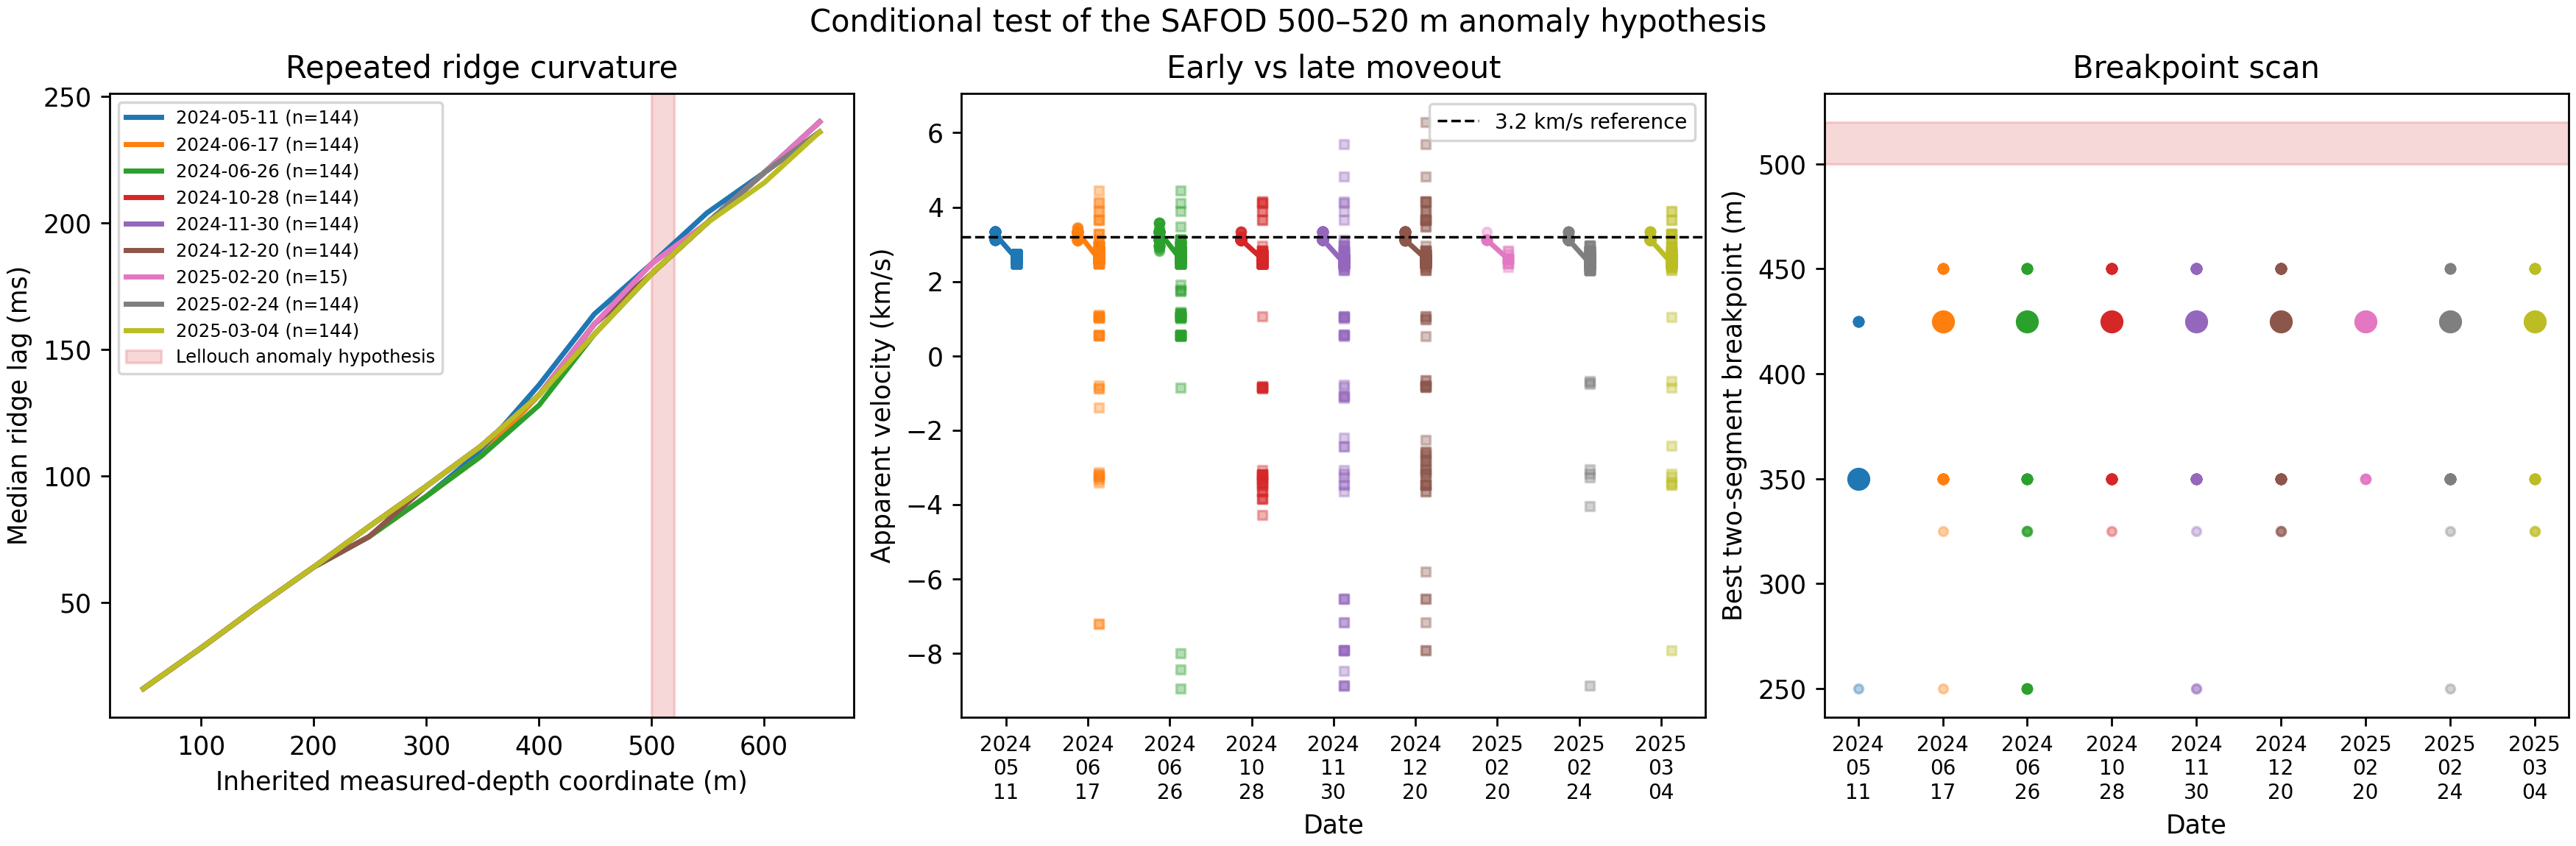
\includegraphics[width=0.98\linewidth]{fk_geology_anomaly_test.png}
\caption{\textbf{Conditional same-fiber test of the SAFOD 500--520~m anomaly hypothesis.} Negative signed F--K row-maximum moveout was measured in 369 ten-minute products from four dates, under the assumption that current channel 0 and 1.020952-m spacing inherit Lellouch's approximate fiber-position-as-depth convention. Left: date-level median ridge lags; the shaded interval marks 500--520~m. Middle: early (50--350~m) and late (450--650~m) robust apparent velocities for each product, with date medians connected. Right: descriptive two-segment breakpoint estimates. Early velocities cluster near 3.13--3.19~km~s$^{-1}$ and late velocities near 2.49--2.61~km~s$^{-1}$, demonstrating repeatable curvature. Breakpoints center at 350--425~m rather than uniquely at 500--520~m, so the result supports a transition-like wavefield feature but does not identify the Lellouch anomaly or a lithologic boundary. Ten-minute products are not independent observations; date-level summaries and independent frequency-band tests are required for confirmation.}
\end{figure}


\subsection{Ambient-noise virtual source, F--K processing, and departure from Lellouch et al.}
\figquestion{What exactly is the ambient-noise observable, where is its virtual source, and why does the corrected branch differ from the earlier unsuccessful reproduction?}

\paragraph{Virtual source and axes.} The top-source geometry uses DAS channel 0 as a fixed reference trace: it is a \emph{mathematical virtual source} created by cross-correlation, not a physical source at the wellhead. The reference is correlated with receivers at approximately 50, 100, ..., 700~m along the fiber using the measured current spacing $d x=1.020952$~m. Thus receiver position relative to channel 0 is the displayed along-fiber coordinate. The second geometry uses fixed approximately 50-m source--receiver separation, with pair midpoint as the vertical coordinate. Neither axis is independently re-registered within this ambient branch.

\paragraph{Current processing.} Each 60-s record is detrended, bandpass filtered from 5--20~Hz, and divided by a 5-s running mean of absolute amplitude. Earthquake-containing intervals remain in the records; temporal normalization suppresses their amplitude leverage but does not remove their waveforms. Correlations are pairwise RMS-normalized. For the F--K extension, the normalized traces are decimated by two, transformed with a two-dimensional FFT, and multiplied by a signed velocity wedge. The primary negative branch retains 5--20~Hz energy with apparent velocity 2.5--4.5~km~s$^{-1}$ and $f k<0$; positive and two-sided branches, an equal-band complement, receiver permutations, and unfiltered controls are evaluated separately. The wedge includes the target velocity interval by construction, so its significance is conditional on that processing selection.

\paragraph{What differs from Lellouch et al. (2019).} The current archive is a later acquisition and is not the original 2017 continuous record. The earlier unsuccessful branch used channel 200 as the reference, hard-coded 1-m spacing, selected short files rather than a complete UTC day, and used unnormalized FFT correlations. The corrected transfer branch uses the published top-channel and fixed-50-m geometries, measured spacing, 5-s temporal normalization, pairwise RMS normalization, and complete-day/chunked stacking. F--K isolation is an additional processing experiment, not a step in the published Lellouch ambient-interferometry method.

\paragraph{Why the signal appears now.} The present recovery cannot yet be attributed to one change alone. The strongest methodological changes are removal of the channel-200 geometry error, correct spatial calibration, bounded correlation normalization, more coherent stacking, and signed F--K isolation of a directional branch. The current result should therefore be described as a successful \emph{transfer test on a different acquisition}, not an exact reproduction of the 2017 paper. The completed seasonal and frequency-band controls show that the F--K enhancement persists across dates, while the apparent transition is sensitive to passband and row-maximum stability.

\takeaway{The advisor-facing short version is: channel 0 is the fixed virtual source; the current corrected branch matches Lellouch's geometry and normalization much more closely, while F--K isolation is our added extension. The earlier failure was not a controlled reproduction because its geometry, stacking, acquisition, and correlation scaling differed.}


\subsection{Synthetic signed F--K convention check and relation to Lellouch filtering}
\figquestion{Does the sign of $F K$ in the current implementation select the expected coordinate-propagation direction, and where did Lellouch et al. use F--K filtering?}

A synthetic wave $u(z,t)=\cos[2\pi f(t-z/v)]$ was passed through the same decimation and signed F--K masks as the ambient branch, using $f=10$~Hz and $v=3.2$~km~s$^{-1}$. This wave propagates toward increasing fiber coordinate $z$ and was retained by the $F K<0$ branch (output RMS 0.560 versus 0.057 for $F K>0$). The opposite wave $\cos[2\pi f(t+z/v)]$ propagates toward decreasing $z$ and was retained by $F K>0$ (output RMS 0.560 versus 0.056 for $F K<0$). The synthetic confirms the code's coordinate-direction sign. It does not by itself label either branch physically as upgoing or downgoing; that requires the fiber orientation, depth direction, and correlation time convention.

Lellouch et al. do explicitly use F--K filtering, but in their earthquake S-wave processing (their Figure 5), after P-moveout correction. Their filter retains upgoing events below 11~km~s$^{-1}$ and 10--80~Hz energy to suppress P events and downgoing free-surface reflections before S-wave picking. Their ambient-field interferometry section instead describes 5--20~Hz bandpass-filtered cross-correlations, causal/anti-causal comparison, and 1-day stacks; it does not describe the signed 2.5--4.5~km~s$^{-1}$ F--K wedge used in this project. The current ambient F--K operation is therefore an added transfer-test extension, not a hidden step copied from their ambient method.

\begin{figure}[H]
\centering
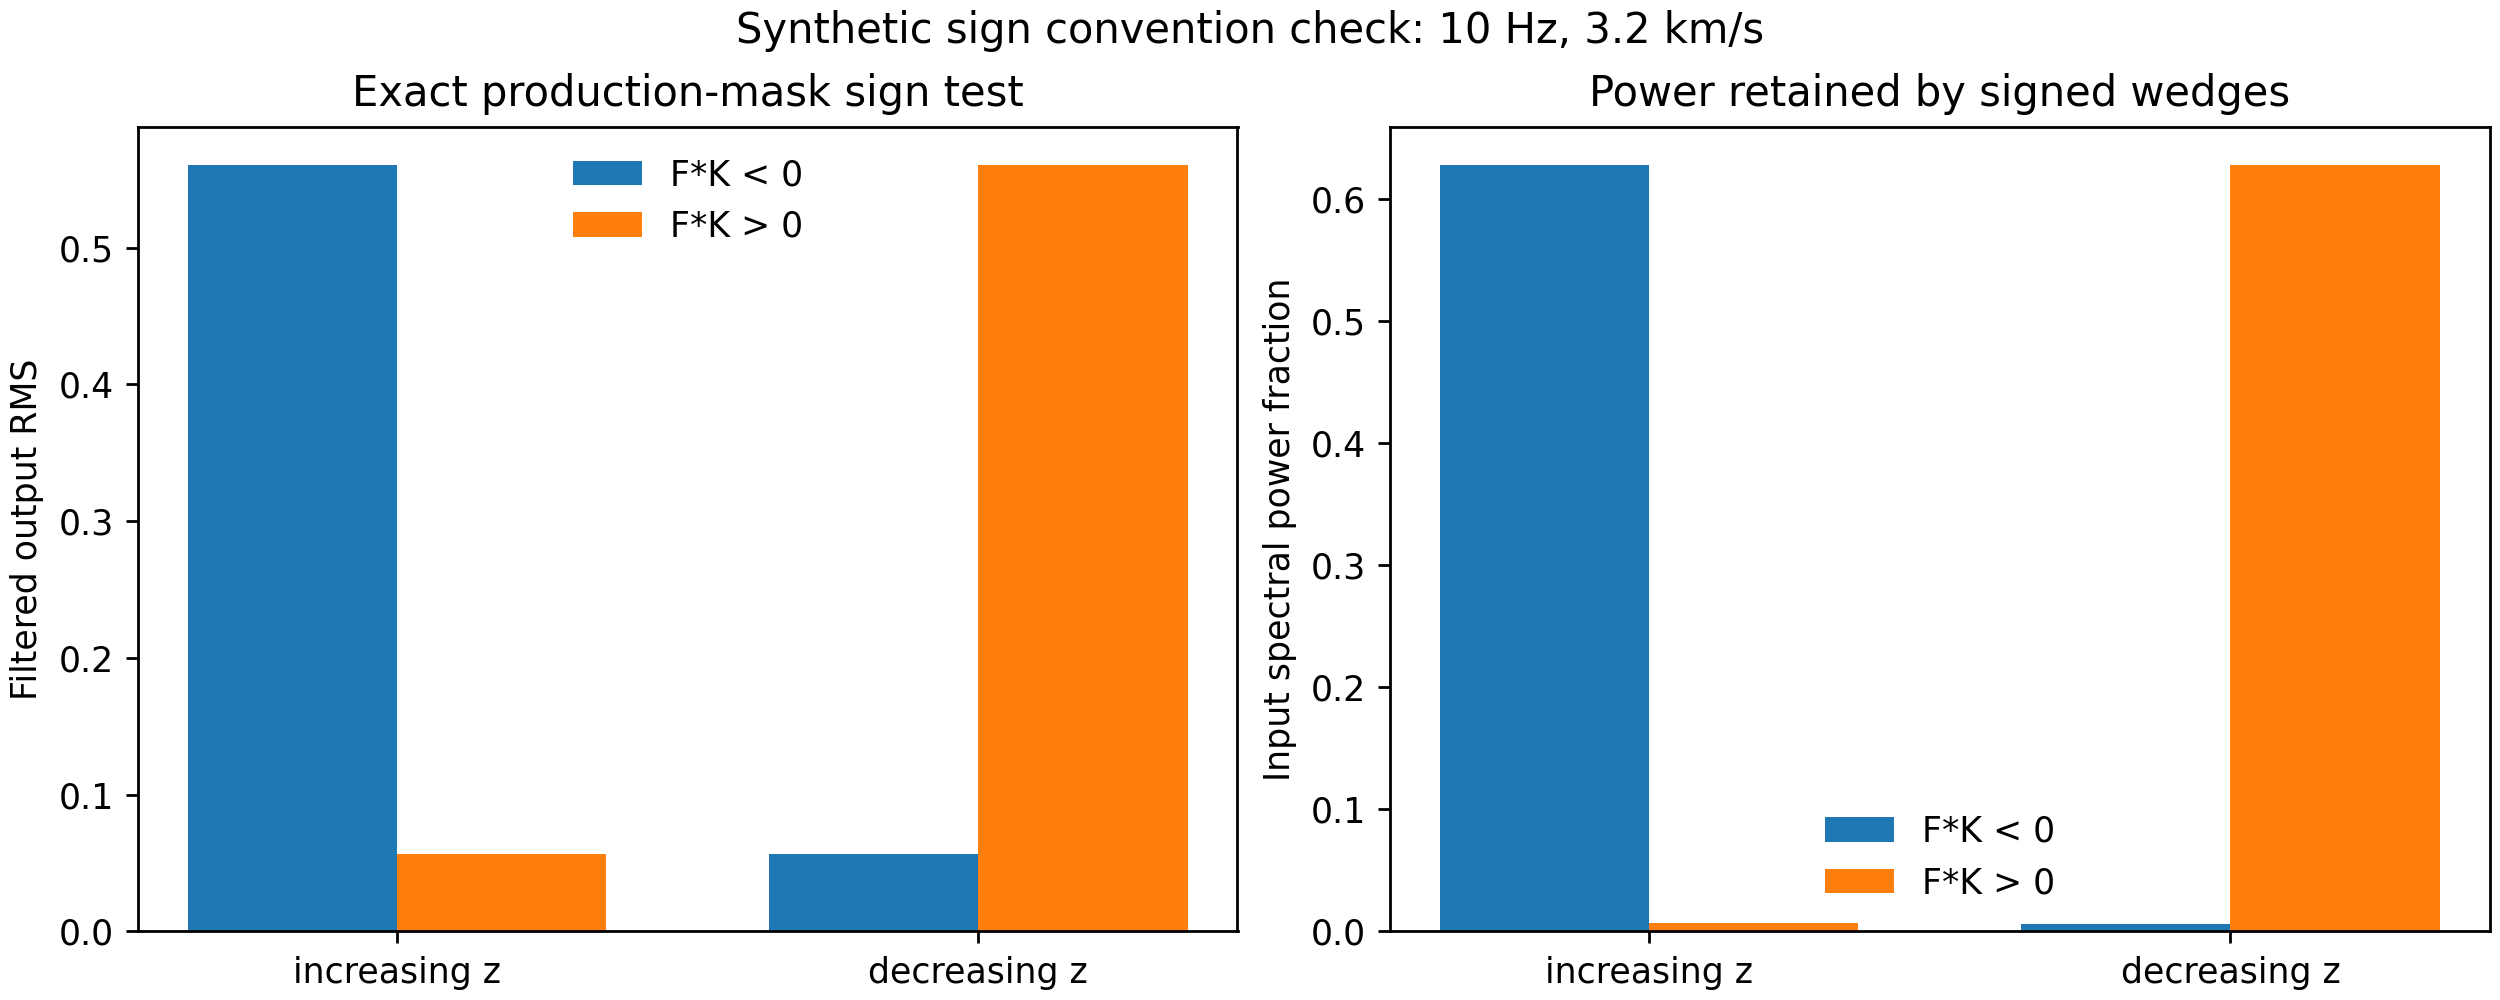
\includegraphics[width=0.78\linewidth]{fk_sign_synthetic_test.png}
\caption{\textbf{Synthetic sign convention check for the ambient signed F--K masks.} A 10-Hz, 3.2-km-s$^{-1}$ wave traveling toward increasing fiber coordinate is retained by $F K<0$, whereas the opposite coordinate-propagating wave is retained by $F K>0$. The test uses the production code's 2-fold spatial/temporal decimation and 5--20~Hz, 2.5--4.5~km~s$^{-1}$ wedge. The result validates coordinate-direction selection only; physical upgoing/downgoing labels require independent fiber orientation and time/depth registration.}
\end{figure}


\subsection{Physical interpretation of the Nano signed F--K branches}
For the Nano ambient branch, the coordinate-direction labels can be converted to physical propagation labels under the documented geometry. Channel 0 is the shallow/top end of the same cemented main-hole fiber, increasing Nano channel coordinate follows the fiber downhole, and the time axis increases forward. The active-source records independently show arrivals at progressively later times at increasing Nano coordinate. Combined with the synthetic sign check, this gives $F K<0$ as the downgoing surface-to-depth branch and $F K>0$ as the upgoing depth-to-surface branch for Nano.

This physical label is specific to the Nano top-source geometry and its stated coordinate convention. It should not be transferred automatically to the Deep hairpin, whose outbound/return orientation is still represented with explicit coordinate reversals and whose physical depth direction remains conditional.

\takeaway{For Nano, the negative signed F--K branch is physically interpretable as downgoing under the documented same-fiber orientation; for Deep, retain coordinate-direction labels until the hairpin orientation is independently surveyed.}


\subsection{Completed eight-day seasonal F--K validation and unfiltered control}
\figquestion{Does the signed F--K observable persist across independent dates, and does it remain absent from the exact-resolution unfiltered control?}

The seasonal jobs processed eight selected dates independently and then formed an aggregate from 11,523 weighted one-minute files. All records were detrended, filtered from 5--20~Hz, divided by a 5-s running mean of absolute amplitude, and correlated with the channel-0 top-source geometry using the measured 1.020952-m spacing. The fixed negative signed wedge has a peak at 3.075~km~s$^{-1}$, score 0.279, and a 500-permutation receiver null probability $p=0.0002$. The positive branch peaks at 3.825~km~s$^{-1}$ but is not significant ($p=0.978$). The two-sided branch is enhanced ($p=0.0026$), while the exact-resolution unfiltered aggregate is weak ($p=0.343$).

This establishes a repeatable directionally selected transfer observable across seasons, not an independent velocity estimate: the negative wedge was defined to include 2.5--4.5~km~s$^{-1}$. Earthquake-containing intervals were retained; temporal normalization suppresses their amplitude leverage but does not remove their waveforms.

\begin{figure}[H]
\centering
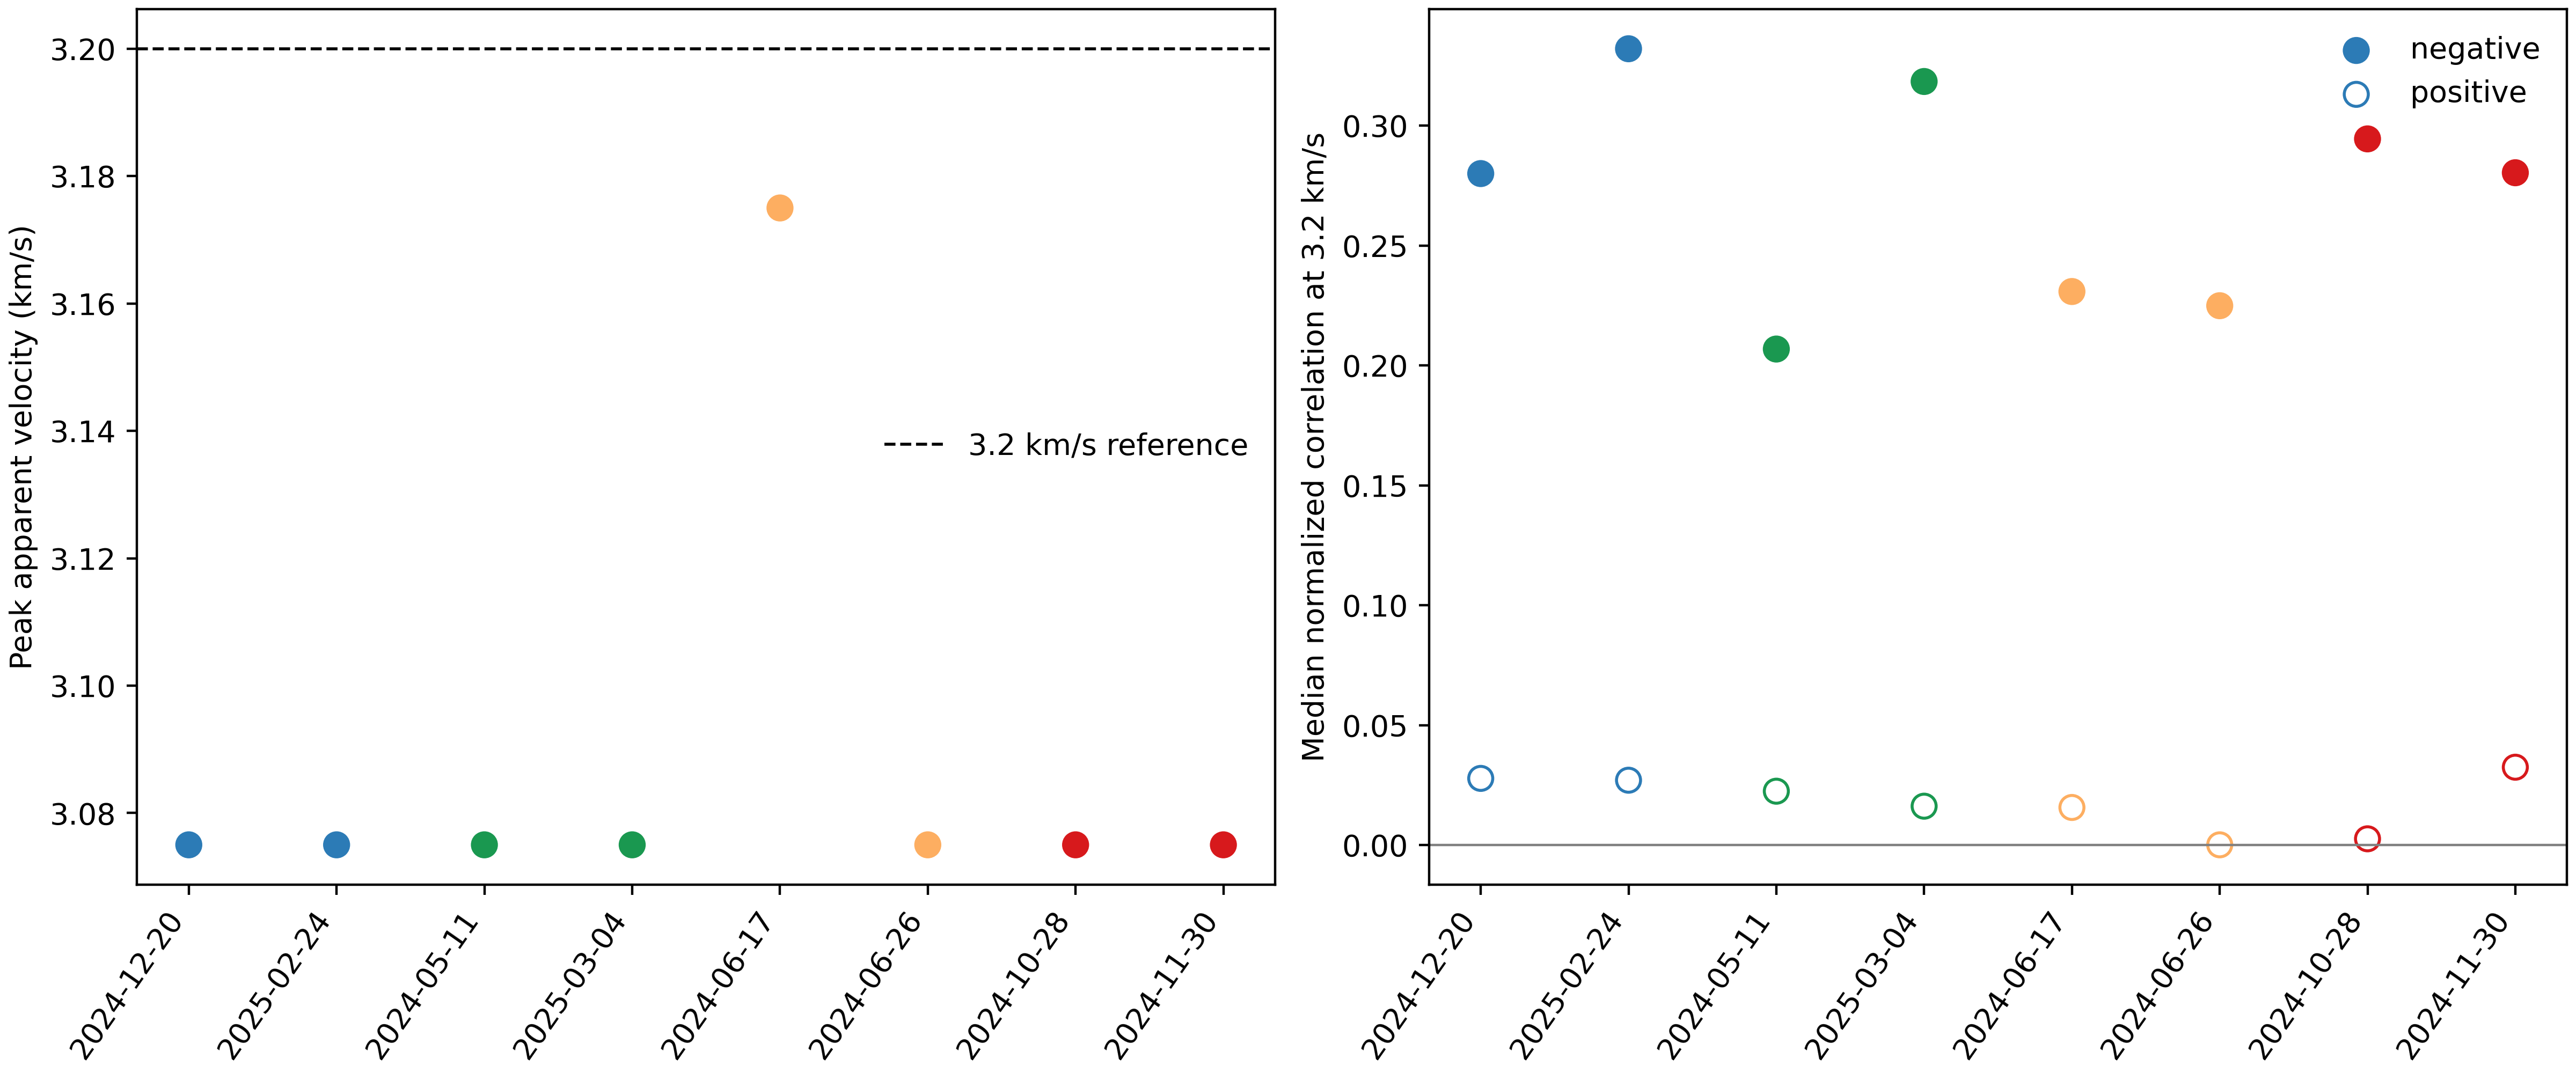
\includegraphics[width=0.98\linewidth]{ambient_transfer/fk_seasonal_day_comparison.png}
\caption{\textbf{Eight-day seasonal validation of the ambient signed F--K observable.} Each selected date was processed independently with the channel-0 top-source geometry, measured 1.020952-m spacing, 5--20-Hz preprocessing, and fixed signed velocity masks before aggregation. The negative branch reaches 3.075~km~s$^{-1}$ with score 0.279 and receiver-permutation $p=0.0002$ across 11,523 weighted files. The positive branch is not significant ($p=0.978$), the two-sided branch remains enhanced ($p=0.0026$), and the exact-resolution unfiltered control is weak ($p=0.343$). The figure demonstrates seasonal repeatability of a directionally selected transfer observable; because the negative wedge contains the target velocity interval by construction, it is not an independent formation-velocity estimate or an exact reproduction of the 2017 acquisition.}\end{figure}

\subsection{Completed frequency-band and anomaly diagnostics}
The frequency-band scan processed four ten-file blocks per selected day in 3--8, 5--12, 8--20, and 15--30~Hz bands. The 3--8-Hz control is the most stable, with median early and late apparent velocities of approximately 3.15 and 3.12~km~s$^{-1}$ and a median descriptive breakpoint near 425~m. Higher-frequency row-maximum fits are less stable and sometimes yield nonphysical late-branch values, so they are retained as sensitivity diagnostics rather than independent geological constraints. The full anomaly postprocess contains 1,167 products across nine dates and places the descriptive transition broadly near 350--425~m, not uniquely at 500--520~m.

\takeaway{The seasonal result is robust as a selected directional observable. The apparent spatial transition is repeatable but broad, frequency-dependent, and conditional on fiber-coordinate registration; it is not yet a lithologic boundary or $V_P$ inversion.}

\subsection{Anti-alias preprocessing sensitivity pilot}
\figquestion{Does the short-stack F--K result depend materially on direct factor-of-two decimation?}

The pilot compares the current direct slicing path, explicit anti-aliased polyphase resampling along both time and channel axes, and full-resolution processing. The same normalized correlations, 5--20-Hz bandpass, 2.5--4.5~km~s$^{-1}$ signed wedge, and receiver-permutation nulls are used in all paths. For the first 30 one-minute records on 2024-12-20, the direct path peaks at 1.875~km~s$^{-1}$ ($p=1.00$), the anti-aliased path at 1.850~km~s$^{-1}$ ($p=0.990$), and the full-resolution path at 1.925~km~s$^{-1}$ ($p=0.910$). These are all weak short-stack controls and differ by only 75~m~s$^{-1}$.

The pilot is reassuring about gross preprocessing sensitivity but does not validate the long-stack seasonal signal: 30 minutes is much shorter than the five-hour and complete-day products. A longer anti-aliased-versus-direct comparison remains the next robustness run.

\begin{figure}[H]
\centering
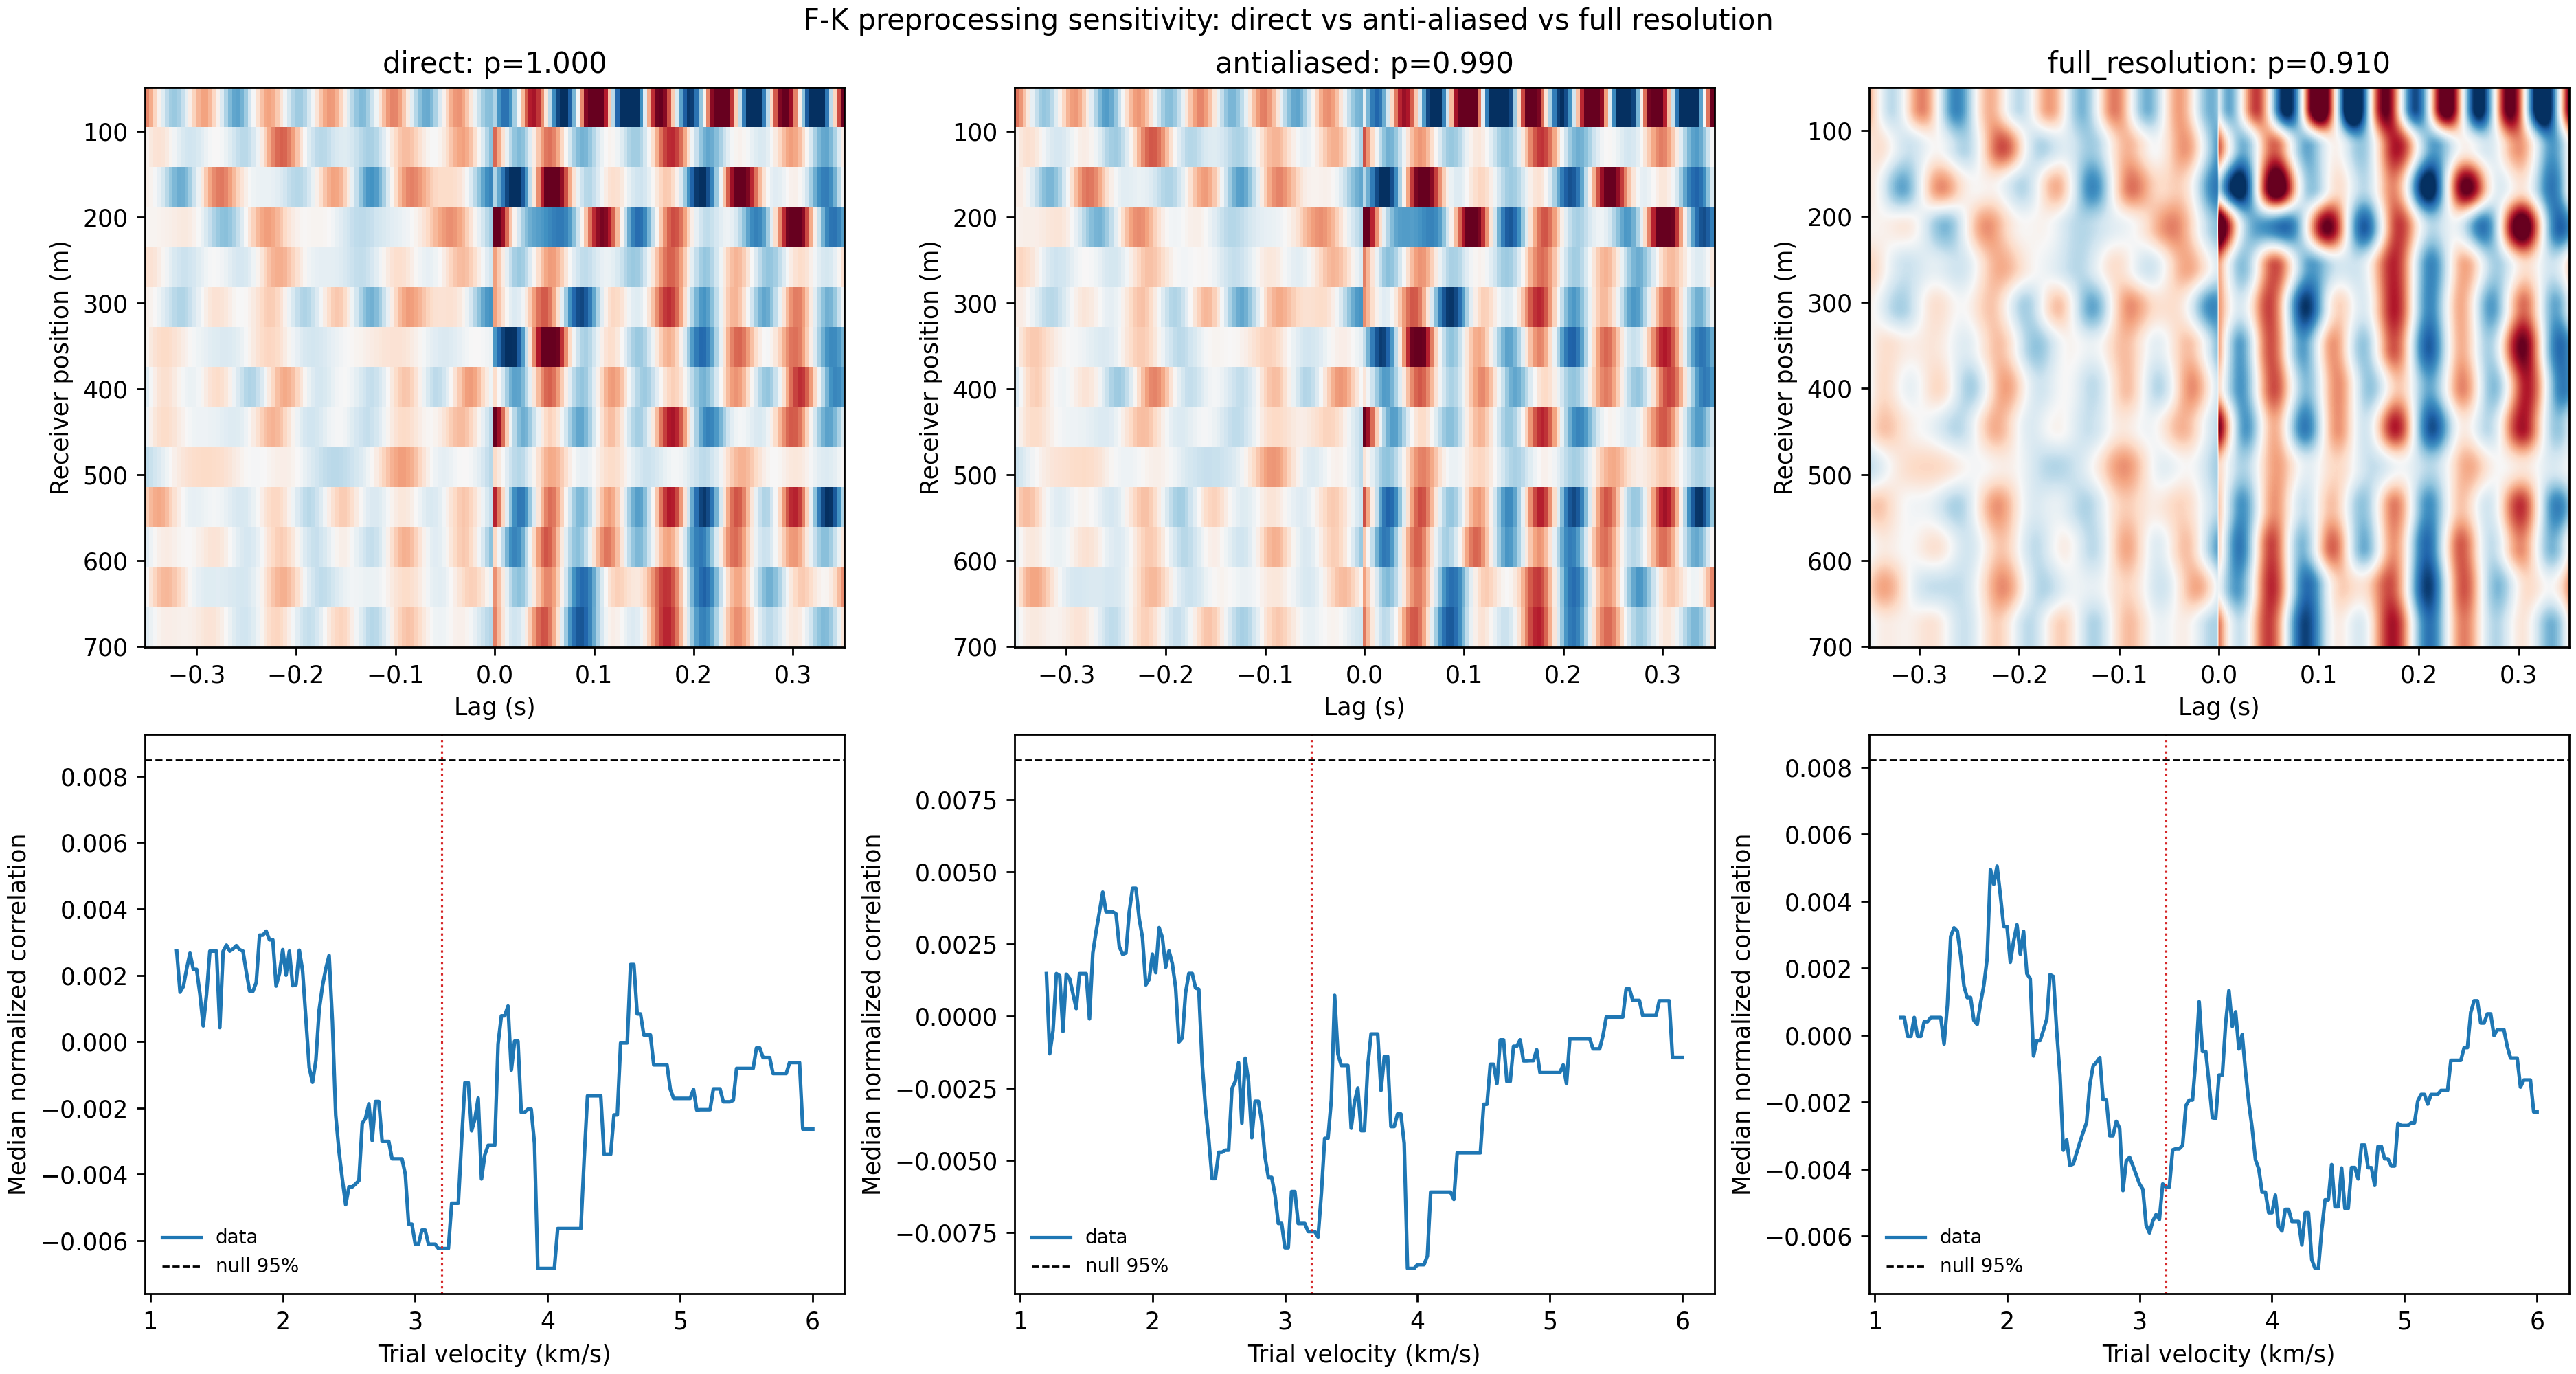
\includegraphics[width=0.98\linewidth]{ambient_transfer/alias_sensitivity_2024-12-20_start0_n30.png}
\caption{\textbf{Anti-alias preprocessing sensitivity for a 30-minute ambient pilot.} Columns compare direct factor-of-two slicing, explicit anti-aliased polyphase resampling along the time and channel axes, and full-resolution processing. The upper row shows top-source correlation sections; the lower row shows trial-velocity scores with receiver-permutation 95th-percentile thresholds. All three paths are weak and nonsignificant over this short interval, with peak velocities from 1.850 to 1.925~km~s$^{-1}$. The result is a preprocessing control rather than a test of the full seasonal F--K signal; the longer-stack comparison is required before declaring the seasonal result insensitive to decimation.}\end{figure}

\takeaway{v41 promotes the completed seasonal, unfiltered, frequency-band, and anti-alias products. The defensible claim is a repeatable, conditional negative signed F--K observable near 3.075~km~s$^{-1}$, with a broad processing-sensitive spatial transition and an anti-alias pilot that is reassuring but not yet long-stack validation.}

\end{document}
